\documentclass[twoside]{book}

% Packages required by doxygen
\usepackage{fixltx2e}
\usepackage{calc}
\usepackage{doxygen}
\usepackage[export]{adjustbox} % also loads graphicx
\usepackage{graphicx}
\usepackage[utf8]{inputenc}
\usepackage{makeidx}
\usepackage{multicol}
\usepackage{multirow}
\PassOptionsToPackage{warn}{textcomp}
\usepackage{textcomp}
\usepackage[nointegrals]{wasysym}
\usepackage[table]{xcolor}

% Font selection
\usepackage[T1]{fontenc}
\usepackage[scaled=.90]{helvet}
\usepackage{courier}
\usepackage{amssymb}
\usepackage{sectsty}
\renewcommand{\familydefault}{\sfdefault}
\allsectionsfont{%
  \fontseries{bc}\selectfont%
  \color{darkgray}%
}
\renewcommand{\DoxyLabelFont}{%
  \fontseries{bc}\selectfont%
  \color{darkgray}%
}
\newcommand{\+}{\discretionary{\mbox{\scriptsize$\hookleftarrow$}}{}{}}

% Page & text layout
\usepackage{geometry}
\geometry{%
  a4paper,%
  top=2.5cm,%
  bottom=2.5cm,%
  left=2.5cm,%
  right=2.5cm%
}
\tolerance=750
\hfuzz=15pt
\hbadness=750
\setlength{\emergencystretch}{15pt}
\setlength{\parindent}{0cm}
\setlength{\parskip}{3ex plus 2ex minus 2ex}
\makeatletter
\renewcommand{\paragraph}{%
  \@startsection{paragraph}{4}{0ex}{-1.0ex}{1.0ex}{%
    \normalfont\normalsize\bfseries\SS@parafont%
  }%
}
\renewcommand{\subparagraph}{%
  \@startsection{subparagraph}{5}{0ex}{-1.0ex}{1.0ex}{%
    \normalfont\normalsize\bfseries\SS@subparafont%
  }%
}
\makeatother

% Headers & footers
\usepackage{fancyhdr}
\pagestyle{fancyplain}
\fancyhead[LE]{\fancyplain{}{\bfseries\thepage}}
\fancyhead[CE]{\fancyplain{}{}}
\fancyhead[RE]{\fancyplain{}{\bfseries\leftmark}}
\fancyhead[LO]{\fancyplain{}{\bfseries\rightmark}}
\fancyhead[CO]{\fancyplain{}{}}
\fancyhead[RO]{\fancyplain{}{\bfseries\thepage}}
\fancyfoot[LE]{\fancyplain{}{}}
\fancyfoot[CE]{\fancyplain{}{}}
\fancyfoot[RE]{\fancyplain{}{\bfseries\scriptsize Generated by Doxygen }}
\fancyfoot[LO]{\fancyplain{}{\bfseries\scriptsize Generated by Doxygen }}
\fancyfoot[CO]{\fancyplain{}{}}
\fancyfoot[RO]{\fancyplain{}{}}
\renewcommand{\footrulewidth}{0.4pt}
\renewcommand{\chaptermark}[1]{%
  \markboth{#1}{}%
}
\renewcommand{\sectionmark}[1]{%
  \markright{\thesection\ #1}%
}

% Indices & bibliography
\usepackage{natbib}
\usepackage[titles]{tocloft}
\setcounter{tocdepth}{3}
\setcounter{secnumdepth}{5}
\makeindex

% Hyperlinks (required, but should be loaded last)
\usepackage{ifpdf}
\ifpdf
  \usepackage[pdftex,pagebackref=true]{hyperref}
\else
  \usepackage[ps2pdf,pagebackref=true]{hyperref}
\fi
\hypersetup{%
  colorlinks=true,%
  linkcolor=blue,%
  citecolor=blue,%
  unicode%
}

% Custom commands
\newcommand{\clearemptydoublepage}{%
  \newpage{\pagestyle{empty}\cleardoublepage}%
}

\usepackage{caption}
\captionsetup{labelsep=space,justification=centering,font={bf},singlelinecheck=off,skip=4pt,position=top}

%===== C O N T E N T S =====

\begin{document}

% Titlepage & ToC
\hypersetup{pageanchor=false,
             bookmarksnumbered=true,
             pdfencoding=unicode
            }
\pagenumbering{alph}
\begin{titlepage}
\vspace*{7cm}
\begin{center}%
{\Large My Project }\\
\vspace*{1cm}
{\large Generated by Doxygen 1.8.13}\\
\end{center}
\end{titlepage}
\clearemptydoublepage
\pagenumbering{roman}
\tableofcontents
\clearemptydoublepage
\pagenumbering{arabic}
\hypersetup{pageanchor=true}

%--- Begin generated contents ---
\chapter{Deprecated List}
\label{deprecated}
\Hypertarget{deprecated}

\begin{DoxyRefList}
\item[\label{deprecated__deprecated000001}%
\Hypertarget{deprecated__deprecated000001}%
Member \hyperlink{coindex-getopt_8h_a78a0cd581698415a62f68214603b1a30}{cmdline\+\_\+parser2} (int argc, char $\ast$$\ast$argv, struct \hyperlink{structgengetopt__args__info}{gengetopt\+\_\+args\+\_\+info} $\ast$args\+\_\+info, int override, int initialize, int check\+\_\+required)]use \hyperlink{coindex-getopt_8h_ac7bb5d76f3f56d1c0b3b531f11ac6f07}{cmdline\+\_\+parser\+\_\+ext()} instead 

use \hyperlink{coindex-getopt_8h_ac7bb5d76f3f56d1c0b3b531f11ac6f07}{cmdline\+\_\+parser\+\_\+ext()} instead 

use \hyperlink{coindex-getopt_8h_ac7bb5d76f3f56d1c0b3b531f11ac6f07}{cmdline\+\_\+parser\+\_\+ext()} instead 

use \hyperlink{coindex-getopt_8h_ac7bb5d76f3f56d1c0b3b531f11ac6f07}{cmdline\+\_\+parser\+\_\+ext()} instead 
\end{DoxyRefList}
\chapter{Hierarchical Index}
\section{Class Hierarchy}
This inheritance list is sorted roughly, but not completely, alphabetically\+:\begin{DoxyCompactList}
\item \contentsline{section}{A}{\pageref{classA}}{}
\item \contentsline{section}{Classic\+Cipher}{\pageref{classClassicCipher}}{}
\begin{DoxyCompactList}
\item \contentsline{section}{Vigenere\+Cipher}{\pageref{classVigenereCipher}}{}
\begin{DoxyCompactList}
\item \contentsline{section}{Vigenere\+Breaker}{\pageref{classVigenereBreaker}}{}
\end{DoxyCompactList}
\end{DoxyCompactList}
\item \contentsline{section}{cmdline\+\_\+parser\+\_\+params}{\pageref{structcmdline__parser__params}}{}
\item \contentsline{section}{custom\+\_\+getopt\+\_\+data}{\pageref{structcustom__getopt__data}}{}
\item \contentsline{section}{gengetopt\+\_\+args\+\_\+info}{\pageref{structgengetopt__args__info}}{}
\item \contentsline{section}{option}{\pageref{structoption}}{}
\item \contentsline{section}{P\+R\+NG}{\pageref{classPRNG}}{}
\begin{DoxyCompactList}
\item \contentsline{section}{Blum\+Blum\+Shub\+Generator}{\pageref{classBlumBlumShubGenerator}}{}
\end{DoxyCompactList}
\end{DoxyCompactList}

\chapter{Class Index}
\section{Class List}
Here are the classes, structs, unions and interfaces with brief descriptions\+:\begin{DoxyCompactList}
\item\contentsline{section}{\hyperlink{classBlumBlumShubGenerator}{Blum\+Blum\+Shub\+Generator} }{\pageref{classBlumBlumShubGenerator}}{}
\item\contentsline{section}{\hyperlink{classPRNG}{P\+R\+NG} }{\pageref{classPRNG}}{}
\end{DoxyCompactList}

\chapter{File Index}
\section{File List}
Here is a list of all documented files with brief descriptions\+:\begin{DoxyCompactList}
\item\contentsline{section}{/home/sinflair/\+P/crypto/\+A\+K/src/\+Praktikum-\/\+D\+E\+S/{\bfseries Block\+Cipher.\+h} }{\pageref{BlockCipher_8h}}{}
\item\contentsline{section}{/home/sinflair/\+P/crypto/\+A\+K/src/\+Praktikum-\/\+D\+E\+S/{\bfseries byte.\+h} }{\pageref{byte_8h}}{}
\item\contentsline{section}{/home/sinflair/\+P/crypto/\+A\+K/src/\+Praktikum-\/\+D\+E\+S/{\bfseries catch.\+hpp} }{\pageref{catch_8hpp}}{}
\item\contentsline{section}{/home/sinflair/\+P/crypto/\+A\+K/src/\+Praktikum-\/\+D\+E\+S/\hyperlink{des-getopt_8h}{des-\/getopt.\+h} \\*The header file for the command line option parser generated by G\+NU Gengetopt version 2.\+22.\+6 \href{http://www.gnu.org/software/gengetopt}{\tt http\+://www.\+gnu.\+org/software/gengetopt}. DO N\+OT modify this file, since it can be overwritten }{\pageref{des-getopt_8h}}{}
\item\contentsline{section}{/home/sinflair/\+P/crypto/\+A\+K/src/\+Praktikum-\/\+D\+E\+S/{\bfseries D\+E\+S\+Cipher.\+h} }{\pageref{DESCipher_8h}}{}
\end{DoxyCompactList}

\chapter{Class Documentation}
\hypertarget{structCatch_1_1always__false}{}\section{Catch\+:\+:always\+\_\+false$<$ T $>$ Struct Template Reference}
\label{structCatch_1_1always__false}\index{Catch\+::always\+\_\+false$<$ T $>$@{Catch\+::always\+\_\+false$<$ T $>$}}


Inheritance diagram for Catch\+:\+:always\+\_\+false$<$ T $>$\+:
\nopagebreak
\begin{figure}[H]
\begin{center}
\leavevmode
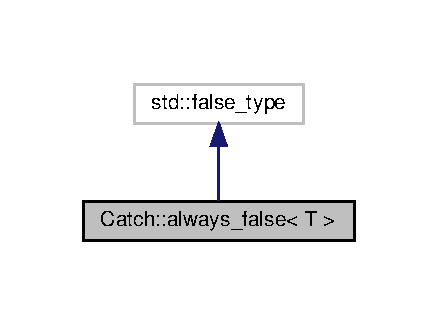
\includegraphics[width=210pt]{structCatch_1_1always__false__inherit__graph}
\end{center}
\end{figure}


Collaboration diagram for Catch\+:\+:always\+\_\+false$<$ T $>$\+:
\nopagebreak
\begin{figure}[H]
\begin{center}
\leavevmode
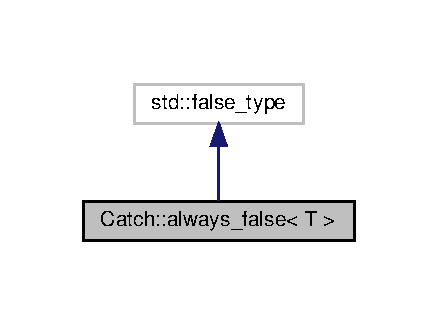
\includegraphics[width=210pt]{structCatch_1_1always__false__coll__graph}
\end{center}
\end{figure}


The documentation for this struct was generated from the following file\+:\begin{DoxyCompactItemize}
\item 
/home/sinflair/\+P/crypto/\+A\+K/src/\+Praktikum-\/\+D\+E\+S/catch.\+hpp\end{DoxyCompactItemize}

\hypertarget{classCatch_1_1Detail_1_1Approx}{}\section{Catch\+:\+:Detail\+:\+:Approx Class Reference}
\label{classCatch_1_1Detail_1_1Approx}\index{Catch\+::\+Detail\+::\+Approx@{Catch\+::\+Detail\+::\+Approx}}
\subsection*{Public Member Functions}
\begin{DoxyCompactItemize}
\item 
\mbox{\Hypertarget{classCatch_1_1Detail_1_1Approx_a1a8618ea8db08c66bd3d9fe8f74b957a}\label{classCatch_1_1Detail_1_1Approx_a1a8618ea8db08c66bd3d9fe8f74b957a}} 
{\bfseries Approx} (double value)
\item 
\mbox{\Hypertarget{classCatch_1_1Detail_1_1Approx_aa9adf5f05e641df770039543d5067d30}\label{classCatch_1_1Detail_1_1Approx_aa9adf5f05e641df770039543d5067d30}} 
\hyperlink{classCatch_1_1Detail_1_1Approx}{Approx} {\bfseries operator-\/} () const
\item 
\mbox{\Hypertarget{classCatch_1_1Detail_1_1Approx_ad8b2757f4804f9a1d3fa674efb98c20e}\label{classCatch_1_1Detail_1_1Approx_ad8b2757f4804f9a1d3fa674efb98c20e}} 
{\footnotesize template$<$typename T , typename  = typename std\+::enable\+\_\+if$<$std\+::is\+\_\+constructible$<$double, T$>$\+::value$>$\+::type$>$ }\\\hyperlink{classCatch_1_1Detail_1_1Approx}{Approx} {\bfseries operator()} (T const \&value)
\item 
\mbox{\Hypertarget{classCatch_1_1Detail_1_1Approx_ab14b979fa8a37f21d037157fabed4072}\label{classCatch_1_1Detail_1_1Approx_ab14b979fa8a37f21d037157fabed4072}} 
{\footnotesize template$<$typename T , typename  = typename std\+::enable\+\_\+if$<$std\+::is\+\_\+constructible$<$double, T$>$\+::value$>$\+::type$>$ }\\{\bfseries Approx} (T const \&value)
\item 
\mbox{\Hypertarget{classCatch_1_1Detail_1_1Approx_acd26adba86a066b9f40dad467f23bc85}\label{classCatch_1_1Detail_1_1Approx_acd26adba86a066b9f40dad467f23bc85}} 
{\footnotesize template$<$typename T , typename  = typename std\+::enable\+\_\+if$<$std\+::is\+\_\+constructible$<$double, T$>$\+::value$>$\+::type$>$ }\\\hyperlink{classCatch_1_1Detail_1_1Approx}{Approx} \& {\bfseries epsilon} (T const \&new\+Epsilon)
\item 
\mbox{\Hypertarget{classCatch_1_1Detail_1_1Approx_a6467dc18791e1a1f4c15c4fb63cf5051}\label{classCatch_1_1Detail_1_1Approx_a6467dc18791e1a1f4c15c4fb63cf5051}} 
{\footnotesize template$<$typename T , typename  = typename std\+::enable\+\_\+if$<$std\+::is\+\_\+constructible$<$double, T$>$\+::value$>$\+::type$>$ }\\\hyperlink{classCatch_1_1Detail_1_1Approx}{Approx} \& {\bfseries margin} (T const \&new\+Margin)
\item 
\mbox{\Hypertarget{classCatch_1_1Detail_1_1Approx_a8f4d2def2920a3840d3271f6d9c5ede2}\label{classCatch_1_1Detail_1_1Approx_a8f4d2def2920a3840d3271f6d9c5ede2}} 
{\footnotesize template$<$typename T , typename  = typename std\+::enable\+\_\+if$<$std\+::is\+\_\+constructible$<$double, T$>$\+::value$>$\+::type$>$ }\\\hyperlink{classCatch_1_1Detail_1_1Approx}{Approx} \& {\bfseries scale} (T const \&new\+Scale)
\item 
\mbox{\Hypertarget{classCatch_1_1Detail_1_1Approx_a972fd9ac60607483263f1b0f0f9955e6}\label{classCatch_1_1Detail_1_1Approx_a972fd9ac60607483263f1b0f0f9955e6}} 
std\+::string {\bfseries to\+String} () const
\end{DoxyCompactItemize}
\subsection*{Static Public Member Functions}
\begin{DoxyCompactItemize}
\item 
\mbox{\Hypertarget{classCatch_1_1Detail_1_1Approx_aaf86dc0ee92272ac2d9839197a07951d}\label{classCatch_1_1Detail_1_1Approx_aaf86dc0ee92272ac2d9839197a07951d}} 
static \hyperlink{classCatch_1_1Detail_1_1Approx}{Approx} {\bfseries custom} ()
\end{DoxyCompactItemize}
\subsection*{Private Member Functions}
\begin{DoxyCompactItemize}
\item 
\mbox{\Hypertarget{classCatch_1_1Detail_1_1Approx_af53c48227a7b654da58adeb1d360b715}\label{classCatch_1_1Detail_1_1Approx_af53c48227a7b654da58adeb1d360b715}} 
bool {\bfseries equality\+Comparison\+Impl} (double other) const
\item 
\mbox{\Hypertarget{classCatch_1_1Detail_1_1Approx_aff04b8b32edc707138eb395ed45ec576}\label{classCatch_1_1Detail_1_1Approx_aff04b8b32edc707138eb395ed45ec576}} 
void {\bfseries set\+Margin} (double margin)
\item 
\mbox{\Hypertarget{classCatch_1_1Detail_1_1Approx_a28fd65e069b698bc7ae8f060bfbcd6b6}\label{classCatch_1_1Detail_1_1Approx_a28fd65e069b698bc7ae8f060bfbcd6b6}} 
void {\bfseries set\+Epsilon} (double epsilon)
\end{DoxyCompactItemize}
\subsection*{Private Attributes}
\begin{DoxyCompactItemize}
\item 
\mbox{\Hypertarget{classCatch_1_1Detail_1_1Approx_af17c8e869ae7a55d14b99eb18e178114}\label{classCatch_1_1Detail_1_1Approx_af17c8e869ae7a55d14b99eb18e178114}} 
double {\bfseries m\+\_\+epsilon}
\item 
\mbox{\Hypertarget{classCatch_1_1Detail_1_1Approx_a4262a7e821eec507b424c335121ea0d8}\label{classCatch_1_1Detail_1_1Approx_a4262a7e821eec507b424c335121ea0d8}} 
double {\bfseries m\+\_\+margin}
\item 
\mbox{\Hypertarget{classCatch_1_1Detail_1_1Approx_a65e9bdab9113ff3300b45f0a4e048dd7}\label{classCatch_1_1Detail_1_1Approx_a65e9bdab9113ff3300b45f0a4e048dd7}} 
double {\bfseries m\+\_\+scale}
\item 
\mbox{\Hypertarget{classCatch_1_1Detail_1_1Approx_af7aeef703bd591f5ec85407b1dac053c}\label{classCatch_1_1Detail_1_1Approx_af7aeef703bd591f5ec85407b1dac053c}} 
double {\bfseries m\+\_\+value}
\end{DoxyCompactItemize}
\subsection*{Friends}
\begin{DoxyCompactItemize}
\item 
\mbox{\Hypertarget{classCatch_1_1Detail_1_1Approx_ab38782a37d09b527ca5e126dbf433dda}\label{classCatch_1_1Detail_1_1Approx_ab38782a37d09b527ca5e126dbf433dda}} 
{\footnotesize template$<$typename T , typename  = typename std\+::enable\+\_\+if$<$std\+::is\+\_\+constructible$<$double, T$>$\+::value$>$\+::type$>$ }\\bool {\bfseries operator==} (const T \&lhs, \hyperlink{classCatch_1_1Detail_1_1Approx}{Approx} const \&rhs)
\item 
\mbox{\Hypertarget{classCatch_1_1Detail_1_1Approx_a0e5ef1957d4c38d7857005909c613743}\label{classCatch_1_1Detail_1_1Approx_a0e5ef1957d4c38d7857005909c613743}} 
{\footnotesize template$<$typename T , typename  = typename std\+::enable\+\_\+if$<$std\+::is\+\_\+constructible$<$double, T$>$\+::value$>$\+::type$>$ }\\bool {\bfseries operator==} (\hyperlink{classCatch_1_1Detail_1_1Approx}{Approx} const \&lhs, const T \&rhs)
\item 
\mbox{\Hypertarget{classCatch_1_1Detail_1_1Approx_a29696f14ebd51887c8c88e771d12ef54}\label{classCatch_1_1Detail_1_1Approx_a29696f14ebd51887c8c88e771d12ef54}} 
{\footnotesize template$<$typename T , typename  = typename std\+::enable\+\_\+if$<$std\+::is\+\_\+constructible$<$double, T$>$\+::value$>$\+::type$>$ }\\bool {\bfseries operator!=} (T const \&lhs, \hyperlink{classCatch_1_1Detail_1_1Approx}{Approx} const \&rhs)
\item 
\mbox{\Hypertarget{classCatch_1_1Detail_1_1Approx_a31d62e3c35abb86cf25e02601966ca5d}\label{classCatch_1_1Detail_1_1Approx_a31d62e3c35abb86cf25e02601966ca5d}} 
{\footnotesize template$<$typename T , typename  = typename std\+::enable\+\_\+if$<$std\+::is\+\_\+constructible$<$double, T$>$\+::value$>$\+::type$>$ }\\bool {\bfseries operator!=} (\hyperlink{classCatch_1_1Detail_1_1Approx}{Approx} const \&lhs, T const \&rhs)
\item 
\mbox{\Hypertarget{classCatch_1_1Detail_1_1Approx_a0369de03e81bc2ceaf6c9d830476bd49}\label{classCatch_1_1Detail_1_1Approx_a0369de03e81bc2ceaf6c9d830476bd49}} 
{\footnotesize template$<$typename T , typename  = typename std\+::enable\+\_\+if$<$std\+::is\+\_\+constructible$<$double, T$>$\+::value$>$\+::type$>$ }\\bool {\bfseries operator$<$=} (T const \&lhs, \hyperlink{classCatch_1_1Detail_1_1Approx}{Approx} const \&rhs)
\item 
\mbox{\Hypertarget{classCatch_1_1Detail_1_1Approx_a6040b908588745570847d7ae8483b091}\label{classCatch_1_1Detail_1_1Approx_a6040b908588745570847d7ae8483b091}} 
{\footnotesize template$<$typename T , typename  = typename std\+::enable\+\_\+if$<$std\+::is\+\_\+constructible$<$double, T$>$\+::value$>$\+::type$>$ }\\bool {\bfseries operator$<$=} (\hyperlink{classCatch_1_1Detail_1_1Approx}{Approx} const \&lhs, T const \&rhs)
\item 
\mbox{\Hypertarget{classCatch_1_1Detail_1_1Approx_affd27efc62be386daeecb7a09e828d44}\label{classCatch_1_1Detail_1_1Approx_affd27efc62be386daeecb7a09e828d44}} 
{\footnotesize template$<$typename T , typename  = typename std\+::enable\+\_\+if$<$std\+::is\+\_\+constructible$<$double, T$>$\+::value$>$\+::type$>$ }\\bool {\bfseries operator$>$=} (T const \&lhs, \hyperlink{classCatch_1_1Detail_1_1Approx}{Approx} const \&rhs)
\item 
\mbox{\Hypertarget{classCatch_1_1Detail_1_1Approx_a5899b8a36725406701e2ebded2971ee6}\label{classCatch_1_1Detail_1_1Approx_a5899b8a36725406701e2ebded2971ee6}} 
{\footnotesize template$<$typename T , typename  = typename std\+::enable\+\_\+if$<$std\+::is\+\_\+constructible$<$double, T$>$\+::value$>$\+::type$>$ }\\bool {\bfseries operator$>$=} (\hyperlink{classCatch_1_1Detail_1_1Approx}{Approx} const \&lhs, T const \&rhs)
\end{DoxyCompactItemize}


The documentation for this class was generated from the following file\+:\begin{DoxyCompactItemize}
\item 
/home/sinflair/\+P/crypto/\+A\+K/src/\+Praktikum-\/\+D\+E\+S/catch.\+hpp\end{DoxyCompactItemize}

\hypertarget{structCatch_1_1Matchers_1_1Vector_1_1ApproxMatcher}{}\section{Catch\+:\+:Matchers\+:\+:Vector\+:\+:Approx\+Matcher$<$ T $>$ Struct Template Reference}
\label{structCatch_1_1Matchers_1_1Vector_1_1ApproxMatcher}\index{Catch\+::\+Matchers\+::\+Vector\+::\+Approx\+Matcher$<$ T $>$@{Catch\+::\+Matchers\+::\+Vector\+::\+Approx\+Matcher$<$ T $>$}}


Inheritance diagram for Catch\+:\+:Matchers\+:\+:Vector\+:\+:Approx\+Matcher$<$ T $>$\+:
\nopagebreak
\begin{figure}[H]
\begin{center}
\leavevmode
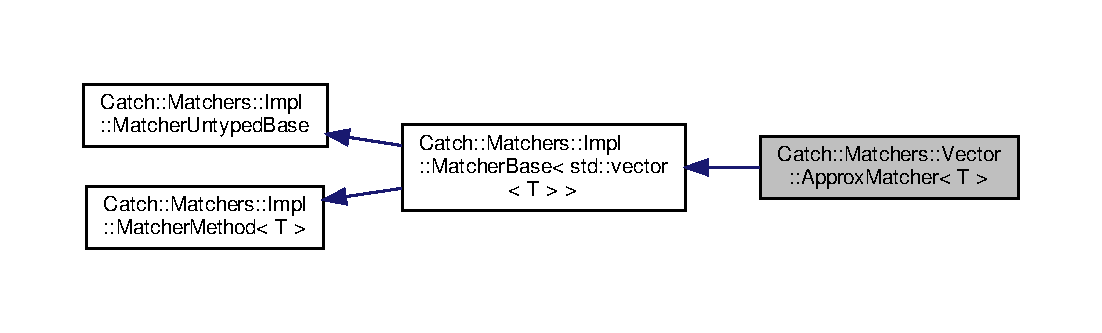
\includegraphics[width=350pt]{structCatch_1_1Matchers_1_1Vector_1_1ApproxMatcher__inherit__graph}
\end{center}
\end{figure}


Collaboration diagram for Catch\+:\+:Matchers\+:\+:Vector\+:\+:Approx\+Matcher$<$ T $>$\+:
\nopagebreak
\begin{figure}[H]
\begin{center}
\leavevmode
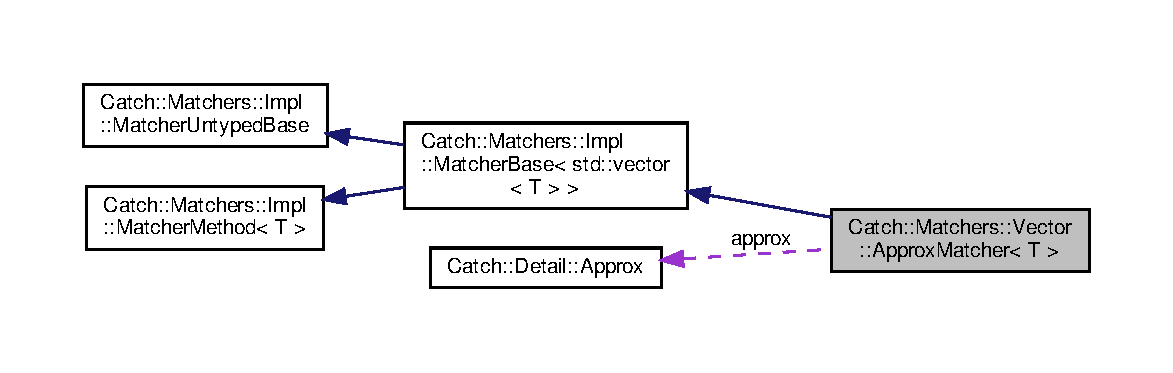
\includegraphics[width=350pt]{structCatch_1_1Matchers_1_1Vector_1_1ApproxMatcher__coll__graph}
\end{center}
\end{figure}
\subsection*{Public Member Functions}
\begin{DoxyCompactItemize}
\item 
\mbox{\Hypertarget{structCatch_1_1Matchers_1_1Vector_1_1ApproxMatcher_a55e8f7018104e0730eef656a61646870}\label{structCatch_1_1Matchers_1_1Vector_1_1ApproxMatcher_a55e8f7018104e0730eef656a61646870}} 
{\bfseries Approx\+Matcher} (std\+::vector$<$ T $>$ const \&comparator)
\item 
\mbox{\Hypertarget{structCatch_1_1Matchers_1_1Vector_1_1ApproxMatcher_a9cbd62093c4c123f1984726e1a14b270}\label{structCatch_1_1Matchers_1_1Vector_1_1ApproxMatcher_a9cbd62093c4c123f1984726e1a14b270}} 
bool {\bfseries match} (std\+::vector$<$ T $>$ const \&v) const override
\item 
\mbox{\Hypertarget{structCatch_1_1Matchers_1_1Vector_1_1ApproxMatcher_a1a9237e24c513c1448fa0624b3e14232}\label{structCatch_1_1Matchers_1_1Vector_1_1ApproxMatcher_a1a9237e24c513c1448fa0624b3e14232}} 
std\+::string {\bfseries describe} () const override
\item 
\mbox{\Hypertarget{structCatch_1_1Matchers_1_1Vector_1_1ApproxMatcher_a319b3a7fa9d0f401bfda5b45dafbbf5a}\label{structCatch_1_1Matchers_1_1Vector_1_1ApproxMatcher_a319b3a7fa9d0f401bfda5b45dafbbf5a}} 
{\footnotesize template$<$typename  = typename std\+::enable\+\_\+if$<$std\+::is\+\_\+constructible$<$double, T$>$\+::value$>$\+::type$>$ }\\\hyperlink{structCatch_1_1Matchers_1_1Vector_1_1ApproxMatcher}{Approx\+Matcher} \& {\bfseries epsilon} (T const \&new\+Epsilon)
\item 
\mbox{\Hypertarget{structCatch_1_1Matchers_1_1Vector_1_1ApproxMatcher_ac3b3afb3e5a9ad9ee0516e0202e08959}\label{structCatch_1_1Matchers_1_1Vector_1_1ApproxMatcher_ac3b3afb3e5a9ad9ee0516e0202e08959}} 
{\footnotesize template$<$typename  = typename std\+::enable\+\_\+if$<$std\+::is\+\_\+constructible$<$double, T$>$\+::value$>$\+::type$>$ }\\\hyperlink{structCatch_1_1Matchers_1_1Vector_1_1ApproxMatcher}{Approx\+Matcher} \& {\bfseries margin} (T const \&new\+Margin)
\item 
\mbox{\Hypertarget{structCatch_1_1Matchers_1_1Vector_1_1ApproxMatcher_a8658dc0564e0f80f101e4574830a3b18}\label{structCatch_1_1Matchers_1_1Vector_1_1ApproxMatcher_a8658dc0564e0f80f101e4574830a3b18}} 
{\footnotesize template$<$typename  = typename std\+::enable\+\_\+if$<$std\+::is\+\_\+constructible$<$double, T$>$\+::value$>$\+::type$>$ }\\\hyperlink{structCatch_1_1Matchers_1_1Vector_1_1ApproxMatcher}{Approx\+Matcher} \& {\bfseries scale} (T const \&new\+Scale)
\end{DoxyCompactItemize}
\subsection*{Public Attributes}
\begin{DoxyCompactItemize}
\item 
\mbox{\Hypertarget{structCatch_1_1Matchers_1_1Vector_1_1ApproxMatcher_a1394b5913d30bdd1147e1941fc41af56}\label{structCatch_1_1Matchers_1_1Vector_1_1ApproxMatcher_a1394b5913d30bdd1147e1941fc41af56}} 
std\+::vector$<$ T $>$ const  \& {\bfseries m\+\_\+comparator}
\item 
\mbox{\Hypertarget{structCatch_1_1Matchers_1_1Vector_1_1ApproxMatcher_a5515447af58adb5dc48a5d300b9ae162}\label{structCatch_1_1Matchers_1_1Vector_1_1ApproxMatcher_a5515447af58adb5dc48a5d300b9ae162}} 
\hyperlink{classCatch_1_1Detail_1_1Approx}{Catch\+::\+Detail\+::\+Approx} {\bfseries approx} = Catch\+::\+Detail\+::\+Approx\+::custom()
\end{DoxyCompactItemize}
\subsection*{Additional Inherited Members}


The documentation for this struct was generated from the following file\+:\begin{DoxyCompactItemize}
\item 
/home/sinflair/\+P/crypto/\+A\+K/src/\+Praktikum-\/\+D\+E\+S/catch.\+hpp\end{DoxyCompactItemize}

\hypertarget{structCatch_1_1Generators_1_1as}{}\section{Catch\+:\+:Generators\+:\+:as$<$ T $>$ Struct Template Reference}
\label{structCatch_1_1Generators_1_1as}\index{Catch\+::\+Generators\+::as$<$ T $>$@{Catch\+::\+Generators\+::as$<$ T $>$}}


The documentation for this struct was generated from the following file\+:\begin{DoxyCompactItemize}
\item 
/home/sinflair/\+P/crypto/\+A\+K/src/\+Praktikum-\/\+D\+E\+S/catch.\+hpp\end{DoxyCompactItemize}

\hypertarget{classCatch_1_1AssertionHandler}{}\section{Catch\+:\+:Assertion\+Handler Class Reference}
\label{classCatch_1_1AssertionHandler}\index{Catch\+::\+Assertion\+Handler@{Catch\+::\+Assertion\+Handler}}


Collaboration diagram for Catch\+:\+:Assertion\+Handler\+:
\nopagebreak
\begin{figure}[H]
\begin{center}
\leavevmode
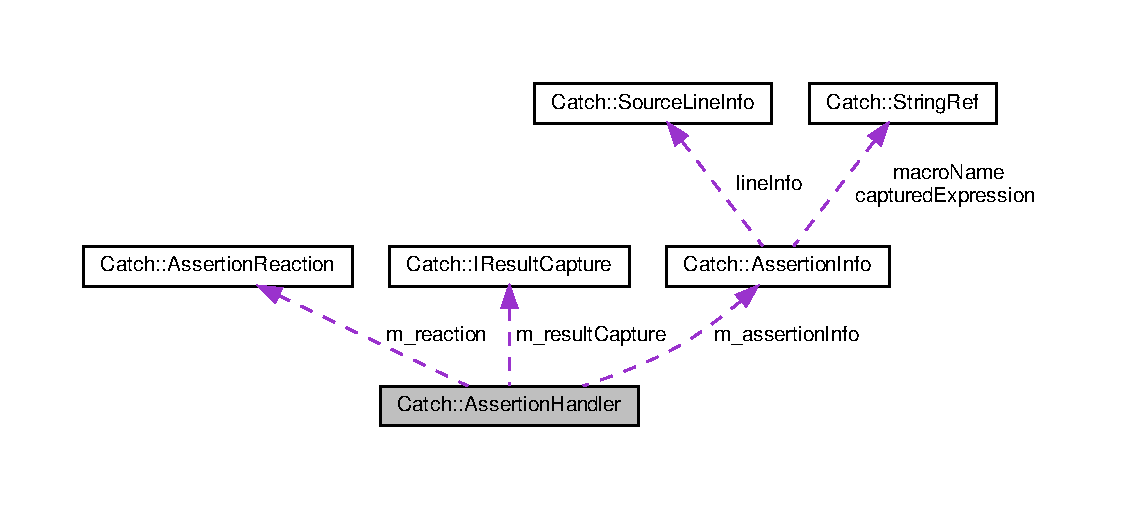
\includegraphics[width=350pt]{classCatch_1_1AssertionHandler__coll__graph}
\end{center}
\end{figure}
\subsection*{Public Member Functions}
\begin{DoxyCompactItemize}
\item 
\mbox{\Hypertarget{classCatch_1_1AssertionHandler_a32efbb1b56b71d758d4c2094bac1f1a9}\label{classCatch_1_1AssertionHandler_a32efbb1b56b71d758d4c2094bac1f1a9}} 
{\bfseries Assertion\+Handler} (\hyperlink{classCatch_1_1StringRef}{String\+Ref} const \&macro\+Name, \hyperlink{structCatch_1_1SourceLineInfo}{Source\+Line\+Info} const \&line\+Info, \hyperlink{classCatch_1_1StringRef}{String\+Ref} captured\+Expression, Result\+Disposition\+::\+Flags result\+Disposition)
\item 
\mbox{\Hypertarget{classCatch_1_1AssertionHandler_a2ef387e567bad90ec6e4b5bf5c367388}\label{classCatch_1_1AssertionHandler_a2ef387e567bad90ec6e4b5bf5c367388}} 
{\footnotesize template$<$typename T $>$ }\\void {\bfseries handle\+Expr} (\hyperlink{classCatch_1_1ExprLhs}{Expr\+Lhs}$<$ T $>$ const \&expr)
\item 
\mbox{\Hypertarget{classCatch_1_1AssertionHandler_afe14d9cf1b1c7f70dae439fbdb51d0c4}\label{classCatch_1_1AssertionHandler_afe14d9cf1b1c7f70dae439fbdb51d0c4}} 
void {\bfseries handle\+Expr} (\hyperlink{structCatch_1_1ITransientExpression}{I\+Transient\+Expression} const \&expr)
\item 
\mbox{\Hypertarget{classCatch_1_1AssertionHandler_abdb4c180ed83ec2858b2fb87712c516d}\label{classCatch_1_1AssertionHandler_abdb4c180ed83ec2858b2fb87712c516d}} 
void {\bfseries handle\+Message} (Result\+Was\+::\+Of\+Type result\+Type, \hyperlink{classCatch_1_1StringRef}{String\+Ref} const \&message)
\item 
\mbox{\Hypertarget{classCatch_1_1AssertionHandler_ab6caf765764a4064e90fce829eec201d}\label{classCatch_1_1AssertionHandler_ab6caf765764a4064e90fce829eec201d}} 
void {\bfseries handle\+Exception\+Thrown\+As\+Expected} ()
\item 
\mbox{\Hypertarget{classCatch_1_1AssertionHandler_a7764d0adb6ed5eeb10964f6abc02fab1}\label{classCatch_1_1AssertionHandler_a7764d0adb6ed5eeb10964f6abc02fab1}} 
void {\bfseries handle\+Unexpected\+Exception\+Not\+Thrown} ()
\item 
\mbox{\Hypertarget{classCatch_1_1AssertionHandler_a51e4936e3af43b74690cedae6d2e297a}\label{classCatch_1_1AssertionHandler_a51e4936e3af43b74690cedae6d2e297a}} 
void {\bfseries handle\+Exception\+Not\+Thrown\+As\+Expected} ()
\item 
\mbox{\Hypertarget{classCatch_1_1AssertionHandler_a67a194d5518f307c4a16faa03a7f7442}\label{classCatch_1_1AssertionHandler_a67a194d5518f307c4a16faa03a7f7442}} 
void {\bfseries handle\+Throwing\+Call\+Skipped} ()
\item 
\mbox{\Hypertarget{classCatch_1_1AssertionHandler_aa2504dad6a91f3645e5f52c932c11270}\label{classCatch_1_1AssertionHandler_aa2504dad6a91f3645e5f52c932c11270}} 
void {\bfseries handle\+Unexpected\+Inflight\+Exception} ()
\item 
\mbox{\Hypertarget{classCatch_1_1AssertionHandler_a878a9eb828d8a1863c8dcb6575f6f40e}\label{classCatch_1_1AssertionHandler_a878a9eb828d8a1863c8dcb6575f6f40e}} 
void {\bfseries complete} ()
\item 
\mbox{\Hypertarget{classCatch_1_1AssertionHandler_a6756bd5395c0ddd28764a9fb4612d5e4}\label{classCatch_1_1AssertionHandler_a6756bd5395c0ddd28764a9fb4612d5e4}} 
void {\bfseries set\+Completed} ()
\item 
\mbox{\Hypertarget{classCatch_1_1AssertionHandler_a193bb3999494c46457f3059184c6b251}\label{classCatch_1_1AssertionHandler_a193bb3999494c46457f3059184c6b251}} 
auto {\bfseries allow\+Throws} () const -\/$>$ bool
\end{DoxyCompactItemize}
\subsection*{Private Attributes}
\begin{DoxyCompactItemize}
\item 
\mbox{\Hypertarget{classCatch_1_1AssertionHandler_ad171e8724bb771d97949b7270f400303}\label{classCatch_1_1AssertionHandler_ad171e8724bb771d97949b7270f400303}} 
\hyperlink{structCatch_1_1AssertionInfo}{Assertion\+Info} {\bfseries m\+\_\+assertion\+Info}
\item 
\mbox{\Hypertarget{classCatch_1_1AssertionHandler_a8203c08a43a3761b5f400ee6587fad55}\label{classCatch_1_1AssertionHandler_a8203c08a43a3761b5f400ee6587fad55}} 
\hyperlink{structCatch_1_1AssertionReaction}{Assertion\+Reaction} {\bfseries m\+\_\+reaction}
\item 
\mbox{\Hypertarget{classCatch_1_1AssertionHandler_a5a756818dff781c155e8eb970d1d4c68}\label{classCatch_1_1AssertionHandler_a5a756818dff781c155e8eb970d1d4c68}} 
bool {\bfseries m\+\_\+completed} = false
\item 
\mbox{\Hypertarget{classCatch_1_1AssertionHandler_aea5283ee36124ce5c51dc2a697b22a39}\label{classCatch_1_1AssertionHandler_aea5283ee36124ce5c51dc2a697b22a39}} 
\hyperlink{structCatch_1_1IResultCapture}{I\+Result\+Capture} \& {\bfseries m\+\_\+result\+Capture}
\end{DoxyCompactItemize}


The documentation for this class was generated from the following file\+:\begin{DoxyCompactItemize}
\item 
/home/sinflair/\+P/crypto/\+A\+K/src/\+Praktikum-\/\+D\+E\+S/catch.\+hpp\end{DoxyCompactItemize}

\hypertarget{structCatch_1_1AssertionInfo}{}\section{Catch\+:\+:Assertion\+Info Struct Reference}
\label{structCatch_1_1AssertionInfo}\index{Catch\+::\+Assertion\+Info@{Catch\+::\+Assertion\+Info}}


Collaboration diagram for Catch\+:\+:Assertion\+Info\+:
\nopagebreak
\begin{figure}[H]
\begin{center}
\leavevmode
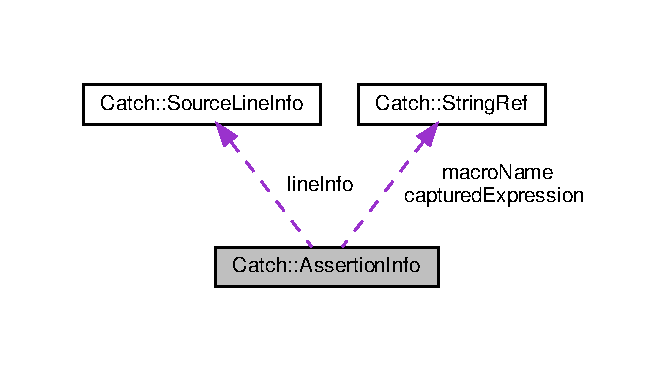
\includegraphics[width=321pt]{structCatch_1_1AssertionInfo__coll__graph}
\end{center}
\end{figure}
\subsection*{Public Attributes}
\begin{DoxyCompactItemize}
\item 
\mbox{\Hypertarget{structCatch_1_1AssertionInfo_aaf3fbb9f1fe09c879ba3d877584e3056}\label{structCatch_1_1AssertionInfo_aaf3fbb9f1fe09c879ba3d877584e3056}} 
\hyperlink{classCatch_1_1StringRef}{String\+Ref} {\bfseries macro\+Name}
\item 
\mbox{\Hypertarget{structCatch_1_1AssertionInfo_a17bdbb404ba12658034f833be2f4c3e7}\label{structCatch_1_1AssertionInfo_a17bdbb404ba12658034f833be2f4c3e7}} 
\hyperlink{structCatch_1_1SourceLineInfo}{Source\+Line\+Info} {\bfseries line\+Info}
\item 
\mbox{\Hypertarget{structCatch_1_1AssertionInfo_accd36744b4acaa3a691a72df0b42190f}\label{structCatch_1_1AssertionInfo_accd36744b4acaa3a691a72df0b42190f}} 
\hyperlink{classCatch_1_1StringRef}{String\+Ref} {\bfseries captured\+Expression}
\item 
\mbox{\Hypertarget{structCatch_1_1AssertionInfo_a60353b3632ab2f827162f2b2d6911073}\label{structCatch_1_1AssertionInfo_a60353b3632ab2f827162f2b2d6911073}} 
Result\+Disposition\+::\+Flags {\bfseries result\+Disposition}
\end{DoxyCompactItemize}


The documentation for this struct was generated from the following file\+:\begin{DoxyCompactItemize}
\item 
/home/sinflair/\+P/crypto/\+A\+K/src/\+Praktikum-\/\+D\+E\+S/catch.\+hpp\end{DoxyCompactItemize}

\hypertarget{structCatch_1_1AssertionReaction}{}\section{Catch\+:\+:Assertion\+Reaction Struct Reference}
\label{structCatch_1_1AssertionReaction}\index{Catch\+::\+Assertion\+Reaction@{Catch\+::\+Assertion\+Reaction}}
\subsection*{Public Attributes}
\begin{DoxyCompactItemize}
\item 
\mbox{\Hypertarget{structCatch_1_1AssertionReaction_adcf30fb90ff20d9789df78d424652497}\label{structCatch_1_1AssertionReaction_adcf30fb90ff20d9789df78d424652497}} 
bool {\bfseries should\+Debug\+Break} = false
\item 
\mbox{\Hypertarget{structCatch_1_1AssertionReaction_a82c8d95a2c1b6a331bde66982a8e090f}\label{structCatch_1_1AssertionReaction_a82c8d95a2c1b6a331bde66982a8e090f}} 
bool {\bfseries should\+Throw} = false
\end{DoxyCompactItemize}


The documentation for this struct was generated from the following file\+:\begin{DoxyCompactItemize}
\item 
/home/sinflair/\+P/crypto/\+A\+K/src/\+Praktikum-\/\+D\+E\+S/catch.\+hpp\end{DoxyCompactItemize}

\hypertarget{structCatch_1_1AutoReg}{}\section{Catch\+:\+:Auto\+Reg Struct Reference}
\label{structCatch_1_1AutoReg}\index{Catch\+::\+Auto\+Reg@{Catch\+::\+Auto\+Reg}}


Inheritance diagram for Catch\+:\+:Auto\+Reg\+:
\nopagebreak
\begin{figure}[H]
\begin{center}
\leavevmode
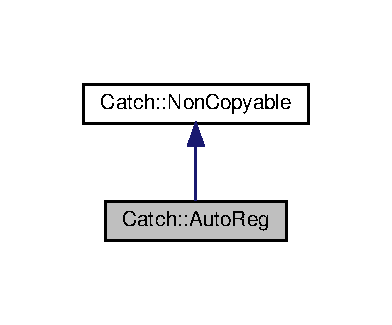
\includegraphics[width=188pt]{structCatch_1_1AutoReg__inherit__graph}
\end{center}
\end{figure}


Collaboration diagram for Catch\+:\+:Auto\+Reg\+:
\nopagebreak
\begin{figure}[H]
\begin{center}
\leavevmode
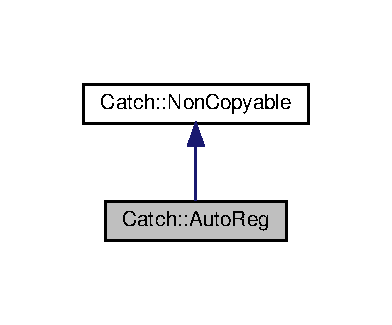
\includegraphics[width=188pt]{structCatch_1_1AutoReg__coll__graph}
\end{center}
\end{figure}
\subsection*{Public Member Functions}
\begin{DoxyCompactItemize}
\item 
\mbox{\Hypertarget{structCatch_1_1AutoReg_a7eba02fb9d80b9896bf5a6517369af28}\label{structCatch_1_1AutoReg_a7eba02fb9d80b9896bf5a6517369af28}} 
{\bfseries Auto\+Reg} (\hyperlink{structCatch_1_1ITestInvoker}{I\+Test\+Invoker} $\ast$invoker, \hyperlink{structCatch_1_1SourceLineInfo}{Source\+Line\+Info} const \&line\+Info, \hyperlink{classCatch_1_1StringRef}{String\+Ref} const \&class\+Or\+Method, \hyperlink{structCatch_1_1NameAndTags}{Name\+And\+Tags} const \&name\+And\+Tags) noexcept
\end{DoxyCompactItemize}


The documentation for this struct was generated from the following file\+:\begin{DoxyCompactItemize}
\item 
/home/sinflair/\+P/crypto/\+A\+K/src/\+Praktikum-\/\+D\+E\+S/catch.\+hpp\end{DoxyCompactItemize}

\hypertarget{classCatch_1_1BinaryExpr}{}\section{Catch\+:\+:Binary\+Expr$<$ LhsT, RhsT $>$ Class Template Reference}
\label{classCatch_1_1BinaryExpr}\index{Catch\+::\+Binary\+Expr$<$ Lhs\+T, Rhs\+T $>$@{Catch\+::\+Binary\+Expr$<$ Lhs\+T, Rhs\+T $>$}}


Inheritance diagram for Catch\+:\+:Binary\+Expr$<$ LhsT, RhsT $>$\+:
\nopagebreak
\begin{figure}[H]
\begin{center}
\leavevmode
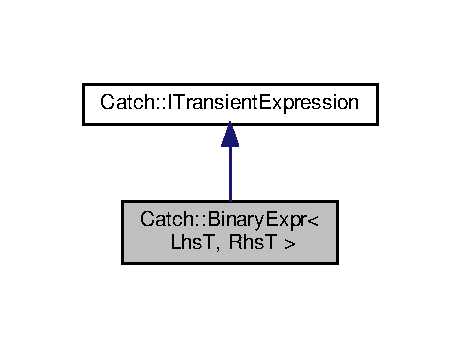
\includegraphics[width=221pt]{classCatch_1_1BinaryExpr__inherit__graph}
\end{center}
\end{figure}


Collaboration diagram for Catch\+:\+:Binary\+Expr$<$ LhsT, RhsT $>$\+:
\nopagebreak
\begin{figure}[H]
\begin{center}
\leavevmode
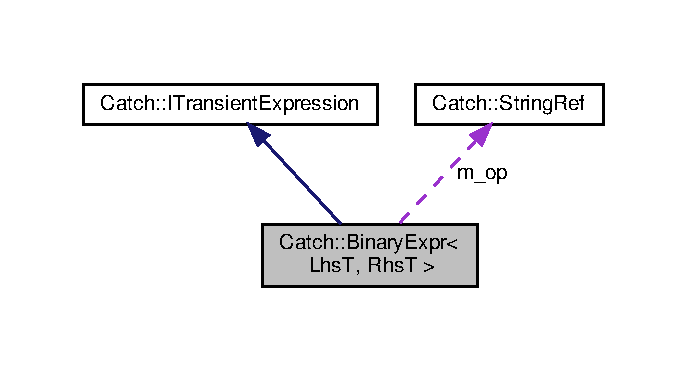
\includegraphics[width=330pt]{classCatch_1_1BinaryExpr__coll__graph}
\end{center}
\end{figure}
\subsection*{Public Member Functions}
\begin{DoxyCompactItemize}
\item 
\mbox{\Hypertarget{classCatch_1_1BinaryExpr_a657d66346aef97a760c22776fe6008b6}\label{classCatch_1_1BinaryExpr_a657d66346aef97a760c22776fe6008b6}} 
{\bfseries Binary\+Expr} (bool comparison\+Result, LhsT lhs, \hyperlink{classCatch_1_1StringRef}{String\+Ref} op, RhsT rhs)
\item 
\mbox{\Hypertarget{classCatch_1_1BinaryExpr_ab51d6e5b8303c5777fd5af916e2fafff}\label{classCatch_1_1BinaryExpr_ab51d6e5b8303c5777fd5af916e2fafff}} 
{\footnotesize template$<$typename T $>$ }\\auto {\bfseries operator\&\&} (T) const -\/$>$ \hyperlink{classCatch_1_1BinaryExpr}{Binary\+Expr}$<$ LhsT, RhsT const \&$>$ const
\item 
\mbox{\Hypertarget{classCatch_1_1BinaryExpr_a44234233ad4fa42e7c95b6a0d94af9db}\label{classCatch_1_1BinaryExpr_a44234233ad4fa42e7c95b6a0d94af9db}} 
{\footnotesize template$<$typename T $>$ }\\auto {\bfseries operator$\vert$$\vert$} (T) const -\/$>$ \hyperlink{classCatch_1_1BinaryExpr}{Binary\+Expr}$<$ LhsT, RhsT const \&$>$ const
\item 
\mbox{\Hypertarget{classCatch_1_1BinaryExpr_a56d7983b7c826c4924423618ffb40e44}\label{classCatch_1_1BinaryExpr_a56d7983b7c826c4924423618ffb40e44}} 
{\footnotesize template$<$typename T $>$ }\\auto {\bfseries operator==} (T) const -\/$>$ \hyperlink{classCatch_1_1BinaryExpr}{Binary\+Expr}$<$ LhsT, RhsT const \&$>$ const
\item 
\mbox{\Hypertarget{classCatch_1_1BinaryExpr_a1c5d4b87cc18452ebe1254e0067dd476}\label{classCatch_1_1BinaryExpr_a1c5d4b87cc18452ebe1254e0067dd476}} 
{\footnotesize template$<$typename T $>$ }\\auto {\bfseries operator!=} (T) const -\/$>$ \hyperlink{classCatch_1_1BinaryExpr}{Binary\+Expr}$<$ LhsT, RhsT const \&$>$ const
\item 
\mbox{\Hypertarget{classCatch_1_1BinaryExpr_a70b66bfaa6df6f8d04e243fda3e0e1e4}\label{classCatch_1_1BinaryExpr_a70b66bfaa6df6f8d04e243fda3e0e1e4}} 
{\footnotesize template$<$typename T $>$ }\\auto {\bfseries operator$>$} (T) const -\/$>$ \hyperlink{classCatch_1_1BinaryExpr}{Binary\+Expr}$<$ LhsT, RhsT const \&$>$ const
\item 
\mbox{\Hypertarget{classCatch_1_1BinaryExpr_a8328cde75134e02d7d44c5277db96c09}\label{classCatch_1_1BinaryExpr_a8328cde75134e02d7d44c5277db96c09}} 
{\footnotesize template$<$typename T $>$ }\\auto {\bfseries operator$<$} (T) const -\/$>$ \hyperlink{classCatch_1_1BinaryExpr}{Binary\+Expr}$<$ LhsT, RhsT const \&$>$ const
\item 
\mbox{\Hypertarget{classCatch_1_1BinaryExpr_a334b84ac38c19c7c961a6d974a6c7d73}\label{classCatch_1_1BinaryExpr_a334b84ac38c19c7c961a6d974a6c7d73}} 
{\footnotesize template$<$typename T $>$ }\\auto {\bfseries operator$>$=} (T) const -\/$>$ \hyperlink{classCatch_1_1BinaryExpr}{Binary\+Expr}$<$ LhsT, RhsT const \&$>$ const
\item 
\mbox{\Hypertarget{classCatch_1_1BinaryExpr_a8773a729df3a465cad4e270e912db436}\label{classCatch_1_1BinaryExpr_a8773a729df3a465cad4e270e912db436}} 
{\footnotesize template$<$typename T $>$ }\\auto {\bfseries operator$<$=} (T) const -\/$>$ \hyperlink{classCatch_1_1BinaryExpr}{Binary\+Expr}$<$ LhsT, RhsT const \&$>$ const
\end{DoxyCompactItemize}
\subsection*{Private Member Functions}
\begin{DoxyCompactItemize}
\item 
\mbox{\Hypertarget{classCatch_1_1BinaryExpr_af998022712d4bd3e4fc7ab9b8a38b445}\label{classCatch_1_1BinaryExpr_af998022712d4bd3e4fc7ab9b8a38b445}} 
void {\bfseries stream\+Reconstructed\+Expression} (std\+::ostream \&os) const override
\end{DoxyCompactItemize}
\subsection*{Private Attributes}
\begin{DoxyCompactItemize}
\item 
\mbox{\Hypertarget{classCatch_1_1BinaryExpr_a306b29e77b48f9c538c5031a59adc4ce}\label{classCatch_1_1BinaryExpr_a306b29e77b48f9c538c5031a59adc4ce}} 
LhsT {\bfseries m\+\_\+lhs}
\item 
\mbox{\Hypertarget{classCatch_1_1BinaryExpr_ab21dea40c53fd64d4f7a073dbe93ec95}\label{classCatch_1_1BinaryExpr_ab21dea40c53fd64d4f7a073dbe93ec95}} 
\hyperlink{classCatch_1_1StringRef}{String\+Ref} {\bfseries m\+\_\+op}
\item 
\mbox{\Hypertarget{classCatch_1_1BinaryExpr_a54cb1629bf304ebe0c1560f4cc2bc186}\label{classCatch_1_1BinaryExpr_a54cb1629bf304ebe0c1560f4cc2bc186}} 
RhsT {\bfseries m\+\_\+rhs}
\end{DoxyCompactItemize}
\subsection*{Additional Inherited Members}


The documentation for this class was generated from the following file\+:\begin{DoxyCompactItemize}
\item 
/home/sinflair/\+P/crypto/\+A\+K/src/\+Praktikum-\/\+D\+E\+S/catch.\+hpp\end{DoxyCompactItemize}

\hypertarget{classBlockCipher}{}\section{Block\+Cipher Class Reference}
\label{classBlockCipher}\index{Block\+Cipher@{Block\+Cipher}}


Inheritance diagram for Block\+Cipher\+:
\nopagebreak
\begin{figure}[H]
\begin{center}
\leavevmode
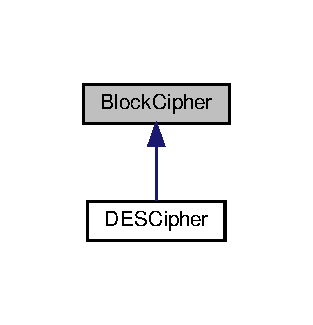
\includegraphics[width=150pt]{classBlockCipher__inherit__graph}
\end{center}
\end{figure}
\subsection*{Public Member Functions}
\begin{DoxyCompactItemize}
\item 
\mbox{\Hypertarget{classBlockCipher_a3c95996f1004e8bbf2b681168d1bd0a9}\label{classBlockCipher_a3c95996f1004e8bbf2b681168d1bd0a9}} 
{\bfseries Block\+Cipher} (unsigned int in\+\_\+block\+\_\+len=8)
\item 
\mbox{\Hypertarget{classBlockCipher_aa6feefe4bf7b8844c44e06240439715a}\label{classBlockCipher_aa6feefe4bf7b8844c44e06240439715a}} 
virtual bool {\bfseries decrypt} (const vector$<$ byte $>$ \&plain\+\_\+text, vector$<$ byte $>$ \&cipher\+\_\+text)=0
\item 
\mbox{\Hypertarget{classBlockCipher_a6b9e82d14004c855a47d79e9de8b3450}\label{classBlockCipher_a6b9e82d14004c855a47d79e9de8b3450}} 
virtual bool {\bfseries encrypt} (const vector$<$ byte $>$ \&plain\+\_\+text, vector$<$ byte $>$ \&cipher\+\_\+text)=0
\item 
\mbox{\Hypertarget{classBlockCipher_a2d97a0cb8efa9109eefea09c7019f064}\label{classBlockCipher_a2d97a0cb8efa9109eefea09c7019f064}} 
virtual bool {\bfseries set\+Key} (const vector$<$ byte $>$ \&key)=0
\end{DoxyCompactItemize}
\subsection*{Static Public Member Functions}
\begin{DoxyCompactItemize}
\item 
\mbox{\Hypertarget{classBlockCipher_ae55a65434bf1d4b59375916a0e58664c}\label{classBlockCipher_ae55a65434bf1d4b59375916a0e58664c}} 
static byte {\bfseries hex\+To\+Byte} (byte xdigit)
\item 
\mbox{\Hypertarget{classBlockCipher_a6c951af389b9ddb9f40c410d18ab5c66}\label{classBlockCipher_a6c951af389b9ddb9f40c410d18ab5c66}} 
static bool {\bfseries read\+Stream} (istream \&strm, vector$<$ byte $>$ \&data, bool hex\+\_\+mode)
\item 
\mbox{\Hypertarget{classBlockCipher_a3839442ae65dd2a710a015b53e9117bf}\label{classBlockCipher_a3839442ae65dd2a710a015b53e9117bf}} 
static void {\bfseries write\+Stream} (ostream \&strm, const vector$<$ byte $>$ \&data, bool hex\+\_\+mode, int columns=30)
\item 
\mbox{\Hypertarget{classBlockCipher_a58dfa6f0548071b3988c8c8990e54c93}\label{classBlockCipher_a58dfa6f0548071b3988c8c8990e54c93}} 
static bool {\bfseries hex\+String\+To\+Vector} (string s, vector$<$ byte $>$ \&data)
\item 
\mbox{\Hypertarget{classBlockCipher_ad000d34ae66e52ee8484a651793d7dfa}\label{classBlockCipher_ad000d34ae66e52ee8484a651793d7dfa}} 
static string {\bfseries to\+Hex\+String} (const vector$<$ byte $>$ \&data)
\end{DoxyCompactItemize}
\subsection*{Protected Attributes}
\begin{DoxyCompactItemize}
\item 
\mbox{\Hypertarget{classBlockCipher_ab29ee03262fd620cd0659e860972faf0}\label{classBlockCipher_ab29ee03262fd620cd0659e860972faf0}} 
unsigned int {\bfseries block\+\_\+len}
\end{DoxyCompactItemize}


The documentation for this class was generated from the following files\+:\begin{DoxyCompactItemize}
\item 
/home/sinflair/\+P/crypto/\+A\+K/src/\+Praktikum-\/\+A\+E\+S/Block\+Cipher.\+h\item 
/home/sinflair/\+P/crypto/\+A\+K/src/\+Praktikum-\/\+A\+E\+S/Block\+Cipher.\+cpp\end{DoxyCompactItemize}

\hypertarget{classCatch_1_1Capturer}{}\section{Catch\+:\+:Capturer Class Reference}
\label{classCatch_1_1Capturer}\index{Catch\+::\+Capturer@{Catch\+::\+Capturer}}


Collaboration diagram for Catch\+:\+:Capturer\+:
\nopagebreak
\begin{figure}[H]
\begin{center}
\leavevmode
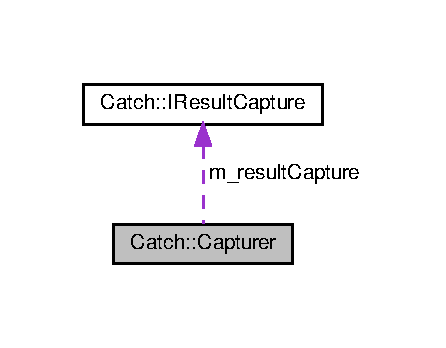
\includegraphics[width=214pt]{classCatch_1_1Capturer__coll__graph}
\end{center}
\end{figure}
\subsection*{Public Member Functions}
\begin{DoxyCompactItemize}
\item 
\mbox{\Hypertarget{classCatch_1_1Capturer_a86b0b27acc803a4e1310c10820f3038f}\label{classCatch_1_1Capturer_a86b0b27acc803a4e1310c10820f3038f}} 
{\bfseries Capturer} (\hyperlink{classCatch_1_1StringRef}{String\+Ref} macro\+Name, \hyperlink{structCatch_1_1SourceLineInfo}{Source\+Line\+Info} const \&line\+Info, Result\+Was\+::\+Of\+Type result\+Type, \hyperlink{classCatch_1_1StringRef}{String\+Ref} names)
\item 
\mbox{\Hypertarget{classCatch_1_1Capturer_a0695ebf77f7cdcb344c73bcb3d9131e4}\label{classCatch_1_1Capturer_a0695ebf77f7cdcb344c73bcb3d9131e4}} 
void {\bfseries capture\+Value} (size\+\_\+t index, std\+::string const \&value)
\item 
\mbox{\Hypertarget{classCatch_1_1Capturer_a60d08e6db2e54740bb2298bbbec3bc0b}\label{classCatch_1_1Capturer_a60d08e6db2e54740bb2298bbbec3bc0b}} 
{\footnotesize template$<$typename T $>$ }\\void {\bfseries capture\+Values} (size\+\_\+t index, T const \&value)
\item 
\mbox{\Hypertarget{classCatch_1_1Capturer_a76f2a097cfeb3042688300b81eb9bcbc}\label{classCatch_1_1Capturer_a76f2a097cfeb3042688300b81eb9bcbc}} 
{\footnotesize template$<$typename T , typename... Ts$>$ }\\void {\bfseries capture\+Values} (size\+\_\+t index, T const \&value, Ts const \&... values)
\end{DoxyCompactItemize}
\subsection*{Private Attributes}
\begin{DoxyCompactItemize}
\item 
\mbox{\Hypertarget{classCatch_1_1Capturer_aefa14693d28906e5e7b06975af38aaed}\label{classCatch_1_1Capturer_aefa14693d28906e5e7b06975af38aaed}} 
std\+::vector$<$ \hyperlink{structCatch_1_1MessageInfo}{Message\+Info} $>$ {\bfseries m\+\_\+messages}
\item 
\mbox{\Hypertarget{classCatch_1_1Capturer_a29edecce81d56837945ba2585c0ff941}\label{classCatch_1_1Capturer_a29edecce81d56837945ba2585c0ff941}} 
\hyperlink{structCatch_1_1IResultCapture}{I\+Result\+Capture} \& {\bfseries m\+\_\+result\+Capture} = get\+Result\+Capture()
\item 
\mbox{\Hypertarget{classCatch_1_1Capturer_a1c3bea0fde97a7663ece4b81187fa9ed}\label{classCatch_1_1Capturer_a1c3bea0fde97a7663ece4b81187fa9ed}} 
size\+\_\+t {\bfseries m\+\_\+captured} = 0
\end{DoxyCompactItemize}


The documentation for this class was generated from the following file\+:\begin{DoxyCompactItemize}
\item 
/home/sinflair/\+P/crypto/\+A\+K/src/\+Praktikum-\/\+D\+E\+S/catch.\+hpp\end{DoxyCompactItemize}

\hypertarget{structCatch_1_1Matchers_1_1StdString_1_1CasedString}{}\section{Catch\+:\+:Matchers\+:\+:Std\+String\+:\+:Cased\+String Struct Reference}
\label{structCatch_1_1Matchers_1_1StdString_1_1CasedString}\index{Catch\+::\+Matchers\+::\+Std\+String\+::\+Cased\+String@{Catch\+::\+Matchers\+::\+Std\+String\+::\+Cased\+String}}
\subsection*{Public Member Functions}
\begin{DoxyCompactItemize}
\item 
\mbox{\Hypertarget{structCatch_1_1Matchers_1_1StdString_1_1CasedString_aa88bbc5acd2bff22351d8d4b1816b561}\label{structCatch_1_1Matchers_1_1StdString_1_1CasedString_aa88bbc5acd2bff22351d8d4b1816b561}} 
{\bfseries Cased\+String} (std\+::string const \&str, Case\+Sensitive\+::\+Choice case\+Sensitivity)
\item 
\mbox{\Hypertarget{structCatch_1_1Matchers_1_1StdString_1_1CasedString_a77639b1165c01f424ee0e96f53335010}\label{structCatch_1_1Matchers_1_1StdString_1_1CasedString_a77639b1165c01f424ee0e96f53335010}} 
std\+::string {\bfseries adjust\+String} (std\+::string const \&str) const
\item 
\mbox{\Hypertarget{structCatch_1_1Matchers_1_1StdString_1_1CasedString_a9759155344d696b2476d764a1d95fcc9}\label{structCatch_1_1Matchers_1_1StdString_1_1CasedString_a9759155344d696b2476d764a1d95fcc9}} 
std\+::string {\bfseries case\+Sensitivity\+Suffix} () const
\end{DoxyCompactItemize}
\subsection*{Public Attributes}
\begin{DoxyCompactItemize}
\item 
\mbox{\Hypertarget{structCatch_1_1Matchers_1_1StdString_1_1CasedString_ae1c2864c986941536a6e94cca0528f92}\label{structCatch_1_1Matchers_1_1StdString_1_1CasedString_ae1c2864c986941536a6e94cca0528f92}} 
Case\+Sensitive\+::\+Choice {\bfseries m\+\_\+case\+Sensitivity}
\item 
\mbox{\Hypertarget{structCatch_1_1Matchers_1_1StdString_1_1CasedString_ad05dbc99aba3c3c386d6b856b213f911}\label{structCatch_1_1Matchers_1_1StdString_1_1CasedString_ad05dbc99aba3c3c386d6b856b213f911}} 
std\+::string {\bfseries m\+\_\+str}
\end{DoxyCompactItemize}


The documentation for this struct was generated from the following file\+:\begin{DoxyCompactItemize}
\item 
/home/sinflair/\+P/crypto/\+A\+K/src/\+Praktikum-\/\+D\+E\+S/catch.\+hpp\end{DoxyCompactItemize}

\hypertarget{structCatch_1_1CaseSensitive}{}\section{Catch\+:\+:Case\+Sensitive Struct Reference}
\label{structCatch_1_1CaseSensitive}\index{Catch\+::\+Case\+Sensitive@{Catch\+::\+Case\+Sensitive}}
\subsection*{Public Types}
\begin{DoxyCompactItemize}
\item 
\mbox{\Hypertarget{structCatch_1_1CaseSensitive_aad49d3aee2d97066642fffa919685c6a}\label{structCatch_1_1CaseSensitive_aad49d3aee2d97066642fffa919685c6a}} 
enum {\bfseries Choice} \{ {\bfseries Yes}, 
{\bfseries No}
 \}
\end{DoxyCompactItemize}


The documentation for this struct was generated from the following file\+:\begin{DoxyCompactItemize}
\item 
/home/sinflair/\+P/crypto/\+A\+K/src/\+Praktikum-\/\+D\+E\+S/catch.\+hpp\end{DoxyCompactItemize}

\hypertarget{structCatch__global__namespace__dummy}{}\section{Catch\+\_\+global\+\_\+namespace\+\_\+dummy Struct Reference}
\label{structCatch__global__namespace__dummy}\index{Catch\+\_\+global\+\_\+namespace\+\_\+dummy@{Catch\+\_\+global\+\_\+namespace\+\_\+dummy}}


The documentation for this struct was generated from the following file\+:\begin{DoxyCompactItemize}
\item 
/home/sinflair/\+P/crypto/\+A\+K/src/\+Praktikum-\/\+D\+E\+S/catch.\+hpp\end{DoxyCompactItemize}

\hypertarget{classCatch_1_1Generators_1_1ChunkGenerator}{}\section{Catch\+:\+:Generators\+:\+:Chunk\+Generator$<$ T $>$ Class Template Reference}
\label{classCatch_1_1Generators_1_1ChunkGenerator}\index{Catch\+::\+Generators\+::\+Chunk\+Generator$<$ T $>$@{Catch\+::\+Generators\+::\+Chunk\+Generator$<$ T $>$}}


Inheritance diagram for Catch\+:\+:Generators\+:\+:Chunk\+Generator$<$ T $>$\+:
\nopagebreak
\begin{figure}[H]
\begin{center}
\leavevmode
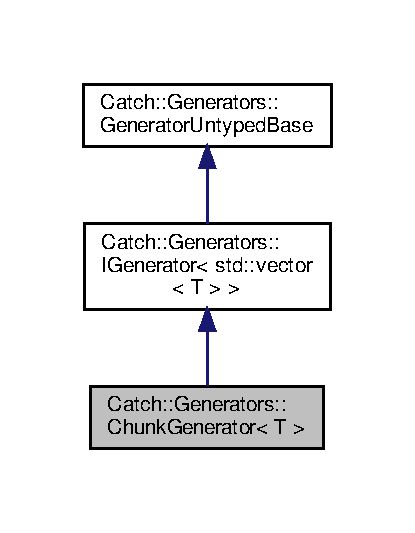
\includegraphics[width=199pt]{classCatch_1_1Generators_1_1ChunkGenerator__inherit__graph}
\end{center}
\end{figure}


Collaboration diagram for Catch\+:\+:Generators\+:\+:Chunk\+Generator$<$ T $>$\+:
\nopagebreak
\begin{figure}[H]
\begin{center}
\leavevmode
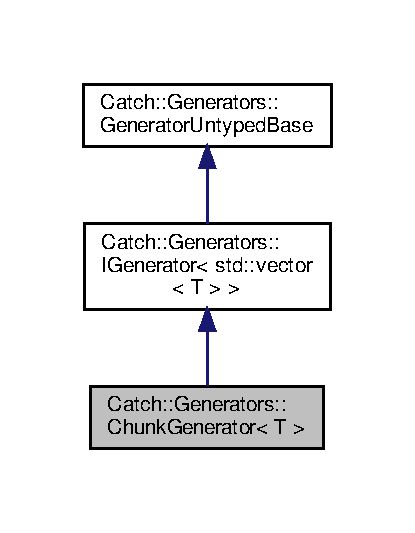
\includegraphics[width=199pt]{classCatch_1_1Generators_1_1ChunkGenerator__coll__graph}
\end{center}
\end{figure}
\subsection*{Public Member Functions}
\begin{DoxyCompactItemize}
\item 
\mbox{\Hypertarget{classCatch_1_1Generators_1_1ChunkGenerator_a50c334d00cde3166d71e9b90ebc2d2e3}\label{classCatch_1_1Generators_1_1ChunkGenerator_a50c334d00cde3166d71e9b90ebc2d2e3}} 
{\bfseries Chunk\+Generator} (size\+\_\+t size, \hyperlink{classCatch_1_1Generators_1_1GeneratorWrapper}{Generator\+Wrapper}$<$ T $>$ generator)
\item 
\mbox{\Hypertarget{classCatch_1_1Generators_1_1ChunkGenerator_aa41c7d08a165b6a18560f2ab9e977f0b}\label{classCatch_1_1Generators_1_1ChunkGenerator_aa41c7d08a165b6a18560f2ab9e977f0b}} 
std\+::vector$<$ T $>$ const  \& {\bfseries get} () const override
\item 
\mbox{\Hypertarget{classCatch_1_1Generators_1_1ChunkGenerator_a545e89f80eb1e3c953491541ea083f86}\label{classCatch_1_1Generators_1_1ChunkGenerator_a545e89f80eb1e3c953491541ea083f86}} 
bool {\bfseries next} () override
\end{DoxyCompactItemize}
\subsection*{Private Attributes}
\begin{DoxyCompactItemize}
\item 
\mbox{\Hypertarget{classCatch_1_1Generators_1_1ChunkGenerator_ab5e382bc5be2e327331bd694a40fa827}\label{classCatch_1_1Generators_1_1ChunkGenerator_ab5e382bc5be2e327331bd694a40fa827}} 
std\+::vector$<$ T $>$ {\bfseries m\+\_\+chunk}
\item 
\mbox{\Hypertarget{classCatch_1_1Generators_1_1ChunkGenerator_a222b9cd460e6d48b12f939833b1b0beb}\label{classCatch_1_1Generators_1_1ChunkGenerator_a222b9cd460e6d48b12f939833b1b0beb}} 
size\+\_\+t {\bfseries m\+\_\+chunk\+\_\+size}
\item 
\mbox{\Hypertarget{classCatch_1_1Generators_1_1ChunkGenerator_aa12b90ee9d029c44528fdba6b9de17bb}\label{classCatch_1_1Generators_1_1ChunkGenerator_aa12b90ee9d029c44528fdba6b9de17bb}} 
\hyperlink{classCatch_1_1Generators_1_1GeneratorWrapper}{Generator\+Wrapper}$<$ T $>$ {\bfseries m\+\_\+generator}
\item 
\mbox{\Hypertarget{classCatch_1_1Generators_1_1ChunkGenerator_a4a5f14d8f6c7a94e5771eb999c1ffe5a}\label{classCatch_1_1Generators_1_1ChunkGenerator_a4a5f14d8f6c7a94e5771eb999c1ffe5a}} 
bool {\bfseries m\+\_\+used\+\_\+up} = false
\end{DoxyCompactItemize}
\subsection*{Additional Inherited Members}


The documentation for this class was generated from the following file\+:\begin{DoxyCompactItemize}
\item 
/home/sinflair/\+P/crypto/\+A\+K/src/\+Praktikum-\/\+D\+E\+S/catch.\+hpp\end{DoxyCompactItemize}

\hypertarget{structcmdline__parser__params}{}\section{cmdline\+\_\+parser\+\_\+params Struct Reference}
\label{structcmdline__parser__params}\index{cmdline\+\_\+parser\+\_\+params@{cmdline\+\_\+parser\+\_\+params}}


The additional parameters to pass to parser functions.  




{\ttfamily \#include $<$aes-\/getopt.\+h$>$}

\subsection*{Public Attributes}
\begin{DoxyCompactItemize}
\item 
\mbox{\Hypertarget{structcmdline__parser__params_ad3ff9d69146e69a47506782197b5675c}\label{structcmdline__parser__params_ad3ff9d69146e69a47506782197b5675c}} 
int \hyperlink{structcmdline__parser__params_ad3ff9d69146e69a47506782197b5675c}{override}
\begin{DoxyCompactList}\small\item\em whether to override possibly already present options (default 0) \end{DoxyCompactList}\item 
\mbox{\Hypertarget{structcmdline__parser__params_a97ed8a6eabd39291ae7d73f273e12c11}\label{structcmdline__parser__params_a97ed8a6eabd39291ae7d73f273e12c11}} 
int \hyperlink{structcmdline__parser__params_a97ed8a6eabd39291ae7d73f273e12c11}{initialize}
\begin{DoxyCompactList}\small\item\em whether to initialize the option structure \hyperlink{structgengetopt__args__info}{gengetopt\+\_\+args\+\_\+info} (default 1) \end{DoxyCompactList}\item 
\mbox{\Hypertarget{structcmdline__parser__params_a44ff439d7e9e36799e59173af74829c6}\label{structcmdline__parser__params_a44ff439d7e9e36799e59173af74829c6}} 
int \hyperlink{structcmdline__parser__params_a44ff439d7e9e36799e59173af74829c6}{check\+\_\+required}
\begin{DoxyCompactList}\small\item\em whether to check that all required options were provided (default 1) \end{DoxyCompactList}\item 
\mbox{\Hypertarget{structcmdline__parser__params_a6e4442704fc40b0b655f7cc602f13ec4}\label{structcmdline__parser__params_a6e4442704fc40b0b655f7cc602f13ec4}} 
int \hyperlink{structcmdline__parser__params_a6e4442704fc40b0b655f7cc602f13ec4}{check\+\_\+ambiguity}
\begin{DoxyCompactList}\small\item\em whether to check for options already specified in the option structure \hyperlink{structgengetopt__args__info}{gengetopt\+\_\+args\+\_\+info} (default 0) \end{DoxyCompactList}\item 
\mbox{\Hypertarget{structcmdline__parser__params_a3236f066777488e8502abe05ccd24455}\label{structcmdline__parser__params_a3236f066777488e8502abe05ccd24455}} 
int \hyperlink{structcmdline__parser__params_a3236f066777488e8502abe05ccd24455}{print\+\_\+errors}
\begin{DoxyCompactList}\small\item\em whether getopt\+\_\+long should print an error message for a bad option (default 1) \end{DoxyCompactList}\end{DoxyCompactItemize}


\subsection{Detailed Description}
The additional parameters to pass to parser functions. 

The documentation for this struct was generated from the following file\+:\begin{DoxyCompactItemize}
\item 
/home/sinflair/\+P/crypto/\+A\+K/src/\+Praktikum-\/\+A\+E\+S/\hyperlink{aes-getopt_8h}{aes-\/getopt.\+h}\end{DoxyCompactItemize}

\hypertarget{structCatch_1_1Matchers_1_1Vector_1_1ContainsElementMatcher}{}\section{Catch\+:\+:Matchers\+:\+:Vector\+:\+:Contains\+Element\+Matcher$<$ T $>$ Struct Template Reference}
\label{structCatch_1_1Matchers_1_1Vector_1_1ContainsElementMatcher}\index{Catch\+::\+Matchers\+::\+Vector\+::\+Contains\+Element\+Matcher$<$ T $>$@{Catch\+::\+Matchers\+::\+Vector\+::\+Contains\+Element\+Matcher$<$ T $>$}}


Inheritance diagram for Catch\+:\+:Matchers\+:\+:Vector\+:\+:Contains\+Element\+Matcher$<$ T $>$\+:
\nopagebreak
\begin{figure}[H]
\begin{center}
\leavevmode
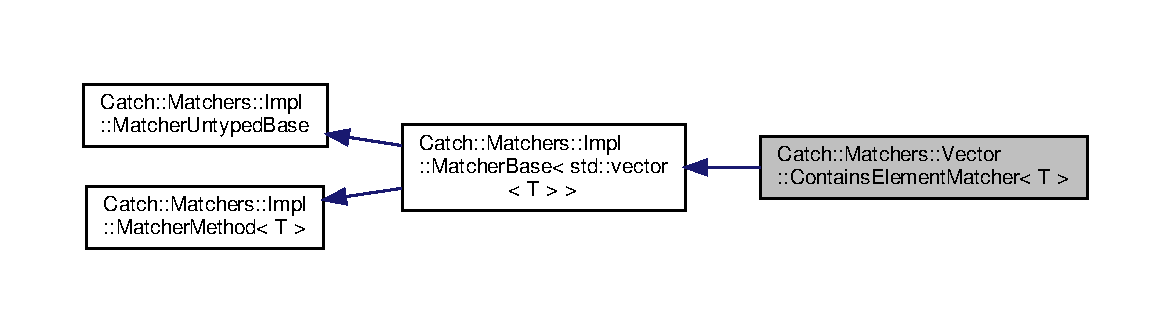
\includegraphics[width=350pt]{structCatch_1_1Matchers_1_1Vector_1_1ContainsElementMatcher__inherit__graph}
\end{center}
\end{figure}


Collaboration diagram for Catch\+:\+:Matchers\+:\+:Vector\+:\+:Contains\+Element\+Matcher$<$ T $>$\+:
\nopagebreak
\begin{figure}[H]
\begin{center}
\leavevmode
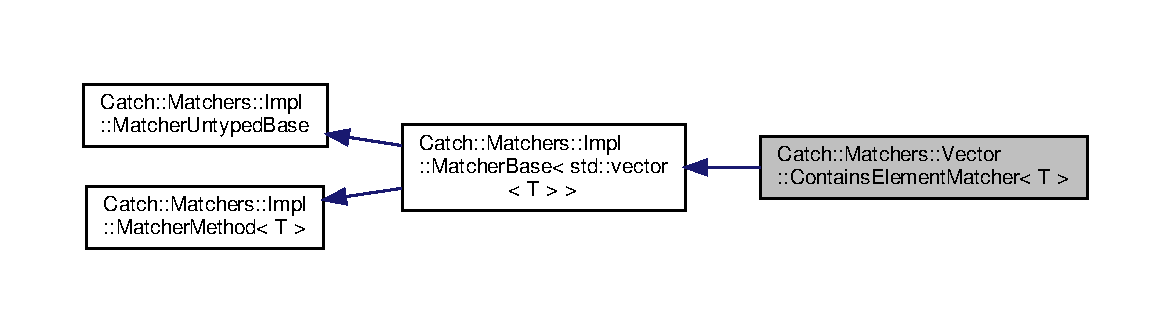
\includegraphics[width=350pt]{structCatch_1_1Matchers_1_1Vector_1_1ContainsElementMatcher__coll__graph}
\end{center}
\end{figure}
\subsection*{Public Member Functions}
\begin{DoxyCompactItemize}
\item 
\mbox{\Hypertarget{structCatch_1_1Matchers_1_1Vector_1_1ContainsElementMatcher_a6a05740b5d3f89fac8de84ac0cff7b93}\label{structCatch_1_1Matchers_1_1Vector_1_1ContainsElementMatcher_a6a05740b5d3f89fac8de84ac0cff7b93}} 
{\bfseries Contains\+Element\+Matcher} (T const \&comparator)
\item 
\mbox{\Hypertarget{structCatch_1_1Matchers_1_1Vector_1_1ContainsElementMatcher_a6a4be6e5642e267433d370649beb0fac}\label{structCatch_1_1Matchers_1_1Vector_1_1ContainsElementMatcher_a6a4be6e5642e267433d370649beb0fac}} 
bool {\bfseries match} (std\+::vector$<$ T $>$ const \&v) const override
\item 
\mbox{\Hypertarget{structCatch_1_1Matchers_1_1Vector_1_1ContainsElementMatcher_aea3b674389a0afd82af6ba4b10f86ae6}\label{structCatch_1_1Matchers_1_1Vector_1_1ContainsElementMatcher_aea3b674389a0afd82af6ba4b10f86ae6}} 
std\+::string {\bfseries describe} () const override
\end{DoxyCompactItemize}
\subsection*{Public Attributes}
\begin{DoxyCompactItemize}
\item 
\mbox{\Hypertarget{structCatch_1_1Matchers_1_1Vector_1_1ContainsElementMatcher_ab7eada6c4bbce1d21b44773262f9cb23}\label{structCatch_1_1Matchers_1_1Vector_1_1ContainsElementMatcher_ab7eada6c4bbce1d21b44773262f9cb23}} 
T const  \& {\bfseries m\+\_\+comparator}
\end{DoxyCompactItemize}
\subsection*{Additional Inherited Members}


The documentation for this struct was generated from the following file\+:\begin{DoxyCompactItemize}
\item 
/home/sinflair/\+P/crypto/\+A\+K/src/\+Praktikum-\/\+D\+E\+S/catch.\+hpp\end{DoxyCompactItemize}

\hypertarget{structCatch_1_1Matchers_1_1StdString_1_1ContainsMatcher}{}\section{Catch\+:\+:Matchers\+:\+:Std\+String\+:\+:Contains\+Matcher Struct Reference}
\label{structCatch_1_1Matchers_1_1StdString_1_1ContainsMatcher}\index{Catch\+::\+Matchers\+::\+Std\+String\+::\+Contains\+Matcher@{Catch\+::\+Matchers\+::\+Std\+String\+::\+Contains\+Matcher}}


Inheritance diagram for Catch\+:\+:Matchers\+:\+:Std\+String\+:\+:Contains\+Matcher\+:
\nopagebreak
\begin{figure}[H]
\begin{center}
\leavevmode
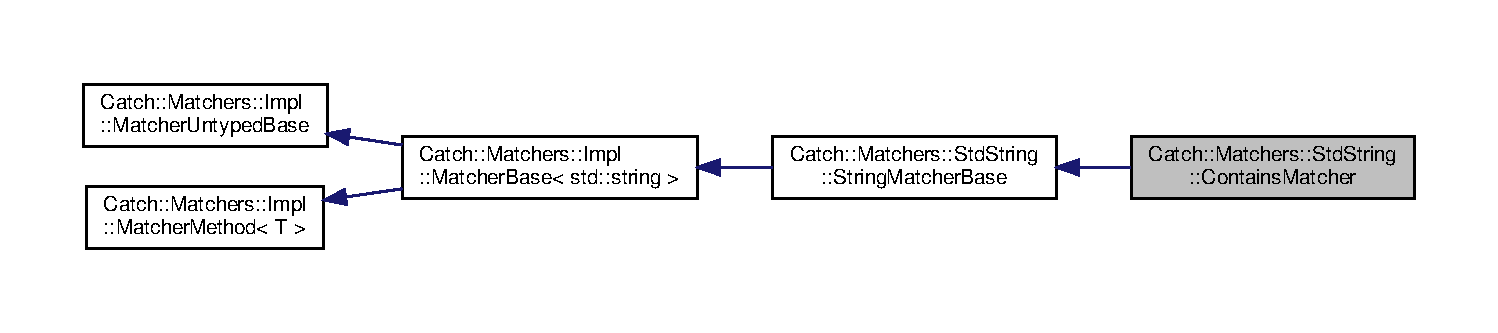
\includegraphics[width=350pt]{structCatch_1_1Matchers_1_1StdString_1_1ContainsMatcher__inherit__graph}
\end{center}
\end{figure}


Collaboration diagram for Catch\+:\+:Matchers\+:\+:Std\+String\+:\+:Contains\+Matcher\+:
\nopagebreak
\begin{figure}[H]
\begin{center}
\leavevmode
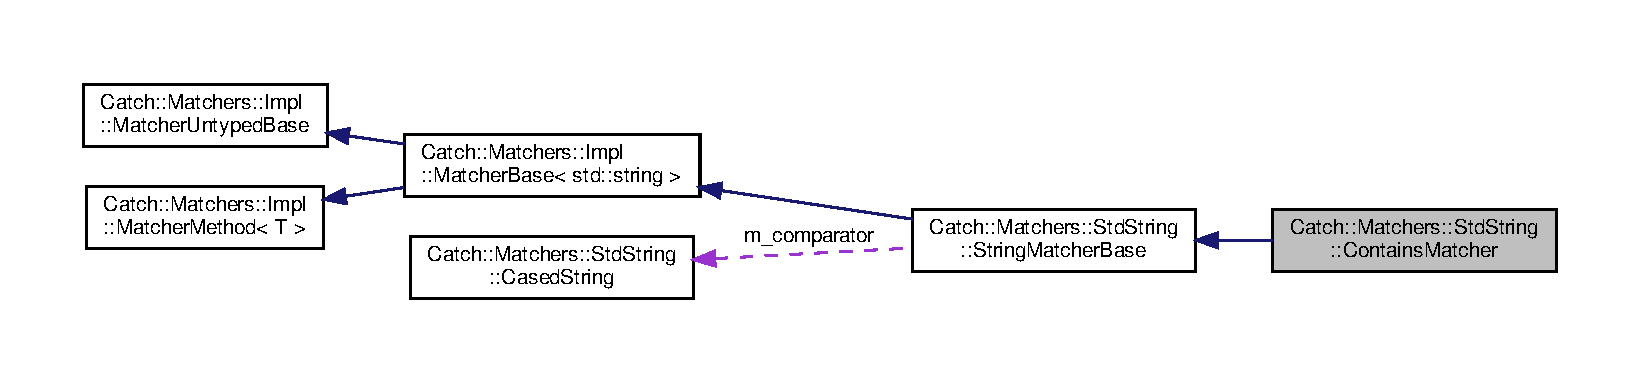
\includegraphics[width=350pt]{structCatch_1_1Matchers_1_1StdString_1_1ContainsMatcher__coll__graph}
\end{center}
\end{figure}
\subsection*{Public Member Functions}
\begin{DoxyCompactItemize}
\item 
\mbox{\Hypertarget{structCatch_1_1Matchers_1_1StdString_1_1ContainsMatcher_acc892883c8409e34b28c9b39d4ef1fe3}\label{structCatch_1_1Matchers_1_1StdString_1_1ContainsMatcher_acc892883c8409e34b28c9b39d4ef1fe3}} 
{\bfseries Contains\+Matcher} (\hyperlink{structCatch_1_1Matchers_1_1StdString_1_1CasedString}{Cased\+String} const \&comparator)
\item 
\mbox{\Hypertarget{structCatch_1_1Matchers_1_1StdString_1_1ContainsMatcher_a630628b234b037be83fe587081a80b53}\label{structCatch_1_1Matchers_1_1StdString_1_1ContainsMatcher_a630628b234b037be83fe587081a80b53}} 
bool {\bfseries match} (std\+::string const \&source) const override
\end{DoxyCompactItemize}
\subsection*{Additional Inherited Members}


The documentation for this struct was generated from the following file\+:\begin{DoxyCompactItemize}
\item 
/home/sinflair/\+P/crypto/\+A\+K/src/\+Praktikum-\/\+D\+E\+S/catch.\+hpp\end{DoxyCompactItemize}

\hypertarget{structCatch_1_1Matchers_1_1Vector_1_1ContainsMatcher}{}\section{Catch\+:\+:Matchers\+:\+:Vector\+:\+:Contains\+Matcher$<$ T $>$ Struct Template Reference}
\label{structCatch_1_1Matchers_1_1Vector_1_1ContainsMatcher}\index{Catch\+::\+Matchers\+::\+Vector\+::\+Contains\+Matcher$<$ T $>$@{Catch\+::\+Matchers\+::\+Vector\+::\+Contains\+Matcher$<$ T $>$}}


Inheritance diagram for Catch\+:\+:Matchers\+:\+:Vector\+:\+:Contains\+Matcher$<$ T $>$\+:
\nopagebreak
\begin{figure}[H]
\begin{center}
\leavevmode
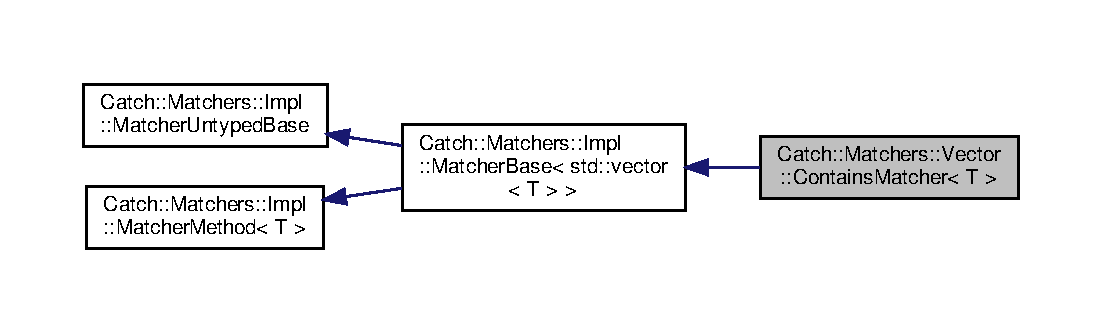
\includegraphics[width=350pt]{structCatch_1_1Matchers_1_1Vector_1_1ContainsMatcher__inherit__graph}
\end{center}
\end{figure}


Collaboration diagram for Catch\+:\+:Matchers\+:\+:Vector\+:\+:Contains\+Matcher$<$ T $>$\+:
\nopagebreak
\begin{figure}[H]
\begin{center}
\leavevmode
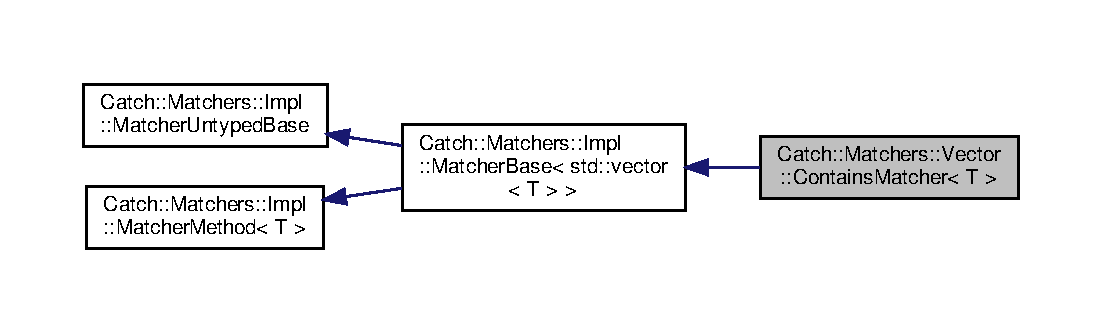
\includegraphics[width=350pt]{structCatch_1_1Matchers_1_1Vector_1_1ContainsMatcher__coll__graph}
\end{center}
\end{figure}
\subsection*{Public Member Functions}
\begin{DoxyCompactItemize}
\item 
\mbox{\Hypertarget{structCatch_1_1Matchers_1_1Vector_1_1ContainsMatcher_ad8e92c8399be6dce75bb5702cdfab700}\label{structCatch_1_1Matchers_1_1Vector_1_1ContainsMatcher_ad8e92c8399be6dce75bb5702cdfab700}} 
{\bfseries Contains\+Matcher} (std\+::vector$<$ T $>$ const \&comparator)
\item 
\mbox{\Hypertarget{structCatch_1_1Matchers_1_1Vector_1_1ContainsMatcher_afd33467ae48a41a634572b41b053f67f}\label{structCatch_1_1Matchers_1_1Vector_1_1ContainsMatcher_afd33467ae48a41a634572b41b053f67f}} 
bool {\bfseries match} (std\+::vector$<$ T $>$ const \&v) const override
\item 
\mbox{\Hypertarget{structCatch_1_1Matchers_1_1Vector_1_1ContainsMatcher_abe6a9ea3d6506c9a1f75ff524f35832e}\label{structCatch_1_1Matchers_1_1Vector_1_1ContainsMatcher_abe6a9ea3d6506c9a1f75ff524f35832e}} 
std\+::string {\bfseries describe} () const override
\end{DoxyCompactItemize}
\subsection*{Public Attributes}
\begin{DoxyCompactItemize}
\item 
\mbox{\Hypertarget{structCatch_1_1Matchers_1_1Vector_1_1ContainsMatcher_a83d051166e4ed0d535219ad6ee99abb2}\label{structCatch_1_1Matchers_1_1Vector_1_1ContainsMatcher_a83d051166e4ed0d535219ad6ee99abb2}} 
std\+::vector$<$ T $>$ const  \& {\bfseries m\+\_\+comparator}
\end{DoxyCompactItemize}
\subsection*{Additional Inherited Members}


The documentation for this struct was generated from the following file\+:\begin{DoxyCompactItemize}
\item 
/home/sinflair/\+P/crypto/\+A\+K/src/\+Praktikum-\/\+D\+E\+S/catch.\+hpp\end{DoxyCompactItemize}

\hypertarget{structCatch_1_1Counts}{}\section{Catch\+:\+:Counts Struct Reference}
\label{structCatch_1_1Counts}\index{Catch\+::\+Counts@{Catch\+::\+Counts}}
\subsection*{Public Member Functions}
\begin{DoxyCompactItemize}
\item 
\mbox{\Hypertarget{structCatch_1_1Counts_aaa10666f559057e3e860d2a5a6fae4c4}\label{structCatch_1_1Counts_aaa10666f559057e3e860d2a5a6fae4c4}} 
\hyperlink{structCatch_1_1Counts}{Counts} {\bfseries operator-\/} (\hyperlink{structCatch_1_1Counts}{Counts} const \&other) const
\item 
\mbox{\Hypertarget{structCatch_1_1Counts_a322a89475cd2cc039140ef371e973677}\label{structCatch_1_1Counts_a322a89475cd2cc039140ef371e973677}} 
\hyperlink{structCatch_1_1Counts}{Counts} \& {\bfseries operator+=} (\hyperlink{structCatch_1_1Counts}{Counts} const \&other)
\item 
\mbox{\Hypertarget{structCatch_1_1Counts_a94f969c09cf52d1339c085c9603cd1d3}\label{structCatch_1_1Counts_a94f969c09cf52d1339c085c9603cd1d3}} 
std\+::size\+\_\+t {\bfseries total} () const
\item 
\mbox{\Hypertarget{structCatch_1_1Counts_a84999490e0ecaa3de5e121bf48eda1b3}\label{structCatch_1_1Counts_a84999490e0ecaa3de5e121bf48eda1b3}} 
bool {\bfseries all\+Passed} () const
\item 
\mbox{\Hypertarget{structCatch_1_1Counts_a33bd996e016030155b99fe1c51c08991}\label{structCatch_1_1Counts_a33bd996e016030155b99fe1c51c08991}} 
bool {\bfseries all\+Ok} () const
\end{DoxyCompactItemize}
\subsection*{Public Attributes}
\begin{DoxyCompactItemize}
\item 
\mbox{\Hypertarget{structCatch_1_1Counts_ad28daaf3de28006400208b6dd0c631e6}\label{structCatch_1_1Counts_ad28daaf3de28006400208b6dd0c631e6}} 
std\+::size\+\_\+t {\bfseries passed} = 0
\item 
\mbox{\Hypertarget{structCatch_1_1Counts_a19982a3817a3bc2c07f0290e71f497a3}\label{structCatch_1_1Counts_a19982a3817a3bc2c07f0290e71f497a3}} 
std\+::size\+\_\+t {\bfseries failed} = 0
\item 
\mbox{\Hypertarget{structCatch_1_1Counts_ac090973a2ff51394cd452718e75c073e}\label{structCatch_1_1Counts_ac090973a2ff51394cd452718e75c073e}} 
std\+::size\+\_\+t {\bfseries failed\+But\+Ok} = 0
\end{DoxyCompactItemize}


The documentation for this struct was generated from the following file\+:\begin{DoxyCompactItemize}
\item 
/home/sinflair/\+P/crypto/\+A\+K/src/\+Praktikum-\/\+D\+E\+S/catch.\+hpp\end{DoxyCompactItemize}

\hypertarget{structcustom__getopt__data}{}\section{custom\+\_\+getopt\+\_\+data Struct Reference}
\label{structcustom__getopt__data}\index{custom\+\_\+getopt\+\_\+data@{custom\+\_\+getopt\+\_\+data}}
\subsection*{Public Attributes}
\begin{DoxyCompactItemize}
\item 
\mbox{\Hypertarget{structcustom__getopt__data_a708838699338a902634d6040f61c9d1e}\label{structcustom__getopt__data_a708838699338a902634d6040f61c9d1e}} 
int {\bfseries custom\+\_\+optind}
\item 
\mbox{\Hypertarget{structcustom__getopt__data_a70368029b9189c6af100d41b95a2a853}\label{structcustom__getopt__data_a70368029b9189c6af100d41b95a2a853}} 
int {\bfseries custom\+\_\+opterr}
\item 
\mbox{\Hypertarget{structcustom__getopt__data_ad986661b4b79755fd55f9f10303221e0}\label{structcustom__getopt__data_ad986661b4b79755fd55f9f10303221e0}} 
int {\bfseries custom\+\_\+optopt}
\item 
\mbox{\Hypertarget{structcustom__getopt__data_a09e50973b9ce49fa0bfa62bb06289f32}\label{structcustom__getopt__data_a09e50973b9ce49fa0bfa62bb06289f32}} 
char $\ast$ {\bfseries custom\+\_\+optarg}
\item 
\mbox{\Hypertarget{structcustom__getopt__data_a5952791becb49374ddfc8726bbf94910}\label{structcustom__getopt__data_a5952791becb49374ddfc8726bbf94910}} 
int {\bfseries initialized}
\item 
\mbox{\Hypertarget{structcustom__getopt__data_a83f042e31dab41b17d8238b528e06121}\label{structcustom__getopt__data_a83f042e31dab41b17d8238b528e06121}} 
char $\ast$ {\bfseries nextchar}
\item 
\mbox{\Hypertarget{structcustom__getopt__data_a89f56362160b74f59aa39d8838dd8bb8}\label{structcustom__getopt__data_a89f56362160b74f59aa39d8838dd8bb8}} 
int {\bfseries first\+\_\+nonopt}
\item 
\mbox{\Hypertarget{structcustom__getopt__data_aff78193409ca6ea017ced550453e0cfd}\label{structcustom__getopt__data_aff78193409ca6ea017ced550453e0cfd}} 
int {\bfseries last\+\_\+nonopt}
\end{DoxyCompactItemize}


The documentation for this struct was generated from the following file\+:\begin{DoxyCompactItemize}
\item 
/home/sinflair/\+P/crypto/\+A\+K/src/\+Praktikum-\/\+A\+E\+S/aes-\/getopt.\+c\end{DoxyCompactItemize}

\hypertarget{structCatch_1_1Decomposer}{}\section{Catch\+:\+:Decomposer Struct Reference}
\label{structCatch_1_1Decomposer}\index{Catch\+::\+Decomposer@{Catch\+::\+Decomposer}}
\subsection*{Public Member Functions}
\begin{DoxyCompactItemize}
\item 
\mbox{\Hypertarget{structCatch_1_1Decomposer_a20b5b8c0e2ff0328a019ae1a8deca03a}\label{structCatch_1_1Decomposer_a20b5b8c0e2ff0328a019ae1a8deca03a}} 
{\footnotesize template$<$typename T $>$ }\\auto {\bfseries operator$<$=} (T const \&lhs) -\/$>$ \hyperlink{classCatch_1_1ExprLhs}{Expr\+Lhs}$<$ T const \&$>$
\item 
\mbox{\Hypertarget{structCatch_1_1Decomposer_aac129b94903ae1339d5709049d83613b}\label{structCatch_1_1Decomposer_aac129b94903ae1339d5709049d83613b}} 
auto {\bfseries operator$<$=} (bool value) -\/$>$ \hyperlink{classCatch_1_1ExprLhs}{Expr\+Lhs}$<$ bool $>$
\end{DoxyCompactItemize}


The documentation for this struct was generated from the following file\+:\begin{DoxyCompactItemize}
\item 
/home/sinflair/\+P/crypto/\+A\+K/src/\+Praktikum-\/\+D\+E\+S/catch.\+hpp\end{DoxyCompactItemize}

\hypertarget{classDESCipher}{}\section{D\+E\+S\+Cipher Class Reference}
\label{classDESCipher}\index{D\+E\+S\+Cipher@{D\+E\+S\+Cipher}}


Inheritance diagram for D\+E\+S\+Cipher\+:
\nopagebreak
\begin{figure}[H]
\begin{center}
\leavevmode
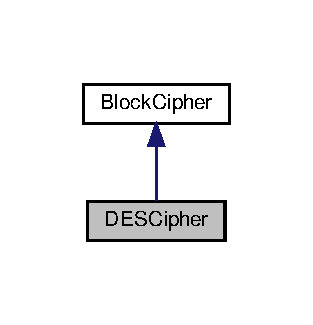
\includegraphics[width=150pt]{classDESCipher__inherit__graph}
\end{center}
\end{figure}


Collaboration diagram for D\+E\+S\+Cipher\+:
\nopagebreak
\begin{figure}[H]
\begin{center}
\leavevmode
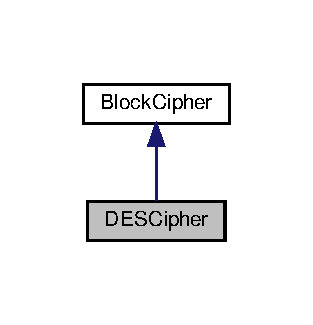
\includegraphics[width=150pt]{classDESCipher__coll__graph}
\end{center}
\end{figure}
\subsection*{Public Member Functions}
\begin{DoxyCompactItemize}
\item 
\hyperlink{classDESCipher_a296b6450dbdf2c35c70c74c628d9176b}{D\+E\+S\+Cipher} ()
\item 
\hyperlink{classDESCipher_ab2a6522ce5c469bfb055e1005ca03fbf}{$\sim$\+D\+E\+S\+Cipher} ()
\item 
void \hyperlink{classDESCipher_a7dc960554f1e80092e62730769b9220b}{compute\+Key\+Schedule} (const byte $\ast$key, bool encmode=true)
\item 
byte \hyperlink{classDESCipher_a5d22aac97342f530e88c8e9cf75908c2}{compute\+S\+Box} (byte id, byte line, byte col)
\item 
virtual int \hyperlink{classDESCipher_a1c4ae4be5ed99cf4278c10742cd09d02}{decrypt} (const byte $\ast$cipher\+\_\+text, int cipher\+\_\+len, const byte $\ast$key, int key\+\_\+len, byte $\ast$plain\+\_\+text, int plain\+\_\+len)
\item 
virtual int \hyperlink{classDESCipher_a61a76488e8087e92ba7f6b827c72db61}{encrypt} (const byte $\ast$plain\+\_\+text, int plain\+\_\+len, const byte $\ast$key, int key\+\_\+len, byte $\ast$cipher\+\_\+text, int cipher\+\_\+len)
\item 
void \hyperlink{classDESCipher_a97f3ae226e5a206ab35c66eef2cd6f75}{process\+Block} (const byte $\ast$in\+\_\+block, byte $\ast$out\+\_\+block)
\item 
void \hyperlink{classDESCipher_a985eafe4c2a27d27289a651ebaedd198}{feistel} (const byte $\ast$l\+\_\+in, const byte $\ast$r\+\_\+in, const byte $\ast$key, byte $\ast$l\+\_\+out, byte $\ast$r\+\_\+out, int rnd=0)
\item 
void \hyperlink{classDESCipher_a1448e493c89acc9d3dd68d1d522dd56b}{functionF} (const byte $\ast$r\+\_\+in, const byte $\ast$key, byte $\ast$r\+\_\+out, int rnd=0)
\item 
bool \hyperlink{classDESCipher_a25226668c299388dfac613b5dc6c3bac}{get\+Bit} (const byte $\ast$array, int array\+\_\+len, int pos) const
\item 
void \hyperlink{classDESCipher_a55e85a3c0fc857b378a1d3a6043ad2bb}{permutate} (const byte $\ast$p, int p\+\_\+len, const byte $\ast$in\+\_\+array, int in\+\_\+len, byte $\ast$out\+\_\+array, int out\+\_\+len) const
\item 
void \hyperlink{classDESCipher_a545d394151b622c2920f634ef2e0b9e2}{print\+Bit\+Field} (const byte $\ast$bytefield, int len, int \hyperlink{classBlockCipher_ab29ee03262fd620cd0659e860972faf0}{block\+\_\+len}=8) const
\item 
void \hyperlink{classDESCipher_aaf4fd9b18be0689fc3c9de0484dfd66c}{set\+Bit} (byte $\ast$array, int array\+\_\+len, int pos, bool value) const
\item 
void \hyperlink{classDESCipher_ace050247cc1d89cf66f85ab890e29a73}{get\+Key\+Schedule} (byte $\ast$key\+Schedule)
\end{DoxyCompactItemize}
\subsection*{Private Attributes}
\begin{DoxyCompactItemize}
\item 
byte \hyperlink{classDESCipher_a15e4c952af35d6b2d19655422b63a54e}{key\+\_\+schedule} \mbox{[}16\mbox{]}\mbox{[}6\mbox{]}
\end{DoxyCompactItemize}
\subsection*{Static Private Attributes}
\begin{DoxyCompactItemize}
\item 
static byte \hyperlink{classDESCipher_aa9e5743835ee06b59c6fad7cf954fde2}{ip} \mbox{[}64\mbox{]}
\item 
static byte \hyperlink{classDESCipher_a4ed481831857615035c294e6a4fcee32}{fp} \mbox{[}64\mbox{]}
\item 
static byte \hyperlink{classDESCipher_a726a2b9846d18e19770eea6d046b3d42}{ev} \mbox{[}48\mbox{]}
\item 
static byte \hyperlink{classDESCipher_acde876e8b143237759022dd47f867945}{pc1} \mbox{[}$\,$\mbox{]}
\item 
static byte \hyperlink{classDESCipher_a16cb4a171e849e673cfaf3d864614e81}{pc2} \mbox{[}$\,$\mbox{]}
\item 
static byte \hyperlink{classDESCipher_af65a5877e08227f4f1817cc6c49dd9bb}{sbox} \mbox{[}8\mbox{]}\mbox{[}64\mbox{]}
\item 
static byte \hyperlink{classDESCipher_af44d8fee3816aeefffd2049697a177cc}{pp} \mbox{[}32\mbox{]}
\item 
static byte \hyperlink{classDESCipher_a28b1d159bad4462f7d89902cd65a8885}{total\+\_\+rot} \mbox{[}16\mbox{]}
\end{DoxyCompactItemize}
\subsection*{Additional Inherited Members}


\subsection{Constructor \& Destructor Documentation}
\mbox{\Hypertarget{classDESCipher_a296b6450dbdf2c35c70c74c628d9176b}\label{classDESCipher_a296b6450dbdf2c35c70c74c628d9176b}} 
\index{D\+E\+S\+Cipher@{D\+E\+S\+Cipher}!D\+E\+S\+Cipher@{D\+E\+S\+Cipher}}
\index{D\+E\+S\+Cipher@{D\+E\+S\+Cipher}!D\+E\+S\+Cipher@{D\+E\+S\+Cipher}}
\subsubsection{\texorpdfstring{D\+E\+S\+Cipher()}{DESCipher()}}
{\footnotesize\ttfamily D\+E\+S\+Cipher\+::\+D\+E\+S\+Cipher (\begin{DoxyParamCaption}{ }\end{DoxyParamCaption})}

Leerer Konstruktor für die \hyperlink{classDESCipher}{D\+E\+S\+Cipher} Klasse \mbox{\Hypertarget{classDESCipher_ab2a6522ce5c469bfb055e1005ca03fbf}\label{classDESCipher_ab2a6522ce5c469bfb055e1005ca03fbf}} 
\index{D\+E\+S\+Cipher@{D\+E\+S\+Cipher}!````~D\+E\+S\+Cipher@{$\sim$\+D\+E\+S\+Cipher}}
\index{````~D\+E\+S\+Cipher@{$\sim$\+D\+E\+S\+Cipher}!D\+E\+S\+Cipher@{D\+E\+S\+Cipher}}
\subsubsection{\texorpdfstring{$\sim$\+D\+E\+S\+Cipher()}{~DESCipher()}}
{\footnotesize\ttfamily D\+E\+S\+Cipher\+::$\sim$\+D\+E\+S\+Cipher (\begin{DoxyParamCaption}{ }\end{DoxyParamCaption})}

Leerer Destruktor für die \hyperlink{classDESCipher}{D\+E\+S\+Cipher} Klasse 

\subsection{Member Function Documentation}
\mbox{\Hypertarget{classDESCipher_a7dc960554f1e80092e62730769b9220b}\label{classDESCipher_a7dc960554f1e80092e62730769b9220b}} 
\index{D\+E\+S\+Cipher@{D\+E\+S\+Cipher}!compute\+Key\+Schedule@{compute\+Key\+Schedule}}
\index{compute\+Key\+Schedule@{compute\+Key\+Schedule}!D\+E\+S\+Cipher@{D\+E\+S\+Cipher}}
\subsubsection{\texorpdfstring{compute\+Key\+Schedule()}{computeKeySchedule()}}
{\footnotesize\ttfamily void D\+E\+S\+Cipher\+::compute\+Key\+Schedule (\begin{DoxyParamCaption}\item[{const byte $\ast$}]{key,  }\item[{bool}]{encmode = {\ttfamily true} }\end{DoxyParamCaption})}

Berechnet die Rundenschlüssel und speichert diese in key\+\_\+schedule ab. Es werden 16 Rundenschlüsselt berechnet, wobei jeder Rundenschlüssel 48 Bit groß ist.


\begin{DoxyParams}{Parameters}
{\em key} & ein konstanter byte Zeiger. Dabei handelt es sich um den 64 Bit großen Schlüssel.\\
\hline
{\em encmode} & gibt an, ob die Rundenschlüssel für das Verschlüsseln (encmode=true) oder das Entschlüsseln (encmode=false) erstellt werden sollen. encmode ist standardmäßig auf true gesetzt. \\
\hline
\end{DoxyParams}
\mbox{\Hypertarget{classDESCipher_a5d22aac97342f530e88c8e9cf75908c2}\label{classDESCipher_a5d22aac97342f530e88c8e9cf75908c2}} 
\index{D\+E\+S\+Cipher@{D\+E\+S\+Cipher}!compute\+S\+Box@{compute\+S\+Box}}
\index{compute\+S\+Box@{compute\+S\+Box}!D\+E\+S\+Cipher@{D\+E\+S\+Cipher}}
\subsubsection{\texorpdfstring{compute\+S\+Box()}{computeSBox()}}
{\footnotesize\ttfamily byte D\+E\+S\+Cipher\+::compute\+S\+Box (\begin{DoxyParamCaption}\item[{byte}]{id,  }\item[{byte}]{line,  }\item[{byte}]{col }\end{DoxyParamCaption})}

compute\+S\+Box liefert ein Arrayelement zurück. Bei dem Array handelt es sich um das sbox 2D Array. Das Element wird über id, line und col bestimmt.

D\+ES verwendet 8 S-\/\+Boxen für Permutationen. Jede S-\/\+Box ist eine nicht lineare Abbildung von \{0,1\}⁶ nach \{0,1\}⁴. Das bedeutet, dass die S-\/\+Box einen 6 Bit Wert auf einen 4 Bit Wert abbildet/zuweist. Der param id gibt an, welche der 8 S-\/\+Boxen verwendet werden soll.

Es gibt 64 verschiedene Werte für \{0,1\}⁶. Jede S-\/\+Box ist deshalb ein 64 Elemente großes Array. Jedes Element ist ein Byte. Da auf \{0,1\}⁴ abgebildet wird, werden nur die unteren 4 Bits des Bytes gesetzt. Die S-\/\+Box kann auch als 4x16 Matrix dargestellt werden. Die ersten 16 Elemente des 64 Elementearrays bilden die erste Zeile der 4x16 Matrix, die darauffolgenden 16 Elemente an Index 16 bis Index 31 des 64 Elementearrays bilden die zweite Zeile der 4x16 Matrix und so weiter. Die param line, die Zeile, und param col, die Spalte, bestimmen das Element Matrix bzw. des 64 Elementearrays.


\begin{DoxyParams}{Parameters}
{\em id} & gibt an, welche S\+Box bzw. welches Array für die Berechnung verwendet werden soll. Es gibt 8 verschiedene S\+Boxen/\+Arrays in sbox. Valide Werte von id sind also 0,1,...,7.\\
\hline
{\em line} & gibt die Zeile der 4x16 S-\/\+Box Matrix an. Da es sich intern um Arrays handelt fängt man hier ab Index 0 an. Valide Werte sind deshalb 0,1,2 und 3.\\
\hline
{\em col} & gibt die Spalte der 4x16 S-\/\+Box Matrix an. Da es sich intern um Arrays handelt fängt man hier ab Index 0 an. Valide Werte sind deshalb 0,1,2,...,15.\\
\hline
\end{DoxyParams}
\begin{DoxyReturn}{Returns}
Der Wert eines Elements der S-\/\+Boxen. Der Rückgabewert ist vom Typ byte, allerdings werden nur die unteren 4 Bits gesetzt sein. 
\end{DoxyReturn}
\mbox{\Hypertarget{classDESCipher_a1c4ae4be5ed99cf4278c10742cd09d02}\label{classDESCipher_a1c4ae4be5ed99cf4278c10742cd09d02}} 
\index{D\+E\+S\+Cipher@{D\+E\+S\+Cipher}!decrypt@{decrypt}}
\index{decrypt@{decrypt}!D\+E\+S\+Cipher@{D\+E\+S\+Cipher}}
\subsubsection{\texorpdfstring{decrypt()}{decrypt()}}
{\footnotesize\ttfamily int D\+E\+S\+Cipher\+::decrypt (\begin{DoxyParamCaption}\item[{const byte $\ast$}]{cipher\+\_\+text,  }\item[{int}]{cipher\+\_\+len,  }\item[{const byte $\ast$}]{key,  }\item[{int}]{key\+\_\+len,  }\item[{byte $\ast$}]{plain\+\_\+text,  }\item[{int}]{plain\+\_\+len }\end{DoxyParamCaption})\hspace{0.3cm}{\ttfamily [virtual]}}

decrypt entschlüsselt cipher\+\_\+len Bytes ab cipher\+\_\+text mit dem key\+\_\+len großen Schlüssel key und speichert den entschlüsselten Text im plain\+\_\+len großen plain\+\_\+text Speicherblock ab.


\begin{DoxyParams}{Parameters}
{\em cipher\+\_\+text} & zeigt auf einen Speicherblock, in dem der mindestens cipher\+\_\+len Byte große verschlüsselte zu entschlüsselnde Text gespeichert ist.\\
\hline
{\em cipher\+\_\+len} & gibt die Größe des cipher\+\_\+text in Byte an. cipher\+\_\+len muss ein vielfaches von der durch \hyperlink{classBlockCipher}{Block\+Cipher} spezifizierten block\+\_\+len sein.\\
\hline
{\em key} & zeigt auf einen Speicherblock, in dem der 8 Byte große Key gespeichert ist. Dieser Key wird für das entschlüsseln verwendet. Speziell werden aus diesem Key die 16 Rundenschlüssel berechnet.\\
\hline
{\em key\+\_\+len} & gibt die Größe des key in Byte an. key\+\_\+len muss gleich 8 sein.\\
\hline
{\em plain\+\_\+text} & zeigt auf einen mindestens plain\+\_\+len großen Speicherblock, in dem der entschlüsselte cipher\+\_\+text gespeichert wird.\\
\hline
{\em plain\+\_\+len} & gibt die Größe des plain\+\_\+text in Byte an. Um das komplette Ergebnis zu speichern muss plain\+\_\+len größer als cipher\+\_\+len sein.\\
\hline
\end{DoxyParams}
\begin{DoxyReturn}{Returns}
den Wert in (param) plain\+\_\+len 
\end{DoxyReturn}


Implements \hyperlink{classBlockCipher_a8a401652231a372a0ec248ff0fb5487a}{Block\+Cipher}.

\mbox{\Hypertarget{classDESCipher_a61a76488e8087e92ba7f6b827c72db61}\label{classDESCipher_a61a76488e8087e92ba7f6b827c72db61}} 
\index{D\+E\+S\+Cipher@{D\+E\+S\+Cipher}!encrypt@{encrypt}}
\index{encrypt@{encrypt}!D\+E\+S\+Cipher@{D\+E\+S\+Cipher}}
\subsubsection{\texorpdfstring{encrypt()}{encrypt()}}
{\footnotesize\ttfamily int D\+E\+S\+Cipher\+::encrypt (\begin{DoxyParamCaption}\item[{const byte $\ast$}]{plain\+\_\+text,  }\item[{int}]{plain\+\_\+len,  }\item[{const byte $\ast$}]{key,  }\item[{int}]{key\+\_\+len,  }\item[{byte $\ast$}]{cipher\+\_\+text,  }\item[{int}]{cipher\+\_\+len }\end{DoxyParamCaption})\hspace{0.3cm}{\ttfamily [virtual]}}

encrypt verschlüsselt plain\+\_\+len Bytes ab plain\+\_\+text mit dem key\+\_\+len großen Schlüssel key und speichert den verschlüsselten Text im cipher\+\_\+len großen cipher\+\_\+text Speicherblock ab.


\begin{DoxyParams}{Parameters}
{\em plain\+\_\+text} & zeigt auf einen Speicherblock, in dem der mindestens plain\+\_\+len Byte große zu verschlüsselnde Text gespeichert ist.\\
\hline
{\em plain\+\_\+len} & gibt die Größe des plain\+\_\+text in Byte an. plain\+\_\+len muss ein vielfaches von der durch \hyperlink{classBlockCipher}{Block\+Cipher} spezifizierten block\+\_\+len sein.\\
\hline
{\em key} & zeigt auf einen Speicherblock, in dem der 8 Byte große Key gespeichert ist. Dieser Key wird für das verschlüsseln verwendet. Mit diesem key kann der resultierende cipher\+\_\+text auch wieder entschlüsselt werden. Speziell werden aus diesem Key die 16 Rundenschlüssel berechnet.\\
\hline
{\em key\+\_\+len} & gibt die Größe des key in Byte an. key\+\_\+len muss gleich 8 sein.\\
\hline
{\em cipher\+\_\+text} & zeigt auf einen mindestens cipher\+\_\+len großen Speicherblock, in dem der verschlüsselte plain\+\_\+text gespeichert wird.\\
\hline
{\em cipher\+\_\+len} & gibt die Größe des cipher\+\_\+text in Byte an. Um das komplette Ergebnis zu speichern muss cipher\+\_\+len größer als plain\+\_\+len sein.\\
\hline
\end{DoxyParams}
\begin{DoxyReturn}{Returns}
den Wert in (param) plain\+\_\+len 
\end{DoxyReturn}


Implements \hyperlink{classBlockCipher_a702dd06a7078ef55c4e9a6482893b07d}{Block\+Cipher}.

\mbox{\Hypertarget{classDESCipher_a985eafe4c2a27d27289a651ebaedd198}\label{classDESCipher_a985eafe4c2a27d27289a651ebaedd198}} 
\index{D\+E\+S\+Cipher@{D\+E\+S\+Cipher}!feistel@{feistel}}
\index{feistel@{feistel}!D\+E\+S\+Cipher@{D\+E\+S\+Cipher}}
\subsubsection{\texorpdfstring{feistel()}{feistel()}}
{\footnotesize\ttfamily void D\+E\+S\+Cipher\+::feistel (\begin{DoxyParamCaption}\item[{const byte $\ast$}]{l\+\_\+in,  }\item[{const byte $\ast$}]{r\+\_\+in,  }\item[{const byte $\ast$}]{key,  }\item[{byte $\ast$}]{l\+\_\+out,  }\item[{byte $\ast$}]{r\+\_\+out,  }\item[{int}]{rnd = {\ttfamily 0} }\end{DoxyParamCaption})}

Implementation der Feistel-\/\+Chiffre. Dabei wird l\+\_\+out auf r\+\_\+in gesetzt. Weiter wird die f Funktion mit r\+\_\+in und key aufgerufen und die Ausgabe der Funktion wird mit l\+\_\+in X\+OR\textquotesingle{}d und in r\+\_\+out geschrieben.


\begin{DoxyParams}{Parameters}
{\em l\+\_\+in} & zeigt auf den 32 Bit großen linken Teil.\\
\hline
{\em r\+\_\+in} & zeigt auf den 32 Bit großen rechten Teil.\\
\hline
{\em key} & zeigt auf einen 48 Bit großen Rundenschlüssel.\\
\hline
{\em l\+\_\+out} & In l\+\_\+out wird der berechnete linke Teil geschrieben.\\
\hline
{\em r\+\_\+out} & In r\+\_\+out wird der berechnete rechte Teil geschrieben. \\
\hline
\end{DoxyParams}
\mbox{\Hypertarget{classDESCipher_a1448e493c89acc9d3dd68d1d522dd56b}\label{classDESCipher_a1448e493c89acc9d3dd68d1d522dd56b}} 
\index{D\+E\+S\+Cipher@{D\+E\+S\+Cipher}!functionF@{functionF}}
\index{functionF@{functionF}!D\+E\+S\+Cipher@{D\+E\+S\+Cipher}}
\subsubsection{\texorpdfstring{function\+F()}{functionF()}}
{\footnotesize\ttfamily void D\+E\+S\+Cipher\+::functionF (\begin{DoxyParamCaption}\item[{const byte $\ast$}]{r\+\_\+in,  }\item[{const byte $\ast$}]{key,  }\item[{byte $\ast$}]{r\+\_\+out,  }\item[{int}]{rnd = {\ttfamily 0} }\end{DoxyParamCaption})}

Implementation der D\+E\+S-\/\+Funktion f. Sie ist eine beliebige injektive Abbildung von \{0, 1\}$^\wedge$(32) × \{0, 1\}$^\wedge$(48) nach \{0, 1\}$^\wedge$(32). Dabei sind r\+\_\+in und key die Eingaben und r\+\_\+out die Ausgabe der Funktion.


\begin{DoxyParams}{Parameters}
{\em r\+\_\+in} & zeigt auf einen 32 Bit großen Speicherblock. Diese 32 Bit werden mit dem Rundenschlüssel key verarbeitet.\\
\hline
{\em key} & zeigt auf einen 48 Bit großen Rundenschlüssel.\\
\hline
{\em r\+\_\+out} & In r\+\_\+out wird die 32 Bit Ausgabe der f Funktion geschrieben.\\
\hline
{\em rnd} & ist optional, gibt die aktuelle D\+ES Runde an und wird in der aktuellen Implementation nicht verwendet. Sie kann in der Zukunft für Debug Ausgaben verwendet werden. \\
\hline
\end{DoxyParams}
\mbox{\Hypertarget{classDESCipher_a25226668c299388dfac613b5dc6c3bac}\label{classDESCipher_a25226668c299388dfac613b5dc6c3bac}} 
\index{D\+E\+S\+Cipher@{D\+E\+S\+Cipher}!get\+Bit@{get\+Bit}}
\index{get\+Bit@{get\+Bit}!D\+E\+S\+Cipher@{D\+E\+S\+Cipher}}
\subsubsection{\texorpdfstring{get\+Bit()}{getBit()}}
{\footnotesize\ttfamily bool D\+E\+S\+Cipher\+::get\+Bit (\begin{DoxyParamCaption}\item[{const byte $\ast$}]{array,  }\item[{int}]{array\+\_\+len,  }\item[{int}]{pos }\end{DoxyParamCaption}) const}

Liefert das pos-\/te Bit des array zurück.


\begin{DoxyParams}{Parameters}
{\em array} & verweist auf einen Speicherblock.\\
\hline
{\em array\+\_\+len} & gibt die Größe des array in Byte an.\\
\hline
{\em pos} & gibt an, dass das pos-\/te Bit zurückgegeben werden soll.\\
\hline
\end{DoxyParams}
\begin{DoxyReturn}{Returns}
den Wert des pos-\/ten Bits des array. 
\end{DoxyReturn}
\mbox{\Hypertarget{classDESCipher_ace050247cc1d89cf66f85ab890e29a73}\label{classDESCipher_ace050247cc1d89cf66f85ab890e29a73}} 
\index{D\+E\+S\+Cipher@{D\+E\+S\+Cipher}!get\+Key\+Schedule@{get\+Key\+Schedule}}
\index{get\+Key\+Schedule@{get\+Key\+Schedule}!D\+E\+S\+Cipher@{D\+E\+S\+Cipher}}
\subsubsection{\texorpdfstring{get\+Key\+Schedule()}{getKeySchedule()}}
{\footnotesize\ttfamily void D\+E\+S\+Cipher\+::get\+Key\+Schedule (\begin{DoxyParamCaption}\item[{byte $\ast$}]{key\+Schedule }\end{DoxyParamCaption})}

get\+Key\+Schedule speichert die 16 6-\/\+Byte großen Rundenschlüssel hintereinander in der durch key\+Schedule gezeigten Position ab. Ab key\+Schedule muss darum 16$\ast$6=96 Byte Speicher reserviert sein.

Zeigt auf einen mindestens 96 Byte großen Speicherblock. In diesen Speicherblock werden die Rundenschlüssel geschrieben. \mbox{\Hypertarget{classDESCipher_a55e85a3c0fc857b378a1d3a6043ad2bb}\label{classDESCipher_a55e85a3c0fc857b378a1d3a6043ad2bb}} 
\index{D\+E\+S\+Cipher@{D\+E\+S\+Cipher}!permutate@{permutate}}
\index{permutate@{permutate}!D\+E\+S\+Cipher@{D\+E\+S\+Cipher}}
\subsubsection{\texorpdfstring{permutate()}{permutate()}}
{\footnotesize\ttfamily void D\+E\+S\+Cipher\+::permutate (\begin{DoxyParamCaption}\item[{const byte $\ast$}]{p,  }\item[{int}]{p\+\_\+len,  }\item[{const byte $\ast$}]{in\+\_\+array,  }\item[{int}]{in\+\_\+len,  }\item[{byte $\ast$}]{out\+\_\+array,  }\item[{int}]{out\+\_\+len }\end{DoxyParamCaption}) const}

p ist ein p\+\_\+len großes Array mit Integern. Die Bits in in\+\_\+array werden an die durch den Wert der Elemente in p bestimmen Position ins out\+\_\+array geschrieben. Das bedeutet, dass das i-\/te Bit in in\+\_\+array an das (p\mbox{[}i\mbox{]}-\/1)-\/te Bit in out\+\_\+array geschrieben, wobei i = 0,1,...,p\+\_\+len-\/1. Die Indices in p starten bei 1 und nicht bei 0.


\begin{DoxyParams}{Parameters}
{\em p} & zeigt auf ein p\+\_\+len byte großes Array, wobei jedes Element des Arrays eine Zuordnung eines Bits auf in\+\_\+array zu out\+\_\+array bestimmt.\\
\hline
{\em p\+\_\+len} & gibt die Größe in byte des p Arrays an.\\
\hline
{\em in\+\_\+array} & zeigt auf ein in\+\_\+len byte großes Array. Bits aus in\+\_\+array werden später an durch p beschriebene Positionen in das out\+\_\+array geschrieben. Es gilt zu beachten, dass möglicherweise keine, manche oder alle Bits aus in\+\_\+array an Positionen in out\+\_\+array kopiert werden und dass auch manche Bits mehrmals in out\+\_\+array kopiert werden können.\\
\hline
{\em in\+\_\+len} & gibt die Größe in bytes des in\+\_\+array an.\\
\hline
{\em out\+\_\+array} & zeigt auf ein out\+\_\+len byte großes Array. Die out\+\_\+len$\ast$8 Bits ab out\+\_\+array werden auf den Wert von Bits des in\+\_\+array gesetzt.\\
\hline
{\em out\+\_\+len} & gibt die Größe in bytes des out\+\_\+array an. \\
\hline
\end{DoxyParams}
\mbox{\Hypertarget{classDESCipher_a545d394151b622c2920f634ef2e0b9e2}\label{classDESCipher_a545d394151b622c2920f634ef2e0b9e2}} 
\index{D\+E\+S\+Cipher@{D\+E\+S\+Cipher}!print\+Bit\+Field@{print\+Bit\+Field}}
\index{print\+Bit\+Field@{print\+Bit\+Field}!D\+E\+S\+Cipher@{D\+E\+S\+Cipher}}
\subsubsection{\texorpdfstring{print\+Bit\+Field()}{printBitField()}}
{\footnotesize\ttfamily void D\+E\+S\+Cipher\+::print\+Bit\+Field (\begin{DoxyParamCaption}\item[{const byte $\ast$}]{bytefield,  }\item[{int}]{len,  }\item[{int}]{block\+\_\+len = {\ttfamily 8} }\end{DoxyParamCaption}) const}

print\+Bit\+Field gibt 8$\ast$len Bit ab bytefield als Bitfolge auf der Standardausgabe aus. Nach jeweils block\+\_\+len bits wird ein Leerzeichen ausgegeben, außer auf das Leerzeichen folgt kein weiteres Bit (no trailing whitespace).


\begin{DoxyParams}{Parameters}
{\em bytefield} & zeigt auf eine Position im Speicher, ab der len Bytes auf der Standardausgabe ausgegeben werden.\\
\hline
{\em len} & gibt die Anzahl der Byte an\\
\hline
{\em block\+\_\+len} & gibt an, nach jeweils wievielen ausgegebenen Bits ein Leerzeichen ausgegeben werden soll. block\+\_\+len ist standardmäßig auf 8 gesetzt. \\
\hline
\end{DoxyParams}
\mbox{\Hypertarget{classDESCipher_a97f3ae226e5a206ab35c66eef2cd6f75}\label{classDESCipher_a97f3ae226e5a206ab35c66eef2cd6f75}} 
\index{D\+E\+S\+Cipher@{D\+E\+S\+Cipher}!process\+Block@{process\+Block}}
\index{process\+Block@{process\+Block}!D\+E\+S\+Cipher@{D\+E\+S\+Cipher}}
\subsubsection{\texorpdfstring{process\+Block()}{processBlock()}}
{\footnotesize\ttfamily void D\+E\+S\+Cipher\+::process\+Block (\begin{DoxyParamCaption}\item[{const byte $\ast$}]{in\+\_\+block,  }\item[{byte $\ast$}]{out\+\_\+block }\end{DoxyParamCaption})}

Chiffriert block\+\_\+len bytes ab in\+\_\+block unter Verwendung der Rundenschlüssel in der Schlüsseltabelle key\+\_\+schedule mittels D\+ES Das Ergebnis wird in den block\+\_\+len bytes ab out\+\_\+block gespeichert. Als Betriebsmodus wird der E\+C\+B-\/\+Modus verwendet.


\begin{DoxyParams}{Parameters}
{\em in\+\_\+block} & zeigt auf die block\+\_\+len Bytes, welche chiffriert werden sollen\\
\hline
{\em out\+\_\+block} & zeigt auf einen Speicherbereich, der mindestens out\+\_\+block Bytes groß sein muss und in welchen das chiffrierte Ergebnis geschrieben wird. \\
\hline
\end{DoxyParams}
\mbox{\Hypertarget{classDESCipher_aaf4fd9b18be0689fc3c9de0484dfd66c}\label{classDESCipher_aaf4fd9b18be0689fc3c9de0484dfd66c}} 
\index{D\+E\+S\+Cipher@{D\+E\+S\+Cipher}!set\+Bit@{set\+Bit}}
\index{set\+Bit@{set\+Bit}!D\+E\+S\+Cipher@{D\+E\+S\+Cipher}}
\subsubsection{\texorpdfstring{set\+Bit()}{setBit()}}
{\footnotesize\ttfamily void D\+E\+S\+Cipher\+::set\+Bit (\begin{DoxyParamCaption}\item[{byte $\ast$}]{array,  }\item[{int}]{array\+\_\+len,  }\item[{int}]{pos,  }\item[{bool}]{value }\end{DoxyParamCaption}) const}

set\+Bit setzt das pos-\/te Bit in array auf den Wert von value.


\begin{DoxyParams}{Parameters}
{\em array} & zeigt auf ein array\+\_\+len Byte großes Feld.\\
\hline
{\em array\+\_\+len} & gibt die Größe des array in Bytes an. Damit das Bit gesetzt werden kann, muss pos $<$ 8$\ast$array\+\_\+len sein.\\
\hline
{\em pos} & gibt an, dass das pos-\/te Bit ab array gesetzt werden soll.\\
\hline
{\em value} & Das pos-\/te Bit wird auf value gesetzt. \\
\hline
\end{DoxyParams}


\subsection{Member Data Documentation}
\mbox{\Hypertarget{classDESCipher_a726a2b9846d18e19770eea6d046b3d42}\label{classDESCipher_a726a2b9846d18e19770eea6d046b3d42}} 
\index{D\+E\+S\+Cipher@{D\+E\+S\+Cipher}!ev@{ev}}
\index{ev@{ev}!D\+E\+S\+Cipher@{D\+E\+S\+Cipher}}
\subsubsection{\texorpdfstring{ev}{ev}}
{\footnotesize\ttfamily byte D\+E\+S\+Cipher\+::ev\hspace{0.3cm}{\ttfamily [static]}, {\ttfamily [private]}}

{\bfseries Initial value\+:}
\begin{DoxyCode}
= \{
        32, 1, 2, 3, 4, 5,
        4, 5, 6, 7, 8, 9,
        8, 9, 10, 11, 12, 13,
        12, 13, 14, 15, 16, 17,
        16, 17, 18, 19, 20, 21,
        20, 21, 22, 23, 24, 25,
        24, 25, 26, 27, 28, 29,
        28, 29, 30, 31, 32, 1
\}
\end{DoxyCode}
ev wird am Anfang der functionF Funktion für die Expansion und Permutation des r\+\_\+in verwendet. \mbox{\Hypertarget{classDESCipher_a4ed481831857615035c294e6a4fcee32}\label{classDESCipher_a4ed481831857615035c294e6a4fcee32}} 
\index{D\+E\+S\+Cipher@{D\+E\+S\+Cipher}!fp@{fp}}
\index{fp@{fp}!D\+E\+S\+Cipher@{D\+E\+S\+Cipher}}
\subsubsection{\texorpdfstring{fp}{fp}}
{\footnotesize\ttfamily byte D\+E\+S\+Cipher\+::fp\hspace{0.3cm}{\ttfamily [static]}, {\ttfamily [private]}}

{\bfseries Initial value\+:}
\begin{DoxyCode}
= \{
        40, 8, 48, 16, 56, 24, 64, 32,
        39, 7, 47, 15, 55, 23, 63, 31,
        38, 6, 46, 14, 54, 22, 62, 30,
        37, 5, 45, 13, 53, 21, 61, 29,
        36, 4, 44, 12, 52, 20, 60, 28,
        35, 3, 43, 11, 51, 19, 59, 27,
        34, 2, 42, 10, 50, 18, 58, 26,
        33, 1, 41, 9, 49, 17, 57, 25
\}
\end{DoxyCode}
fp wird am Ende der process\+Block Funktion für die Permutation des Ergebnis der Rundendurchläufe verwendet. \mbox{\Hypertarget{classDESCipher_aa9e5743835ee06b59c6fad7cf954fde2}\label{classDESCipher_aa9e5743835ee06b59c6fad7cf954fde2}} 
\index{D\+E\+S\+Cipher@{D\+E\+S\+Cipher}!ip@{ip}}
\index{ip@{ip}!D\+E\+S\+Cipher@{D\+E\+S\+Cipher}}
\subsubsection{\texorpdfstring{ip}{ip}}
{\footnotesize\ttfamily byte D\+E\+S\+Cipher\+::ip\hspace{0.3cm}{\ttfamily [static]}, {\ttfamily [private]}}

{\bfseries Initial value\+:}
\begin{DoxyCode}
= \{
        58, 50, 42, 34, 26, 18, 10, 2,
        60, 52, 44, 36, 28, 20, 12, 4,
        62, 54, 46, 38, 30, 22, 14, 6,
        64, 56, 48, 40, 32, 24, 16, 8,
        57, 49, 41, 33, 25, 17, 9, 1,
        59, 51, 43, 35, 27, 19, 11, 3,
        61, 53, 45, 37, 29, 21, 13, 5,
        63, 55, 47, 39, 31, 23, 15, 7
\}
\end{DoxyCode}
ip wird am Anfang der process\+Block Funktion für die Permutation des in\+\_\+block verwendet. \mbox{\Hypertarget{classDESCipher_a15e4c952af35d6b2d19655422b63a54e}\label{classDESCipher_a15e4c952af35d6b2d19655422b63a54e}} 
\index{D\+E\+S\+Cipher@{D\+E\+S\+Cipher}!key\+\_\+schedule@{key\+\_\+schedule}}
\index{key\+\_\+schedule@{key\+\_\+schedule}!D\+E\+S\+Cipher@{D\+E\+S\+Cipher}}
\subsubsection{\texorpdfstring{key\+\_\+schedule}{key\_schedule}}
{\footnotesize\ttfamily byte D\+E\+S\+Cipher\+::key\+\_\+schedule\mbox{[}16\mbox{]}\mbox{[}6\mbox{]}\hspace{0.3cm}{\ttfamily [private]}}

In key\+\_\+schedule werden die 16 6-\/\+Byte großen Rundenschlüssel gespeichert. Die Felder werden von der compute\+Key\+Schedule gesetzt. Jeder Rundenschlüssel wird der Reihe nach über die feistel Funktion an die f Funktion gegeben, um dort zusammen mit dem r\+\_\+in Zustand verarbeitet zu werden.

Das 2D Array kann mit der get\+Key\+Schedule Funktion ausgegeben werden. \mbox{\Hypertarget{classDESCipher_acde876e8b143237759022dd47f867945}\label{classDESCipher_acde876e8b143237759022dd47f867945}} 
\index{D\+E\+S\+Cipher@{D\+E\+S\+Cipher}!pc1@{pc1}}
\index{pc1@{pc1}!D\+E\+S\+Cipher@{D\+E\+S\+Cipher}}
\subsubsection{\texorpdfstring{pc1}{pc1}}
{\footnotesize\ttfamily byte D\+E\+S\+Cipher\+::pc1\hspace{0.3cm}{\ttfamily [static]}, {\ttfamily [private]}}

{\bfseries Initial value\+:}
\begin{DoxyCode}
= \{
        57, 49, 41, 33, 25, 17, 9,
        1, 58, 50, 42, 34, 26, 18,
        10, 2, 59, 51, 43, 35, 27,
        19, 11, 3, 60, 52, 44, 36,

        63, 55, 47, 39, 31, 23, 15,
        7, 62, 54, 46, 38, 30, 22,
        14, 6, 61, 53, 45, 37, 29,
        21, 13, 5, 28, 20, 12, 4
\}
\end{DoxyCode}
pc1 wird in der compute\+Key\+Schedule Funktion verwendet, um für jedes Bit von jedem Rundenschlüssel zu berechnen, welches Bit des Rundenschlüssels auf welches Bit des key gesetzt werden soll. \mbox{\Hypertarget{classDESCipher_a16cb4a171e849e673cfaf3d864614e81}\label{classDESCipher_a16cb4a171e849e673cfaf3d864614e81}} 
\index{D\+E\+S\+Cipher@{D\+E\+S\+Cipher}!pc2@{pc2}}
\index{pc2@{pc2}!D\+E\+S\+Cipher@{D\+E\+S\+Cipher}}
\subsubsection{\texorpdfstring{pc2}{pc2}}
{\footnotesize\ttfamily byte D\+E\+S\+Cipher\+::pc2\hspace{0.3cm}{\ttfamily [static]}, {\ttfamily [private]}}

{\bfseries Initial value\+:}
\begin{DoxyCode}
= \{
        14, 17, 11, 24, 1, 5,
        3, 28, 15, 6, 21, 10,
        23, 19, 12, 4, 26, 8,
        16, 7, 27, 20, 13, 2,
        41, 52, 31, 37, 47, 55,
        30, 40, 51, 45, 33, 48,
        44, 49, 39, 56, 34, 53,
        46, 42, 50, 36, 29, 32
\}
\end{DoxyCode}
pc2 wird wie pc1 in der compute\+Key\+Schedule Funktion verwendet, um für jedes Bit von jedem Rundenschlüssel zu berechnen, welches Bit des Rundenschlüssels auf welches Bit des key gesetzt werden soll. \mbox{\Hypertarget{classDESCipher_af44d8fee3816aeefffd2049697a177cc}\label{classDESCipher_af44d8fee3816aeefffd2049697a177cc}} 
\index{D\+E\+S\+Cipher@{D\+E\+S\+Cipher}!pp@{pp}}
\index{pp@{pp}!D\+E\+S\+Cipher@{D\+E\+S\+Cipher}}
\subsubsection{\texorpdfstring{pp}{pp}}
{\footnotesize\ttfamily byte D\+E\+S\+Cipher\+::pp\hspace{0.3cm}{\ttfamily [static]}, {\ttfamily [private]}}

{\bfseries Initial value\+:}
\begin{DoxyCode}
= \{
        16, 7, 20, 21,
        29, 12, 28, 17,
        1, 15, 23, 26,
        5, 18, 31, 10,
        2, 8, 24, 14,
        32, 27, 3, 9,
        19, 13, 30, 6,
        22, 11, 4, 25
\}
\end{DoxyCode}
pp wird abschließend in der f Funktion für eine Permutation mit dem Ergebnis der S-\/\+Boxen verwendet. Das Ergebnis dieser Permutation wird dann über r\+\_\+out zurückgeliefert. \mbox{\Hypertarget{classDESCipher_af65a5877e08227f4f1817cc6c49dd9bb}\label{classDESCipher_af65a5877e08227f4f1817cc6c49dd9bb}} 
\index{D\+E\+S\+Cipher@{D\+E\+S\+Cipher}!sbox@{sbox}}
\index{sbox@{sbox}!D\+E\+S\+Cipher@{D\+E\+S\+Cipher}}
\subsubsection{\texorpdfstring{sbox}{sbox}}
{\footnotesize\ttfamily byte D\+E\+S\+Cipher\+::sbox\hspace{0.3cm}{\ttfamily [static]}, {\ttfamily [private]}}

Bei sbox handelt es sich um 8 64-\/\+Bit Felder bzw. 8 4x16 Matrizen. Das sind die S-\/\+Boxen, welche über die compute\+S\+Box Funktion für die Permutationen in der f Funktion (functionF) verwendet werden. \mbox{\Hypertarget{classDESCipher_a28b1d159bad4462f7d89902cd65a8885}\label{classDESCipher_a28b1d159bad4462f7d89902cd65a8885}} 
\index{D\+E\+S\+Cipher@{D\+E\+S\+Cipher}!total\+\_\+rot@{total\+\_\+rot}}
\index{total\+\_\+rot@{total\+\_\+rot}!D\+E\+S\+Cipher@{D\+E\+S\+Cipher}}
\subsubsection{\texorpdfstring{total\+\_\+rot}{total\_rot}}
{\footnotesize\ttfamily byte D\+E\+S\+Cipher\+::total\+\_\+rot\hspace{0.3cm}{\ttfamily [static]}, {\ttfamily [private]}}

{\bfseries Initial value\+:}
\begin{DoxyCode}
= \{
        1, 2, 4, 6, 8, 10, 12, 14, 15, 17, 19, 21, 23, 25, 27, 28
\}
\end{DoxyCode}
total\+\_\+rot gibt die Anzahl der zyklischen Linksverschiebungen für jeden Rundenschlüssel an. Das wird in der compute\+Key\+Schedule Funktion verwendet. 

The documentation for this class was generated from the following files\+:\begin{DoxyCompactItemize}
\item 
/home/sinflair/\+P/crypto/\+A\+K/src/\+Praktikum-\/\+D\+E\+S/D\+E\+S\+Cipher.\+h\item 
/home/sinflair/\+P/crypto/\+A\+K/src/\+Praktikum-\/\+D\+E\+S/D\+E\+S\+Cipher.\+cpp\end{DoxyCompactItemize}

\hypertarget{structCatch_1_1Matchers_1_1StdString_1_1EndsWithMatcher}{}\section{Catch\+:\+:Matchers\+:\+:Std\+String\+:\+:Ends\+With\+Matcher Struct Reference}
\label{structCatch_1_1Matchers_1_1StdString_1_1EndsWithMatcher}\index{Catch\+::\+Matchers\+::\+Std\+String\+::\+Ends\+With\+Matcher@{Catch\+::\+Matchers\+::\+Std\+String\+::\+Ends\+With\+Matcher}}


Inheritance diagram for Catch\+:\+:Matchers\+:\+:Std\+String\+:\+:Ends\+With\+Matcher\+:
\nopagebreak
\begin{figure}[H]
\begin{center}
\leavevmode
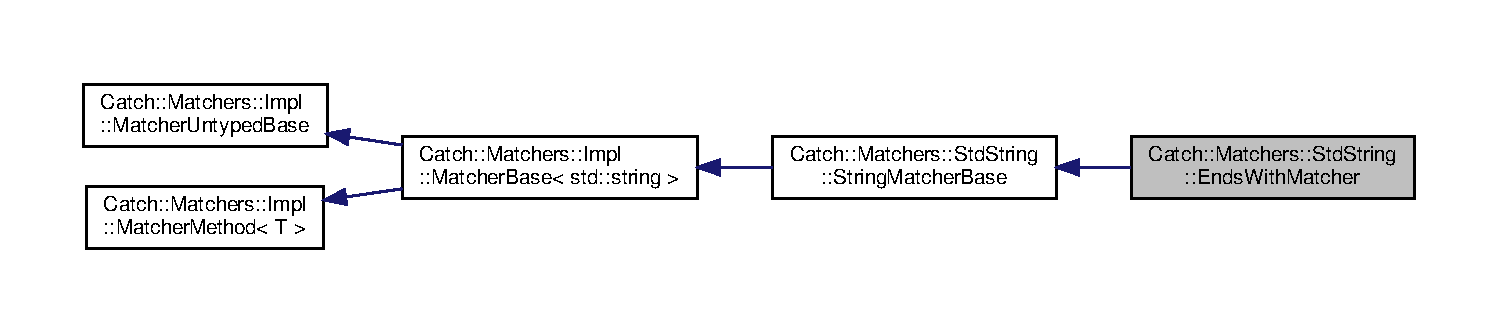
\includegraphics[width=350pt]{structCatch_1_1Matchers_1_1StdString_1_1EndsWithMatcher__inherit__graph}
\end{center}
\end{figure}


Collaboration diagram for Catch\+:\+:Matchers\+:\+:Std\+String\+:\+:Ends\+With\+Matcher\+:
\nopagebreak
\begin{figure}[H]
\begin{center}
\leavevmode
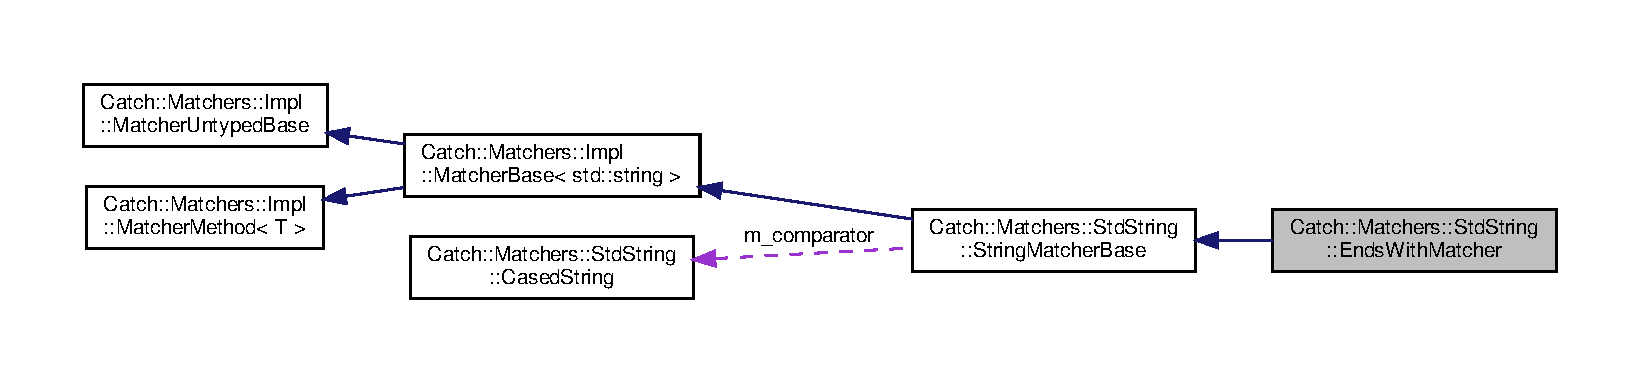
\includegraphics[width=350pt]{structCatch_1_1Matchers_1_1StdString_1_1EndsWithMatcher__coll__graph}
\end{center}
\end{figure}
\subsection*{Public Member Functions}
\begin{DoxyCompactItemize}
\item 
\mbox{\Hypertarget{structCatch_1_1Matchers_1_1StdString_1_1EndsWithMatcher_aa5ec700b4629562f74f362080accfd7b}\label{structCatch_1_1Matchers_1_1StdString_1_1EndsWithMatcher_aa5ec700b4629562f74f362080accfd7b}} 
{\bfseries Ends\+With\+Matcher} (\hyperlink{structCatch_1_1Matchers_1_1StdString_1_1CasedString}{Cased\+String} const \&comparator)
\item 
\mbox{\Hypertarget{structCatch_1_1Matchers_1_1StdString_1_1EndsWithMatcher_aca2741fa57374a2a98d2a84ac3e13a6d}\label{structCatch_1_1Matchers_1_1StdString_1_1EndsWithMatcher_aca2741fa57374a2a98d2a84ac3e13a6d}} 
bool {\bfseries match} (std\+::string const \&source) const override
\end{DoxyCompactItemize}
\subsection*{Additional Inherited Members}


The documentation for this struct was generated from the following file\+:\begin{DoxyCompactItemize}
\item 
/home/sinflair/\+P/crypto/\+A\+K/src/\+Praktikum-\/\+D\+E\+S/catch.\+hpp\end{DoxyCompactItemize}

\hypertarget{structCatch_1_1Detail_1_1EnumInfo}{}\section{Catch\+:\+:Detail\+:\+:Enum\+Info Struct Reference}
\label{structCatch_1_1Detail_1_1EnumInfo}\index{Catch\+::\+Detail\+::\+Enum\+Info@{Catch\+::\+Detail\+::\+Enum\+Info}}


Collaboration diagram for Catch\+:\+:Detail\+:\+:Enum\+Info\+:
\nopagebreak
\begin{figure}[H]
\begin{center}
\leavevmode
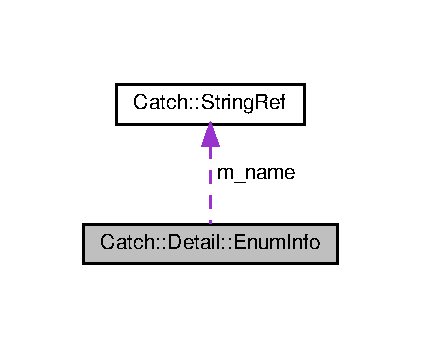
\includegraphics[width=202pt]{structCatch_1_1Detail_1_1EnumInfo__coll__graph}
\end{center}
\end{figure}
\subsection*{Public Member Functions}
\begin{DoxyCompactItemize}
\item 
\mbox{\Hypertarget{structCatch_1_1Detail_1_1EnumInfo_a2fdfacc411d7afb1cb690366e5e49cb3}\label{structCatch_1_1Detail_1_1EnumInfo_a2fdfacc411d7afb1cb690366e5e49cb3}} 
\hyperlink{classCatch_1_1StringRef}{String\+Ref} {\bfseries lookup} (int value) const
\end{DoxyCompactItemize}
\subsection*{Public Attributes}
\begin{DoxyCompactItemize}
\item 
\mbox{\Hypertarget{structCatch_1_1Detail_1_1EnumInfo_a16ecfd3a7e11439433aabbdf6ecb676c}\label{structCatch_1_1Detail_1_1EnumInfo_a16ecfd3a7e11439433aabbdf6ecb676c}} 
\hyperlink{classCatch_1_1StringRef}{String\+Ref} {\bfseries m\+\_\+name}
\item 
\mbox{\Hypertarget{structCatch_1_1Detail_1_1EnumInfo_ad65c0537a50d375859295a2c18ade489}\label{structCatch_1_1Detail_1_1EnumInfo_ad65c0537a50d375859295a2c18ade489}} 
std\+::vector$<$ std\+::pair$<$ int, \hyperlink{classCatch_1_1StringRef}{String\+Ref} $>$ $>$ {\bfseries m\+\_\+values}
\end{DoxyCompactItemize}


The documentation for this struct was generated from the following file\+:\begin{DoxyCompactItemize}
\item 
/home/sinflair/\+P/crypto/\+A\+K/src/\+Praktikum-\/\+D\+E\+S/catch.\+hpp\end{DoxyCompactItemize}

\hypertarget{structCatch_1_1Matchers_1_1StdString_1_1EqualsMatcher}{}\section{Catch\+:\+:Matchers\+:\+:Std\+String\+:\+:Equals\+Matcher Struct Reference}
\label{structCatch_1_1Matchers_1_1StdString_1_1EqualsMatcher}\index{Catch\+::\+Matchers\+::\+Std\+String\+::\+Equals\+Matcher@{Catch\+::\+Matchers\+::\+Std\+String\+::\+Equals\+Matcher}}


Inheritance diagram for Catch\+:\+:Matchers\+:\+:Std\+String\+:\+:Equals\+Matcher\+:
\nopagebreak
\begin{figure}[H]
\begin{center}
\leavevmode
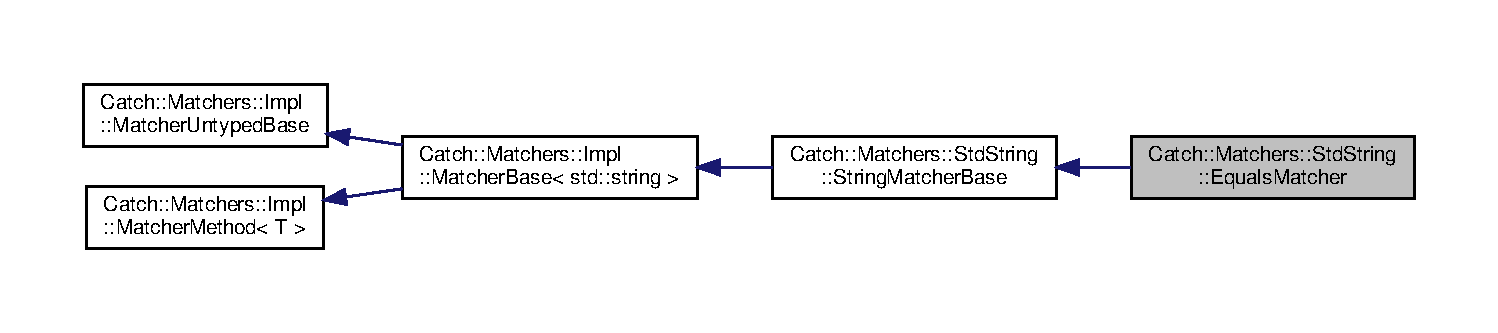
\includegraphics[width=350pt]{structCatch_1_1Matchers_1_1StdString_1_1EqualsMatcher__inherit__graph}
\end{center}
\end{figure}


Collaboration diagram for Catch\+:\+:Matchers\+:\+:Std\+String\+:\+:Equals\+Matcher\+:
\nopagebreak
\begin{figure}[H]
\begin{center}
\leavevmode
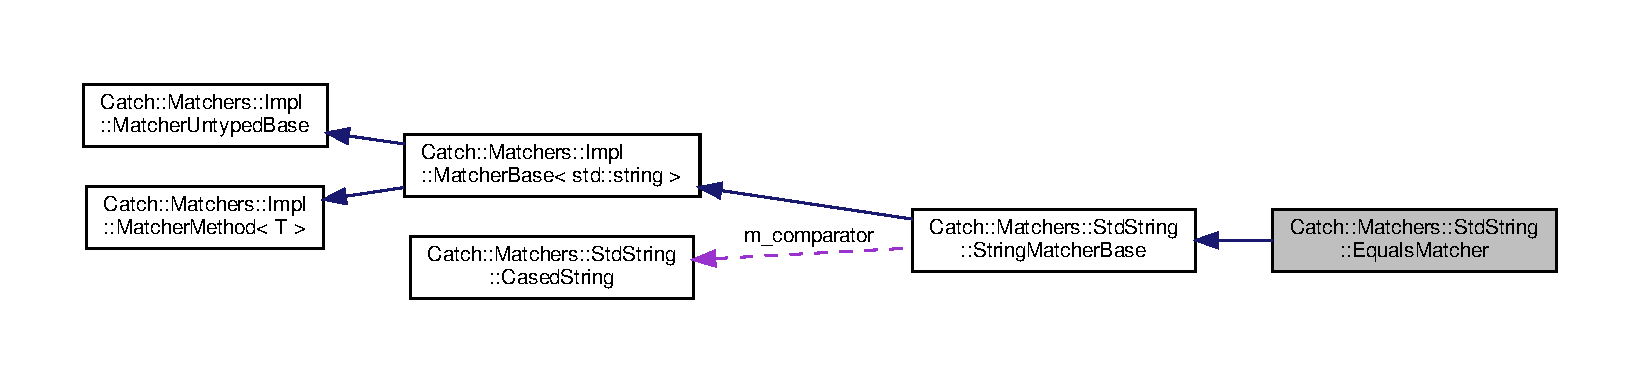
\includegraphics[width=350pt]{structCatch_1_1Matchers_1_1StdString_1_1EqualsMatcher__coll__graph}
\end{center}
\end{figure}
\subsection*{Public Member Functions}
\begin{DoxyCompactItemize}
\item 
\mbox{\Hypertarget{structCatch_1_1Matchers_1_1StdString_1_1EqualsMatcher_ab740f1fb2310e9fe3fed5134d4c7e4c8}\label{structCatch_1_1Matchers_1_1StdString_1_1EqualsMatcher_ab740f1fb2310e9fe3fed5134d4c7e4c8}} 
{\bfseries Equals\+Matcher} (\hyperlink{structCatch_1_1Matchers_1_1StdString_1_1CasedString}{Cased\+String} const \&comparator)
\item 
\mbox{\Hypertarget{structCatch_1_1Matchers_1_1StdString_1_1EqualsMatcher_a0bb9d64693f7bb1ef7441062d219f21a}\label{structCatch_1_1Matchers_1_1StdString_1_1EqualsMatcher_a0bb9d64693f7bb1ef7441062d219f21a}} 
bool {\bfseries match} (std\+::string const \&source) const override
\end{DoxyCompactItemize}
\subsection*{Additional Inherited Members}


The documentation for this struct was generated from the following file\+:\begin{DoxyCompactItemize}
\item 
/home/sinflair/\+P/crypto/\+A\+K/src/\+Praktikum-\/\+D\+E\+S/catch.\+hpp\end{DoxyCompactItemize}

\hypertarget{structCatch_1_1Matchers_1_1Vector_1_1EqualsMatcher}{}\section{Catch\+:\+:Matchers\+:\+:Vector\+:\+:Equals\+Matcher$<$ T $>$ Struct Template Reference}
\label{structCatch_1_1Matchers_1_1Vector_1_1EqualsMatcher}\index{Catch\+::\+Matchers\+::\+Vector\+::\+Equals\+Matcher$<$ T $>$@{Catch\+::\+Matchers\+::\+Vector\+::\+Equals\+Matcher$<$ T $>$}}


Inheritance diagram for Catch\+:\+:Matchers\+:\+:Vector\+:\+:Equals\+Matcher$<$ T $>$\+:
\nopagebreak
\begin{figure}[H]
\begin{center}
\leavevmode
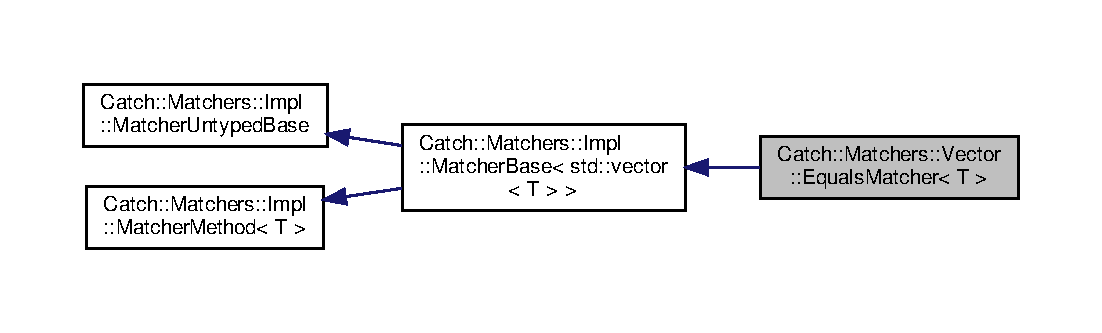
\includegraphics[width=350pt]{structCatch_1_1Matchers_1_1Vector_1_1EqualsMatcher__inherit__graph}
\end{center}
\end{figure}


Collaboration diagram for Catch\+:\+:Matchers\+:\+:Vector\+:\+:Equals\+Matcher$<$ T $>$\+:
\nopagebreak
\begin{figure}[H]
\begin{center}
\leavevmode
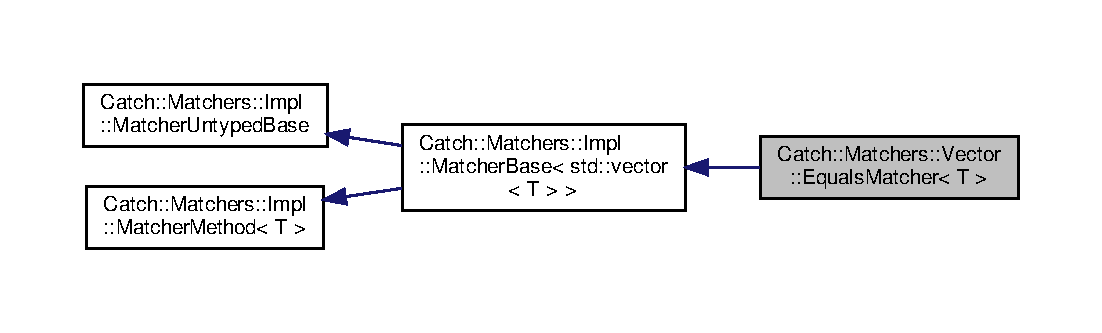
\includegraphics[width=350pt]{structCatch_1_1Matchers_1_1Vector_1_1EqualsMatcher__coll__graph}
\end{center}
\end{figure}
\subsection*{Public Member Functions}
\begin{DoxyCompactItemize}
\item 
\mbox{\Hypertarget{structCatch_1_1Matchers_1_1Vector_1_1EqualsMatcher_a3846c47780d1991dcfe87aefded98008}\label{structCatch_1_1Matchers_1_1Vector_1_1EqualsMatcher_a3846c47780d1991dcfe87aefded98008}} 
{\bfseries Equals\+Matcher} (std\+::vector$<$ T $>$ const \&comparator)
\item 
\mbox{\Hypertarget{structCatch_1_1Matchers_1_1Vector_1_1EqualsMatcher_a2d96cca58a44151fddc5257eda3305da}\label{structCatch_1_1Matchers_1_1Vector_1_1EqualsMatcher_a2d96cca58a44151fddc5257eda3305da}} 
bool {\bfseries match} (std\+::vector$<$ T $>$ const \&v) const override
\item 
\mbox{\Hypertarget{structCatch_1_1Matchers_1_1Vector_1_1EqualsMatcher_a36b5f7ecada4081d6c65bebe8ddea6f4}\label{structCatch_1_1Matchers_1_1Vector_1_1EqualsMatcher_a36b5f7ecada4081d6c65bebe8ddea6f4}} 
std\+::string {\bfseries describe} () const override
\end{DoxyCompactItemize}
\subsection*{Public Attributes}
\begin{DoxyCompactItemize}
\item 
\mbox{\Hypertarget{structCatch_1_1Matchers_1_1Vector_1_1EqualsMatcher_a56f7aa6f110a12b1b9aeb0cabbc9d755}\label{structCatch_1_1Matchers_1_1Vector_1_1EqualsMatcher_a56f7aa6f110a12b1b9aeb0cabbc9d755}} 
std\+::vector$<$ T $>$ const  \& {\bfseries m\+\_\+comparator}
\end{DoxyCompactItemize}
\subsection*{Additional Inherited Members}


The documentation for this struct was generated from the following file\+:\begin{DoxyCompactItemize}
\item 
/home/sinflair/\+P/crypto/\+A\+K/src/\+Praktikum-\/\+D\+E\+S/catch.\+hpp\end{DoxyCompactItemize}

\hypertarget{classCatch_1_1Matchers_1_1Exception_1_1ExceptionMessageMatcher}{}\section{Catch\+:\+:Matchers\+:\+:Exception\+:\+:Exception\+Message\+Matcher Class Reference}
\label{classCatch_1_1Matchers_1_1Exception_1_1ExceptionMessageMatcher}\index{Catch\+::\+Matchers\+::\+Exception\+::\+Exception\+Message\+Matcher@{Catch\+::\+Matchers\+::\+Exception\+::\+Exception\+Message\+Matcher}}


Inheritance diagram for Catch\+:\+:Matchers\+:\+:Exception\+:\+:Exception\+Message\+Matcher\+:
\nopagebreak
\begin{figure}[H]
\begin{center}
\leavevmode
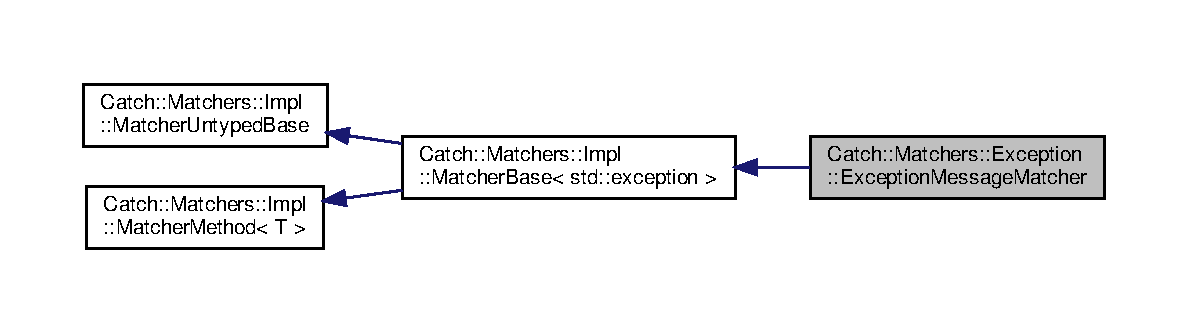
\includegraphics[width=350pt]{classCatch_1_1Matchers_1_1Exception_1_1ExceptionMessageMatcher__inherit__graph}
\end{center}
\end{figure}


Collaboration diagram for Catch\+:\+:Matchers\+:\+:Exception\+:\+:Exception\+Message\+Matcher\+:
\nopagebreak
\begin{figure}[H]
\begin{center}
\leavevmode
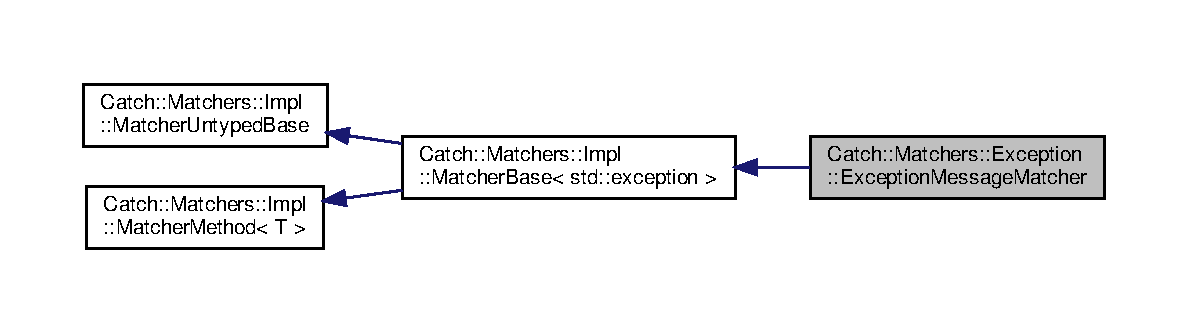
\includegraphics[width=350pt]{classCatch_1_1Matchers_1_1Exception_1_1ExceptionMessageMatcher__coll__graph}
\end{center}
\end{figure}
\subsection*{Public Member Functions}
\begin{DoxyCompactItemize}
\item 
\mbox{\Hypertarget{classCatch_1_1Matchers_1_1Exception_1_1ExceptionMessageMatcher_ace55942f39ba653db3fd69d6d90e188f}\label{classCatch_1_1Matchers_1_1Exception_1_1ExceptionMessageMatcher_ace55942f39ba653db3fd69d6d90e188f}} 
{\bfseries Exception\+Message\+Matcher} (std\+::string const \&message)
\item 
\mbox{\Hypertarget{classCatch_1_1Matchers_1_1Exception_1_1ExceptionMessageMatcher_aa0566d24990d69e96495360b8f79593d}\label{classCatch_1_1Matchers_1_1Exception_1_1ExceptionMessageMatcher_aa0566d24990d69e96495360b8f79593d}} 
bool {\bfseries match} (std\+::exception const \&ex) const override
\item 
\mbox{\Hypertarget{classCatch_1_1Matchers_1_1Exception_1_1ExceptionMessageMatcher_a3543441985ec877a781e660a403b1bae}\label{classCatch_1_1Matchers_1_1Exception_1_1ExceptionMessageMatcher_a3543441985ec877a781e660a403b1bae}} 
std\+::string {\bfseries describe} () const override
\end{DoxyCompactItemize}
\subsection*{Private Attributes}
\begin{DoxyCompactItemize}
\item 
\mbox{\Hypertarget{classCatch_1_1Matchers_1_1Exception_1_1ExceptionMessageMatcher_a1cf4836834c357febac9180ab74a178a}\label{classCatch_1_1Matchers_1_1Exception_1_1ExceptionMessageMatcher_a1cf4836834c357febac9180ab74a178a}} 
std\+::string {\bfseries m\+\_\+message}
\end{DoxyCompactItemize}
\subsection*{Additional Inherited Members}


The documentation for this class was generated from the following file\+:\begin{DoxyCompactItemize}
\item 
/home/sinflair/\+P/crypto/\+A\+K/src/\+Praktikum-\/\+D\+E\+S/catch.\+hpp\end{DoxyCompactItemize}

\hypertarget{classCatch_1_1ExceptionTranslatorRegistrar_1_1ExceptionTranslator}{}\section{Catch\+:\+:Exception\+Translator\+Registrar\+:\+:Exception\+Translator$<$ T $>$ Class Template Reference}
\label{classCatch_1_1ExceptionTranslatorRegistrar_1_1ExceptionTranslator}\index{Catch\+::\+Exception\+Translator\+Registrar\+::\+Exception\+Translator$<$ T $>$@{Catch\+::\+Exception\+Translator\+Registrar\+::\+Exception\+Translator$<$ T $>$}}


Inheritance diagram for Catch\+:\+:Exception\+Translator\+Registrar\+:\+:Exception\+Translator$<$ T $>$\+:
\nopagebreak
\begin{figure}[H]
\begin{center}
\leavevmode
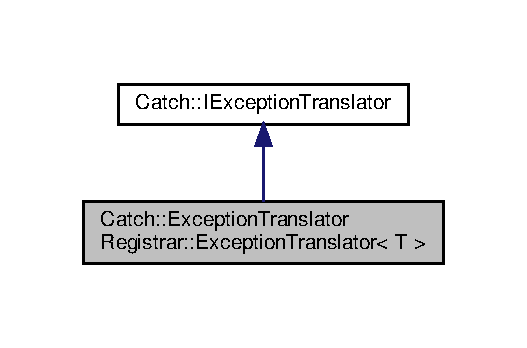
\includegraphics[width=253pt]{classCatch_1_1ExceptionTranslatorRegistrar_1_1ExceptionTranslator__inherit__graph}
\end{center}
\end{figure}


Collaboration diagram for Catch\+:\+:Exception\+Translator\+Registrar\+:\+:Exception\+Translator$<$ T $>$\+:
\nopagebreak
\begin{figure}[H]
\begin{center}
\leavevmode
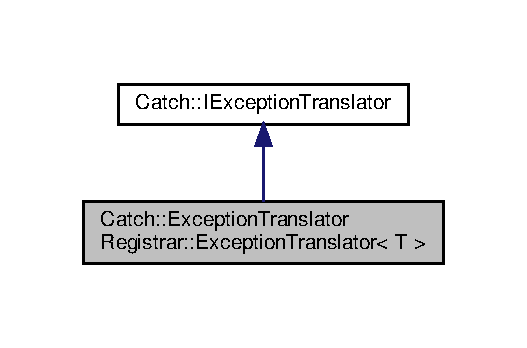
\includegraphics[width=253pt]{classCatch_1_1ExceptionTranslatorRegistrar_1_1ExceptionTranslator__coll__graph}
\end{center}
\end{figure}
\subsection*{Public Member Functions}
\begin{DoxyCompactItemize}
\item 
\mbox{\Hypertarget{classCatch_1_1ExceptionTranslatorRegistrar_1_1ExceptionTranslator_a2de4e9bcaad47996159763e69f614d7a}\label{classCatch_1_1ExceptionTranslatorRegistrar_1_1ExceptionTranslator_a2de4e9bcaad47996159763e69f614d7a}} 
{\bfseries Exception\+Translator} (std\+::string($\ast$translate\+Function)(T \&))
\item 
\mbox{\Hypertarget{classCatch_1_1ExceptionTranslatorRegistrar_1_1ExceptionTranslator_a29e85940ee9ce719f26e43550cb4ed48}\label{classCatch_1_1ExceptionTranslatorRegistrar_1_1ExceptionTranslator_a29e85940ee9ce719f26e43550cb4ed48}} 
std\+::string {\bfseries translate} (Exception\+Translators\+::const\+\_\+iterator it, Exception\+Translators\+::const\+\_\+iterator it\+End) const override
\end{DoxyCompactItemize}
\subsection*{Protected Attributes}
\begin{DoxyCompactItemize}
\item 
\mbox{\Hypertarget{classCatch_1_1ExceptionTranslatorRegistrar_1_1ExceptionTranslator_a488013ff0869785c9d041443fbf9a757}\label{classCatch_1_1ExceptionTranslatorRegistrar_1_1ExceptionTranslator_a488013ff0869785c9d041443fbf9a757}} 
std\+::string($\ast$ {\bfseries m\+\_\+translate\+Function} )(T \&)
\end{DoxyCompactItemize}


The documentation for this class was generated from the following file\+:\begin{DoxyCompactItemize}
\item 
/home/sinflair/\+P/crypto/\+A\+K/src/\+Praktikum-\/\+D\+E\+S/catch.\+hpp\end{DoxyCompactItemize}

\hypertarget{classCatch_1_1ExceptionTranslatorRegistrar}{}\section{Catch\+:\+:Exception\+Translator\+Registrar Class Reference}
\label{classCatch_1_1ExceptionTranslatorRegistrar}\index{Catch\+::\+Exception\+Translator\+Registrar@{Catch\+::\+Exception\+Translator\+Registrar}}
\subsection*{Classes}
\begin{DoxyCompactItemize}
\item 
class \hyperlink{classCatch_1_1ExceptionTranslatorRegistrar_1_1ExceptionTranslator}{Exception\+Translator}
\end{DoxyCompactItemize}
\subsection*{Public Member Functions}
\begin{DoxyCompactItemize}
\item 
\mbox{\Hypertarget{classCatch_1_1ExceptionTranslatorRegistrar_aa73229de911f26b1df6c6c87c4d9e04e}\label{classCatch_1_1ExceptionTranslatorRegistrar_aa73229de911f26b1df6c6c87c4d9e04e}} 
{\footnotesize template$<$typename T $>$ }\\{\bfseries Exception\+Translator\+Registrar} (std\+::string($\ast$translate\+Function)(T \&))
\end{DoxyCompactItemize}


The documentation for this class was generated from the following file\+:\begin{DoxyCompactItemize}
\item 
/home/sinflair/\+P/crypto/\+A\+K/src/\+Praktikum-\/\+D\+E\+S/catch.\+hpp\end{DoxyCompactItemize}

\hypertarget{classCatch_1_1ExprLhs}{}\section{Catch\+:\+:Expr\+Lhs$<$ LhsT $>$ Class Template Reference}
\label{classCatch_1_1ExprLhs}\index{Catch\+::\+Expr\+Lhs$<$ Lhs\+T $>$@{Catch\+::\+Expr\+Lhs$<$ Lhs\+T $>$}}
\subsection*{Public Member Functions}
\begin{DoxyCompactItemize}
\item 
\mbox{\Hypertarget{classCatch_1_1ExprLhs_ad22c6af1a7d6993240624d299714a479}\label{classCatch_1_1ExprLhs_ad22c6af1a7d6993240624d299714a479}} 
{\bfseries Expr\+Lhs} (LhsT lhs)
\item 
\mbox{\Hypertarget{classCatch_1_1ExprLhs_a3068adff1dbbaeec62ffc368d4d6cc4d}\label{classCatch_1_1ExprLhs_a3068adff1dbbaeec62ffc368d4d6cc4d}} 
{\footnotesize template$<$typename RhsT $>$ }\\auto {\bfseries operator==} (RhsT const \&rhs) -\/$>$ \hyperlink{classCatch_1_1BinaryExpr}{Binary\+Expr}$<$ LhsT, RhsT const \&$>$ const
\item 
\mbox{\Hypertarget{classCatch_1_1ExprLhs_ab707a84abdffbdc35962a495e238d393}\label{classCatch_1_1ExprLhs_ab707a84abdffbdc35962a495e238d393}} 
auto {\bfseries operator==} (bool rhs) -\/$>$ \hyperlink{classCatch_1_1BinaryExpr}{Binary\+Expr}$<$ LhsT, bool $>$ const
\item 
\mbox{\Hypertarget{classCatch_1_1ExprLhs_a5e10eab8aed53dd000b89d8fd7754437}\label{classCatch_1_1ExprLhs_a5e10eab8aed53dd000b89d8fd7754437}} 
{\footnotesize template$<$typename RhsT $>$ }\\auto {\bfseries operator!=} (RhsT const \&rhs) -\/$>$ \hyperlink{classCatch_1_1BinaryExpr}{Binary\+Expr}$<$ LhsT, RhsT const \&$>$ const
\item 
\mbox{\Hypertarget{classCatch_1_1ExprLhs_a60eca847201d057d8a8b7222c69b619c}\label{classCatch_1_1ExprLhs_a60eca847201d057d8a8b7222c69b619c}} 
auto {\bfseries operator!=} (bool rhs) -\/$>$ \hyperlink{classCatch_1_1BinaryExpr}{Binary\+Expr}$<$ LhsT, bool $>$ const
\item 
\mbox{\Hypertarget{classCatch_1_1ExprLhs_a23cb0cd983a1ac9c3df5160542199b83}\label{classCatch_1_1ExprLhs_a23cb0cd983a1ac9c3df5160542199b83}} 
{\footnotesize template$<$typename RhsT $>$ }\\auto {\bfseries operator$>$} (RhsT const \&rhs) -\/$>$ \hyperlink{classCatch_1_1BinaryExpr}{Binary\+Expr}$<$ LhsT, RhsT const \&$>$ const
\item 
\mbox{\Hypertarget{classCatch_1_1ExprLhs_a55284221df2edb3542e765c87b5691b9}\label{classCatch_1_1ExprLhs_a55284221df2edb3542e765c87b5691b9}} 
{\footnotesize template$<$typename RhsT $>$ }\\auto {\bfseries operator$<$} (RhsT const \&rhs) -\/$>$ \hyperlink{classCatch_1_1BinaryExpr}{Binary\+Expr}$<$ LhsT, RhsT const \&$>$ const
\item 
\mbox{\Hypertarget{classCatch_1_1ExprLhs_aff594ae5b957105c517a6257d2e730f0}\label{classCatch_1_1ExprLhs_aff594ae5b957105c517a6257d2e730f0}} 
{\footnotesize template$<$typename RhsT $>$ }\\auto {\bfseries operator$>$=} (RhsT const \&rhs) -\/$>$ \hyperlink{classCatch_1_1BinaryExpr}{Binary\+Expr}$<$ LhsT, RhsT const \&$>$ const
\item 
\mbox{\Hypertarget{classCatch_1_1ExprLhs_a6bd8a22c1a7fe2f66d71d7196f20af4f}\label{classCatch_1_1ExprLhs_a6bd8a22c1a7fe2f66d71d7196f20af4f}} 
{\footnotesize template$<$typename RhsT $>$ }\\auto {\bfseries operator$<$=} (RhsT const \&rhs) -\/$>$ \hyperlink{classCatch_1_1BinaryExpr}{Binary\+Expr}$<$ LhsT, RhsT const \&$>$ const
\item 
\mbox{\Hypertarget{classCatch_1_1ExprLhs_a5d85cdd34a136c37fa5e5283c2ff54d5}\label{classCatch_1_1ExprLhs_a5d85cdd34a136c37fa5e5283c2ff54d5}} 
{\footnotesize template$<$typename RhsT $>$ }\\auto {\bfseries operator\&\&} (RhsT const \&) -\/$>$ \hyperlink{classCatch_1_1BinaryExpr}{Binary\+Expr}$<$ LhsT, RhsT const \&$>$ const
\item 
\mbox{\Hypertarget{classCatch_1_1ExprLhs_a33e5f813f5c236b9b77d977c04266f4d}\label{classCatch_1_1ExprLhs_a33e5f813f5c236b9b77d977c04266f4d}} 
{\footnotesize template$<$typename RhsT $>$ }\\auto {\bfseries operator$\vert$$\vert$} (RhsT const \&) -\/$>$ \hyperlink{classCatch_1_1BinaryExpr}{Binary\+Expr}$<$ LhsT, RhsT const \&$>$ const
\item 
\mbox{\Hypertarget{classCatch_1_1ExprLhs_ab68bd6d5d3ae21b7fba9010150fba95d}\label{classCatch_1_1ExprLhs_ab68bd6d5d3ae21b7fba9010150fba95d}} 
auto {\bfseries make\+Unary\+Expr} () const -\/$>$ \hyperlink{classCatch_1_1UnaryExpr}{Unary\+Expr}$<$ LhsT $>$
\end{DoxyCompactItemize}
\subsection*{Private Attributes}
\begin{DoxyCompactItemize}
\item 
\mbox{\Hypertarget{classCatch_1_1ExprLhs_af290873a8427ccbdae6acb915fb7366a}\label{classCatch_1_1ExprLhs_af290873a8427ccbdae6acb915fb7366a}} 
LhsT {\bfseries m\+\_\+lhs}
\end{DoxyCompactItemize}


The documentation for this class was generated from the following file\+:\begin{DoxyCompactItemize}
\item 
/home/sinflair/\+P/crypto/\+A\+K/src/\+Praktikum-\/\+D\+E\+S/catch.\+hpp\end{DoxyCompactItemize}

\hypertarget{classCatch_1_1Generators_1_1FilterGenerator}{}\section{Catch\+:\+:Generators\+:\+:Filter\+Generator$<$ T, Predicate $>$ Class Template Reference}
\label{classCatch_1_1Generators_1_1FilterGenerator}\index{Catch\+::\+Generators\+::\+Filter\+Generator$<$ T, Predicate $>$@{Catch\+::\+Generators\+::\+Filter\+Generator$<$ T, Predicate $>$}}


Inheritance diagram for Catch\+:\+:Generators\+:\+:Filter\+Generator$<$ T, Predicate $>$\+:
\nopagebreak
\begin{figure}[H]
\begin{center}
\leavevmode
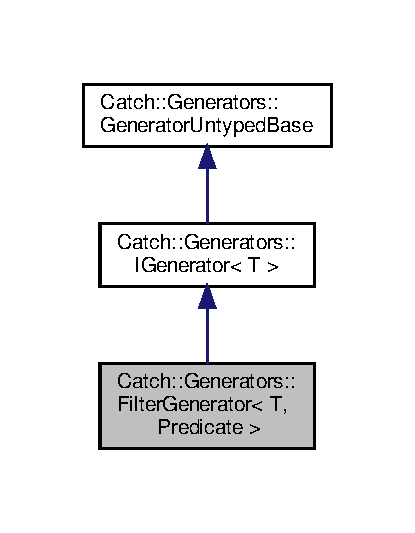
\includegraphics[width=199pt]{classCatch_1_1Generators_1_1FilterGenerator__inherit__graph}
\end{center}
\end{figure}


Collaboration diagram for Catch\+:\+:Generators\+:\+:Filter\+Generator$<$ T, Predicate $>$\+:
\nopagebreak
\begin{figure}[H]
\begin{center}
\leavevmode
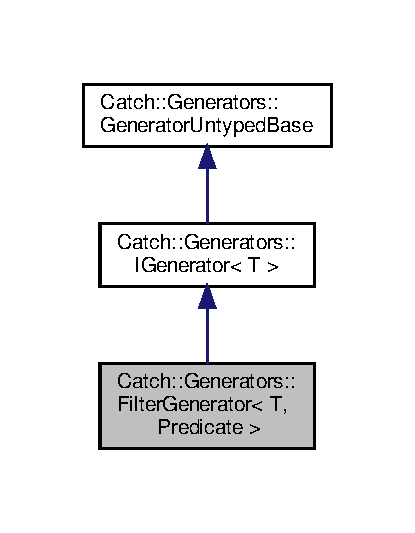
\includegraphics[width=199pt]{classCatch_1_1Generators_1_1FilterGenerator__coll__graph}
\end{center}
\end{figure}
\subsection*{Public Member Functions}
\begin{DoxyCompactItemize}
\item 
\mbox{\Hypertarget{classCatch_1_1Generators_1_1FilterGenerator_aa16886a5e41cbd3b6ffa3dd52388a3a1}\label{classCatch_1_1Generators_1_1FilterGenerator_aa16886a5e41cbd3b6ffa3dd52388a3a1}} 
{\footnotesize template$<$typename P  = Predicate$>$ }\\{\bfseries Filter\+Generator} (P \&\&pred, \hyperlink{classCatch_1_1Generators_1_1GeneratorWrapper}{Generator\+Wrapper}$<$ T $>$ \&\&generator)
\item 
\mbox{\Hypertarget{classCatch_1_1Generators_1_1FilterGenerator_ab30e81b61a77430661d40f814758f6fe}\label{classCatch_1_1Generators_1_1FilterGenerator_ab30e81b61a77430661d40f814758f6fe}} 
T const  \& {\bfseries get} () const override
\item 
\mbox{\Hypertarget{classCatch_1_1Generators_1_1FilterGenerator_a02ce0839dcaa7545c55d0fe70cc50e84}\label{classCatch_1_1Generators_1_1FilterGenerator_a02ce0839dcaa7545c55d0fe70cc50e84}} 
bool {\bfseries next} () override
\end{DoxyCompactItemize}
\subsection*{Private Attributes}
\begin{DoxyCompactItemize}
\item 
\mbox{\Hypertarget{classCatch_1_1Generators_1_1FilterGenerator_a6fb6975b1401cf7bd7e76e3a542a45cf}\label{classCatch_1_1Generators_1_1FilterGenerator_a6fb6975b1401cf7bd7e76e3a542a45cf}} 
\hyperlink{classCatch_1_1Generators_1_1GeneratorWrapper}{Generator\+Wrapper}$<$ T $>$ {\bfseries m\+\_\+generator}
\item 
\mbox{\Hypertarget{classCatch_1_1Generators_1_1FilterGenerator_a51cda8aafad62eba1d26618f3ca8cff1}\label{classCatch_1_1Generators_1_1FilterGenerator_a51cda8aafad62eba1d26618f3ca8cff1}} 
Predicate {\bfseries m\+\_\+predicate}
\end{DoxyCompactItemize}
\subsection*{Additional Inherited Members}


The documentation for this class was generated from the following file\+:\begin{DoxyCompactItemize}
\item 
/home/sinflair/\+P/crypto/\+A\+K/src/\+Praktikum-\/\+D\+E\+S/catch.\+hpp\end{DoxyCompactItemize}

\hypertarget{classCatch_1_1Generators_1_1FixedValuesGenerator}{}\section{Catch\+:\+:Generators\+:\+:Fixed\+Values\+Generator$<$ T $>$ Class Template Reference}
\label{classCatch_1_1Generators_1_1FixedValuesGenerator}\index{Catch\+::\+Generators\+::\+Fixed\+Values\+Generator$<$ T $>$@{Catch\+::\+Generators\+::\+Fixed\+Values\+Generator$<$ T $>$}}


Inheritance diagram for Catch\+:\+:Generators\+:\+:Fixed\+Values\+Generator$<$ T $>$\+:
\nopagebreak
\begin{figure}[H]
\begin{center}
\leavevmode
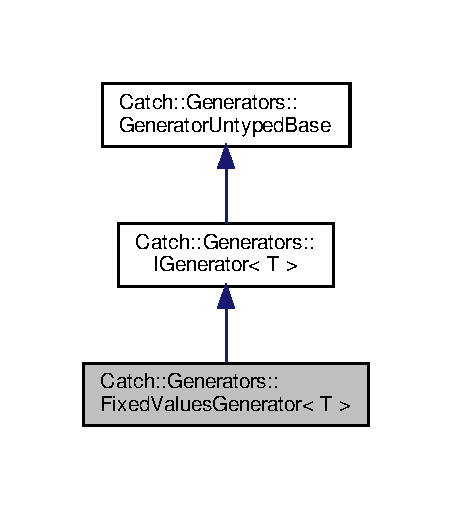
\includegraphics[width=217pt]{classCatch_1_1Generators_1_1FixedValuesGenerator__inherit__graph}
\end{center}
\end{figure}


Collaboration diagram for Catch\+:\+:Generators\+:\+:Fixed\+Values\+Generator$<$ T $>$\+:
\nopagebreak
\begin{figure}[H]
\begin{center}
\leavevmode
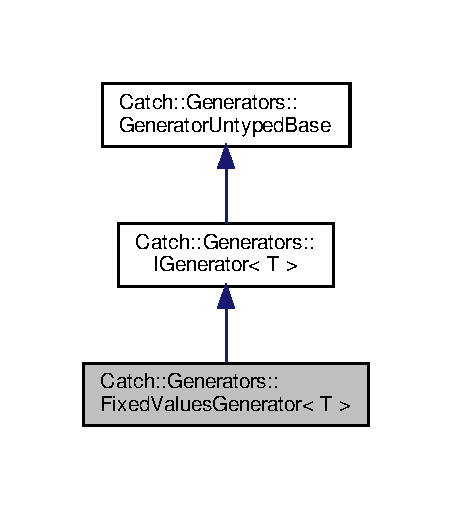
\includegraphics[width=217pt]{classCatch_1_1Generators_1_1FixedValuesGenerator__coll__graph}
\end{center}
\end{figure}
\subsection*{Public Member Functions}
\begin{DoxyCompactItemize}
\item 
\mbox{\Hypertarget{classCatch_1_1Generators_1_1FixedValuesGenerator_a6e9f473655413c1cb15f079890f06b86}\label{classCatch_1_1Generators_1_1FixedValuesGenerator_a6e9f473655413c1cb15f079890f06b86}} 
{\bfseries Fixed\+Values\+Generator} (std\+::initializer\+\_\+list$<$ T $>$ values)
\item 
\mbox{\Hypertarget{classCatch_1_1Generators_1_1FixedValuesGenerator_ad2ea8c959c600386bcc4b2656b40d33e}\label{classCatch_1_1Generators_1_1FixedValuesGenerator_ad2ea8c959c600386bcc4b2656b40d33e}} 
T const  \& {\bfseries get} () const override
\item 
\mbox{\Hypertarget{classCatch_1_1Generators_1_1FixedValuesGenerator_a6ce9e3ed045239c7b82873f24bd9cd3b}\label{classCatch_1_1Generators_1_1FixedValuesGenerator_a6ce9e3ed045239c7b82873f24bd9cd3b}} 
bool {\bfseries next} () override
\end{DoxyCompactItemize}
\subsection*{Private Attributes}
\begin{DoxyCompactItemize}
\item 
\mbox{\Hypertarget{classCatch_1_1Generators_1_1FixedValuesGenerator_a591837f944b435858bc3b9fa73502ee6}\label{classCatch_1_1Generators_1_1FixedValuesGenerator_a591837f944b435858bc3b9fa73502ee6}} 
std\+::vector$<$ T $>$ {\bfseries m\+\_\+values}
\item 
\mbox{\Hypertarget{classCatch_1_1Generators_1_1FixedValuesGenerator_a14c3c77deb624c09065e5ccaf8646f33}\label{classCatch_1_1Generators_1_1FixedValuesGenerator_a14c3c77deb624c09065e5ccaf8646f33}} 
size\+\_\+t {\bfseries m\+\_\+idx} = 0
\end{DoxyCompactItemize}
\subsection*{Additional Inherited Members}


The documentation for this class was generated from the following file\+:\begin{DoxyCompactItemize}
\item 
/home/sinflair/\+P/crypto/\+A\+K/src/\+Praktikum-\/\+D\+E\+S/catch.\+hpp\end{DoxyCompactItemize}

\hypertarget{classCatch_1_1GeneratorException}{}\section{Catch\+:\+:Generator\+Exception Class Reference}
\label{classCatch_1_1GeneratorException}\index{Catch\+::\+Generator\+Exception@{Catch\+::\+Generator\+Exception}}


Inheritance diagram for Catch\+:\+:Generator\+Exception\+:
\nopagebreak
\begin{figure}[H]
\begin{center}
\leavevmode
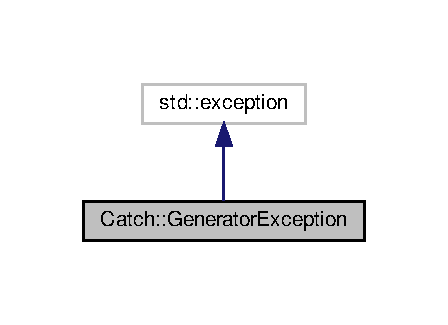
\includegraphics[width=215pt]{classCatch_1_1GeneratorException__inherit__graph}
\end{center}
\end{figure}


Collaboration diagram for Catch\+:\+:Generator\+Exception\+:
\nopagebreak
\begin{figure}[H]
\begin{center}
\leavevmode
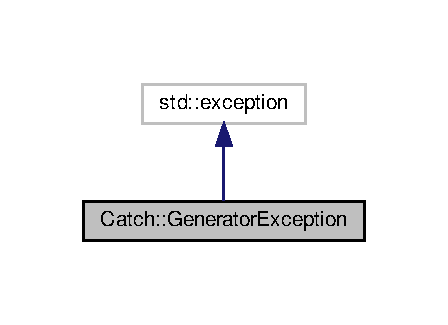
\includegraphics[width=215pt]{classCatch_1_1GeneratorException__coll__graph}
\end{center}
\end{figure}
\subsection*{Public Member Functions}
\begin{DoxyCompactItemize}
\item 
\mbox{\Hypertarget{classCatch_1_1GeneratorException_a3cf9282d555ec32389665ce723bf36ea}\label{classCatch_1_1GeneratorException_a3cf9282d555ec32389665ce723bf36ea}} 
{\bfseries Generator\+Exception} (const char $\ast$msg)
\item 
\mbox{\Hypertarget{classCatch_1_1GeneratorException_ade029163144d136f12187e5b9a0161d5}\label{classCatch_1_1GeneratorException_ade029163144d136f12187e5b9a0161d5}} 
const char $\ast$ {\bfseries what} () const noexcept override final
\end{DoxyCompactItemize}
\subsection*{Private Attributes}
\begin{DoxyCompactItemize}
\item 
\mbox{\Hypertarget{classCatch_1_1GeneratorException_a493b6ec9e3be0e3852de73c87dba6e5e}\label{classCatch_1_1GeneratorException_a493b6ec9e3be0e3852de73c87dba6e5e}} 
const char $\ast$const {\bfseries m\+\_\+msg} = \char`\"{}\char`\"{}
\end{DoxyCompactItemize}


The documentation for this class was generated from the following file\+:\begin{DoxyCompactItemize}
\item 
/home/sinflair/\+P/crypto/\+A\+K/src/\+Praktikum-\/\+D\+E\+S/catch.\+hpp\end{DoxyCompactItemize}

\hypertarget{classCatch_1_1Generators_1_1Generators}{}\section{Catch\+:\+:Generators\+:\+:Generators$<$ T $>$ Class Template Reference}
\label{classCatch_1_1Generators_1_1Generators}\index{Catch\+::\+Generators\+::\+Generators$<$ T $>$@{Catch\+::\+Generators\+::\+Generators$<$ T $>$}}


Inheritance diagram for Catch\+:\+:Generators\+:\+:Generators$<$ T $>$\+:
\nopagebreak
\begin{figure}[H]
\begin{center}
\leavevmode
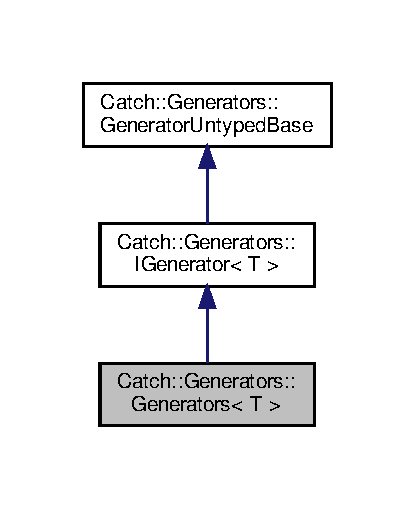
\includegraphics[width=199pt]{classCatch_1_1Generators_1_1Generators__inherit__graph}
\end{center}
\end{figure}


Collaboration diagram for Catch\+:\+:Generators\+:\+:Generators$<$ T $>$\+:
\nopagebreak
\begin{figure}[H]
\begin{center}
\leavevmode
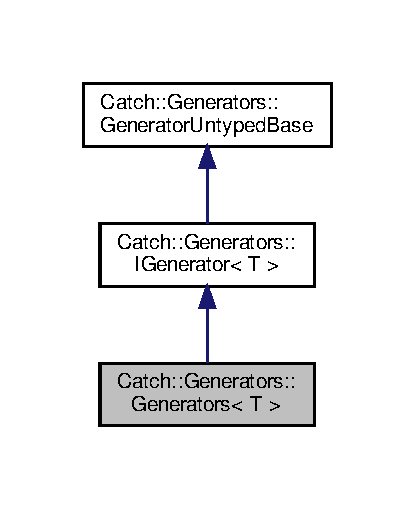
\includegraphics[width=199pt]{classCatch_1_1Generators_1_1Generators__coll__graph}
\end{center}
\end{figure}
\subsection*{Public Member Functions}
\begin{DoxyCompactItemize}
\item 
\mbox{\Hypertarget{classCatch_1_1Generators_1_1Generators_a0288170b30cd0fdfef6efc2d9bc8acba}\label{classCatch_1_1Generators_1_1Generators_a0288170b30cd0fdfef6efc2d9bc8acba}} 
{\footnotesize template$<$typename... Gs$>$ }\\{\bfseries Generators} (Gs... more\+Generators)
\item 
\mbox{\Hypertarget{classCatch_1_1Generators_1_1Generators_a66705482b7efa88cae6e6b7062d5de6a}\label{classCatch_1_1Generators_1_1Generators_a66705482b7efa88cae6e6b7062d5de6a}} 
T const  \& {\bfseries get} () const override
\item 
\mbox{\Hypertarget{classCatch_1_1Generators_1_1Generators_ad127fd2a07347b527f79ab3b78bd40fb}\label{classCatch_1_1Generators_1_1Generators_ad127fd2a07347b527f79ab3b78bd40fb}} 
bool {\bfseries next} () override
\end{DoxyCompactItemize}
\subsection*{Private Member Functions}
\begin{DoxyCompactItemize}
\item 
\mbox{\Hypertarget{classCatch_1_1Generators_1_1Generators_a56e1b82d4c9c952076cd58efbf7a4572}\label{classCatch_1_1Generators_1_1Generators_a56e1b82d4c9c952076cd58efbf7a4572}} 
void {\bfseries populate} (\hyperlink{classCatch_1_1Generators_1_1GeneratorWrapper}{Generator\+Wrapper}$<$ T $>$ \&\&generator)
\item 
\mbox{\Hypertarget{classCatch_1_1Generators_1_1Generators_ad708036fa5a9bf0cd1520ce111bc851d}\label{classCatch_1_1Generators_1_1Generators_ad708036fa5a9bf0cd1520ce111bc851d}} 
void {\bfseries populate} (T \&\&val)
\item 
\mbox{\Hypertarget{classCatch_1_1Generators_1_1Generators_a8ff8b7dda734d1808b644fefc67f4c98}\label{classCatch_1_1Generators_1_1Generators_a8ff8b7dda734d1808b644fefc67f4c98}} 
{\footnotesize template$<$typename U $>$ }\\void {\bfseries populate} (U \&\&val)
\item 
\mbox{\Hypertarget{classCatch_1_1Generators_1_1Generators_a4b9680ee28e48e4dc4c4538b5510e649}\label{classCatch_1_1Generators_1_1Generators_a4b9680ee28e48e4dc4c4538b5510e649}} 
{\footnotesize template$<$typename U , typename... Gs$>$ }\\void {\bfseries populate} (U \&\&value\+Or\+Generator, Gs... more\+Generators)
\end{DoxyCompactItemize}
\subsection*{Private Attributes}
\begin{DoxyCompactItemize}
\item 
\mbox{\Hypertarget{classCatch_1_1Generators_1_1Generators_a4d41bb9f0e8d726a8a53c86354bf19de}\label{classCatch_1_1Generators_1_1Generators_a4d41bb9f0e8d726a8a53c86354bf19de}} 
std\+::vector$<$ \hyperlink{classCatch_1_1Generators_1_1GeneratorWrapper}{Generator\+Wrapper}$<$ T $>$ $>$ {\bfseries m\+\_\+generators}
\item 
\mbox{\Hypertarget{classCatch_1_1Generators_1_1Generators_a8f5cd6b2479cfadbd45033c4ad17ff0c}\label{classCatch_1_1Generators_1_1Generators_a8f5cd6b2479cfadbd45033c4ad17ff0c}} 
size\+\_\+t {\bfseries m\+\_\+current} = 0
\end{DoxyCompactItemize}
\subsection*{Additional Inherited Members}


The documentation for this class was generated from the following file\+:\begin{DoxyCompactItemize}
\item 
/home/sinflair/\+P/crypto/\+A\+K/src/\+Praktikum-\/\+D\+E\+S/catch.\+hpp\end{DoxyCompactItemize}

\hypertarget{classCatch_1_1Generators_1_1GeneratorUntypedBase}{}\section{Catch\+:\+:Generators\+:\+:Generator\+Untyped\+Base Class Reference}
\label{classCatch_1_1Generators_1_1GeneratorUntypedBase}\index{Catch\+::\+Generators\+::\+Generator\+Untyped\+Base@{Catch\+::\+Generators\+::\+Generator\+Untyped\+Base}}


Inheritance diagram for Catch\+:\+:Generators\+:\+:Generator\+Untyped\+Base\+:
\nopagebreak
\begin{figure}[H]
\begin{center}
\leavevmode
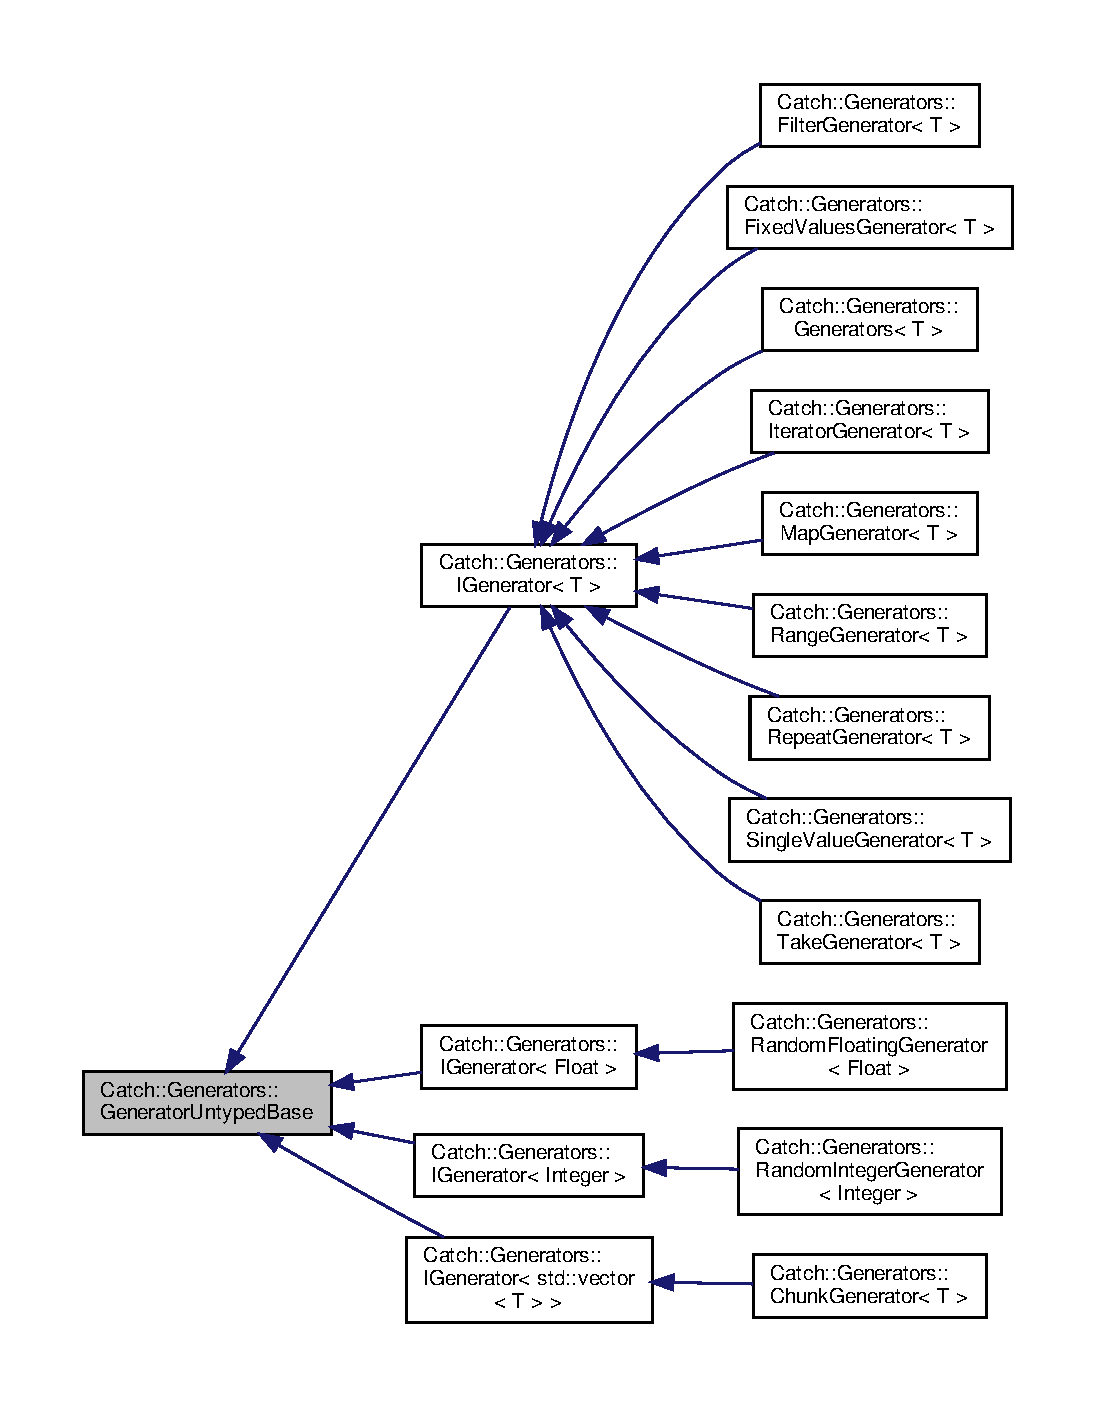
\includegraphics[width=350pt]{classCatch_1_1Generators_1_1GeneratorUntypedBase__inherit__graph}
\end{center}
\end{figure}
\subsection*{Public Member Functions}
\begin{DoxyCompactItemize}
\item 
\mbox{\Hypertarget{classCatch_1_1Generators_1_1GeneratorUntypedBase_aeed3c0cd6233c5f553549e453b8d6638}\label{classCatch_1_1Generators_1_1GeneratorUntypedBase_aeed3c0cd6233c5f553549e453b8d6638}} 
virtual bool {\bfseries next} ()=0
\end{DoxyCompactItemize}


The documentation for this class was generated from the following file\+:\begin{DoxyCompactItemize}
\item 
/home/sinflair/\+P/crypto/\+A\+K/src/\+Praktikum-\/\+D\+E\+S/catch.\+hpp\end{DoxyCompactItemize}

\hypertarget{classCatch_1_1Generators_1_1GeneratorWrapper}{}\section{Catch\+:\+:Generators\+:\+:Generator\+Wrapper$<$ T $>$ Class Template Reference}
\label{classCatch_1_1Generators_1_1GeneratorWrapper}\index{Catch\+::\+Generators\+::\+Generator\+Wrapper$<$ T $>$@{Catch\+::\+Generators\+::\+Generator\+Wrapper$<$ T $>$}}
\subsection*{Public Member Functions}
\begin{DoxyCompactItemize}
\item 
\mbox{\Hypertarget{classCatch_1_1Generators_1_1GeneratorWrapper_aecffeafd4fd38d91a52dadf28b6e2b29}\label{classCatch_1_1Generators_1_1GeneratorWrapper_aecffeafd4fd38d91a52dadf28b6e2b29}} 
{\bfseries Generator\+Wrapper} (std\+::unique\+\_\+ptr$<$ \hyperlink{structCatch_1_1Generators_1_1IGenerator}{I\+Generator}$<$ T $>$$>$ generator)
\item 
\mbox{\Hypertarget{classCatch_1_1Generators_1_1GeneratorWrapper_a271f0f905f2c473c907550435b81e102}\label{classCatch_1_1Generators_1_1GeneratorWrapper_a271f0f905f2c473c907550435b81e102}} 
T const  \& {\bfseries get} () const
\item 
\mbox{\Hypertarget{classCatch_1_1Generators_1_1GeneratorWrapper_acbfdca94811ae02461bd2cf5f60b666e}\label{classCatch_1_1Generators_1_1GeneratorWrapper_acbfdca94811ae02461bd2cf5f60b666e}} 
bool {\bfseries next} ()
\end{DoxyCompactItemize}
\subsection*{Private Attributes}
\begin{DoxyCompactItemize}
\item 
\mbox{\Hypertarget{classCatch_1_1Generators_1_1GeneratorWrapper_a8f35291599183b36e4c5af78e17d3a8c}\label{classCatch_1_1Generators_1_1GeneratorWrapper_a8f35291599183b36e4c5af78e17d3a8c}} 
std\+::unique\+\_\+ptr$<$ \hyperlink{structCatch_1_1Generators_1_1IGenerator}{I\+Generator}$<$ T $>$ $>$ {\bfseries m\+\_\+generator}
\end{DoxyCompactItemize}


The documentation for this class was generated from the following file\+:\begin{DoxyCompactItemize}
\item 
/home/sinflair/\+P/crypto/\+A\+K/src/\+Praktikum-\/\+D\+E\+S/catch.\+hpp\end{DoxyCompactItemize}

\hypertarget{structgengetopt__args__info}{}\section{gengetopt\+\_\+args\+\_\+info Struct Reference}
\label{structgengetopt__args__info}\index{gengetopt\+\_\+args\+\_\+info@{gengetopt\+\_\+args\+\_\+info}}


Where the command line options are stored.  




{\ttfamily \#include $<$aes-\/getopt.\+h$>$}

\subsection*{Public Attributes}
\begin{DoxyCompactItemize}
\item 
\mbox{\Hypertarget{structgengetopt__args__info_afb4efa68a6f43a4d112e9b96ffe89101}\label{structgengetopt__args__info_afb4efa68a6f43a4d112e9b96ffe89101}} 
const char $\ast$ \hyperlink{structgengetopt__args__info_afb4efa68a6f43a4d112e9b96ffe89101}{help\+\_\+help}
\begin{DoxyCompactList}\small\item\em Print help and exit help description. \end{DoxyCompactList}\item 
\mbox{\Hypertarget{structgengetopt__args__info_adef454ea6f3ff4114ae5009e58360cfc}\label{structgengetopt__args__info_adef454ea6f3ff4114ae5009e58360cfc}} 
const char $\ast$ \hyperlink{structgengetopt__args__info_adef454ea6f3ff4114ae5009e58360cfc}{version\+\_\+help}
\begin{DoxyCompactList}\small\item\em Print version and exit help description. \end{DoxyCompactList}\item 
\mbox{\Hypertarget{structgengetopt__args__info_a9d2e2cfeae6c1b4644a9e539dd37b490}\label{structgengetopt__args__info_a9d2e2cfeae6c1b4644a9e539dd37b490}} 
char $\ast$ \hyperlink{structgengetopt__args__info_a9d2e2cfeae6c1b4644a9e539dd37b490}{key\+\_\+arg}
\begin{DoxyCompactList}\small\item\em Key to be used for encryption or decryption. \end{DoxyCompactList}\item 
\mbox{\Hypertarget{structgengetopt__args__info_a46fe55fd04263db7ebf4d5afa09f696f}\label{structgengetopt__args__info_a46fe55fd04263db7ebf4d5afa09f696f}} 
char $\ast$ \hyperlink{structgengetopt__args__info_a46fe55fd04263db7ebf4d5afa09f696f}{key\+\_\+orig}
\begin{DoxyCompactList}\small\item\em Key to be used for encryption or decryption original value given at command line. \end{DoxyCompactList}\item 
\mbox{\Hypertarget{structgengetopt__args__info_a9f98c455fbbd65117dbbd1e17723c92e}\label{structgengetopt__args__info_a9f98c455fbbd65117dbbd1e17723c92e}} 
const char $\ast$ \hyperlink{structgengetopt__args__info_a9f98c455fbbd65117dbbd1e17723c92e}{key\+\_\+help}
\begin{DoxyCompactList}\small\item\em Key to be used for encryption or decryption help description. \end{DoxyCompactList}\item 
\mbox{\Hypertarget{structgengetopt__args__info_a1022ab6bd8cfa9596789a6a7059be6af}\label{structgengetopt__args__info_a1022ab6bd8cfa9596789a6a7059be6af}} 
char $\ast$ \hyperlink{structgengetopt__args__info_a1022ab6bd8cfa9596789a6a7059be6af}{out\+\_\+arg}
\begin{DoxyCompactList}\small\item\em output file. \end{DoxyCompactList}\item 
\mbox{\Hypertarget{structgengetopt__args__info_a342bcb7cbcac1cbaefd3ffaafa3736ff}\label{structgengetopt__args__info_a342bcb7cbcac1cbaefd3ffaafa3736ff}} 
char $\ast$ \hyperlink{structgengetopt__args__info_a342bcb7cbcac1cbaefd3ffaafa3736ff}{out\+\_\+orig}
\begin{DoxyCompactList}\small\item\em output file original value given at command line. \end{DoxyCompactList}\item 
\mbox{\Hypertarget{structgengetopt__args__info_ad1e0068ecb61c96fc1b239c575d125d9}\label{structgengetopt__args__info_ad1e0068ecb61c96fc1b239c575d125d9}} 
const char $\ast$ \hyperlink{structgengetopt__args__info_ad1e0068ecb61c96fc1b239c575d125d9}{out\+\_\+help}
\begin{DoxyCompactList}\small\item\em output file help description. \end{DoxyCompactList}\item 
\mbox{\Hypertarget{structgengetopt__args__info_a31a0c7c5b907732c8f4f74717bfdb8bc}\label{structgengetopt__args__info_a31a0c7c5b907732c8f4f74717bfdb8bc}} 
const char $\ast$ \hyperlink{structgengetopt__args__info_a31a0c7c5b907732c8f4f74717bfdb8bc}{encrypt\+\_\+help}
\begin{DoxyCompactList}\small\item\em Encryption help description. \end{DoxyCompactList}\item 
\mbox{\Hypertarget{structgengetopt__args__info_a1e9e71d6f662ce2a1eef16dd13f18ef4}\label{structgengetopt__args__info_a1e9e71d6f662ce2a1eef16dd13f18ef4}} 
const char $\ast$ \hyperlink{structgengetopt__args__info_a1e9e71d6f662ce2a1eef16dd13f18ef4}{decrypt\+\_\+help}
\begin{DoxyCompactList}\small\item\em Decryption help description. \end{DoxyCompactList}\item 
\mbox{\Hypertarget{structgengetopt__args__info_ab9fd677f890731fd7d6f6c62e6dfc99c}\label{structgengetopt__args__info_ab9fd677f890731fd7d6f6c62e6dfc99c}} 
unsigned int \hyperlink{structgengetopt__args__info_ab9fd677f890731fd7d6f6c62e6dfc99c}{help\+\_\+given}
\begin{DoxyCompactList}\small\item\em Whether help was given. \end{DoxyCompactList}\item 
\mbox{\Hypertarget{structgengetopt__args__info_ad4953a2130b2f8b94a3a687014f278e1}\label{structgengetopt__args__info_ad4953a2130b2f8b94a3a687014f278e1}} 
unsigned int \hyperlink{structgengetopt__args__info_ad4953a2130b2f8b94a3a687014f278e1}{version\+\_\+given}
\begin{DoxyCompactList}\small\item\em Whether version was given. \end{DoxyCompactList}\item 
\mbox{\Hypertarget{structgengetopt__args__info_a155a1a709ea64f935a0cda6ebe932f33}\label{structgengetopt__args__info_a155a1a709ea64f935a0cda6ebe932f33}} 
unsigned int \hyperlink{structgengetopt__args__info_a155a1a709ea64f935a0cda6ebe932f33}{key\+\_\+given}
\begin{DoxyCompactList}\small\item\em Whether key was given. \end{DoxyCompactList}\item 
\mbox{\Hypertarget{structgengetopt__args__info_a0b95b56ea8bfba9d7d1dfc92a1ba8feb}\label{structgengetopt__args__info_a0b95b56ea8bfba9d7d1dfc92a1ba8feb}} 
unsigned int \hyperlink{structgengetopt__args__info_a0b95b56ea8bfba9d7d1dfc92a1ba8feb}{out\+\_\+given}
\begin{DoxyCompactList}\small\item\em Whether out was given. \end{DoxyCompactList}\item 
\mbox{\Hypertarget{structgengetopt__args__info_a2cc94a70a7e771ee78c947d08dd8cf1d}\label{structgengetopt__args__info_a2cc94a70a7e771ee78c947d08dd8cf1d}} 
unsigned int \hyperlink{structgengetopt__args__info_a2cc94a70a7e771ee78c947d08dd8cf1d}{encrypt\+\_\+given}
\begin{DoxyCompactList}\small\item\em Whether encrypt was given. \end{DoxyCompactList}\item 
\mbox{\Hypertarget{structgengetopt__args__info_ab8fb4a2ce4915d98294802d3b361325f}\label{structgengetopt__args__info_ab8fb4a2ce4915d98294802d3b361325f}} 
unsigned int \hyperlink{structgengetopt__args__info_ab8fb4a2ce4915d98294802d3b361325f}{decrypt\+\_\+given}
\begin{DoxyCompactList}\small\item\em Whether decrypt was given. \end{DoxyCompactList}\item 
\mbox{\Hypertarget{structgengetopt__args__info_a9604690019dd09b318302dae6868726c}\label{structgengetopt__args__info_a9604690019dd09b318302dae6868726c}} 
char $\ast$$\ast$ \hyperlink{structgengetopt__args__info_a9604690019dd09b318302dae6868726c}{inputs}
\begin{DoxyCompactList}\small\item\em unamed options (options without names) \end{DoxyCompactList}\item 
\mbox{\Hypertarget{structgengetopt__args__info_a3d69c180d5ac0b1124fd9a6fe680706c}\label{structgengetopt__args__info_a3d69c180d5ac0b1124fd9a6fe680706c}} 
unsigned \hyperlink{structgengetopt__args__info_a3d69c180d5ac0b1124fd9a6fe680706c}{inputs\+\_\+num}
\begin{DoxyCompactList}\small\item\em unamed options number \end{DoxyCompactList}\item 
\mbox{\Hypertarget{structgengetopt__args__info_a44f277219c706b8ca8b64ce3d9f3f2ec}\label{structgengetopt__args__info_a44f277219c706b8ca8b64ce3d9f3f2ec}} 
int \hyperlink{structgengetopt__args__info_a44f277219c706b8ca8b64ce3d9f3f2ec}{opmode\+\_\+group\+\_\+counter}
\begin{DoxyCompactList}\small\item\em Counter for group opmode. \end{DoxyCompactList}\end{DoxyCompactItemize}


\subsection{Detailed Description}
Where the command line options are stored. 

The documentation for this struct was generated from the following file\+:\begin{DoxyCompactItemize}
\item 
/home/sinflair/\+P/crypto/\+A\+K/src/\+Praktikum-\/\+A\+E\+S/\hyperlink{aes-getopt_8h}{aes-\/getopt.\+h}\end{DoxyCompactItemize}

\hypertarget{structCatch_1_1IConfig}{}\section{Catch\+:\+:I\+Config Struct Reference}
\label{structCatch_1_1IConfig}\index{Catch\+::\+I\+Config@{Catch\+::\+I\+Config}}


Inheritance diagram for Catch\+:\+:I\+Config\+:
\nopagebreak
\begin{figure}[H]
\begin{center}
\leavevmode
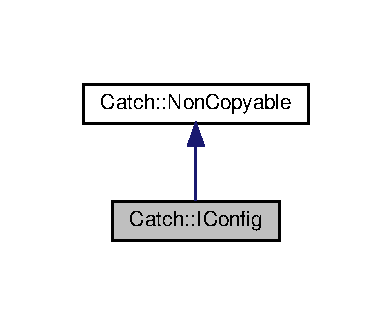
\includegraphics[width=188pt]{structCatch_1_1IConfig__inherit__graph}
\end{center}
\end{figure}


Collaboration diagram for Catch\+:\+:I\+Config\+:
\nopagebreak
\begin{figure}[H]
\begin{center}
\leavevmode
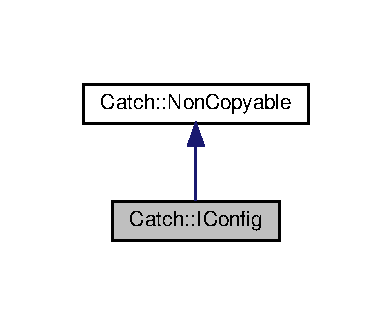
\includegraphics[width=188pt]{structCatch_1_1IConfig__coll__graph}
\end{center}
\end{figure}
\subsection*{Public Member Functions}
\begin{DoxyCompactItemize}
\item 
\mbox{\Hypertarget{structCatch_1_1IConfig_aadb95f849359de1e6eb915aab063e542}\label{structCatch_1_1IConfig_aadb95f849359de1e6eb915aab063e542}} 
virtual bool {\bfseries allow\+Throws} () const =0
\item 
\mbox{\Hypertarget{structCatch_1_1IConfig_aa4c3fe0825e7e6ebdcfa6abc7abf3617}\label{structCatch_1_1IConfig_aa4c3fe0825e7e6ebdcfa6abc7abf3617}} 
virtual std\+::ostream \& {\bfseries stream} () const =0
\item 
\mbox{\Hypertarget{structCatch_1_1IConfig_aa2315800a05c19db71518b1edc39d43b}\label{structCatch_1_1IConfig_aa2315800a05c19db71518b1edc39d43b}} 
virtual std\+::string {\bfseries name} () const =0
\item 
\mbox{\Hypertarget{structCatch_1_1IConfig_a2f1b0391019b9ce69921527a684eab23}\label{structCatch_1_1IConfig_a2f1b0391019b9ce69921527a684eab23}} 
virtual bool {\bfseries include\+Successful\+Results} () const =0
\item 
\mbox{\Hypertarget{structCatch_1_1IConfig_a5b886c5aad9001e90f63a7cf0726af63}\label{structCatch_1_1IConfig_a5b886c5aad9001e90f63a7cf0726af63}} 
virtual bool {\bfseries should\+Debug\+Break} () const =0
\item 
\mbox{\Hypertarget{structCatch_1_1IConfig_a75d970c495a28e46b8e9b04a1d32149f}\label{structCatch_1_1IConfig_a75d970c495a28e46b8e9b04a1d32149f}} 
virtual bool {\bfseries warn\+About\+Missing\+Assertions} () const =0
\item 
\mbox{\Hypertarget{structCatch_1_1IConfig_a30590623e3918825f2896c2262bf6fe3}\label{structCatch_1_1IConfig_a30590623e3918825f2896c2262bf6fe3}} 
virtual bool {\bfseries warn\+About\+No\+Tests} () const =0
\item 
\mbox{\Hypertarget{structCatch_1_1IConfig_a363f3388a439d02217f37198eff96744}\label{structCatch_1_1IConfig_a363f3388a439d02217f37198eff96744}} 
virtual int {\bfseries abort\+After} () const =0
\item 
\mbox{\Hypertarget{structCatch_1_1IConfig_aa288bf92ccd0aafd85409d8aefdf738c}\label{structCatch_1_1IConfig_aa288bf92ccd0aafd85409d8aefdf738c}} 
virtual bool {\bfseries show\+Invisibles} () const =0
\item 
\mbox{\Hypertarget{structCatch_1_1IConfig_abaa97d281484278291f0d3db6d404aeb}\label{structCatch_1_1IConfig_abaa97d281484278291f0d3db6d404aeb}} 
virtual Show\+Durations\+::\+Or\+Not {\bfseries show\+Durations} () const =0
\item 
\mbox{\Hypertarget{structCatch_1_1IConfig_a03a2fd8221d896d12bf3684ab2a03588}\label{structCatch_1_1IConfig_a03a2fd8221d896d12bf3684ab2a03588}} 
virtual Test\+Spec const  \& {\bfseries test\+Spec} () const =0
\item 
\mbox{\Hypertarget{structCatch_1_1IConfig_a49a475bbeb3180c06799d6d958914649}\label{structCatch_1_1IConfig_a49a475bbeb3180c06799d6d958914649}} 
virtual bool {\bfseries has\+Test\+Filters} () const =0
\item 
\mbox{\Hypertarget{structCatch_1_1IConfig_a1b8a299344a493eb98c12faae48421d7}\label{structCatch_1_1IConfig_a1b8a299344a493eb98c12faae48421d7}} 
virtual std\+::vector$<$ std\+::string $>$ const  \& {\bfseries get\+Tests\+Or\+Tags} () const =0
\item 
\mbox{\Hypertarget{structCatch_1_1IConfig_a0fc59c9aba1d4018538d5526daa5eb78}\label{structCatch_1_1IConfig_a0fc59c9aba1d4018538d5526daa5eb78}} 
virtual Run\+Tests\+::\+In\+What\+Order {\bfseries run\+Order} () const =0
\item 
\mbox{\Hypertarget{structCatch_1_1IConfig_ae049eb45979d841073fa65d1094c7f14}\label{structCatch_1_1IConfig_ae049eb45979d841073fa65d1094c7f14}} 
virtual unsigned int {\bfseries rng\+Seed} () const =0
\item 
\mbox{\Hypertarget{structCatch_1_1IConfig_a87ec19a6b486eb5b5015cf7738fee026}\label{structCatch_1_1IConfig_a87ec19a6b486eb5b5015cf7738fee026}} 
virtual Use\+Colour\+::\+Yes\+Or\+No {\bfseries use\+Colour} () const =0
\item 
\mbox{\Hypertarget{structCatch_1_1IConfig_afc801995e115557f90e41f3d6e96908d}\label{structCatch_1_1IConfig_afc801995e115557f90e41f3d6e96908d}} 
virtual std\+::vector$<$ std\+::string $>$ const  \& {\bfseries get\+Sections\+To\+Run} () const =0
\item 
\mbox{\Hypertarget{structCatch_1_1IConfig_a55aff5924bdbb3f558775821b1eb4b3d}\label{structCatch_1_1IConfig_a55aff5924bdbb3f558775821b1eb4b3d}} 
virtual Verbosity {\bfseries verbosity} () const =0
\item 
\mbox{\Hypertarget{structCatch_1_1IConfig_aa9aa1eafdbe510e27bf319233969ee2c}\label{structCatch_1_1IConfig_aa9aa1eafdbe510e27bf319233969ee2c}} 
virtual bool {\bfseries benchmark\+No\+Analysis} () const =0
\item 
\mbox{\Hypertarget{structCatch_1_1IConfig_a583734a61796b495b80779a6540eb6cc}\label{structCatch_1_1IConfig_a583734a61796b495b80779a6540eb6cc}} 
virtual int {\bfseries benchmark\+Samples} () const =0
\item 
\mbox{\Hypertarget{structCatch_1_1IConfig_ae1ec73d460a2b58c7c9b022a430a34dd}\label{structCatch_1_1IConfig_ae1ec73d460a2b58c7c9b022a430a34dd}} 
virtual double {\bfseries benchmark\+Confidence\+Interval} () const =0
\item 
\mbox{\Hypertarget{structCatch_1_1IConfig_a3b8e5581be01f4773593f8b85eb7db98}\label{structCatch_1_1IConfig_a3b8e5581be01f4773593f8b85eb7db98}} 
virtual unsigned int {\bfseries benchmark\+Resamples} () const =0
\end{DoxyCompactItemize}


The documentation for this struct was generated from the following file\+:\begin{DoxyCompactItemize}
\item 
/home/sinflair/\+P/crypto/\+A\+K/src/\+Praktikum-\/\+D\+E\+S/catch.\+hpp\end{DoxyCompactItemize}

\hypertarget{structCatch_1_1IContext}{}\section{Catch\+:\+:I\+Context Struct Reference}
\label{structCatch_1_1IContext}\index{Catch\+::\+I\+Context@{Catch\+::\+I\+Context}}


Inheritance diagram for Catch\+:\+:I\+Context\+:
\nopagebreak
\begin{figure}[H]
\begin{center}
\leavevmode
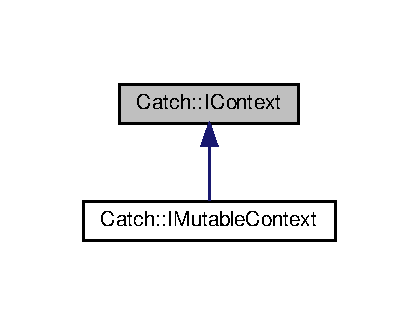
\includegraphics[width=201pt]{structCatch_1_1IContext__inherit__graph}
\end{center}
\end{figure}
\subsection*{Public Member Functions}
\begin{DoxyCompactItemize}
\item 
\mbox{\Hypertarget{structCatch_1_1IContext_a684e4ae71d1fdf3060c352ecde1d122f}\label{structCatch_1_1IContext_a684e4ae71d1fdf3060c352ecde1d122f}} 
virtual \hyperlink{structCatch_1_1IResultCapture}{I\+Result\+Capture} $\ast$ {\bfseries get\+Result\+Capture} ()=0
\item 
\mbox{\Hypertarget{structCatch_1_1IContext_af088415dde18d039ed5a2f95b02767c6}\label{structCatch_1_1IContext_af088415dde18d039ed5a2f95b02767c6}} 
virtual \hyperlink{structCatch_1_1IRunner}{I\+Runner} $\ast$ {\bfseries get\+Runner} ()=0
\item 
\mbox{\Hypertarget{structCatch_1_1IContext_a72a2718232adea8925fec9e71d3efd75}\label{structCatch_1_1IContext_a72a2718232adea8925fec9e71d3efd75}} 
virtual I\+Config\+Ptr const  \& {\bfseries get\+Config} () const =0
\end{DoxyCompactItemize}


The documentation for this struct was generated from the following file\+:\begin{DoxyCompactItemize}
\item 
/home/sinflair/\+P/crypto/\+A\+K/src/\+Praktikum-\/\+D\+E\+S/catch.\+hpp\end{DoxyCompactItemize}

\hypertarget{structCatch_1_1IExceptionTranslator}{}\section{Catch\+:\+:I\+Exception\+Translator Struct Reference}
\label{structCatch_1_1IExceptionTranslator}\index{Catch\+::\+I\+Exception\+Translator@{Catch\+::\+I\+Exception\+Translator}}


Inheritance diagram for Catch\+:\+:I\+Exception\+Translator\+:
\nopagebreak
\begin{figure}[H]
\begin{center}
\leavevmode
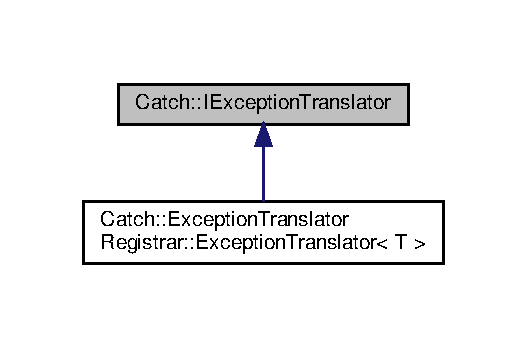
\includegraphics[width=253pt]{structCatch_1_1IExceptionTranslator__inherit__graph}
\end{center}
\end{figure}
\subsection*{Public Member Functions}
\begin{DoxyCompactItemize}
\item 
\mbox{\Hypertarget{structCatch_1_1IExceptionTranslator_a2a554b96ed5ed411e7c796b6b42837a5}\label{structCatch_1_1IExceptionTranslator_a2a554b96ed5ed411e7c796b6b42837a5}} 
virtual std\+::string {\bfseries translate} (Exception\+Translators\+::const\+\_\+iterator it, Exception\+Translators\+::const\+\_\+iterator it\+End) const =0
\end{DoxyCompactItemize}


The documentation for this struct was generated from the following file\+:\begin{DoxyCompactItemize}
\item 
/home/sinflair/\+P/crypto/\+A\+K/src/\+Praktikum-\/\+D\+E\+S/catch.\+hpp\end{DoxyCompactItemize}

\hypertarget{structCatch_1_1IExceptionTranslatorRegistry}{}\section{Catch\+:\+:I\+Exception\+Translator\+Registry Struct Reference}
\label{structCatch_1_1IExceptionTranslatorRegistry}\index{Catch\+::\+I\+Exception\+Translator\+Registry@{Catch\+::\+I\+Exception\+Translator\+Registry}}
\subsection*{Public Member Functions}
\begin{DoxyCompactItemize}
\item 
\mbox{\Hypertarget{structCatch_1_1IExceptionTranslatorRegistry_af76ae8c331a17f2a94c9720bc0d686bb}\label{structCatch_1_1IExceptionTranslatorRegistry_af76ae8c331a17f2a94c9720bc0d686bb}} 
virtual std\+::string {\bfseries translate\+Active\+Exception} () const =0
\end{DoxyCompactItemize}


The documentation for this struct was generated from the following file\+:\begin{DoxyCompactItemize}
\item 
/home/sinflair/\+P/crypto/\+A\+K/src/\+Praktikum-\/\+D\+E\+S/catch.\+hpp\end{DoxyCompactItemize}

\hypertarget{structCatch_1_1Generators_1_1IGenerator}{}\section{Catch\+:\+:Generators\+:\+:I\+Generator$<$ T $>$ Struct Template Reference}
\label{structCatch_1_1Generators_1_1IGenerator}\index{Catch\+::\+Generators\+::\+I\+Generator$<$ T $>$@{Catch\+::\+Generators\+::\+I\+Generator$<$ T $>$}}


Inheritance diagram for Catch\+:\+:Generators\+:\+:I\+Generator$<$ T $>$\+:
\nopagebreak
\begin{figure}[H]
\begin{center}
\leavevmode
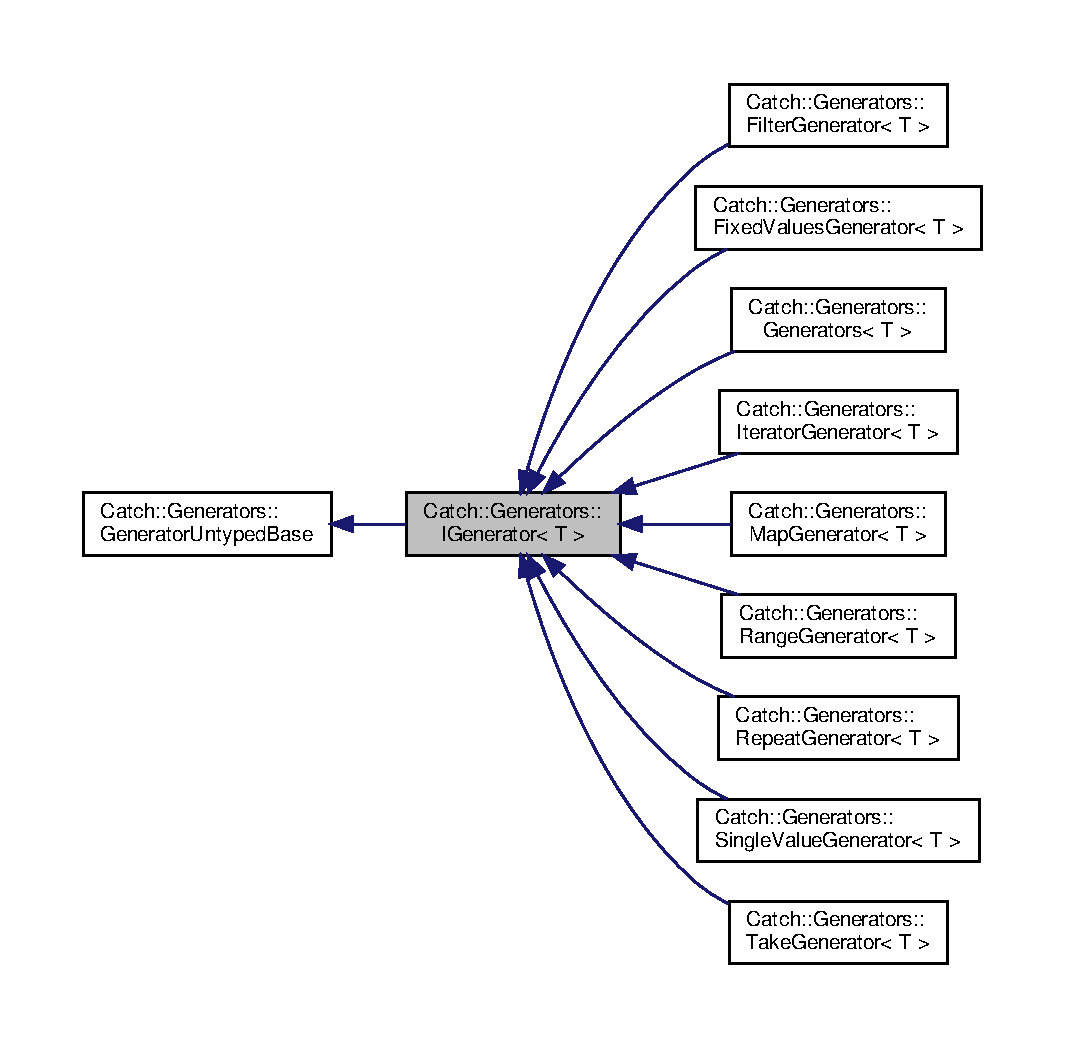
\includegraphics[width=350pt]{structCatch_1_1Generators_1_1IGenerator__inherit__graph}
\end{center}
\end{figure}


Collaboration diagram for Catch\+:\+:Generators\+:\+:I\+Generator$<$ T $>$\+:
\nopagebreak
\begin{figure}[H]
\begin{center}
\leavevmode
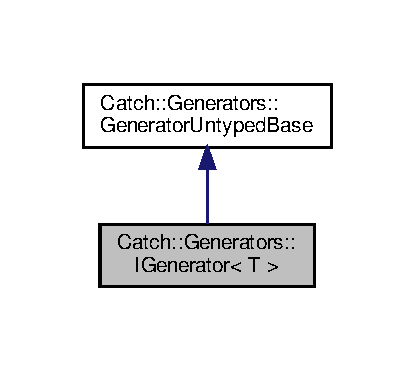
\includegraphics[width=199pt]{structCatch_1_1Generators_1_1IGenerator__coll__graph}
\end{center}
\end{figure}
\subsection*{Public Types}
\begin{DoxyCompactItemize}
\item 
\mbox{\Hypertarget{structCatch_1_1Generators_1_1IGenerator_a1f8677875fe0ff31f39c60d45504b9a5}\label{structCatch_1_1Generators_1_1IGenerator_a1f8677875fe0ff31f39c60d45504b9a5}} 
using {\bfseries type} = T
\end{DoxyCompactItemize}
\subsection*{Public Member Functions}
\begin{DoxyCompactItemize}
\item 
\mbox{\Hypertarget{structCatch_1_1Generators_1_1IGenerator_a525d381fc9249a885b075a0632a8579a}\label{structCatch_1_1Generators_1_1IGenerator_a525d381fc9249a885b075a0632a8579a}} 
virtual T const  \& {\bfseries get} () const =0
\end{DoxyCompactItemize}


The documentation for this struct was generated from the following file\+:\begin{DoxyCompactItemize}
\item 
/home/sinflair/\+P/crypto/\+A\+K/src/\+Praktikum-\/\+D\+E\+S/catch.\+hpp\end{DoxyCompactItemize}

\hypertarget{structCatch_1_1IGeneratorTracker}{}\section{Catch\+:\+:I\+Generator\+Tracker Struct Reference}
\label{structCatch_1_1IGeneratorTracker}\index{Catch\+::\+I\+Generator\+Tracker@{Catch\+::\+I\+Generator\+Tracker}}
\subsection*{Public Member Functions}
\begin{DoxyCompactItemize}
\item 
\mbox{\Hypertarget{structCatch_1_1IGeneratorTracker_ae88084f9af27c8b9a5d5775b9c148498}\label{structCatch_1_1IGeneratorTracker_ae88084f9af27c8b9a5d5775b9c148498}} 
virtual auto {\bfseries has\+Generator} () const -\/$>$ bool=0
\item 
\mbox{\Hypertarget{structCatch_1_1IGeneratorTracker_a23be942fc51672598bfa02c678c3078a}\label{structCatch_1_1IGeneratorTracker_a23be942fc51672598bfa02c678c3078a}} 
virtual auto {\bfseries get\+Generator} () const -\/$>$ Generators\+::\+Generator\+Base\+Ptr const \&=0
\item 
\mbox{\Hypertarget{structCatch_1_1IGeneratorTracker_a9945eff42219edc5a7071eebd8b0419e}\label{structCatch_1_1IGeneratorTracker_a9945eff42219edc5a7071eebd8b0419e}} 
virtual void {\bfseries set\+Generator} (Generators\+::\+Generator\+Base\+Ptr \&\&generator)=0
\end{DoxyCompactItemize}


The documentation for this struct was generated from the following file\+:\begin{DoxyCompactItemize}
\item 
/home/sinflair/\+P/crypto/\+A\+K/src/\+Praktikum-\/\+D\+E\+S/catch.\+hpp\end{DoxyCompactItemize}

\hypertarget{structCatch_1_1IMutableContext}{}\section{Catch\+:\+:I\+Mutable\+Context Struct Reference}
\label{structCatch_1_1IMutableContext}\index{Catch\+::\+I\+Mutable\+Context@{Catch\+::\+I\+Mutable\+Context}}


Inheritance diagram for Catch\+:\+:I\+Mutable\+Context\+:
\nopagebreak
\begin{figure}[H]
\begin{center}
\leavevmode
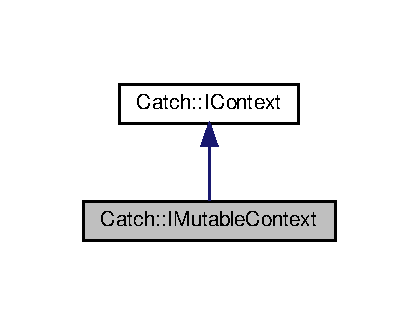
\includegraphics[width=201pt]{structCatch_1_1IMutableContext__inherit__graph}
\end{center}
\end{figure}


Collaboration diagram for Catch\+:\+:I\+Mutable\+Context\+:
\nopagebreak
\begin{figure}[H]
\begin{center}
\leavevmode
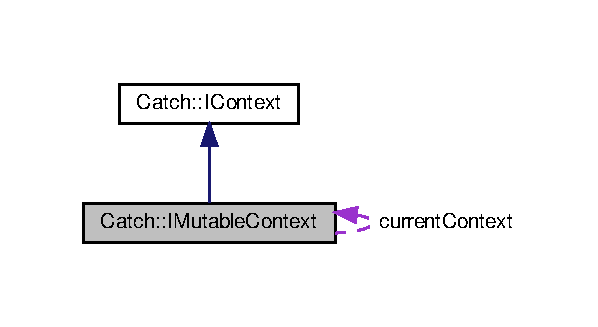
\includegraphics[width=287pt]{structCatch_1_1IMutableContext__coll__graph}
\end{center}
\end{figure}
\subsection*{Public Member Functions}
\begin{DoxyCompactItemize}
\item 
\mbox{\Hypertarget{structCatch_1_1IMutableContext_a4a80afd0525b7def21bee8d9b48f2d39}\label{structCatch_1_1IMutableContext_a4a80afd0525b7def21bee8d9b48f2d39}} 
virtual void {\bfseries set\+Result\+Capture} (\hyperlink{structCatch_1_1IResultCapture}{I\+Result\+Capture} $\ast$result\+Capture)=0
\item 
\mbox{\Hypertarget{structCatch_1_1IMutableContext_af2e53b1dea4527a2587cff266a730f6e}\label{structCatch_1_1IMutableContext_af2e53b1dea4527a2587cff266a730f6e}} 
virtual void {\bfseries set\+Runner} (\hyperlink{structCatch_1_1IRunner}{I\+Runner} $\ast$runner)=0
\item 
\mbox{\Hypertarget{structCatch_1_1IMutableContext_aa81ba080fce084e9482f20338bc88531}\label{structCatch_1_1IMutableContext_aa81ba080fce084e9482f20338bc88531}} 
virtual void {\bfseries set\+Config} (I\+Config\+Ptr const \&config)=0
\end{DoxyCompactItemize}
\subsection*{Static Private Member Functions}
\begin{DoxyCompactItemize}
\item 
\mbox{\Hypertarget{structCatch_1_1IMutableContext_a17e4b3f9a9674af7e2c4f081c692a628}\label{structCatch_1_1IMutableContext_a17e4b3f9a9674af7e2c4f081c692a628}} 
static void {\bfseries create\+Context} ()
\end{DoxyCompactItemize}
\subsection*{Static Private Attributes}
\begin{DoxyCompactItemize}
\item 
\mbox{\Hypertarget{structCatch_1_1IMutableContext_aca4de034d0deed74dba34f143e4e273e}\label{structCatch_1_1IMutableContext_aca4de034d0deed74dba34f143e4e273e}} 
static \hyperlink{structCatch_1_1IMutableContext}{I\+Mutable\+Context} $\ast$ {\bfseries current\+Context}
\end{DoxyCompactItemize}
\subsection*{Friends}
\begin{DoxyCompactItemize}
\item 
\mbox{\Hypertarget{structCatch_1_1IMutableContext_aea4b25692aaf4397cdf630716976f6b8}\label{structCatch_1_1IMutableContext_aea4b25692aaf4397cdf630716976f6b8}} 
\hyperlink{structCatch_1_1IMutableContext}{I\+Mutable\+Context} \& {\bfseries get\+Current\+Mutable\+Context} ()
\item 
\mbox{\Hypertarget{structCatch_1_1IMutableContext_ac07cdb7d744cc8f09672d924324b55fd}\label{structCatch_1_1IMutableContext_ac07cdb7d744cc8f09672d924324b55fd}} 
void {\bfseries clean\+Up\+Context} ()
\end{DoxyCompactItemize}


The documentation for this struct was generated from the following file\+:\begin{DoxyCompactItemize}
\item 
/home/sinflair/\+P/crypto/\+A\+K/src/\+Praktikum-\/\+D\+E\+S/catch.\+hpp\end{DoxyCompactItemize}

\hypertarget{structCatch_1_1IMutableEnumValuesRegistry}{}\section{Catch\+:\+:I\+Mutable\+Enum\+Values\+Registry Struct Reference}
\label{structCatch_1_1IMutableEnumValuesRegistry}\index{Catch\+::\+I\+Mutable\+Enum\+Values\+Registry@{Catch\+::\+I\+Mutable\+Enum\+Values\+Registry}}
\subsection*{Public Member Functions}
\begin{DoxyCompactItemize}
\item 
\mbox{\Hypertarget{structCatch_1_1IMutableEnumValuesRegistry_a948e66e85f5b66ab68256d50bfe548f4}\label{structCatch_1_1IMutableEnumValuesRegistry_a948e66e85f5b66ab68256d50bfe548f4}} 
virtual \hyperlink{structCatch_1_1Detail_1_1EnumInfo}{Detail\+::\+Enum\+Info} const  \& {\bfseries register\+Enum} (\hyperlink{classCatch_1_1StringRef}{String\+Ref} enum\+Name, \hyperlink{classCatch_1_1StringRef}{String\+Ref} all\+Enums, std\+::vector$<$ int $>$ const \&values)=0
\item 
\mbox{\Hypertarget{structCatch_1_1IMutableEnumValuesRegistry_a60e4546c6fd45f9be68e43410403b562}\label{structCatch_1_1IMutableEnumValuesRegistry_a60e4546c6fd45f9be68e43410403b562}} 
{\footnotesize template$<$typename E $>$ }\\\hyperlink{structCatch_1_1Detail_1_1EnumInfo}{Detail\+::\+Enum\+Info} const  \& {\bfseries register\+Enum} (\hyperlink{classCatch_1_1StringRef}{String\+Ref} enum\+Name, \hyperlink{classCatch_1_1StringRef}{String\+Ref} all\+Enums, std\+::initializer\+\_\+list$<$ E $>$ values)
\end{DoxyCompactItemize}


The documentation for this struct was generated from the following file\+:\begin{DoxyCompactItemize}
\item 
/home/sinflair/\+P/crypto/\+A\+K/src/\+Praktikum-\/\+D\+E\+S/catch.\+hpp\end{DoxyCompactItemize}

\hypertarget{structCatch_1_1IMutableRegistryHub}{}\section{Catch\+:\+:I\+Mutable\+Registry\+Hub Struct Reference}
\label{structCatch_1_1IMutableRegistryHub}\index{Catch\+::\+I\+Mutable\+Registry\+Hub@{Catch\+::\+I\+Mutable\+Registry\+Hub}}
\subsection*{Public Member Functions}
\begin{DoxyCompactItemize}
\item 
\mbox{\Hypertarget{structCatch_1_1IMutableRegistryHub_a1c0ac202ac31ee9f88e8ff5cbac4b243}\label{structCatch_1_1IMutableRegistryHub_a1c0ac202ac31ee9f88e8ff5cbac4b243}} 
virtual void {\bfseries register\+Reporter} (std\+::string const \&name, I\+Reporter\+Factory\+Ptr const \&factory)=0
\item 
\mbox{\Hypertarget{structCatch_1_1IMutableRegistryHub_abd892a133f85581fd00ee75bb379ca56}\label{structCatch_1_1IMutableRegistryHub_abd892a133f85581fd00ee75bb379ca56}} 
virtual void {\bfseries register\+Listener} (I\+Reporter\+Factory\+Ptr const \&factory)=0
\item 
\mbox{\Hypertarget{structCatch_1_1IMutableRegistryHub_a11b85c6744d88c9f83fe16ad4a8dd451}\label{structCatch_1_1IMutableRegistryHub_a11b85c6744d88c9f83fe16ad4a8dd451}} 
virtual void {\bfseries register\+Test} (\hyperlink{classCatch_1_1TestCase}{Test\+Case} const \&test\+Info)=0
\item 
\mbox{\Hypertarget{structCatch_1_1IMutableRegistryHub_ae6825365102693cf7707db022a2c2b49}\label{structCatch_1_1IMutableRegistryHub_ae6825365102693cf7707db022a2c2b49}} 
virtual void {\bfseries register\+Translator} (const \hyperlink{structCatch_1_1IExceptionTranslator}{I\+Exception\+Translator} $\ast$translator)=0
\item 
\mbox{\Hypertarget{structCatch_1_1IMutableRegistryHub_abf2e386b6f94f615719ada711adbf822}\label{structCatch_1_1IMutableRegistryHub_abf2e386b6f94f615719ada711adbf822}} 
virtual void {\bfseries register\+Tag\+Alias} (std\+::string const \&alias, std\+::string const \&tag, \hyperlink{structCatch_1_1SourceLineInfo}{Source\+Line\+Info} const \&line\+Info)=0
\item 
\mbox{\Hypertarget{structCatch_1_1IMutableRegistryHub_a72a7d5386851ac3200f8da794a009c86}\label{structCatch_1_1IMutableRegistryHub_a72a7d5386851ac3200f8da794a009c86}} 
virtual void {\bfseries register\+Startup\+Exception} () noexcept=0
\item 
\mbox{\Hypertarget{structCatch_1_1IMutableRegistryHub_ab91c4fd63eeb0efd9bfb270e8bbd231d}\label{structCatch_1_1IMutableRegistryHub_ab91c4fd63eeb0efd9bfb270e8bbd231d}} 
virtual \hyperlink{structCatch_1_1IMutableEnumValuesRegistry}{I\+Mutable\+Enum\+Values\+Registry} \& {\bfseries get\+Mutable\+Enum\+Values\+Registry} ()=0
\end{DoxyCompactItemize}


The documentation for this struct was generated from the following file\+:\begin{DoxyCompactItemize}
\item 
/home/sinflair/\+P/crypto/\+A\+K/src/\+Praktikum-\/\+D\+E\+S/catch.\+hpp\end{DoxyCompactItemize}

\hypertarget{structCatch_1_1IRegistryHub}{}\section{Catch\+:\+:I\+Registry\+Hub Struct Reference}
\label{structCatch_1_1IRegistryHub}\index{Catch\+::\+I\+Registry\+Hub@{Catch\+::\+I\+Registry\+Hub}}
\subsection*{Public Member Functions}
\begin{DoxyCompactItemize}
\item 
\mbox{\Hypertarget{structCatch_1_1IRegistryHub_a55534563f7ecf7e20ec1e37285ebe54d}\label{structCatch_1_1IRegistryHub_a55534563f7ecf7e20ec1e37285ebe54d}} 
virtual I\+Reporter\+Registry const  \& {\bfseries get\+Reporter\+Registry} () const =0
\item 
\mbox{\Hypertarget{structCatch_1_1IRegistryHub_af4f6255f0c0f8f1f179fa9d7d4843076}\label{structCatch_1_1IRegistryHub_af4f6255f0c0f8f1f179fa9d7d4843076}} 
virtual \hyperlink{structCatch_1_1ITestCaseRegistry}{I\+Test\+Case\+Registry} const  \& {\bfseries get\+Test\+Case\+Registry} () const =0
\item 
\mbox{\Hypertarget{structCatch_1_1IRegistryHub_a3c511b1d33e5a6d95c333a0ff387df1a}\label{structCatch_1_1IRegistryHub_a3c511b1d33e5a6d95c333a0ff387df1a}} 
virtual I\+Tag\+Alias\+Registry const  \& {\bfseries get\+Tag\+Alias\+Registry} () const =0
\item 
\mbox{\Hypertarget{structCatch_1_1IRegistryHub_a48347c170d9c583af73027a27b2f0bd4}\label{structCatch_1_1IRegistryHub_a48347c170d9c583af73027a27b2f0bd4}} 
virtual \hyperlink{structCatch_1_1IExceptionTranslatorRegistry}{I\+Exception\+Translator\+Registry} const  \& {\bfseries get\+Exception\+Translator\+Registry} () const =0
\item 
\mbox{\Hypertarget{structCatch_1_1IRegistryHub_a00281210628e6c616aca1d3e0d84db04}\label{structCatch_1_1IRegistryHub_a00281210628e6c616aca1d3e0d84db04}} 
virtual Startup\+Exception\+Registry const  \& {\bfseries get\+Startup\+Exception\+Registry} () const =0
\end{DoxyCompactItemize}


The documentation for this struct was generated from the following file\+:\begin{DoxyCompactItemize}
\item 
/home/sinflair/\+P/crypto/\+A\+K/src/\+Praktikum-\/\+D\+E\+S/catch.\+hpp\end{DoxyCompactItemize}

\hypertarget{structCatch_1_1IResultCapture}{}\section{Catch\+:\+:I\+Result\+Capture Struct Reference}
\label{structCatch_1_1IResultCapture}\index{Catch\+::\+I\+Result\+Capture@{Catch\+::\+I\+Result\+Capture}}
\subsection*{Public Member Functions}
\begin{DoxyCompactItemize}
\item 
\mbox{\Hypertarget{structCatch_1_1IResultCapture_a5b76ed52badcb64cf374202e12b81a03}\label{structCatch_1_1IResultCapture_a5b76ed52badcb64cf374202e12b81a03}} 
virtual bool {\bfseries section\+Started} (\hyperlink{structCatch_1_1SectionInfo}{Section\+Info} const \&section\+Info, \hyperlink{structCatch_1_1Counts}{Counts} \&assertions)=0
\item 
\mbox{\Hypertarget{structCatch_1_1IResultCapture_a4e152bc43dc0933684e31fa67a58195d}\label{structCatch_1_1IResultCapture_a4e152bc43dc0933684e31fa67a58195d}} 
virtual void {\bfseries section\+Ended} (\hyperlink{structCatch_1_1SectionEndInfo}{Section\+End\+Info} const \&end\+Info)=0
\item 
\mbox{\Hypertarget{structCatch_1_1IResultCapture_afcc71eef8ca821ae132cced4a2be6988}\label{structCatch_1_1IResultCapture_afcc71eef8ca821ae132cced4a2be6988}} 
virtual void {\bfseries section\+Ended\+Early} (\hyperlink{structCatch_1_1SectionEndInfo}{Section\+End\+Info} const \&end\+Info)=0
\item 
\mbox{\Hypertarget{structCatch_1_1IResultCapture_ab020d111e29ad1cabe1227dcfda712ef}\label{structCatch_1_1IResultCapture_ab020d111e29ad1cabe1227dcfda712ef}} 
virtual auto {\bfseries acquire\+Generator\+Tracker} (\hyperlink{structCatch_1_1SourceLineInfo}{Source\+Line\+Info} const \&line\+Info) -\/$>$ \hyperlink{structCatch_1_1IGeneratorTracker}{I\+Generator\+Tracker} \&=0
\item 
\mbox{\Hypertarget{structCatch_1_1IResultCapture_a91d154c1e087e383dcde5aad95cb6a05}\label{structCatch_1_1IResultCapture_a91d154c1e087e383dcde5aad95cb6a05}} 
virtual void {\bfseries push\+Scoped\+Message} (\hyperlink{structCatch_1_1MessageInfo}{Message\+Info} const \&message)=0
\item 
\mbox{\Hypertarget{structCatch_1_1IResultCapture_a42bcb13276706bf8c3ce081ce16d37fd}\label{structCatch_1_1IResultCapture_a42bcb13276706bf8c3ce081ce16d37fd}} 
virtual void {\bfseries pop\+Scoped\+Message} (\hyperlink{structCatch_1_1MessageInfo}{Message\+Info} const \&message)=0
\item 
\mbox{\Hypertarget{structCatch_1_1IResultCapture_a49f74f1323ef8be71b8f9b8e8b2c0fc2}\label{structCatch_1_1IResultCapture_a49f74f1323ef8be71b8f9b8e8b2c0fc2}} 
virtual void {\bfseries emplace\+Unscoped\+Message} (\hyperlink{structCatch_1_1MessageBuilder}{Message\+Builder} const \&builder)=0
\item 
\mbox{\Hypertarget{structCatch_1_1IResultCapture_a48559e6598ba9474b903697b69c769b2}\label{structCatch_1_1IResultCapture_a48559e6598ba9474b903697b69c769b2}} 
virtual void {\bfseries handle\+Fatal\+Error\+Condition} (\hyperlink{classCatch_1_1StringRef}{String\+Ref} message)=0
\item 
\mbox{\Hypertarget{structCatch_1_1IResultCapture_a59a2b05391e464954575d2afb6d5d607}\label{structCatch_1_1IResultCapture_a59a2b05391e464954575d2afb6d5d607}} 
virtual void {\bfseries handle\+Expr} (\hyperlink{structCatch_1_1AssertionInfo}{Assertion\+Info} const \&info, \hyperlink{structCatch_1_1ITransientExpression}{I\+Transient\+Expression} const \&expr, \hyperlink{structCatch_1_1AssertionReaction}{Assertion\+Reaction} \&reaction)=0
\item 
\mbox{\Hypertarget{structCatch_1_1IResultCapture_a21788ebc64571abf322b80c8cc51794d}\label{structCatch_1_1IResultCapture_a21788ebc64571abf322b80c8cc51794d}} 
virtual void {\bfseries handle\+Message} (\hyperlink{structCatch_1_1AssertionInfo}{Assertion\+Info} const \&info, Result\+Was\+::\+Of\+Type result\+Type, \hyperlink{classCatch_1_1StringRef}{String\+Ref} const \&message, \hyperlink{structCatch_1_1AssertionReaction}{Assertion\+Reaction} \&reaction)=0
\item 
\mbox{\Hypertarget{structCatch_1_1IResultCapture_a6382ed20486e2d9a020da971c6d5c53d}\label{structCatch_1_1IResultCapture_a6382ed20486e2d9a020da971c6d5c53d}} 
virtual void {\bfseries handle\+Unexpected\+Exception\+Not\+Thrown} (\hyperlink{structCatch_1_1AssertionInfo}{Assertion\+Info} const \&info, \hyperlink{structCatch_1_1AssertionReaction}{Assertion\+Reaction} \&reaction)=0
\item 
\mbox{\Hypertarget{structCatch_1_1IResultCapture_afc97bc69829185222f955ebeef97adfe}\label{structCatch_1_1IResultCapture_afc97bc69829185222f955ebeef97adfe}} 
virtual void {\bfseries handle\+Unexpected\+Inflight\+Exception} (\hyperlink{structCatch_1_1AssertionInfo}{Assertion\+Info} const \&info, std\+::string const \&message, \hyperlink{structCatch_1_1AssertionReaction}{Assertion\+Reaction} \&reaction)=0
\item 
\mbox{\Hypertarget{structCatch_1_1IResultCapture_a89b89372eb09cc44f8dcad363de6157d}\label{structCatch_1_1IResultCapture_a89b89372eb09cc44f8dcad363de6157d}} 
virtual void {\bfseries handle\+Incomplete} (\hyperlink{structCatch_1_1AssertionInfo}{Assertion\+Info} const \&info)=0
\item 
\mbox{\Hypertarget{structCatch_1_1IResultCapture_ab7dbdf8aa28427119583e24dbb302c63}\label{structCatch_1_1IResultCapture_ab7dbdf8aa28427119583e24dbb302c63}} 
virtual void {\bfseries handle\+Non\+Expr} (\hyperlink{structCatch_1_1AssertionInfo}{Assertion\+Info} const \&info, Result\+Was\+::\+Of\+Type result\+Type, \hyperlink{structCatch_1_1AssertionReaction}{Assertion\+Reaction} \&reaction)=0
\item 
\mbox{\Hypertarget{structCatch_1_1IResultCapture_a973435fbdcb2f6f07a0ec5719a01e956}\label{structCatch_1_1IResultCapture_a973435fbdcb2f6f07a0ec5719a01e956}} 
virtual bool {\bfseries last\+Assertion\+Passed} ()=0
\item 
\mbox{\Hypertarget{structCatch_1_1IResultCapture_a9b0ef2cb071e9a9dc6ec1b533026aea7}\label{structCatch_1_1IResultCapture_a9b0ef2cb071e9a9dc6ec1b533026aea7}} 
virtual void {\bfseries assertion\+Passed} ()=0
\item 
\mbox{\Hypertarget{structCatch_1_1IResultCapture_aea1617f4a84cc648246aa3ed6918b5bf}\label{structCatch_1_1IResultCapture_aea1617f4a84cc648246aa3ed6918b5bf}} 
virtual std\+::string {\bfseries get\+Current\+Test\+Name} () const =0
\item 
\mbox{\Hypertarget{structCatch_1_1IResultCapture_ab18872c89fab97405a56e9c6a4919736}\label{structCatch_1_1IResultCapture_ab18872c89fab97405a56e9c6a4919736}} 
virtual const Assertion\+Result $\ast$ {\bfseries get\+Last\+Result} () const =0
\item 
\mbox{\Hypertarget{structCatch_1_1IResultCapture_ae63ecec95db4c236c63ecf616f483810}\label{structCatch_1_1IResultCapture_ae63ecec95db4c236c63ecf616f483810}} 
virtual void {\bfseries exception\+Early\+Reported} ()=0
\end{DoxyCompactItemize}


The documentation for this struct was generated from the following file\+:\begin{DoxyCompactItemize}
\item 
/home/sinflair/\+P/crypto/\+A\+K/src/\+Praktikum-\/\+D\+E\+S/catch.\+hpp\end{DoxyCompactItemize}

\hypertarget{structCatch_1_1IRunner}{}\section{Catch\+:\+:I\+Runner Struct Reference}
\label{structCatch_1_1IRunner}\index{Catch\+::\+I\+Runner@{Catch\+::\+I\+Runner}}
\subsection*{Public Member Functions}
\begin{DoxyCompactItemize}
\item 
\mbox{\Hypertarget{structCatch_1_1IRunner_a03713202dd2e041e30b8030088ab0116}\label{structCatch_1_1IRunner_a03713202dd2e041e30b8030088ab0116}} 
virtual bool {\bfseries aborting} () const =0
\end{DoxyCompactItemize}


The documentation for this struct was generated from the following file\+:\begin{DoxyCompactItemize}
\item 
/home/sinflair/\+P/crypto/\+A\+K/src/\+Praktikum-\/\+D\+E\+S/catch.\+hpp\end{DoxyCompactItemize}

\hypertarget{structCatch_1_1is__callable}{}\section{Catch\+:\+:is\+\_\+callable$<$ T $>$ Struct Template Reference}
\label{structCatch_1_1is__callable}\index{Catch\+::is\+\_\+callable$<$ T $>$@{Catch\+::is\+\_\+callable$<$ T $>$}}


The documentation for this struct was generated from the following file\+:\begin{DoxyCompactItemize}
\item 
/home/sinflair/\+P/crypto/\+A\+K/src/\+Praktikum-\/\+D\+E\+S/catch.\+hpp\end{DoxyCompactItemize}

\hypertarget{structCatch_1_1is__callable_3_01Fun_07Args_8_8_8_08_4}{}\section{Catch\+:\+:is\+\_\+callable$<$ Fun(Args...)$>$ Struct Template Reference}
\label{structCatch_1_1is__callable_3_01Fun_07Args_8_8_8_08_4}\index{Catch\+::is\+\_\+callable$<$ Fun(\+Args...)$>$@{Catch\+::is\+\_\+callable$<$ Fun(\+Args...)$>$}}


Inheritance diagram for Catch\+:\+:is\+\_\+callable$<$ Fun(Args...)$>$\+:
\nopagebreak
\begin{figure}[H]
\begin{center}
\leavevmode
\includegraphics[width=179pt]{structCatch_1_1is__callable_3_01Fun_07Args_8_8_8_08_4__inherit__graph}
\end{center}
\end{figure}


Collaboration diagram for Catch\+:\+:is\+\_\+callable$<$ Fun(Args...)$>$\+:
\nopagebreak
\begin{figure}[H]
\begin{center}
\leavevmode
\includegraphics[width=179pt]{structCatch_1_1is__callable_3_01Fun_07Args_8_8_8_08_4__coll__graph}
\end{center}
\end{figure}


The documentation for this struct was generated from the following file\+:\begin{DoxyCompactItemize}
\item 
/home/sinflair/\+P/crypto/\+A\+K/src/\+Praktikum-\/\+D\+E\+S/catch.\+hpp\end{DoxyCompactItemize}

\hypertarget{structCatch_1_1is__callable__tester}{}\section{Catch\+:\+:is\+\_\+callable\+\_\+tester Struct Reference}
\label{structCatch_1_1is__callable__tester}\index{Catch\+::is\+\_\+callable\+\_\+tester@{Catch\+::is\+\_\+callable\+\_\+tester}}
\subsection*{Static Public Member Functions}
\begin{DoxyCompactItemize}
\item 
\mbox{\Hypertarget{structCatch_1_1is__callable__tester_a91c513c4fc18b01b96fa0132706f34b3}\label{structCatch_1_1is__callable__tester_a91c513c4fc18b01b96fa0132706f34b3}} 
{\footnotesize template$<$typename Fun , typename... Args$>$ }\\static \hyperlink{structCatch_1_1true__given}{true\+\_\+given}$<$ decltype(std\+::declval$<$ Fun $>$)(std\+::declval$<$ Args $>$)...))$>$ {\bfseries test} (int)
\item 
\mbox{\Hypertarget{structCatch_1_1is__callable__tester_adce16c4accb860bf46f6491dd70cfd63}\label{structCatch_1_1is__callable__tester_adce16c4accb860bf46f6491dd70cfd63}} 
{\footnotesize template$<$typename... $>$ }\\static std\+::false\+\_\+type {\bfseries test} (...)
\end{DoxyCompactItemize}


The documentation for this struct was generated from the following file\+:\begin{DoxyCompactItemize}
\item 
/home/sinflair/\+P/crypto/\+A\+K/src/\+Praktikum-\/\+D\+E\+S/catch.\+hpp\end{DoxyCompactItemize}

\hypertarget{structCatch_1_1is__range}{}\section{Catch\+:\+:is\+\_\+range$<$ T $>$ Struct Template Reference}
\label{structCatch_1_1is__range}\index{Catch\+::is\+\_\+range$<$ T $>$@{Catch\+::is\+\_\+range$<$ T $>$}}
\subsection*{Static Public Attributes}
\begin{DoxyCompactItemize}
\item 
static const bool {\bfseries value}
\end{DoxyCompactItemize}


\subsection{Member Data Documentation}
\mbox{\Hypertarget{structCatch_1_1is__range_afaec39e819c3956829cbbd00feba11be}\label{structCatch_1_1is__range_afaec39e819c3956829cbbd00feba11be}} 
\index{Catch\+::is\+\_\+range@{Catch\+::is\+\_\+range}!value@{value}}
\index{value@{value}!Catch\+::is\+\_\+range@{Catch\+::is\+\_\+range}}
\subsubsection{\texorpdfstring{value}{value}}
{\footnotesize\ttfamily template$<$typename T $>$ \\
const bool \hyperlink{structCatch_1_1is__range}{Catch\+::is\+\_\+range}$<$ T $>$\+::value\hspace{0.3cm}{\ttfamily [static]}}

{\bfseries Initial value\+:}
\begin{DoxyCode}
=
!std::is\_same<decltype(begin(std::declval<T>())), not\_this\_one>::value &&
!std::is\_same<decltype(end(std::declval<T>())), not\_this\_one>::value
\end{DoxyCode}


The documentation for this struct was generated from the following file\+:\begin{DoxyCompactItemize}
\item 
/home/sinflair/\+P/crypto/\+A\+K/src/\+Praktikum-\/\+D\+E\+S/catch.\+hpp\end{DoxyCompactItemize}

\hypertarget{classCatch_1_1Detail_1_1IsStreamInsertable}{}\section{Catch\+:\+:Detail\+:\+:Is\+Stream\+Insertable$<$ T $>$ Class Template Reference}
\label{classCatch_1_1Detail_1_1IsStreamInsertable}\index{Catch\+::\+Detail\+::\+Is\+Stream\+Insertable$<$ T $>$@{Catch\+::\+Detail\+::\+Is\+Stream\+Insertable$<$ T $>$}}
\subsection*{Static Public Attributes}
\begin{DoxyCompactItemize}
\item 
\mbox{\Hypertarget{classCatch_1_1Detail_1_1IsStreamInsertable_a42818b09ae5851126a70ee263769e309}\label{classCatch_1_1Detail_1_1IsStreamInsertable_a42818b09ae5851126a70ee263769e309}} 
static const bool {\bfseries value} = decltype(test$<$std\+::ostream, const T\&$>$(0))\+::value
\end{DoxyCompactItemize}
\subsection*{Static Private Member Functions}
\begin{DoxyCompactItemize}
\item 
\mbox{\Hypertarget{classCatch_1_1Detail_1_1IsStreamInsertable_a921c9480534008707cc6bbe5545acffe}\label{classCatch_1_1Detail_1_1IsStreamInsertable_a921c9480534008707cc6bbe5545acffe}} 
{\footnotesize template$<$typename Stream , typename U $>$ }\\static auto {\bfseries test} (int) -\/$>$ decltype(std\+::declval$<$ Stream \&$>$()$<$$<$ std\+::declval$<$ U $>$(), std\+::true\+\_\+type())
\item 
\mbox{\Hypertarget{classCatch_1_1Detail_1_1IsStreamInsertable_ac5761375646929916dc5e165d44cd3d9}\label{classCatch_1_1Detail_1_1IsStreamInsertable_ac5761375646929916dc5e165d44cd3d9}} 
{\footnotesize template$<$typename , typename $>$ }\\static auto {\bfseries test} (...) -\/$>$ std\+::false\+\_\+type
\end{DoxyCompactItemize}


The documentation for this class was generated from the following file\+:\begin{DoxyCompactItemize}
\item 
/home/sinflair/\+P/crypto/\+A\+K/src/\+Praktikum-\/\+D\+E\+S/catch.\+hpp\end{DoxyCompactItemize}

\hypertarget{structCatch_1_1IStream}{}\section{Catch\+:\+:I\+Stream Struct Reference}
\label{structCatch_1_1IStream}\index{Catch\+::\+I\+Stream@{Catch\+::\+I\+Stream}}
\subsection*{Public Member Functions}
\begin{DoxyCompactItemize}
\item 
\mbox{\Hypertarget{structCatch_1_1IStream_a55a9ddbe250261ff38642f480ebdd902}\label{structCatch_1_1IStream_a55a9ddbe250261ff38642f480ebdd902}} 
virtual std\+::ostream \& {\bfseries stream} () const =0
\end{DoxyCompactItemize}


The documentation for this struct was generated from the following file\+:\begin{DoxyCompactItemize}
\item 
/home/sinflair/\+P/crypto/\+A\+K/src/\+Praktikum-\/\+D\+E\+S/catch.\+hpp\end{DoxyCompactItemize}

\hypertarget{classCatch_1_1Generators_1_1IteratorGenerator}{}\section{Catch\+:\+:Generators\+:\+:Iterator\+Generator$<$ T $>$ Class Template Reference}
\label{classCatch_1_1Generators_1_1IteratorGenerator}\index{Catch\+::\+Generators\+::\+Iterator\+Generator$<$ T $>$@{Catch\+::\+Generators\+::\+Iterator\+Generator$<$ T $>$}}


Inheritance diagram for Catch\+:\+:Generators\+:\+:Iterator\+Generator$<$ T $>$\+:
\nopagebreak
\begin{figure}[H]
\begin{center}
\leavevmode
\includegraphics[width=199pt]{classCatch_1_1Generators_1_1IteratorGenerator__inherit__graph}
\end{center}
\end{figure}


Collaboration diagram for Catch\+:\+:Generators\+:\+:Iterator\+Generator$<$ T $>$\+:
\nopagebreak
\begin{figure}[H]
\begin{center}
\leavevmode
\includegraphics[width=199pt]{classCatch_1_1Generators_1_1IteratorGenerator__coll__graph}
\end{center}
\end{figure}
\subsection*{Public Member Functions}
\begin{DoxyCompactItemize}
\item 
\mbox{\Hypertarget{classCatch_1_1Generators_1_1IteratorGenerator_a1f795b1bbd515274673115c0a9fc2e54}\label{classCatch_1_1Generators_1_1IteratorGenerator_a1f795b1bbd515274673115c0a9fc2e54}} 
{\footnotesize template$<$typename Input\+Iterator , typename Input\+Sentinel $>$ }\\{\bfseries Iterator\+Generator} (Input\+Iterator first, Input\+Sentinel last)
\item 
\mbox{\Hypertarget{classCatch_1_1Generators_1_1IteratorGenerator_a61688118e5caba23340b4b949c3bb7e4}\label{classCatch_1_1Generators_1_1IteratorGenerator_a61688118e5caba23340b4b949c3bb7e4}} 
T const  \& {\bfseries get} () const override
\item 
\mbox{\Hypertarget{classCatch_1_1Generators_1_1IteratorGenerator_acafb4fa1eebe5e1db571621a35a3f137}\label{classCatch_1_1Generators_1_1IteratorGenerator_acafb4fa1eebe5e1db571621a35a3f137}} 
bool {\bfseries next} () override
\end{DoxyCompactItemize}
\subsection*{Private Attributes}
\begin{DoxyCompactItemize}
\item 
\mbox{\Hypertarget{classCatch_1_1Generators_1_1IteratorGenerator_a74eb1a6990cf0e3b548e8654bd6e99ef}\label{classCatch_1_1Generators_1_1IteratorGenerator_a74eb1a6990cf0e3b548e8654bd6e99ef}} 
std\+::vector$<$ T $>$ {\bfseries m\+\_\+elems}
\item 
\mbox{\Hypertarget{classCatch_1_1Generators_1_1IteratorGenerator_a43b70e3cf312294219bd2485eaa75ba1}\label{classCatch_1_1Generators_1_1IteratorGenerator_a43b70e3cf312294219bd2485eaa75ba1}} 
size\+\_\+t {\bfseries m\+\_\+current} = 0
\end{DoxyCompactItemize}
\subsection*{Additional Inherited Members}


The documentation for this class was generated from the following file\+:\begin{DoxyCompactItemize}
\item 
/home/sinflair/\+P/crypto/\+A\+K/src/\+Praktikum-\/\+D\+E\+S/catch.\+hpp\end{DoxyCompactItemize}

\hypertarget{structCatch_1_1ITestCaseRegistry}{}\section{Catch\+:\+:I\+Test\+Case\+Registry Struct Reference}
\label{structCatch_1_1ITestCaseRegistry}\index{Catch\+::\+I\+Test\+Case\+Registry@{Catch\+::\+I\+Test\+Case\+Registry}}
\subsection*{Public Member Functions}
\begin{DoxyCompactItemize}
\item 
\mbox{\Hypertarget{structCatch_1_1ITestCaseRegistry_ad6e4d4a621655123f73ae98cfeda063d}\label{structCatch_1_1ITestCaseRegistry_ad6e4d4a621655123f73ae98cfeda063d}} 
virtual std\+::vector$<$ \hyperlink{classCatch_1_1TestCase}{Test\+Case} $>$ const  \& {\bfseries get\+All\+Tests} () const =0
\item 
\mbox{\Hypertarget{structCatch_1_1ITestCaseRegistry_a33e46639d0319d35497c05bb5d02be5a}\label{structCatch_1_1ITestCaseRegistry_a33e46639d0319d35497c05bb5d02be5a}} 
virtual std\+::vector$<$ \hyperlink{classCatch_1_1TestCase}{Test\+Case} $>$ const  \& {\bfseries get\+All\+Tests\+Sorted} (\hyperlink{structCatch_1_1IConfig}{I\+Config} const \&config) const =0
\end{DoxyCompactItemize}


The documentation for this struct was generated from the following file\+:\begin{DoxyCompactItemize}
\item 
/home/sinflair/\+P/crypto/\+A\+K/src/\+Praktikum-\/\+D\+E\+S/catch.\+hpp\end{DoxyCompactItemize}

\hypertarget{structCatch_1_1ITestInvoker}{}\section{Catch\+:\+:I\+Test\+Invoker Struct Reference}
\label{structCatch_1_1ITestInvoker}\index{Catch\+::\+I\+Test\+Invoker@{Catch\+::\+I\+Test\+Invoker}}


Inheritance diagram for Catch\+:\+:I\+Test\+Invoker\+:
\nopagebreak
\begin{figure}[H]
\begin{center}
\leavevmode
\includegraphics[width=250pt]{structCatch_1_1ITestInvoker__inherit__graph}
\end{center}
\end{figure}
\subsection*{Public Member Functions}
\begin{DoxyCompactItemize}
\item 
\mbox{\Hypertarget{structCatch_1_1ITestInvoker_a6fcd5c5b67d6d5ade6491ff33411ca7f}\label{structCatch_1_1ITestInvoker_a6fcd5c5b67d6d5ade6491ff33411ca7f}} 
virtual void {\bfseries invoke} () const =0
\end{DoxyCompactItemize}


The documentation for this struct was generated from the following file\+:\begin{DoxyCompactItemize}
\item 
/home/sinflair/\+P/crypto/\+A\+K/src/\+Praktikum-\/\+D\+E\+S/catch.\+hpp\end{DoxyCompactItemize}

\hypertarget{structCatch_1_1ITransientExpression}{}\section{Catch\+:\+:I\+Transient\+Expression Struct Reference}
\label{structCatch_1_1ITransientExpression}\index{Catch\+::\+I\+Transient\+Expression@{Catch\+::\+I\+Transient\+Expression}}


Inheritance diagram for Catch\+:\+:I\+Transient\+Expression\+:
\nopagebreak
\begin{figure}[H]
\begin{center}
\leavevmode
\includegraphics[width=350pt]{structCatch_1_1ITransientExpression__inherit__graph}
\end{center}
\end{figure}
\subsection*{Public Member Functions}
\begin{DoxyCompactItemize}
\item 
\mbox{\Hypertarget{structCatch_1_1ITransientExpression_a3b436e13a0a6d3522bbf70d4e31deb22}\label{structCatch_1_1ITransientExpression_a3b436e13a0a6d3522bbf70d4e31deb22}} 
auto {\bfseries is\+Binary\+Expression} () const -\/$>$ bool
\item 
\mbox{\Hypertarget{structCatch_1_1ITransientExpression_a101c7db86c87eff93a8ff496720e6320}\label{structCatch_1_1ITransientExpression_a101c7db86c87eff93a8ff496720e6320}} 
auto {\bfseries get\+Result} () const -\/$>$ bool
\item 
\mbox{\Hypertarget{structCatch_1_1ITransientExpression_aabe1889df9c6e639a24afb08d8a0fe9e}\label{structCatch_1_1ITransientExpression_aabe1889df9c6e639a24afb08d8a0fe9e}} 
virtual void {\bfseries stream\+Reconstructed\+Expression} (std\+::ostream \&os) const =0
\item 
\mbox{\Hypertarget{structCatch_1_1ITransientExpression_aafe69572b7ed884e63ec81f58d4afd8c}\label{structCatch_1_1ITransientExpression_aafe69572b7ed884e63ec81f58d4afd8c}} 
{\bfseries I\+Transient\+Expression} (bool is\+Binary\+Expression, bool result)
\end{DoxyCompactItemize}
\subsection*{Public Attributes}
\begin{DoxyCompactItemize}
\item 
\mbox{\Hypertarget{structCatch_1_1ITransientExpression_a75ce48da824d514d08152d396abb28d8}\label{structCatch_1_1ITransientExpression_a75ce48da824d514d08152d396abb28d8}} 
bool {\bfseries m\+\_\+is\+Binary\+Expression}
\item 
\mbox{\Hypertarget{structCatch_1_1ITransientExpression_a4646e2b5e0156e913653ec3b9b60c942}\label{structCatch_1_1ITransientExpression_a4646e2b5e0156e913653ec3b9b60c942}} 
bool {\bfseries m\+\_\+result}
\end{DoxyCompactItemize}


The documentation for this struct was generated from the following file\+:\begin{DoxyCompactItemize}
\item 
/home/sinflair/\+P/crypto/\+A\+K/src/\+Praktikum-\/\+D\+E\+S/catch.\+hpp\end{DoxyCompactItemize}

\hypertarget{classCatch_1_1LazyExpression}{}\section{Catch\+:\+:Lazy\+Expression Class Reference}
\label{classCatch_1_1LazyExpression}\index{Catch\+::\+Lazy\+Expression@{Catch\+::\+Lazy\+Expression}}


Collaboration diagram for Catch\+:\+:Lazy\+Expression\+:
\nopagebreak
\begin{figure}[H]
\begin{center}
\leavevmode
\includegraphics[width=254pt]{classCatch_1_1LazyExpression__coll__graph}
\end{center}
\end{figure}
\subsection*{Public Member Functions}
\begin{DoxyCompactItemize}
\item 
\mbox{\Hypertarget{classCatch_1_1LazyExpression_a47186c2487bd4bf871e870ba8048553a}\label{classCatch_1_1LazyExpression_a47186c2487bd4bf871e870ba8048553a}} 
{\bfseries Lazy\+Expression} (bool is\+Negated)
\item 
\mbox{\Hypertarget{classCatch_1_1LazyExpression_ab82d5e94df0e159b018fbde0170e46f8}\label{classCatch_1_1LazyExpression_ab82d5e94df0e159b018fbde0170e46f8}} 
{\bfseries Lazy\+Expression} (\hyperlink{classCatch_1_1LazyExpression}{Lazy\+Expression} const \&other)
\item 
\mbox{\Hypertarget{classCatch_1_1LazyExpression_ae4ae00d4f36f084c369f2da36565a822}\label{classCatch_1_1LazyExpression_ae4ae00d4f36f084c369f2da36565a822}} 
\hyperlink{classCatch_1_1LazyExpression}{Lazy\+Expression} \& {\bfseries operator=} (\hyperlink{classCatch_1_1LazyExpression}{Lazy\+Expression} const \&)=delete
\item 
\mbox{\Hypertarget{classCatch_1_1LazyExpression_acdb846cb230cecfc6aca7a925b31fbca}\label{classCatch_1_1LazyExpression_acdb846cb230cecfc6aca7a925b31fbca}} 
{\bfseries operator bool} () const
\end{DoxyCompactItemize}
\subsection*{Private Attributes}
\begin{DoxyCompactItemize}
\item 
\mbox{\Hypertarget{classCatch_1_1LazyExpression_a5a9ce4c2401a262c21b4e107551180bc}\label{classCatch_1_1LazyExpression_a5a9ce4c2401a262c21b4e107551180bc}} 
\hyperlink{structCatch_1_1ITransientExpression}{I\+Transient\+Expression} const  $\ast$ {\bfseries m\+\_\+transient\+Expression} = nullptr
\item 
\mbox{\Hypertarget{classCatch_1_1LazyExpression_a975fdfe2bb139512024bb479d478425e}\label{classCatch_1_1LazyExpression_a975fdfe2bb139512024bb479d478425e}} 
bool {\bfseries m\+\_\+is\+Negated}
\end{DoxyCompactItemize}
\subsection*{Friends}
\begin{DoxyCompactItemize}
\item 
\mbox{\Hypertarget{classCatch_1_1LazyExpression_a4301a3aa57b612dd8b6ef8461742ecab}\label{classCatch_1_1LazyExpression_a4301a3aa57b612dd8b6ef8461742ecab}} 
class {\bfseries Assertion\+Handler}
\item 
\mbox{\Hypertarget{classCatch_1_1LazyExpression_a64019eb137f5ce447cdc71cb80b6e7a4}\label{classCatch_1_1LazyExpression_a64019eb137f5ce447cdc71cb80b6e7a4}} 
struct {\bfseries Assertion\+Stats}
\item 
\mbox{\Hypertarget{classCatch_1_1LazyExpression_af3aa096bb29a772bc534830f29a2ce7a}\label{classCatch_1_1LazyExpression_af3aa096bb29a772bc534830f29a2ce7a}} 
class {\bfseries Run\+Context}
\item 
\mbox{\Hypertarget{classCatch_1_1LazyExpression_aa01086581cab2fcd2d4580b8fa787dfc}\label{classCatch_1_1LazyExpression_aa01086581cab2fcd2d4580b8fa787dfc}} 
auto {\bfseries operator$<$$<$} (std\+::ostream \&os, \hyperlink{classCatch_1_1LazyExpression}{Lazy\+Expression} const \&lazy\+Expr) -\/$>$ std\+::ostream \&
\end{DoxyCompactItemize}


The documentation for this class was generated from the following file\+:\begin{DoxyCompactItemize}
\item 
/home/sinflair/\+P/crypto/\+A\+K/src/\+Praktikum-\/\+D\+E\+S/catch.\+hpp\end{DoxyCompactItemize}

\hypertarget{classCatch_1_1Generators_1_1MapGenerator}{}\section{Catch\+:\+:Generators\+:\+:Map\+Generator$<$ T, U, Func $>$ Class Template Reference}
\label{classCatch_1_1Generators_1_1MapGenerator}\index{Catch\+::\+Generators\+::\+Map\+Generator$<$ T, U, Func $>$@{Catch\+::\+Generators\+::\+Map\+Generator$<$ T, U, Func $>$}}


Inheritance diagram for Catch\+:\+:Generators\+:\+:Map\+Generator$<$ T, U, Func $>$\+:
\nopagebreak
\begin{figure}[H]
\begin{center}
\leavevmode
\includegraphics[width=199pt]{classCatch_1_1Generators_1_1MapGenerator__inherit__graph}
\end{center}
\end{figure}


Collaboration diagram for Catch\+:\+:Generators\+:\+:Map\+Generator$<$ T, U, Func $>$\+:
\nopagebreak
\begin{figure}[H]
\begin{center}
\leavevmode
\includegraphics[width=332pt]{classCatch_1_1Generators_1_1MapGenerator__coll__graph}
\end{center}
\end{figure}
\subsection*{Public Member Functions}
\begin{DoxyCompactItemize}
\item 
\mbox{\Hypertarget{classCatch_1_1Generators_1_1MapGenerator_a525c7eaf53ad220ee7add534aff2522c}\label{classCatch_1_1Generators_1_1MapGenerator_a525c7eaf53ad220ee7add534aff2522c}} 
{\footnotesize template$<$typename F2  = Func$>$ }\\{\bfseries Map\+Generator} (F2 \&\&function, \hyperlink{classCatch_1_1Generators_1_1GeneratorWrapper}{Generator\+Wrapper}$<$ U $>$ \&\&generator)
\item 
\mbox{\Hypertarget{classCatch_1_1Generators_1_1MapGenerator_a199d377afba00519f202c59b4b488235}\label{classCatch_1_1Generators_1_1MapGenerator_a199d377afba00519f202c59b4b488235}} 
T const  \& {\bfseries get} () const override
\item 
\mbox{\Hypertarget{classCatch_1_1Generators_1_1MapGenerator_aa07e2f12d38ae060c30cc30d9dc236c5}\label{classCatch_1_1Generators_1_1MapGenerator_aa07e2f12d38ae060c30cc30d9dc236c5}} 
bool {\bfseries next} () override
\end{DoxyCompactItemize}
\subsection*{Private Attributes}
\begin{DoxyCompactItemize}
\item 
\mbox{\Hypertarget{classCatch_1_1Generators_1_1MapGenerator_a7a4c986b7721df82559d5c3cbb3bdb66}\label{classCatch_1_1Generators_1_1MapGenerator_a7a4c986b7721df82559d5c3cbb3bdb66}} 
\hyperlink{classCatch_1_1Generators_1_1GeneratorWrapper}{Generator\+Wrapper}$<$ U $>$ {\bfseries m\+\_\+generator}
\item 
\mbox{\Hypertarget{classCatch_1_1Generators_1_1MapGenerator_add8fa24bfa56705c798fe70f4c6235ff}\label{classCatch_1_1Generators_1_1MapGenerator_add8fa24bfa56705c798fe70f4c6235ff}} 
Func {\bfseries m\+\_\+function}
\item 
\mbox{\Hypertarget{classCatch_1_1Generators_1_1MapGenerator_a970d45e8dccf903d3539daada255da42}\label{classCatch_1_1Generators_1_1MapGenerator_a970d45e8dccf903d3539daada255da42}} 
T {\bfseries m\+\_\+cache}
\end{DoxyCompactItemize}
\subsection*{Additional Inherited Members}


The documentation for this class was generated from the following file\+:\begin{DoxyCompactItemize}
\item 
/home/sinflair/\+P/crypto/\+A\+K/src/\+Praktikum-\/\+D\+E\+S/catch.\+hpp\end{DoxyCompactItemize}

\hypertarget{structCatch_1_1Matchers_1_1Impl_1_1MatchAllOf}{}\section{Catch\+:\+:Matchers\+:\+:Impl\+:\+:Match\+All\+Of$<$ ArgT $>$ Struct Template Reference}
\label{structCatch_1_1Matchers_1_1Impl_1_1MatchAllOf}\index{Catch\+::\+Matchers\+::\+Impl\+::\+Match\+All\+Of$<$ Arg\+T $>$@{Catch\+::\+Matchers\+::\+Impl\+::\+Match\+All\+Of$<$ Arg\+T $>$}}


Inheritance diagram for Catch\+:\+:Matchers\+:\+:Impl\+:\+:Match\+All\+Of$<$ ArgT $>$\+:
\nopagebreak
\begin{figure}[H]
\begin{center}
\leavevmode
\includegraphics[width=350pt]{structCatch_1_1Matchers_1_1Impl_1_1MatchAllOf__inherit__graph}
\end{center}
\end{figure}


Collaboration diagram for Catch\+:\+:Matchers\+:\+:Impl\+:\+:Match\+All\+Of$<$ ArgT $>$\+:
\nopagebreak
\begin{figure}[H]
\begin{center}
\leavevmode
\includegraphics[width=350pt]{structCatch_1_1Matchers_1_1Impl_1_1MatchAllOf__coll__graph}
\end{center}
\end{figure}
\subsection*{Public Member Functions}
\begin{DoxyCompactItemize}
\item 
\mbox{\Hypertarget{structCatch_1_1Matchers_1_1Impl_1_1MatchAllOf_acfb377bda2c58ae62e6df9c3a8a89f8f}\label{structCatch_1_1Matchers_1_1Impl_1_1MatchAllOf_acfb377bda2c58ae62e6df9c3a8a89f8f}} 
bool {\bfseries match} (ArgT const \&arg) const override
\item 
\mbox{\Hypertarget{structCatch_1_1Matchers_1_1Impl_1_1MatchAllOf_acbb9a083e93b546fd33c9235b644c40f}\label{structCatch_1_1Matchers_1_1Impl_1_1MatchAllOf_acbb9a083e93b546fd33c9235b644c40f}} 
std\+::string {\bfseries describe} () const override
\item 
\mbox{\Hypertarget{structCatch_1_1Matchers_1_1Impl_1_1MatchAllOf_a9d0e38b36474336498d627610db434f3}\label{structCatch_1_1Matchers_1_1Impl_1_1MatchAllOf_a9d0e38b36474336498d627610db434f3}} 
\hyperlink{structCatch_1_1Matchers_1_1Impl_1_1MatchAllOf}{Match\+All\+Of}$<$ ArgT $>$ \& {\bfseries operator\&\&} (\hyperlink{structCatch_1_1Matchers_1_1Impl_1_1MatcherBase}{Matcher\+Base}$<$ ArgT $>$ const \&other)
\end{DoxyCompactItemize}
\subsection*{Public Attributes}
\begin{DoxyCompactItemize}
\item 
\mbox{\Hypertarget{structCatch_1_1Matchers_1_1Impl_1_1MatchAllOf_a98d6a2611f195a4a5c49f92fd877be9a}\label{structCatch_1_1Matchers_1_1Impl_1_1MatchAllOf_a98d6a2611f195a4a5c49f92fd877be9a}} 
std\+::vector$<$ \hyperlink{structCatch_1_1Matchers_1_1Impl_1_1MatcherBase}{Matcher\+Base}$<$ ArgT $>$ const  $\ast$ $>$ {\bfseries m\+\_\+matchers}
\end{DoxyCompactItemize}
\subsection*{Additional Inherited Members}


The documentation for this struct was generated from the following file\+:\begin{DoxyCompactItemize}
\item 
/home/sinflair/\+P/crypto/\+A\+K/src/\+Praktikum-\/\+D\+E\+S/catch.\+hpp\end{DoxyCompactItemize}

\hypertarget{structCatch_1_1Matchers_1_1Impl_1_1MatchAnyOf}{}\section{Catch\+:\+:Matchers\+:\+:Impl\+:\+:Match\+Any\+Of$<$ ArgT $>$ Struct Template Reference}
\label{structCatch_1_1Matchers_1_1Impl_1_1MatchAnyOf}\index{Catch\+::\+Matchers\+::\+Impl\+::\+Match\+Any\+Of$<$ Arg\+T $>$@{Catch\+::\+Matchers\+::\+Impl\+::\+Match\+Any\+Of$<$ Arg\+T $>$}}


Inheritance diagram for Catch\+:\+:Matchers\+:\+:Impl\+:\+:Match\+Any\+Of$<$ ArgT $>$\+:
\nopagebreak
\begin{figure}[H]
\begin{center}
\leavevmode
\includegraphics[width=350pt]{structCatch_1_1Matchers_1_1Impl_1_1MatchAnyOf__inherit__graph}
\end{center}
\end{figure}


Collaboration diagram for Catch\+:\+:Matchers\+:\+:Impl\+:\+:Match\+Any\+Of$<$ ArgT $>$\+:
\nopagebreak
\begin{figure}[H]
\begin{center}
\leavevmode
\includegraphics[width=350pt]{structCatch_1_1Matchers_1_1Impl_1_1MatchAnyOf__coll__graph}
\end{center}
\end{figure}
\subsection*{Public Member Functions}
\begin{DoxyCompactItemize}
\item 
\mbox{\Hypertarget{structCatch_1_1Matchers_1_1Impl_1_1MatchAnyOf_a8a3e8338f979e56277dcf553efb78dc0}\label{structCatch_1_1Matchers_1_1Impl_1_1MatchAnyOf_a8a3e8338f979e56277dcf553efb78dc0}} 
bool {\bfseries match} (ArgT const \&arg) const override
\item 
\mbox{\Hypertarget{structCatch_1_1Matchers_1_1Impl_1_1MatchAnyOf_a315285204df93d1f8e72f50dd66eb709}\label{structCatch_1_1Matchers_1_1Impl_1_1MatchAnyOf_a315285204df93d1f8e72f50dd66eb709}} 
std\+::string {\bfseries describe} () const override
\item 
\mbox{\Hypertarget{structCatch_1_1Matchers_1_1Impl_1_1MatchAnyOf_a44d7582dbe09fc31b9a5ba8a6367b506}\label{structCatch_1_1Matchers_1_1Impl_1_1MatchAnyOf_a44d7582dbe09fc31b9a5ba8a6367b506}} 
\hyperlink{structCatch_1_1Matchers_1_1Impl_1_1MatchAnyOf}{Match\+Any\+Of}$<$ ArgT $>$ \& {\bfseries operator$\vert$$\vert$} (\hyperlink{structCatch_1_1Matchers_1_1Impl_1_1MatcherBase}{Matcher\+Base}$<$ ArgT $>$ const \&other)
\end{DoxyCompactItemize}
\subsection*{Public Attributes}
\begin{DoxyCompactItemize}
\item 
\mbox{\Hypertarget{structCatch_1_1Matchers_1_1Impl_1_1MatchAnyOf_a1fb1119e6110dc15b8d5262ec0aeddd5}\label{structCatch_1_1Matchers_1_1Impl_1_1MatchAnyOf_a1fb1119e6110dc15b8d5262ec0aeddd5}} 
std\+::vector$<$ \hyperlink{structCatch_1_1Matchers_1_1Impl_1_1MatcherBase}{Matcher\+Base}$<$ ArgT $>$ const  $\ast$ $>$ {\bfseries m\+\_\+matchers}
\end{DoxyCompactItemize}
\subsection*{Additional Inherited Members}


The documentation for this struct was generated from the following file\+:\begin{DoxyCompactItemize}
\item 
/home/sinflair/\+P/crypto/\+A\+K/src/\+Praktikum-\/\+D\+E\+S/catch.\+hpp\end{DoxyCompactItemize}

\hypertarget{structCatch_1_1Matchers_1_1Impl_1_1MatcherBase}{}\section{Catch\+:\+:Matchers\+:\+:Impl\+:\+:Matcher\+Base$<$ T $>$ Struct Template Reference}
\label{structCatch_1_1Matchers_1_1Impl_1_1MatcherBase}\index{Catch\+::\+Matchers\+::\+Impl\+::\+Matcher\+Base$<$ T $>$@{Catch\+::\+Matchers\+::\+Impl\+::\+Matcher\+Base$<$ T $>$}}


Inheritance diagram for Catch\+:\+:Matchers\+:\+:Impl\+:\+:Matcher\+Base$<$ T $>$\+:
\nopagebreak
\begin{figure}[H]
\begin{center}
\leavevmode
\includegraphics[width=350pt]{structCatch_1_1Matchers_1_1Impl_1_1MatcherBase__inherit__graph}
\end{center}
\end{figure}


Collaboration diagram for Catch\+:\+:Matchers\+:\+:Impl\+:\+:Matcher\+Base$<$ T $>$\+:
\nopagebreak
\begin{figure}[H]
\begin{center}
\leavevmode
\includegraphics[width=347pt]{structCatch_1_1Matchers_1_1Impl_1_1MatcherBase__coll__graph}
\end{center}
\end{figure}
\subsection*{Public Member Functions}
\begin{DoxyCompactItemize}
\item 
\mbox{\Hypertarget{structCatch_1_1Matchers_1_1Impl_1_1MatcherBase_a23c336f6d9457735ddc8dc7ea864d7c9}\label{structCatch_1_1Matchers_1_1Impl_1_1MatcherBase_a23c336f6d9457735ddc8dc7ea864d7c9}} 
\hyperlink{structCatch_1_1Matchers_1_1Impl_1_1MatchAllOf}{Match\+All\+Of}$<$ T $>$ {\bfseries operator\&\&} (\hyperlink{structCatch_1_1Matchers_1_1Impl_1_1MatcherBase}{Matcher\+Base} const \&other) const
\item 
\mbox{\Hypertarget{structCatch_1_1Matchers_1_1Impl_1_1MatcherBase_a5f8542b8f1567a6f9c65d0a6da7b679b}\label{structCatch_1_1Matchers_1_1Impl_1_1MatcherBase_a5f8542b8f1567a6f9c65d0a6da7b679b}} 
\hyperlink{structCatch_1_1Matchers_1_1Impl_1_1MatchAnyOf}{Match\+Any\+Of}$<$ T $>$ {\bfseries operator$\vert$$\vert$} (\hyperlink{structCatch_1_1Matchers_1_1Impl_1_1MatcherBase}{Matcher\+Base} const \&other) const
\item 
\mbox{\Hypertarget{structCatch_1_1Matchers_1_1Impl_1_1MatcherBase_a5bb94bf2ff5c7ef73b7c11eb173bdf3b}\label{structCatch_1_1Matchers_1_1Impl_1_1MatcherBase_a5bb94bf2ff5c7ef73b7c11eb173bdf3b}} 
\hyperlink{structCatch_1_1Matchers_1_1Impl_1_1MatchNotOf}{Match\+Not\+Of}$<$ T $>$ {\bfseries operator!} () const
\end{DoxyCompactItemize}
\subsection*{Additional Inherited Members}


The documentation for this struct was generated from the following file\+:\begin{DoxyCompactItemize}
\item 
/home/sinflair/\+P/crypto/\+A\+K/src/\+Praktikum-\/\+D\+E\+S/catch.\+hpp\end{DoxyCompactItemize}

\hypertarget{structCatch_1_1Matchers_1_1Impl_1_1MatcherMethod}{}\section{Catch\+:\+:Matchers\+:\+:Impl\+:\+:Matcher\+Method$<$ ObjectT $>$ Struct Template Reference}
\label{structCatch_1_1Matchers_1_1Impl_1_1MatcherMethod}\index{Catch\+::\+Matchers\+::\+Impl\+::\+Matcher\+Method$<$ Object\+T $>$@{Catch\+::\+Matchers\+::\+Impl\+::\+Matcher\+Method$<$ Object\+T $>$}}
\subsection*{Public Member Functions}
\begin{DoxyCompactItemize}
\item 
\mbox{\Hypertarget{structCatch_1_1Matchers_1_1Impl_1_1MatcherMethod_ae0920ff9e817acf08e1bb0cbcb044e30}\label{structCatch_1_1Matchers_1_1Impl_1_1MatcherMethod_ae0920ff9e817acf08e1bb0cbcb044e30}} 
virtual bool {\bfseries match} (ObjectT const \&arg) const =0
\end{DoxyCompactItemize}


The documentation for this struct was generated from the following file\+:\begin{DoxyCompactItemize}
\item 
/home/sinflair/\+P/crypto/\+A\+K/src/\+Praktikum-\/\+D\+E\+S/catch.\+hpp\end{DoxyCompactItemize}

\hypertarget{classCatch_1_1Matchers_1_1Impl_1_1MatcherUntypedBase}{}\section{Catch\+:\+:Matchers\+:\+:Impl\+:\+:Matcher\+Untyped\+Base Class Reference}
\label{classCatch_1_1Matchers_1_1Impl_1_1MatcherUntypedBase}\index{Catch\+::\+Matchers\+::\+Impl\+::\+Matcher\+Untyped\+Base@{Catch\+::\+Matchers\+::\+Impl\+::\+Matcher\+Untyped\+Base}}


Inheritance diagram for Catch\+:\+:Matchers\+:\+:Impl\+:\+:Matcher\+Untyped\+Base\+:
\nopagebreak
\begin{figure}[H]
\begin{center}
\leavevmode
\includegraphics[width=350pt]{classCatch_1_1Matchers_1_1Impl_1_1MatcherUntypedBase__inherit__graph}
\end{center}
\end{figure}
\subsection*{Public Member Functions}
\begin{DoxyCompactItemize}
\item 
\mbox{\Hypertarget{classCatch_1_1Matchers_1_1Impl_1_1MatcherUntypedBase_a985fd3c3ffcc9f2e8dc7a330130040b0}\label{classCatch_1_1Matchers_1_1Impl_1_1MatcherUntypedBase_a985fd3c3ffcc9f2e8dc7a330130040b0}} 
{\bfseries Matcher\+Untyped\+Base} (\hyperlink{classCatch_1_1Matchers_1_1Impl_1_1MatcherUntypedBase}{Matcher\+Untyped\+Base} const \&)=default
\item 
\mbox{\Hypertarget{classCatch_1_1Matchers_1_1Impl_1_1MatcherUntypedBase_a62668ccc47b64a9094dcb6413f9af80b}\label{classCatch_1_1Matchers_1_1Impl_1_1MatcherUntypedBase_a62668ccc47b64a9094dcb6413f9af80b}} 
\hyperlink{classCatch_1_1Matchers_1_1Impl_1_1MatcherUntypedBase}{Matcher\+Untyped\+Base} \& {\bfseries operator=} (\hyperlink{classCatch_1_1Matchers_1_1Impl_1_1MatcherUntypedBase}{Matcher\+Untyped\+Base} const \&)=delete
\item 
\mbox{\Hypertarget{classCatch_1_1Matchers_1_1Impl_1_1MatcherUntypedBase_a5982c7c80ca71dfe2298babadad7a453}\label{classCatch_1_1Matchers_1_1Impl_1_1MatcherUntypedBase_a5982c7c80ca71dfe2298babadad7a453}} 
std\+::string {\bfseries to\+String} () const
\end{DoxyCompactItemize}
\subsection*{Protected Member Functions}
\begin{DoxyCompactItemize}
\item 
\mbox{\Hypertarget{classCatch_1_1Matchers_1_1Impl_1_1MatcherUntypedBase_a91d3a907dbfcbb596077df24f6e11fe2}\label{classCatch_1_1Matchers_1_1Impl_1_1MatcherUntypedBase_a91d3a907dbfcbb596077df24f6e11fe2}} 
virtual std\+::string {\bfseries describe} () const =0
\end{DoxyCompactItemize}
\subsection*{Protected Attributes}
\begin{DoxyCompactItemize}
\item 
\mbox{\Hypertarget{classCatch_1_1Matchers_1_1Impl_1_1MatcherUntypedBase_a951095c462657e7097a9a6dc4dde813f}\label{classCatch_1_1Matchers_1_1Impl_1_1MatcherUntypedBase_a951095c462657e7097a9a6dc4dde813f}} 
std\+::string {\bfseries m\+\_\+cached\+To\+String}
\end{DoxyCompactItemize}


The documentation for this class was generated from the following file\+:\begin{DoxyCompactItemize}
\item 
/home/sinflair/\+P/crypto/\+A\+K/src/\+Praktikum-\/\+D\+E\+S/catch.\+hpp\end{DoxyCompactItemize}

\hypertarget{classCatch_1_1MatchExpr}{}\section{Catch\+:\+:Match\+Expr$<$ ArgT, MatcherT $>$ Class Template Reference}
\label{classCatch_1_1MatchExpr}\index{Catch\+::\+Match\+Expr$<$ Arg\+T, Matcher\+T $>$@{Catch\+::\+Match\+Expr$<$ Arg\+T, Matcher\+T $>$}}


Inheritance diagram for Catch\+:\+:Match\+Expr$<$ ArgT, MatcherT $>$\+:
\nopagebreak
\begin{figure}[H]
\begin{center}
\leavevmode
\includegraphics[width=221pt]{classCatch_1_1MatchExpr__inherit__graph}
\end{center}
\end{figure}


Collaboration diagram for Catch\+:\+:Match\+Expr$<$ ArgT, MatcherT $>$\+:
\nopagebreak
\begin{figure}[H]
\begin{center}
\leavevmode
\includegraphics[width=335pt]{classCatch_1_1MatchExpr__coll__graph}
\end{center}
\end{figure}
\subsection*{Public Member Functions}
\begin{DoxyCompactItemize}
\item 
\mbox{\Hypertarget{classCatch_1_1MatchExpr_ae55ee9bf46c8676c65e9df291a98c345}\label{classCatch_1_1MatchExpr_ae55ee9bf46c8676c65e9df291a98c345}} 
{\bfseries Match\+Expr} (ArgT const \&arg, MatcherT const \&matcher, \hyperlink{classCatch_1_1StringRef}{String\+Ref} const \&matcher\+String)
\item 
\mbox{\Hypertarget{classCatch_1_1MatchExpr_ad3e41adb597750b2219bb37e51185629}\label{classCatch_1_1MatchExpr_ad3e41adb597750b2219bb37e51185629}} 
void {\bfseries stream\+Reconstructed\+Expression} (std\+::ostream \&os) const override
\end{DoxyCompactItemize}
\subsection*{Private Attributes}
\begin{DoxyCompactItemize}
\item 
\mbox{\Hypertarget{classCatch_1_1MatchExpr_afb77e2fbf49f956d27f8617a70cf7118}\label{classCatch_1_1MatchExpr_afb77e2fbf49f956d27f8617a70cf7118}} 
ArgT const  \& {\bfseries m\+\_\+arg}
\item 
\mbox{\Hypertarget{classCatch_1_1MatchExpr_a4dea78586dd2b3268b4a186e7c0adbe2}\label{classCatch_1_1MatchExpr_a4dea78586dd2b3268b4a186e7c0adbe2}} 
MatcherT {\bfseries m\+\_\+matcher}
\item 
\mbox{\Hypertarget{classCatch_1_1MatchExpr_a33ec706994f744ff1f4a549177ec08f9}\label{classCatch_1_1MatchExpr_a33ec706994f744ff1f4a549177ec08f9}} 
\hyperlink{classCatch_1_1StringRef}{String\+Ref} {\bfseries m\+\_\+matcher\+String}
\end{DoxyCompactItemize}
\subsection*{Additional Inherited Members}


The documentation for this class was generated from the following file\+:\begin{DoxyCompactItemize}
\item 
/home/sinflair/\+P/crypto/\+A\+K/src/\+Praktikum-\/\+D\+E\+S/catch.\+hpp\end{DoxyCompactItemize}

\hypertarget{structCatch_1_1Matchers_1_1Impl_1_1MatchNotOf}{}\section{Catch\+:\+:Matchers\+:\+:Impl\+:\+:Match\+Not\+Of$<$ ArgT $>$ Struct Template Reference}
\label{structCatch_1_1Matchers_1_1Impl_1_1MatchNotOf}\index{Catch\+::\+Matchers\+::\+Impl\+::\+Match\+Not\+Of$<$ Arg\+T $>$@{Catch\+::\+Matchers\+::\+Impl\+::\+Match\+Not\+Of$<$ Arg\+T $>$}}


Inheritance diagram for Catch\+:\+:Matchers\+:\+:Impl\+:\+:Match\+Not\+Of$<$ ArgT $>$\+:
\nopagebreak
\begin{figure}[H]
\begin{center}
\leavevmode
\includegraphics[width=350pt]{structCatch_1_1Matchers_1_1Impl_1_1MatchNotOf__inherit__graph}
\end{center}
\end{figure}


Collaboration diagram for Catch\+:\+:Matchers\+:\+:Impl\+:\+:Match\+Not\+Of$<$ ArgT $>$\+:
\nopagebreak
\begin{figure}[H]
\begin{center}
\leavevmode
\includegraphics[width=350pt]{structCatch_1_1Matchers_1_1Impl_1_1MatchNotOf__coll__graph}
\end{center}
\end{figure}
\subsection*{Public Member Functions}
\begin{DoxyCompactItemize}
\item 
\mbox{\Hypertarget{structCatch_1_1Matchers_1_1Impl_1_1MatchNotOf_a47afdd9e4c3354cef85adc3186097ae4}\label{structCatch_1_1Matchers_1_1Impl_1_1MatchNotOf_a47afdd9e4c3354cef85adc3186097ae4}} 
{\bfseries Match\+Not\+Of} (\hyperlink{structCatch_1_1Matchers_1_1Impl_1_1MatcherBase}{Matcher\+Base}$<$ ArgT $>$ const \&underlying\+Matcher)
\item 
\mbox{\Hypertarget{structCatch_1_1Matchers_1_1Impl_1_1MatchNotOf_a181d693c0258e582d80dc6117a1f2b66}\label{structCatch_1_1Matchers_1_1Impl_1_1MatchNotOf_a181d693c0258e582d80dc6117a1f2b66}} 
bool {\bfseries match} (ArgT const \&arg) const override
\item 
\mbox{\Hypertarget{structCatch_1_1Matchers_1_1Impl_1_1MatchNotOf_ac5fb4ef6a9069d23a4098c3c818f06b0}\label{structCatch_1_1Matchers_1_1Impl_1_1MatchNotOf_ac5fb4ef6a9069d23a4098c3c818f06b0}} 
std\+::string {\bfseries describe} () const override
\end{DoxyCompactItemize}
\subsection*{Public Attributes}
\begin{DoxyCompactItemize}
\item 
\mbox{\Hypertarget{structCatch_1_1Matchers_1_1Impl_1_1MatchNotOf_af7ac67f112b0e93796b048a47329aad4}\label{structCatch_1_1Matchers_1_1Impl_1_1MatchNotOf_af7ac67f112b0e93796b048a47329aad4}} 
\hyperlink{structCatch_1_1Matchers_1_1Impl_1_1MatcherBase}{Matcher\+Base}$<$ ArgT $>$ const  \& {\bfseries m\+\_\+underlying\+Matcher}
\end{DoxyCompactItemize}
\subsection*{Additional Inherited Members}


The documentation for this struct was generated from the following file\+:\begin{DoxyCompactItemize}
\item 
/home/sinflair/\+P/crypto/\+A\+K/src/\+Praktikum-\/\+D\+E\+S/catch.\+hpp\end{DoxyCompactItemize}

\hypertarget{structCatch_1_1MessageBuilder}{}\section{Catch\+:\+:Message\+Builder Struct Reference}
\label{structCatch_1_1MessageBuilder}\index{Catch\+::\+Message\+Builder@{Catch\+::\+Message\+Builder}}


Inheritance diagram for Catch\+:\+:Message\+Builder\+:
\nopagebreak
\begin{figure}[H]
\begin{center}
\leavevmode
\includegraphics[width=200pt]{structCatch_1_1MessageBuilder__inherit__graph}
\end{center}
\end{figure}


Collaboration diagram for Catch\+:\+:Message\+Builder\+:
\nopagebreak
\begin{figure}[H]
\begin{center}
\leavevmode
\includegraphics[width=350pt]{structCatch_1_1MessageBuilder__coll__graph}
\end{center}
\end{figure}
\subsection*{Public Member Functions}
\begin{DoxyCompactItemize}
\item 
\mbox{\Hypertarget{structCatch_1_1MessageBuilder_ac34832ca527a758f000ac233d32dd068}\label{structCatch_1_1MessageBuilder_ac34832ca527a758f000ac233d32dd068}} 
{\bfseries Message\+Builder} (\hyperlink{classCatch_1_1StringRef}{String\+Ref} const \&macro\+Name, \hyperlink{structCatch_1_1SourceLineInfo}{Source\+Line\+Info} const \&line\+Info, Result\+Was\+::\+Of\+Type type)
\item 
\mbox{\Hypertarget{structCatch_1_1MessageBuilder_a20fa48d069b20dddcc2d3df8abb123c1}\label{structCatch_1_1MessageBuilder_a20fa48d069b20dddcc2d3df8abb123c1}} 
{\footnotesize template$<$typename T $>$ }\\\hyperlink{structCatch_1_1MessageBuilder}{Message\+Builder} \& {\bfseries operator$<$$<$} (T const \&value)
\end{DoxyCompactItemize}
\subsection*{Public Attributes}
\begin{DoxyCompactItemize}
\item 
\mbox{\Hypertarget{structCatch_1_1MessageBuilder_a979f1c2b36d78f80ee275bfa5ba0209f}\label{structCatch_1_1MessageBuilder_a979f1c2b36d78f80ee275bfa5ba0209f}} 
\hyperlink{structCatch_1_1MessageInfo}{Message\+Info} {\bfseries m\+\_\+info}
\end{DoxyCompactItemize}


The documentation for this struct was generated from the following file\+:\begin{DoxyCompactItemize}
\item 
/home/sinflair/\+P/crypto/\+A\+K/src/\+Praktikum-\/\+D\+E\+S/catch.\+hpp\end{DoxyCompactItemize}

\hypertarget{structCatch_1_1MessageInfo}{}\section{Catch\+:\+:Message\+Info Struct Reference}
\label{structCatch_1_1MessageInfo}\index{Catch\+::\+Message\+Info@{Catch\+::\+Message\+Info}}


Collaboration diagram for Catch\+:\+:Message\+Info\+:
\nopagebreak
\begin{figure}[H]
\begin{center}
\leavevmode
\includegraphics[width=302pt]{structCatch_1_1MessageInfo__coll__graph}
\end{center}
\end{figure}
\subsection*{Public Member Functions}
\begin{DoxyCompactItemize}
\item 
\mbox{\Hypertarget{structCatch_1_1MessageInfo_afac7a84a9e8655428035a3c5418044f0}\label{structCatch_1_1MessageInfo_afac7a84a9e8655428035a3c5418044f0}} 
{\bfseries Message\+Info} (\hyperlink{classCatch_1_1StringRef}{String\+Ref} const \&\+\_\+macro\+Name, \hyperlink{structCatch_1_1SourceLineInfo}{Source\+Line\+Info} const \&\+\_\+line\+Info, Result\+Was\+::\+Of\+Type \+\_\+type)
\item 
\mbox{\Hypertarget{structCatch_1_1MessageInfo_af4b37f2172ba55395813b4bb6bbbde1a}\label{structCatch_1_1MessageInfo_af4b37f2172ba55395813b4bb6bbbde1a}} 
bool {\bfseries operator==} (\hyperlink{structCatch_1_1MessageInfo}{Message\+Info} const \&other) const
\item 
\mbox{\Hypertarget{structCatch_1_1MessageInfo_a8254cb8fca2da02a29a9843cdcb79df1}\label{structCatch_1_1MessageInfo_a8254cb8fca2da02a29a9843cdcb79df1}} 
bool {\bfseries operator$<$} (\hyperlink{structCatch_1_1MessageInfo}{Message\+Info} const \&other) const
\end{DoxyCompactItemize}
\subsection*{Public Attributes}
\begin{DoxyCompactItemize}
\item 
\mbox{\Hypertarget{structCatch_1_1MessageInfo_a3ee7cd41def0989d2193bad7101436a0}\label{structCatch_1_1MessageInfo_a3ee7cd41def0989d2193bad7101436a0}} 
\hyperlink{classCatch_1_1StringRef}{String\+Ref} {\bfseries macro\+Name}
\item 
\mbox{\Hypertarget{structCatch_1_1MessageInfo_ab6cd06e050bf426c6577502a5c50e256}\label{structCatch_1_1MessageInfo_ab6cd06e050bf426c6577502a5c50e256}} 
std\+::string {\bfseries message}
\item 
\mbox{\Hypertarget{structCatch_1_1MessageInfo_a985165328723e599696ebd8e43195cc5}\label{structCatch_1_1MessageInfo_a985165328723e599696ebd8e43195cc5}} 
\hyperlink{structCatch_1_1SourceLineInfo}{Source\+Line\+Info} {\bfseries line\+Info}
\item 
\mbox{\Hypertarget{structCatch_1_1MessageInfo_ae928b9117465c696e45951d9d0284e78}\label{structCatch_1_1MessageInfo_ae928b9117465c696e45951d9d0284e78}} 
Result\+Was\+::\+Of\+Type {\bfseries type}
\item 
\mbox{\Hypertarget{structCatch_1_1MessageInfo_a7f4f57ea21e50160adefce7b68a781d6}\label{structCatch_1_1MessageInfo_a7f4f57ea21e50160adefce7b68a781d6}} 
unsigned int {\bfseries sequence}
\end{DoxyCompactItemize}
\subsection*{Static Private Attributes}
\begin{DoxyCompactItemize}
\item 
\mbox{\Hypertarget{structCatch_1_1MessageInfo_a250459555d236f9510a5afd78a6c1979}\label{structCatch_1_1MessageInfo_a250459555d236f9510a5afd78a6c1979}} 
static unsigned int {\bfseries global\+Count}
\end{DoxyCompactItemize}


The documentation for this struct was generated from the following file\+:\begin{DoxyCompactItemize}
\item 
/home/sinflair/\+P/crypto/\+A\+K/src/\+Praktikum-\/\+D\+E\+S/catch.\+hpp\end{DoxyCompactItemize}

\hypertarget{structCatch_1_1MessageStream}{}\section{Catch\+:\+:Message\+Stream Struct Reference}
\label{structCatch_1_1MessageStream}\index{Catch\+::\+Message\+Stream@{Catch\+::\+Message\+Stream}}


Inheritance diagram for Catch\+:\+:Message\+Stream\+:
\nopagebreak
\begin{figure}[H]
\begin{center}
\leavevmode
\includegraphics[width=200pt]{structCatch_1_1MessageStream__inherit__graph}
\end{center}
\end{figure}


Collaboration diagram for Catch\+:\+:Message\+Stream\+:
\nopagebreak
\begin{figure}[H]
\begin{center}
\leavevmode
\includegraphics[width=227pt]{structCatch_1_1MessageStream__coll__graph}
\end{center}
\end{figure}
\subsection*{Public Member Functions}
\begin{DoxyCompactItemize}
\item 
\mbox{\Hypertarget{structCatch_1_1MessageStream_a554c4aff5925a077e9fe9d858217428d}\label{structCatch_1_1MessageStream_a554c4aff5925a077e9fe9d858217428d}} 
{\footnotesize template$<$typename T $>$ }\\\hyperlink{structCatch_1_1MessageStream}{Message\+Stream} \& {\bfseries operator$<$$<$} (T const \&value)
\end{DoxyCompactItemize}
\subsection*{Public Attributes}
\begin{DoxyCompactItemize}
\item 
\mbox{\Hypertarget{structCatch_1_1MessageStream_a9202520faed8882ef469db9f353ec578}\label{structCatch_1_1MessageStream_a9202520faed8882ef469db9f353ec578}} 
\hyperlink{classCatch_1_1ReusableStringStream}{Reusable\+String\+Stream} {\bfseries m\+\_\+stream}
\end{DoxyCompactItemize}


The documentation for this struct was generated from the following file\+:\begin{DoxyCompactItemize}
\item 
/home/sinflair/\+P/crypto/\+A\+K/src/\+Praktikum-\/\+D\+E\+S/catch.\+hpp\end{DoxyCompactItemize}

\hypertarget{structCatch_1_1NameAndTags}{}\section{Catch\+:\+:Name\+And\+Tags Struct Reference}
\label{structCatch_1_1NameAndTags}\index{Catch\+::\+Name\+And\+Tags@{Catch\+::\+Name\+And\+Tags}}


Collaboration diagram for Catch\+:\+:Name\+And\+Tags\+:
\nopagebreak
\begin{figure}[H]
\begin{center}
\leavevmode
\includegraphics[width=194pt]{structCatch_1_1NameAndTags__coll__graph}
\end{center}
\end{figure}
\subsection*{Public Member Functions}
\begin{DoxyCompactItemize}
\item 
\mbox{\Hypertarget{structCatch_1_1NameAndTags_ab585111e615ce8c504a2b9630de8ee94}\label{structCatch_1_1NameAndTags_ab585111e615ce8c504a2b9630de8ee94}} 
{\bfseries Name\+And\+Tags} (\hyperlink{classCatch_1_1StringRef}{String\+Ref} const \&name\+\_\+=\hyperlink{classCatch_1_1StringRef}{String\+Ref}(), \hyperlink{classCatch_1_1StringRef}{String\+Ref} const \&tags\+\_\+=\hyperlink{classCatch_1_1StringRef}{String\+Ref}()) noexcept
\end{DoxyCompactItemize}
\subsection*{Public Attributes}
\begin{DoxyCompactItemize}
\item 
\mbox{\Hypertarget{structCatch_1_1NameAndTags_a7cbea60e0cebfa622c667008eb011420}\label{structCatch_1_1NameAndTags_a7cbea60e0cebfa622c667008eb011420}} 
\hyperlink{classCatch_1_1StringRef}{String\+Ref} {\bfseries name}
\item 
\mbox{\Hypertarget{structCatch_1_1NameAndTags_a74062ed1138834a348424eb7ed900c57}\label{structCatch_1_1NameAndTags_a74062ed1138834a348424eb7ed900c57}} 
\hyperlink{classCatch_1_1StringRef}{String\+Ref} {\bfseries tags}
\end{DoxyCompactItemize}


The documentation for this struct was generated from the following file\+:\begin{DoxyCompactItemize}
\item 
/home/sinflair/\+P/crypto/\+A\+K/src/\+Praktikum-\/\+D\+E\+S/catch.\+hpp\end{DoxyCompactItemize}

\hypertarget{classCatch_1_1NonCopyable}{}\section{Catch\+:\+:Non\+Copyable Class Reference}
\label{classCatch_1_1NonCopyable}\index{Catch\+::\+Non\+Copyable@{Catch\+::\+Non\+Copyable}}


Inheritance diagram for Catch\+:\+:Non\+Copyable\+:
\nopagebreak
\begin{figure}[H]
\begin{center}
\leavevmode
\includegraphics[width=350pt]{classCatch_1_1NonCopyable__inherit__graph}
\end{center}
\end{figure}
\subsection*{Private Member Functions}
\begin{DoxyCompactItemize}
\item 
\mbox{\Hypertarget{classCatch_1_1NonCopyable_a74cf3e4aa051c284941e39b436b2f693}\label{classCatch_1_1NonCopyable_a74cf3e4aa051c284941e39b436b2f693}} 
{\bfseries Non\+Copyable} (\hyperlink{classCatch_1_1NonCopyable}{Non\+Copyable} const \&)=delete
\item 
\mbox{\Hypertarget{classCatch_1_1NonCopyable_a09d1d8775db8c495fa40c285b034faa3}\label{classCatch_1_1NonCopyable_a09d1d8775db8c495fa40c285b034faa3}} 
{\bfseries Non\+Copyable} (\hyperlink{classCatch_1_1NonCopyable}{Non\+Copyable} \&\&)=delete
\item 
\mbox{\Hypertarget{classCatch_1_1NonCopyable_a958b5f57d45fdd6f418bec8b46a629ab}\label{classCatch_1_1NonCopyable_a958b5f57d45fdd6f418bec8b46a629ab}} 
\hyperlink{classCatch_1_1NonCopyable}{Non\+Copyable} \& {\bfseries operator=} (\hyperlink{classCatch_1_1NonCopyable}{Non\+Copyable} const \&)=delete
\item 
\mbox{\Hypertarget{classCatch_1_1NonCopyable_a317697b6d3c4cda093666ce61d3a1e31}\label{classCatch_1_1NonCopyable_a317697b6d3c4cda093666ce61d3a1e31}} 
\hyperlink{classCatch_1_1NonCopyable}{Non\+Copyable} \& {\bfseries operator=} (\hyperlink{classCatch_1_1NonCopyable}{Non\+Copyable} \&\&)=delete
\end{DoxyCompactItemize}


The documentation for this class was generated from the following file\+:\begin{DoxyCompactItemize}
\item 
/home/sinflair/\+P/crypto/\+A\+K/src/\+Praktikum-\/\+D\+E\+S/catch.\+hpp\end{DoxyCompactItemize}

\hypertarget{structCatch_1_1not__this__one}{}\section{Catch\+:\+:not\+\_\+this\+\_\+one Struct Reference}
\label{structCatch_1_1not__this__one}\index{Catch\+::not\+\_\+this\+\_\+one@{Catch\+::not\+\_\+this\+\_\+one}}


The documentation for this struct was generated from the following file\+:\begin{DoxyCompactItemize}
\item 
/home/sinflair/\+P/crypto/\+A\+K/src/\+Praktikum-\/\+D\+E\+S/catch.\+hpp\end{DoxyCompactItemize}

\hypertarget{structoption}{}\section{option Struct Reference}
\label{structoption}\index{option@{option}}
\subsection*{Public Attributes}
\begin{DoxyCompactItemize}
\item 
\mbox{\Hypertarget{structoption_adc503659d37af8017fb4b86d61c99086}\label{structoption_adc503659d37af8017fb4b86d61c99086}} 
const char $\ast$ {\bfseries name}
\item 
\mbox{\Hypertarget{structoption_a90d7ee9a51eea5c002682dbd0af149e4}\label{structoption_a90d7ee9a51eea5c002682dbd0af149e4}} 
int {\bfseries has\+\_\+arg}
\item 
\mbox{\Hypertarget{structoption_ab366eea5fe7be25c1928328ba715e353}\label{structoption_ab366eea5fe7be25c1928328ba715e353}} 
int $\ast$ {\bfseries flag}
\item 
\mbox{\Hypertarget{structoption_a13bd155ec3b405d29c41ab8d0793be11}\label{structoption_a13bd155ec3b405d29c41ab8d0793be11}} 
int {\bfseries val}
\end{DoxyCompactItemize}


The documentation for this struct was generated from the following file\+:\begin{DoxyCompactItemize}
\item 
/home/sinflair/\+P/crypto/\+A\+K/src/\+Praktikum-\/\+A\+E\+S/aes-\/getopt.\+c\end{DoxyCompactItemize}

\hypertarget{classCatch_1_1Option}{}\section{Catch\+:\+:Option$<$ T $>$ Class Template Reference}
\label{classCatch_1_1Option}\index{Catch\+::\+Option$<$ T $>$@{Catch\+::\+Option$<$ T $>$}}
\subsection*{Public Member Functions}
\begin{DoxyCompactItemize}
\item 
\mbox{\Hypertarget{classCatch_1_1Option_a5aeb9c22d48a6882bdf5fb4730b06c86}\label{classCatch_1_1Option_a5aeb9c22d48a6882bdf5fb4730b06c86}} 
{\bfseries Option} (T const \&\+\_\+value)
\item 
\mbox{\Hypertarget{classCatch_1_1Option_af02f2e4559f06384baec0def8c68c5fd}\label{classCatch_1_1Option_af02f2e4559f06384baec0def8c68c5fd}} 
{\bfseries Option} (\hyperlink{classCatch_1_1Option}{Option} const \&\+\_\+other)
\item 
\mbox{\Hypertarget{classCatch_1_1Option_a78c65b15dd6b2fbd04c5012c43017c8f}\label{classCatch_1_1Option_a78c65b15dd6b2fbd04c5012c43017c8f}} 
\hyperlink{classCatch_1_1Option}{Option} \& {\bfseries operator=} (\hyperlink{classCatch_1_1Option}{Option} const \&\+\_\+other)
\item 
\mbox{\Hypertarget{classCatch_1_1Option_a2be7e343ab22d6061726d32ab4622653}\label{classCatch_1_1Option_a2be7e343ab22d6061726d32ab4622653}} 
\hyperlink{classCatch_1_1Option}{Option} \& {\bfseries operator=} (T const \&\+\_\+value)
\item 
\mbox{\Hypertarget{classCatch_1_1Option_a37b4e0e5d4d56296adacd267a616f4e0}\label{classCatch_1_1Option_a37b4e0e5d4d56296adacd267a616f4e0}} 
void {\bfseries reset} ()
\item 
\mbox{\Hypertarget{classCatch_1_1Option_afd989852fa453731c3190dac63caccb0}\label{classCatch_1_1Option_afd989852fa453731c3190dac63caccb0}} 
T \& {\bfseries operator$\ast$} ()
\item 
\mbox{\Hypertarget{classCatch_1_1Option_a734fc9c2eb1a1f7f8e8f6a4eb12160f0}\label{classCatch_1_1Option_a734fc9c2eb1a1f7f8e8f6a4eb12160f0}} 
T const  \& {\bfseries operator$\ast$} () const
\item 
\mbox{\Hypertarget{classCatch_1_1Option_acad340798a16c8f700f8763119e90f31}\label{classCatch_1_1Option_acad340798a16c8f700f8763119e90f31}} 
T $\ast$ {\bfseries operator-\/$>$} ()
\item 
\mbox{\Hypertarget{classCatch_1_1Option_ae8343cbc36dbb95b2dce333d2a6fdc28}\label{classCatch_1_1Option_ae8343cbc36dbb95b2dce333d2a6fdc28}} 
const T $\ast$ {\bfseries operator-\/$>$} () const
\item 
\mbox{\Hypertarget{classCatch_1_1Option_a8d9ae2e30b0eb76fe134a6fbc8423124}\label{classCatch_1_1Option_a8d9ae2e30b0eb76fe134a6fbc8423124}} 
T {\bfseries value\+Or} (T const \&default\+Value) const
\item 
\mbox{\Hypertarget{classCatch_1_1Option_a97c95829afbe92f2bcc5fd75b32c0825}\label{classCatch_1_1Option_a97c95829afbe92f2bcc5fd75b32c0825}} 
bool {\bfseries some} () const
\item 
\mbox{\Hypertarget{classCatch_1_1Option_a821753afdc3fac947a13a01fbe0d248e}\label{classCatch_1_1Option_a821753afdc3fac947a13a01fbe0d248e}} 
bool {\bfseries none} () const
\item 
\mbox{\Hypertarget{classCatch_1_1Option_a96dccb86bdf45ee0c08e122b6133bef3}\label{classCatch_1_1Option_a96dccb86bdf45ee0c08e122b6133bef3}} 
bool {\bfseries operator!} () const
\item 
\mbox{\Hypertarget{classCatch_1_1Option_aba0def0bd9cd45d4e00fe47a604b0270}\label{classCatch_1_1Option_aba0def0bd9cd45d4e00fe47a604b0270}} 
{\bfseries operator bool} () const
\end{DoxyCompactItemize}
\subsection*{Private Attributes}
\begin{DoxyCompactItemize}
\item 
\mbox{\Hypertarget{classCatch_1_1Option_aa6643e8dc409f4fc86cc8c80f9c3266b}\label{classCatch_1_1Option_aa6643e8dc409f4fc86cc8c80f9c3266b}} 
T $\ast$ {\bfseries nullable\+Value}
\item 
\mbox{\Hypertarget{classCatch_1_1Option_acdebca1b18bb8542c3f676b8dd805f23}\label{classCatch_1_1Option_acdebca1b18bb8542c3f676b8dd805f23}} 
char {\bfseries storage} \mbox{[}sizeof(T)\mbox{]}
\end{DoxyCompactItemize}


The documentation for this class was generated from the following file\+:\begin{DoxyCompactItemize}
\item 
/home/sinflair/\+P/crypto/\+A\+K/src/\+Praktikum-\/\+D\+E\+S/catch.\+hpp\end{DoxyCompactItemize}

\hypertarget{structCatch_1_1pluralise}{}\section{Catch\+:\+:pluralise Struct Reference}
\label{structCatch_1_1pluralise}\index{Catch\+::pluralise@{Catch\+::pluralise}}
\subsection*{Public Member Functions}
\begin{DoxyCompactItemize}
\item 
\mbox{\Hypertarget{structCatch_1_1pluralise_a5c55e22de2416cfe416edf715c6b9234}\label{structCatch_1_1pluralise_a5c55e22de2416cfe416edf715c6b9234}} 
{\bfseries pluralise} (std\+::size\+\_\+t count, std\+::string const \&label)
\end{DoxyCompactItemize}
\subsection*{Public Attributes}
\begin{DoxyCompactItemize}
\item 
\mbox{\Hypertarget{structCatch_1_1pluralise_a4dce2fa13ec6f00fac09b2418265441e}\label{structCatch_1_1pluralise_a4dce2fa13ec6f00fac09b2418265441e}} 
std\+::size\+\_\+t {\bfseries m\+\_\+count}
\item 
\mbox{\Hypertarget{structCatch_1_1pluralise_a8849cbdd3f11ebe7747597c8644e8793}\label{structCatch_1_1pluralise_a8849cbdd3f11ebe7747597c8644e8793}} 
std\+::string {\bfseries m\+\_\+label}
\end{DoxyCompactItemize}
\subsection*{Friends}
\begin{DoxyCompactItemize}
\item 
\mbox{\Hypertarget{structCatch_1_1pluralise_aa7dac6b165514c1f85e0695d678fdef5}\label{structCatch_1_1pluralise_aa7dac6b165514c1f85e0695d678fdef5}} 
std\+::ostream \& {\bfseries operator$<$$<$} (std\+::ostream \&os, \hyperlink{structCatch_1_1pluralise}{pluralise} const \&pluraliser)
\end{DoxyCompactItemize}


The documentation for this struct was generated from the following file\+:\begin{DoxyCompactItemize}
\item 
/home/sinflair/\+P/crypto/\+A\+K/src/\+Praktikum-\/\+D\+E\+S/catch.\+hpp\end{DoxyCompactItemize}

\hypertarget{classCatch_1_1Matchers_1_1Generic_1_1PredicateMatcher}{}\section{Catch\+:\+:Matchers\+:\+:Generic\+:\+:Predicate\+Matcher$<$ T $>$ Class Template Reference}
\label{classCatch_1_1Matchers_1_1Generic_1_1PredicateMatcher}\index{Catch\+::\+Matchers\+::\+Generic\+::\+Predicate\+Matcher$<$ T $>$@{Catch\+::\+Matchers\+::\+Generic\+::\+Predicate\+Matcher$<$ T $>$}}


Inheritance diagram for Catch\+:\+:Matchers\+:\+:Generic\+:\+:Predicate\+Matcher$<$ T $>$\+:
\nopagebreak
\begin{figure}[H]
\begin{center}
\leavevmode
\includegraphics[width=350pt]{classCatch_1_1Matchers_1_1Generic_1_1PredicateMatcher__inherit__graph}
\end{center}
\end{figure}


Collaboration diagram for Catch\+:\+:Matchers\+:\+:Generic\+:\+:Predicate\+Matcher$<$ T $>$\+:
\nopagebreak
\begin{figure}[H]
\begin{center}
\leavevmode
\includegraphics[width=350pt]{classCatch_1_1Matchers_1_1Generic_1_1PredicateMatcher__coll__graph}
\end{center}
\end{figure}
\subsection*{Public Member Functions}
\begin{DoxyCompactItemize}
\item 
\mbox{\Hypertarget{classCatch_1_1Matchers_1_1Generic_1_1PredicateMatcher_a57d53ef028c2f7b92b016f627f91aa76}\label{classCatch_1_1Matchers_1_1Generic_1_1PredicateMatcher_a57d53ef028c2f7b92b016f627f91aa76}} 
{\bfseries Predicate\+Matcher} (std\+::function$<$ bool(T const \&)$>$ const \&elem, std\+::string const \&descr)
\item 
\mbox{\Hypertarget{classCatch_1_1Matchers_1_1Generic_1_1PredicateMatcher_a2ec0e8ec19c4c5e26271d59a06a62b52}\label{classCatch_1_1Matchers_1_1Generic_1_1PredicateMatcher_a2ec0e8ec19c4c5e26271d59a06a62b52}} 
bool {\bfseries match} (T const \&item) const override
\item 
\mbox{\Hypertarget{classCatch_1_1Matchers_1_1Generic_1_1PredicateMatcher_af7d59e94892cc09471bbaefac4c889fd}\label{classCatch_1_1Matchers_1_1Generic_1_1PredicateMatcher_af7d59e94892cc09471bbaefac4c889fd}} 
std\+::string {\bfseries describe} () const override
\end{DoxyCompactItemize}
\subsection*{Private Attributes}
\begin{DoxyCompactItemize}
\item 
\mbox{\Hypertarget{classCatch_1_1Matchers_1_1Generic_1_1PredicateMatcher_ab7f09e9f96fb9d794e1fc699497ec3e0}\label{classCatch_1_1Matchers_1_1Generic_1_1PredicateMatcher_ab7f09e9f96fb9d794e1fc699497ec3e0}} 
std\+::function$<$ bool(T const  \&)$>$ {\bfseries m\+\_\+predicate}
\item 
\mbox{\Hypertarget{classCatch_1_1Matchers_1_1Generic_1_1PredicateMatcher_a7736732e65a93e4e1f889804d043407e}\label{classCatch_1_1Matchers_1_1Generic_1_1PredicateMatcher_a7736732e65a93e4e1f889804d043407e}} 
std\+::string {\bfseries m\+\_\+description}
\end{DoxyCompactItemize}
\subsection*{Additional Inherited Members}


The documentation for this class was generated from the following file\+:\begin{DoxyCompactItemize}
\item 
/home/sinflair/\+P/crypto/\+A\+K/src/\+Praktikum-\/\+D\+E\+S/catch.\+hpp\end{DoxyCompactItemize}

\hypertarget{classCatch_1_1Generators_1_1RandomFloatingGenerator}{}\section{Catch\+:\+:Generators\+:\+:Random\+Floating\+Generator$<$ Float $>$ Class Template Reference}
\label{classCatch_1_1Generators_1_1RandomFloatingGenerator}\index{Catch\+::\+Generators\+::\+Random\+Floating\+Generator$<$ Float $>$@{Catch\+::\+Generators\+::\+Random\+Floating\+Generator$<$ Float $>$}}


Inheritance diagram for Catch\+:\+:Generators\+:\+:Random\+Floating\+Generator$<$ Float $>$\+:
\nopagebreak
\begin{figure}[H]
\begin{center}
\leavevmode
\includegraphics[width=211pt]{classCatch_1_1Generators_1_1RandomFloatingGenerator__inherit__graph}
\end{center}
\end{figure}


Collaboration diagram for Catch\+:\+:Generators\+:\+:Random\+Floating\+Generator$<$ Float $>$\+:
\nopagebreak
\begin{figure}[H]
\begin{center}
\leavevmode
\includegraphics[width=316pt]{classCatch_1_1Generators_1_1RandomFloatingGenerator__coll__graph}
\end{center}
\end{figure}
\subsection*{Public Member Functions}
\begin{DoxyCompactItemize}
\item 
\mbox{\Hypertarget{classCatch_1_1Generators_1_1RandomFloatingGenerator_abce275ce88f7c3465addd7a98b6c408d}\label{classCatch_1_1Generators_1_1RandomFloatingGenerator_abce275ce88f7c3465addd7a98b6c408d}} 
{\bfseries Random\+Floating\+Generator} (Float a, Float b)
\item 
\mbox{\Hypertarget{classCatch_1_1Generators_1_1RandomFloatingGenerator_a0dea6fa1f9e2647df022f0b588cf0a8f}\label{classCatch_1_1Generators_1_1RandomFloatingGenerator_a0dea6fa1f9e2647df022f0b588cf0a8f}} 
Float const  \& {\bfseries get} () const override
\item 
\mbox{\Hypertarget{classCatch_1_1Generators_1_1RandomFloatingGenerator_a6a65e5f16abd884f58c31581b2a0d6db}\label{classCatch_1_1Generators_1_1RandomFloatingGenerator_a6a65e5f16abd884f58c31581b2a0d6db}} 
bool {\bfseries next} () override
\end{DoxyCompactItemize}
\subsection*{Private Attributes}
\begin{DoxyCompactItemize}
\item 
\mbox{\Hypertarget{classCatch_1_1Generators_1_1RandomFloatingGenerator_a6142d65c14d2749ecb3dbc6949c0ca1c}\label{classCatch_1_1Generators_1_1RandomFloatingGenerator_a6142d65c14d2749ecb3dbc6949c0ca1c}} 
\hyperlink{classCatch_1_1SimplePcg32}{Catch\+::\+Simple\+Pcg32} \& {\bfseries m\+\_\+rng}
\item 
\mbox{\Hypertarget{classCatch_1_1Generators_1_1RandomFloatingGenerator_a6a79be0000a6c2a17e4f11dadb43c8ac}\label{classCatch_1_1Generators_1_1RandomFloatingGenerator_a6a79be0000a6c2a17e4f11dadb43c8ac}} 
std\+::uniform\+\_\+real\+\_\+distribution$<$ Float $>$ {\bfseries m\+\_\+dist}
\item 
\mbox{\Hypertarget{classCatch_1_1Generators_1_1RandomFloatingGenerator_a3591690761d8da0f4438623a453e6bc0}\label{classCatch_1_1Generators_1_1RandomFloatingGenerator_a3591690761d8da0f4438623a453e6bc0}} 
Float {\bfseries m\+\_\+current\+\_\+number}
\end{DoxyCompactItemize}
\subsection*{Additional Inherited Members}


The documentation for this class was generated from the following file\+:\begin{DoxyCompactItemize}
\item 
/home/sinflair/\+P/crypto/\+A\+K/src/\+Praktikum-\/\+D\+E\+S/catch.\+hpp\end{DoxyCompactItemize}

\hypertarget{classCatch_1_1Generators_1_1RandomIntegerGenerator}{}\section{Catch\+:\+:Generators\+:\+:Random\+Integer\+Generator$<$ Integer $>$ Class Template Reference}
\label{classCatch_1_1Generators_1_1RandomIntegerGenerator}\index{Catch\+::\+Generators\+::\+Random\+Integer\+Generator$<$ Integer $>$@{Catch\+::\+Generators\+::\+Random\+Integer\+Generator$<$ Integer $>$}}


Inheritance diagram for Catch\+:\+:Generators\+:\+:Random\+Integer\+Generator$<$ Integer $>$\+:
\nopagebreak
\begin{figure}[H]
\begin{center}
\leavevmode
\includegraphics[width=206pt]{classCatch_1_1Generators_1_1RandomIntegerGenerator__inherit__graph}
\end{center}
\end{figure}


Collaboration diagram for Catch\+:\+:Generators\+:\+:Random\+Integer\+Generator$<$ Integer $>$\+:
\nopagebreak
\begin{figure}[H]
\begin{center}
\leavevmode
\includegraphics[width=320pt]{classCatch_1_1Generators_1_1RandomIntegerGenerator__coll__graph}
\end{center}
\end{figure}
\subsection*{Public Member Functions}
\begin{DoxyCompactItemize}
\item 
\mbox{\Hypertarget{classCatch_1_1Generators_1_1RandomIntegerGenerator_a886d16c899ad70781b83a0e8f9d2cf96}\label{classCatch_1_1Generators_1_1RandomIntegerGenerator_a886d16c899ad70781b83a0e8f9d2cf96}} 
{\bfseries Random\+Integer\+Generator} (Integer a, Integer b)
\item 
\mbox{\Hypertarget{classCatch_1_1Generators_1_1RandomIntegerGenerator_aafbdf9028762f5e8f8ca9c317d686fca}\label{classCatch_1_1Generators_1_1RandomIntegerGenerator_aafbdf9028762f5e8f8ca9c317d686fca}} 
Integer const  \& {\bfseries get} () const override
\item 
\mbox{\Hypertarget{classCatch_1_1Generators_1_1RandomIntegerGenerator_aaa3db70fbdfa3e8dcb61fb5592eba81f}\label{classCatch_1_1Generators_1_1RandomIntegerGenerator_aaa3db70fbdfa3e8dcb61fb5592eba81f}} 
bool {\bfseries next} () override
\end{DoxyCompactItemize}
\subsection*{Private Attributes}
\begin{DoxyCompactItemize}
\item 
\mbox{\Hypertarget{classCatch_1_1Generators_1_1RandomIntegerGenerator_af561ef07b93877d15a9af5e5fe19ea13}\label{classCatch_1_1Generators_1_1RandomIntegerGenerator_af561ef07b93877d15a9af5e5fe19ea13}} 
\hyperlink{classCatch_1_1SimplePcg32}{Catch\+::\+Simple\+Pcg32} \& {\bfseries m\+\_\+rng}
\item 
\mbox{\Hypertarget{classCatch_1_1Generators_1_1RandomIntegerGenerator_a0f9a8e409e291c332ebba1667cdc90fe}\label{classCatch_1_1Generators_1_1RandomIntegerGenerator_a0f9a8e409e291c332ebba1667cdc90fe}} 
std\+::uniform\+\_\+int\+\_\+distribution$<$ Integer $>$ {\bfseries m\+\_\+dist}
\item 
\mbox{\Hypertarget{classCatch_1_1Generators_1_1RandomIntegerGenerator_a1b811ebf04416b6b822ce153b040f020}\label{classCatch_1_1Generators_1_1RandomIntegerGenerator_a1b811ebf04416b6b822ce153b040f020}} 
Integer {\bfseries m\+\_\+current\+\_\+number}
\end{DoxyCompactItemize}
\subsection*{Additional Inherited Members}


The documentation for this class was generated from the following file\+:\begin{DoxyCompactItemize}
\item 
/home/sinflair/\+P/crypto/\+A\+K/src/\+Praktikum-\/\+D\+E\+S/catch.\+hpp\end{DoxyCompactItemize}

\hypertarget{classCatch_1_1Generators_1_1RangeGenerator}{}\section{Catch\+:\+:Generators\+:\+:Range\+Generator$<$ T $>$ Class Template Reference}
\label{classCatch_1_1Generators_1_1RangeGenerator}\index{Catch\+::\+Generators\+::\+Range\+Generator$<$ T $>$@{Catch\+::\+Generators\+::\+Range\+Generator$<$ T $>$}}


Inheritance diagram for Catch\+:\+:Generators\+:\+:Range\+Generator$<$ T $>$\+:
\nopagebreak
\begin{figure}[H]
\begin{center}
\leavevmode
\includegraphics[width=199pt]{classCatch_1_1Generators_1_1RangeGenerator__inherit__graph}
\end{center}
\end{figure}


Collaboration diagram for Catch\+:\+:Generators\+:\+:Range\+Generator$<$ T $>$\+:
\nopagebreak
\begin{figure}[H]
\begin{center}
\leavevmode
\includegraphics[width=199pt]{classCatch_1_1Generators_1_1RangeGenerator__coll__graph}
\end{center}
\end{figure}
\subsection*{Public Member Functions}
\begin{DoxyCompactItemize}
\item 
\mbox{\Hypertarget{classCatch_1_1Generators_1_1RangeGenerator_a6a9b3cc009471c085c985642e0ab102e}\label{classCatch_1_1Generators_1_1RangeGenerator_a6a9b3cc009471c085c985642e0ab102e}} 
{\bfseries Range\+Generator} (T const \&start, T const \&end, T const \&step)
\item 
\mbox{\Hypertarget{classCatch_1_1Generators_1_1RangeGenerator_ac999eb143945ff311b97d2c767df90d3}\label{classCatch_1_1Generators_1_1RangeGenerator_ac999eb143945ff311b97d2c767df90d3}} 
{\bfseries Range\+Generator} (T const \&start, T const \&end)
\item 
\mbox{\Hypertarget{classCatch_1_1Generators_1_1RangeGenerator_a2639173bb9f06ba353314cd226fcefec}\label{classCatch_1_1Generators_1_1RangeGenerator_a2639173bb9f06ba353314cd226fcefec}} 
T const  \& {\bfseries get} () const override
\item 
\mbox{\Hypertarget{classCatch_1_1Generators_1_1RangeGenerator_a4e6b2038832f09724d5a4355b4691259}\label{classCatch_1_1Generators_1_1RangeGenerator_a4e6b2038832f09724d5a4355b4691259}} 
bool {\bfseries next} () override
\end{DoxyCompactItemize}
\subsection*{Private Attributes}
\begin{DoxyCompactItemize}
\item 
\mbox{\Hypertarget{classCatch_1_1Generators_1_1RangeGenerator_af2be334be7dc9be55bcb75b2609dea64}\label{classCatch_1_1Generators_1_1RangeGenerator_af2be334be7dc9be55bcb75b2609dea64}} 
T {\bfseries m\+\_\+current}
\item 
\mbox{\Hypertarget{classCatch_1_1Generators_1_1RangeGenerator_adea61e79cfc8c51efdea2526daa33dec}\label{classCatch_1_1Generators_1_1RangeGenerator_adea61e79cfc8c51efdea2526daa33dec}} 
T {\bfseries m\+\_\+end}
\item 
\mbox{\Hypertarget{classCatch_1_1Generators_1_1RangeGenerator_a44e4683a9f98df49792502a2c51ff249}\label{classCatch_1_1Generators_1_1RangeGenerator_a44e4683a9f98df49792502a2c51ff249}} 
T {\bfseries m\+\_\+step}
\item 
\mbox{\Hypertarget{classCatch_1_1Generators_1_1RangeGenerator_ad4f0ce4efcf625e04150547363437ff8}\label{classCatch_1_1Generators_1_1RangeGenerator_ad4f0ce4efcf625e04150547363437ff8}} 
bool {\bfseries m\+\_\+positive}
\end{DoxyCompactItemize}
\subsection*{Additional Inherited Members}


The documentation for this class was generated from the following file\+:\begin{DoxyCompactItemize}
\item 
/home/sinflair/\+P/crypto/\+A\+K/src/\+Praktikum-\/\+D\+E\+S/catch.\+hpp\end{DoxyCompactItemize}

\hypertarget{structCatch_1_1Matchers_1_1StdString_1_1RegexMatcher}{}\section{Catch\+:\+:Matchers\+:\+:Std\+String\+:\+:Regex\+Matcher Struct Reference}
\label{structCatch_1_1Matchers_1_1StdString_1_1RegexMatcher}\index{Catch\+::\+Matchers\+::\+Std\+String\+::\+Regex\+Matcher@{Catch\+::\+Matchers\+::\+Std\+String\+::\+Regex\+Matcher}}


Inheritance diagram for Catch\+:\+:Matchers\+:\+:Std\+String\+:\+:Regex\+Matcher\+:
\nopagebreak
\begin{figure}[H]
\begin{center}
\leavevmode
\includegraphics[width=350pt]{structCatch_1_1Matchers_1_1StdString_1_1RegexMatcher__inherit__graph}
\end{center}
\end{figure}


Collaboration diagram for Catch\+:\+:Matchers\+:\+:Std\+String\+:\+:Regex\+Matcher\+:
\nopagebreak
\begin{figure}[H]
\begin{center}
\leavevmode
\includegraphics[width=350pt]{structCatch_1_1Matchers_1_1StdString_1_1RegexMatcher__coll__graph}
\end{center}
\end{figure}
\subsection*{Public Member Functions}
\begin{DoxyCompactItemize}
\item 
\mbox{\Hypertarget{structCatch_1_1Matchers_1_1StdString_1_1RegexMatcher_ab914deb885fe25558c41ab368c6b3916}\label{structCatch_1_1Matchers_1_1StdString_1_1RegexMatcher_ab914deb885fe25558c41ab368c6b3916}} 
{\bfseries Regex\+Matcher} (std\+::string regex, Case\+Sensitive\+::\+Choice case\+Sensitivity)
\item 
\mbox{\Hypertarget{structCatch_1_1Matchers_1_1StdString_1_1RegexMatcher_aa8e61adccabb2f36133029301f6b8f4e}\label{structCatch_1_1Matchers_1_1StdString_1_1RegexMatcher_aa8e61adccabb2f36133029301f6b8f4e}} 
bool {\bfseries match} (std\+::string const \&matchee) const override
\item 
\mbox{\Hypertarget{structCatch_1_1Matchers_1_1StdString_1_1RegexMatcher_a1f788cd5258c987e5043f6c7f43adeb9}\label{structCatch_1_1Matchers_1_1StdString_1_1RegexMatcher_a1f788cd5258c987e5043f6c7f43adeb9}} 
std\+::string {\bfseries describe} () const override
\end{DoxyCompactItemize}
\subsection*{Private Attributes}
\begin{DoxyCompactItemize}
\item 
\mbox{\Hypertarget{structCatch_1_1Matchers_1_1StdString_1_1RegexMatcher_af1020e7266bcfa76ffad011ff89ea14e}\label{structCatch_1_1Matchers_1_1StdString_1_1RegexMatcher_af1020e7266bcfa76ffad011ff89ea14e}} 
std\+::string {\bfseries m\+\_\+regex}
\item 
\mbox{\Hypertarget{structCatch_1_1Matchers_1_1StdString_1_1RegexMatcher_afb5fb3d3734c4e882162b51559d09bd4}\label{structCatch_1_1Matchers_1_1StdString_1_1RegexMatcher_afb5fb3d3734c4e882162b51559d09bd4}} 
Case\+Sensitive\+::\+Choice {\bfseries m\+\_\+case\+Sensitivity}
\end{DoxyCompactItemize}
\subsection*{Additional Inherited Members}


The documentation for this struct was generated from the following file\+:\begin{DoxyCompactItemize}
\item 
/home/sinflair/\+P/crypto/\+A\+K/src/\+Praktikum-\/\+D\+E\+S/catch.\+hpp\end{DoxyCompactItemize}

\hypertarget{structCatch_1_1RegistrarForTagAliases}{}\section{Catch\+:\+:Registrar\+For\+Tag\+Aliases Struct Reference}
\label{structCatch_1_1RegistrarForTagAliases}\index{Catch\+::\+Registrar\+For\+Tag\+Aliases@{Catch\+::\+Registrar\+For\+Tag\+Aliases}}
\subsection*{Public Member Functions}
\begin{DoxyCompactItemize}
\item 
\mbox{\Hypertarget{structCatch_1_1RegistrarForTagAliases_ae4e45830e4763bcd65d55d8db9167b69}\label{structCatch_1_1RegistrarForTagAliases_ae4e45830e4763bcd65d55d8db9167b69}} 
{\bfseries Registrar\+For\+Tag\+Aliases} (char const $\ast$alias, char const $\ast$tag, \hyperlink{structCatch_1_1SourceLineInfo}{Source\+Line\+Info} const \&line\+Info)
\end{DoxyCompactItemize}


The documentation for this struct was generated from the following file\+:\begin{DoxyCompactItemize}
\item 
/home/sinflair/\+P/crypto/\+A\+K/src/\+Praktikum-\/\+D\+E\+S/catch.\+hpp\end{DoxyCompactItemize}

\hypertarget{classCatch_1_1Generators_1_1RepeatGenerator}{}\section{Catch\+:\+:Generators\+:\+:Repeat\+Generator$<$ T $>$ Class Template Reference}
\label{classCatch_1_1Generators_1_1RepeatGenerator}\index{Catch\+::\+Generators\+::\+Repeat\+Generator$<$ T $>$@{Catch\+::\+Generators\+::\+Repeat\+Generator$<$ T $>$}}


Inheritance diagram for Catch\+:\+:Generators\+:\+:Repeat\+Generator$<$ T $>$\+:
\nopagebreak
\begin{figure}[H]
\begin{center}
\leavevmode
\includegraphics[width=199pt]{classCatch_1_1Generators_1_1RepeatGenerator__inherit__graph}
\end{center}
\end{figure}


Collaboration diagram for Catch\+:\+:Generators\+:\+:Repeat\+Generator$<$ T $>$\+:
\nopagebreak
\begin{figure}[H]
\begin{center}
\leavevmode
\includegraphics[width=199pt]{classCatch_1_1Generators_1_1RepeatGenerator__coll__graph}
\end{center}
\end{figure}
\subsection*{Public Member Functions}
\begin{DoxyCompactItemize}
\item 
\mbox{\Hypertarget{classCatch_1_1Generators_1_1RepeatGenerator_a3aee12c4f9c2c04823ca3c75a20f234f}\label{classCatch_1_1Generators_1_1RepeatGenerator_a3aee12c4f9c2c04823ca3c75a20f234f}} 
{\bfseries Repeat\+Generator} (size\+\_\+t repeats, \hyperlink{classCatch_1_1Generators_1_1GeneratorWrapper}{Generator\+Wrapper}$<$ T $>$ \&\&generator)
\item 
\mbox{\Hypertarget{classCatch_1_1Generators_1_1RepeatGenerator_a43bd573274c9a0cd7f4406a3d0d36d49}\label{classCatch_1_1Generators_1_1RepeatGenerator_a43bd573274c9a0cd7f4406a3d0d36d49}} 
T const  \& {\bfseries get} () const override
\item 
\mbox{\Hypertarget{classCatch_1_1Generators_1_1RepeatGenerator_a24d5c2b1c09d6d220d4bd4c83f222dcb}\label{classCatch_1_1Generators_1_1RepeatGenerator_a24d5c2b1c09d6d220d4bd4c83f222dcb}} 
bool {\bfseries next} () override
\end{DoxyCompactItemize}
\subsection*{Private Attributes}
\begin{DoxyCompactItemize}
\item 
\mbox{\Hypertarget{classCatch_1_1Generators_1_1RepeatGenerator_ae4eeba772ffba6d928f959835e8db154}\label{classCatch_1_1Generators_1_1RepeatGenerator_ae4eeba772ffba6d928f959835e8db154}} 
\hyperlink{classCatch_1_1Generators_1_1GeneratorWrapper}{Generator\+Wrapper}$<$ T $>$ {\bfseries m\+\_\+generator}
\item 
\mbox{\Hypertarget{classCatch_1_1Generators_1_1RepeatGenerator_aee4c7a8c54c739f2fea75c01b02ccc6e}\label{classCatch_1_1Generators_1_1RepeatGenerator_aee4c7a8c54c739f2fea75c01b02ccc6e}} 
std\+::vector$<$ T $>$ {\bfseries m\+\_\+returned}
\item 
\mbox{\Hypertarget{classCatch_1_1Generators_1_1RepeatGenerator_af73981a50e1e1438d0159ac0b55a84bf}\label{classCatch_1_1Generators_1_1RepeatGenerator_af73981a50e1e1438d0159ac0b55a84bf}} 
size\+\_\+t {\bfseries m\+\_\+target\+\_\+repeats}
\item 
\mbox{\Hypertarget{classCatch_1_1Generators_1_1RepeatGenerator_ad834535fe3a2aec44bf53632c43f68cf}\label{classCatch_1_1Generators_1_1RepeatGenerator_ad834535fe3a2aec44bf53632c43f68cf}} 
size\+\_\+t {\bfseries m\+\_\+current\+\_\+repeat} = 0
\item 
\mbox{\Hypertarget{classCatch_1_1Generators_1_1RepeatGenerator_ab311143cc38451a21de61f444fbc7cf6}\label{classCatch_1_1Generators_1_1RepeatGenerator_ab311143cc38451a21de61f444fbc7cf6}} 
size\+\_\+t {\bfseries m\+\_\+repeat\+\_\+index} = 0
\end{DoxyCompactItemize}
\subsection*{Additional Inherited Members}


The documentation for this class was generated from the following file\+:\begin{DoxyCompactItemize}
\item 
/home/sinflair/\+P/crypto/\+A\+K/src/\+Praktikum-\/\+D\+E\+S/catch.\+hpp\end{DoxyCompactItemize}

\hypertarget{structCatch_1_1ResultDisposition}{}\section{Catch\+:\+:Result\+Disposition Struct Reference}
\label{structCatch_1_1ResultDisposition}\index{Catch\+::\+Result\+Disposition@{Catch\+::\+Result\+Disposition}}
\subsection*{Public Types}
\begin{DoxyCompactItemize}
\item 
\mbox{\Hypertarget{structCatch_1_1ResultDisposition_a3396cad6e2259af326b3aae93e23e9d8}\label{structCatch_1_1ResultDisposition_a3396cad6e2259af326b3aae93e23e9d8}} 
enum {\bfseries Flags} \{ {\bfseries Normal} = 0x01, 
{\bfseries Continue\+On\+Failure} = 0x02, 
{\bfseries False\+Test} = 0x04, 
{\bfseries Suppress\+Fail} = 0x08
 \}
\end{DoxyCompactItemize}


The documentation for this struct was generated from the following file\+:\begin{DoxyCompactItemize}
\item 
/home/sinflair/\+P/crypto/\+A\+K/src/\+Praktikum-\/\+D\+E\+S/catch.\+hpp\end{DoxyCompactItemize}

\hypertarget{structCatch_1_1ResultWas}{}\section{Catch\+:\+:Result\+Was Struct Reference}
\label{structCatch_1_1ResultWas}\index{Catch\+::\+Result\+Was@{Catch\+::\+Result\+Was}}
\subsection*{Public Types}
\begin{DoxyCompactItemize}
\item 
\mbox{\Hypertarget{structCatch_1_1ResultWas_a624e1ee3661fcf6094ceef1f654601ef}\label{structCatch_1_1ResultWas_a624e1ee3661fcf6094ceef1f654601ef}} 
enum {\bfseries Of\+Type} \{ \newline
{\bfseries Unknown} = -\/1, 
{\bfseries Ok} = 0, 
{\bfseries Info} = 1, 
{\bfseries Warning} = 2, 
\newline
{\bfseries Failure\+Bit} = 0x10, 
{\bfseries Expression\+Failed} = Failure\+Bit $\vert$ 1, 
{\bfseries Explicit\+Failure} = Failure\+Bit $\vert$ 2, 
{\bfseries Exception} = 0x100 $\vert$ Failure\+Bit, 
\newline
{\bfseries Threw\+Exception} = Exception $\vert$ 1, 
{\bfseries Didnt\+Throw\+Exception} = Exception $\vert$ 2, 
{\bfseries Fatal\+Error\+Condition} = 0x200 $\vert$ Failure\+Bit
 \}
\end{DoxyCompactItemize}


The documentation for this struct was generated from the following file\+:\begin{DoxyCompactItemize}
\item 
/home/sinflair/\+P/crypto/\+A\+K/src/\+Praktikum-\/\+D\+E\+S/catch.\+hpp\end{DoxyCompactItemize}

\hypertarget{classCatch_1_1ReusableStringStream}{}\section{Catch\+:\+:Reusable\+String\+Stream Class Reference}
\label{classCatch_1_1ReusableStringStream}\index{Catch\+::\+Reusable\+String\+Stream@{Catch\+::\+Reusable\+String\+Stream}}


Inheritance diagram for Catch\+:\+:Reusable\+String\+Stream\+:
\nopagebreak
\begin{figure}[H]
\begin{center}
\leavevmode
\includegraphics[width=227pt]{classCatch_1_1ReusableStringStream__inherit__graph}
\end{center}
\end{figure}


Collaboration diagram for Catch\+:\+:Reusable\+String\+Stream\+:
\nopagebreak
\begin{figure}[H]
\begin{center}
\leavevmode
\includegraphics[width=227pt]{classCatch_1_1ReusableStringStream__coll__graph}
\end{center}
\end{figure}
\subsection*{Public Member Functions}
\begin{DoxyCompactItemize}
\item 
\mbox{\Hypertarget{classCatch_1_1ReusableStringStream_a0e9ecf260b2a5d35f4886ef0d51f6270}\label{classCatch_1_1ReusableStringStream_a0e9ecf260b2a5d35f4886ef0d51f6270}} 
auto {\bfseries str} () const -\/$>$ std\+::string
\item 
\mbox{\Hypertarget{classCatch_1_1ReusableStringStream_af95f72024c082db70e5e50782e28e4f6}\label{classCatch_1_1ReusableStringStream_af95f72024c082db70e5e50782e28e4f6}} 
{\footnotesize template$<$typename T $>$ }\\auto {\bfseries operator$<$$<$} (T const \&value) -\/$>$ \hyperlink{classCatch_1_1ReusableStringStream}{Reusable\+String\+Stream} \&
\item 
\mbox{\Hypertarget{classCatch_1_1ReusableStringStream_a6881808c60a080d4e24a0b81c94cbf67}\label{classCatch_1_1ReusableStringStream_a6881808c60a080d4e24a0b81c94cbf67}} 
auto {\bfseries get} () -\/$>$ std\+::ostream \&
\end{DoxyCompactItemize}
\subsection*{Private Attributes}
\begin{DoxyCompactItemize}
\item 
\mbox{\Hypertarget{classCatch_1_1ReusableStringStream_a6e8154ffe67117de424c491e3b192504}\label{classCatch_1_1ReusableStringStream_a6e8154ffe67117de424c491e3b192504}} 
std\+::size\+\_\+t {\bfseries m\+\_\+index}
\item 
\mbox{\Hypertarget{classCatch_1_1ReusableStringStream_ae8dc0aa8ab418990869cd5ea9ee51f14}\label{classCatch_1_1ReusableStringStream_ae8dc0aa8ab418990869cd5ea9ee51f14}} 
std\+::ostream $\ast$ {\bfseries m\+\_\+oss}
\end{DoxyCompactItemize}


The documentation for this class was generated from the following file\+:\begin{DoxyCompactItemize}
\item 
/home/sinflair/\+P/crypto/\+A\+K/src/\+Praktikum-\/\+D\+E\+S/catch.\+hpp\end{DoxyCompactItemize}

\hypertarget{structCatch_1_1RunTests}{}\section{Catch\+:\+:Run\+Tests Struct Reference}
\label{structCatch_1_1RunTests}\index{Catch\+::\+Run\+Tests@{Catch\+::\+Run\+Tests}}
\subsection*{Public Types}
\begin{DoxyCompactItemize}
\item 
\mbox{\Hypertarget{structCatch_1_1RunTests_ab56bd851b1dd085869992d1a9d73dc5d}\label{structCatch_1_1RunTests_ab56bd851b1dd085869992d1a9d73dc5d}} 
enum {\bfseries In\+What\+Order} \{ {\bfseries In\+Declaration\+Order}, 
{\bfseries In\+Lexicographical\+Order}, 
{\bfseries In\+Random\+Order}
 \}
\end{DoxyCompactItemize}


The documentation for this struct was generated from the following file\+:\begin{DoxyCompactItemize}
\item 
/home/sinflair/\+P/crypto/\+A\+K/src/\+Praktikum-\/\+D\+E\+S/catch.\+hpp\end{DoxyCompactItemize}

\hypertarget{classCatch_1_1ScopedMessage}{}\section{Catch\+:\+:Scoped\+Message Class Reference}
\label{classCatch_1_1ScopedMessage}\index{Catch\+::\+Scoped\+Message@{Catch\+::\+Scoped\+Message}}


Collaboration diagram for Catch\+:\+:Scoped\+Message\+:
\nopagebreak
\begin{figure}[H]
\begin{center}
\leavevmode
\includegraphics[width=302pt]{classCatch_1_1ScopedMessage__coll__graph}
\end{center}
\end{figure}
\subsection*{Public Member Functions}
\begin{DoxyCompactItemize}
\item 
\mbox{\Hypertarget{classCatch_1_1ScopedMessage_a5cc59f0f2ebe840e6607f83004d49a17}\label{classCatch_1_1ScopedMessage_a5cc59f0f2ebe840e6607f83004d49a17}} 
{\bfseries Scoped\+Message} (\hyperlink{structCatch_1_1MessageBuilder}{Message\+Builder} const \&builder)
\item 
\mbox{\Hypertarget{classCatch_1_1ScopedMessage_a5fe2e79afdfd737818c15edfc49f378e}\label{classCatch_1_1ScopedMessage_a5fe2e79afdfd737818c15edfc49f378e}} 
{\bfseries Scoped\+Message} (\hyperlink{classCatch_1_1ScopedMessage}{Scoped\+Message} \&duplicate)=delete
\item 
\mbox{\Hypertarget{classCatch_1_1ScopedMessage_aac833a6a2245a26e6bd5c9252ca1caa0}\label{classCatch_1_1ScopedMessage_aac833a6a2245a26e6bd5c9252ca1caa0}} 
{\bfseries Scoped\+Message} (\hyperlink{classCatch_1_1ScopedMessage}{Scoped\+Message} \&\&old)
\end{DoxyCompactItemize}
\subsection*{Public Attributes}
\begin{DoxyCompactItemize}
\item 
\mbox{\Hypertarget{classCatch_1_1ScopedMessage_ae6e1476f389cc6e1586f033b3747b27b}\label{classCatch_1_1ScopedMessage_ae6e1476f389cc6e1586f033b3747b27b}} 
\hyperlink{structCatch_1_1MessageInfo}{Message\+Info} {\bfseries m\+\_\+info}
\item 
\mbox{\Hypertarget{classCatch_1_1ScopedMessage_a4fe5607c1f7407240a0da8405b1c12e7}\label{classCatch_1_1ScopedMessage_a4fe5607c1f7407240a0da8405b1c12e7}} 
bool {\bfseries m\+\_\+moved}
\end{DoxyCompactItemize}


The documentation for this class was generated from the following file\+:\begin{DoxyCompactItemize}
\item 
/home/sinflair/\+P/crypto/\+A\+K/src/\+Praktikum-\/\+D\+E\+S/catch.\+hpp\end{DoxyCompactItemize}

\hypertarget{classCatch_1_1Section}{}\section{Catch\+:\+:Section Class Reference}
\label{classCatch_1_1Section}\index{Catch\+::\+Section@{Catch\+::\+Section}}


Inheritance diagram for Catch\+:\+:Section\+:
\nopagebreak
\begin{figure}[H]
\begin{center}
\leavevmode
\includegraphics[width=188pt]{classCatch_1_1Section__inherit__graph}
\end{center}
\end{figure}


Collaboration diagram for Catch\+:\+:Section\+:
\nopagebreak
\begin{figure}[H]
\begin{center}
\leavevmode
\includegraphics[width=350pt]{classCatch_1_1Section__coll__graph}
\end{center}
\end{figure}
\subsection*{Public Member Functions}
\begin{DoxyCompactItemize}
\item 
\mbox{\Hypertarget{classCatch_1_1Section_a68fd4e51e8981aaa7ddb00d8a6abd099}\label{classCatch_1_1Section_a68fd4e51e8981aaa7ddb00d8a6abd099}} 
{\bfseries Section} (\hyperlink{structCatch_1_1SectionInfo}{Section\+Info} const \&info)
\item 
\mbox{\Hypertarget{classCatch_1_1Section_a0632b804dcea1417a2970620a9742eb3}\label{classCatch_1_1Section_a0632b804dcea1417a2970620a9742eb3}} 
{\bfseries operator bool} () const
\end{DoxyCompactItemize}
\subsection*{Private Attributes}
\begin{DoxyCompactItemize}
\item 
\mbox{\Hypertarget{classCatch_1_1Section_a22f54832b33b341ae5a78807a6219af6}\label{classCatch_1_1Section_a22f54832b33b341ae5a78807a6219af6}} 
\hyperlink{structCatch_1_1SectionInfo}{Section\+Info} {\bfseries m\+\_\+info}
\item 
\mbox{\Hypertarget{classCatch_1_1Section_a29a372077fda582bbd79fb192067f277}\label{classCatch_1_1Section_a29a372077fda582bbd79fb192067f277}} 
std\+::string {\bfseries m\+\_\+name}
\item 
\mbox{\Hypertarget{classCatch_1_1Section_ae0a2acc394d4bd1bc7a51a1445d25034}\label{classCatch_1_1Section_ae0a2acc394d4bd1bc7a51a1445d25034}} 
\hyperlink{structCatch_1_1Counts}{Counts} {\bfseries m\+\_\+assertions}
\item 
\mbox{\Hypertarget{classCatch_1_1Section_a038bb0d5d2718df6e3ae1ece4b3d695d}\label{classCatch_1_1Section_a038bb0d5d2718df6e3ae1ece4b3d695d}} 
bool {\bfseries m\+\_\+section\+Included}
\item 
\mbox{\Hypertarget{classCatch_1_1Section_a1548993afa64305a1b093391c6884b7e}\label{classCatch_1_1Section_a1548993afa64305a1b093391c6884b7e}} 
\hyperlink{classCatch_1_1Timer}{Timer} {\bfseries m\+\_\+timer}
\end{DoxyCompactItemize}


The documentation for this class was generated from the following file\+:\begin{DoxyCompactItemize}
\item 
/home/sinflair/\+P/crypto/\+A\+K/src/\+Praktikum-\/\+D\+E\+S/catch.\+hpp\end{DoxyCompactItemize}

\hypertarget{structCatch_1_1SectionEndInfo}{}\section{Catch\+:\+:Section\+End\+Info Struct Reference}
\label{structCatch_1_1SectionEndInfo}\index{Catch\+::\+Section\+End\+Info@{Catch\+::\+Section\+End\+Info}}


Collaboration diagram for Catch\+:\+:Section\+End\+Info\+:
\nopagebreak
\begin{figure}[H]
\begin{center}
\leavevmode
\includegraphics[width=296pt]{structCatch_1_1SectionEndInfo__coll__graph}
\end{center}
\end{figure}
\subsection*{Public Attributes}
\begin{DoxyCompactItemize}
\item 
\mbox{\Hypertarget{structCatch_1_1SectionEndInfo_a2d44793392cb83735d086d726822abe9}\label{structCatch_1_1SectionEndInfo_a2d44793392cb83735d086d726822abe9}} 
\hyperlink{structCatch_1_1SectionInfo}{Section\+Info} {\bfseries section\+Info}
\item 
\mbox{\Hypertarget{structCatch_1_1SectionEndInfo_ae70b154cbc05b5dd2901d97f89303d8c}\label{structCatch_1_1SectionEndInfo_ae70b154cbc05b5dd2901d97f89303d8c}} 
\hyperlink{structCatch_1_1Counts}{Counts} {\bfseries prev\+Assertions}
\item 
\mbox{\Hypertarget{structCatch_1_1SectionEndInfo_a7c262f2dab9cff166b8eca620c47eea5}\label{structCatch_1_1SectionEndInfo_a7c262f2dab9cff166b8eca620c47eea5}} 
double {\bfseries duration\+In\+Seconds}
\end{DoxyCompactItemize}


The documentation for this struct was generated from the following file\+:\begin{DoxyCompactItemize}
\item 
/home/sinflair/\+P/crypto/\+A\+K/src/\+Praktikum-\/\+D\+E\+S/catch.\+hpp\end{DoxyCompactItemize}

\hypertarget{structCatch_1_1SectionInfo}{}\section{Catch\+:\+:Section\+Info Struct Reference}
\label{structCatch_1_1SectionInfo}\index{Catch\+::\+Section\+Info@{Catch\+::\+Section\+Info}}


Collaboration diagram for Catch\+:\+:Section\+Info\+:
\nopagebreak
\begin{figure}[H]
\begin{center}
\leavevmode
\includegraphics[width=194pt]{structCatch_1_1SectionInfo__coll__graph}
\end{center}
\end{figure}
\subsection*{Public Member Functions}
\begin{DoxyCompactItemize}
\item 
\mbox{\Hypertarget{structCatch_1_1SectionInfo_a2808437ae7d4bc0830cee1c3995165a6}\label{structCatch_1_1SectionInfo_a2808437ae7d4bc0830cee1c3995165a6}} 
{\bfseries Section\+Info} (\hyperlink{structCatch_1_1SourceLineInfo}{Source\+Line\+Info} const \&\+\_\+line\+Info, std\+::string const \&\+\_\+name)
\item 
\mbox{\Hypertarget{structCatch_1_1SectionInfo_a139875f2e7bd12a5898a948f8bad15b3}\label{structCatch_1_1SectionInfo_a139875f2e7bd12a5898a948f8bad15b3}} 
{\bfseries Section\+Info} (\hyperlink{structCatch_1_1SourceLineInfo}{Source\+Line\+Info} const \&\+\_\+line\+Info, std\+::string const \&\+\_\+name, std\+::string const \&)
\end{DoxyCompactItemize}
\subsection*{Public Attributes}
\begin{DoxyCompactItemize}
\item 
\mbox{\Hypertarget{structCatch_1_1SectionInfo_a704c8fc662d309137e0d4f199cb7df58}\label{structCatch_1_1SectionInfo_a704c8fc662d309137e0d4f199cb7df58}} 
std\+::string {\bfseries name}
\item 
\mbox{\Hypertarget{structCatch_1_1SectionInfo_a0052060219a6de74bb7ade34d4163a4e}\label{structCatch_1_1SectionInfo_a0052060219a6de74bb7ade34d4163a4e}} 
std\+::string {\bfseries description}
\item 
\mbox{\Hypertarget{structCatch_1_1SectionInfo_adbc83b8a3507c4acc8ee249e93465711}\label{structCatch_1_1SectionInfo_adbc83b8a3507c4acc8ee249e93465711}} 
\hyperlink{structCatch_1_1SourceLineInfo}{Source\+Line\+Info} {\bfseries line\+Info}
\end{DoxyCompactItemize}


The documentation for this struct was generated from the following file\+:\begin{DoxyCompactItemize}
\item 
/home/sinflair/\+P/crypto/\+A\+K/src/\+Praktikum-\/\+D\+E\+S/catch.\+hpp\end{DoxyCompactItemize}

\hypertarget{structCatch_1_1ShowDurations}{}\section{Catch\+:\+:Show\+Durations Struct Reference}
\label{structCatch_1_1ShowDurations}\index{Catch\+::\+Show\+Durations@{Catch\+::\+Show\+Durations}}
\subsection*{Public Types}
\begin{DoxyCompactItemize}
\item 
\mbox{\Hypertarget{structCatch_1_1ShowDurations_a82fa0174554187220c1eda175f122ee1}\label{structCatch_1_1ShowDurations_a82fa0174554187220c1eda175f122ee1}} 
enum {\bfseries Or\+Not} \{ {\bfseries Default\+For\+Reporter}, 
{\bfseries Always}, 
{\bfseries Never}
 \}
\end{DoxyCompactItemize}


The documentation for this struct was generated from the following file\+:\begin{DoxyCompactItemize}
\item 
/home/sinflair/\+P/crypto/\+A\+K/src/\+Praktikum-\/\+D\+E\+S/catch.\+hpp\end{DoxyCompactItemize}

\hypertarget{classCatch_1_1SimplePcg32}{}\section{Catch\+:\+:Simple\+Pcg32 Class Reference}
\label{classCatch_1_1SimplePcg32}\index{Catch\+::\+Simple\+Pcg32@{Catch\+::\+Simple\+Pcg32}}
\subsection*{Public Types}
\begin{DoxyCompactItemize}
\item 
\mbox{\Hypertarget{classCatch_1_1SimplePcg32_a220ca38f6d16804c6e99937a673ec3ff}\label{classCatch_1_1SimplePcg32_a220ca38f6d16804c6e99937a673ec3ff}} 
using {\bfseries result\+\_\+type} = std\+::uint32\+\_\+t
\end{DoxyCompactItemize}
\subsection*{Public Member Functions}
\begin{DoxyCompactItemize}
\item 
\mbox{\Hypertarget{classCatch_1_1SimplePcg32_a901fc48d250c3d92b1ec067bcc6155c1}\label{classCatch_1_1SimplePcg32_a901fc48d250c3d92b1ec067bcc6155c1}} 
{\bfseries Simple\+Pcg32} (result\+\_\+type seed\+\_\+)
\item 
\mbox{\Hypertarget{classCatch_1_1SimplePcg32_a215dac93c384973353a2b4f87f68c8bc}\label{classCatch_1_1SimplePcg32_a215dac93c384973353a2b4f87f68c8bc}} 
void {\bfseries seed} (result\+\_\+type seed\+\_\+)
\item 
\mbox{\Hypertarget{classCatch_1_1SimplePcg32_a877e7a9c14d378af729ad19a0e959178}\label{classCatch_1_1SimplePcg32_a877e7a9c14d378af729ad19a0e959178}} 
void {\bfseries discard} (uint64\+\_\+t skip)
\item 
\mbox{\Hypertarget{classCatch_1_1SimplePcg32_acda21743a5ac46fdff9a0b4a6d45a91f}\label{classCatch_1_1SimplePcg32_acda21743a5ac46fdff9a0b4a6d45a91f}} 
result\+\_\+type {\bfseries operator()} ()
\end{DoxyCompactItemize}
\subsection*{Static Public Member Functions}
\begin{DoxyCompactItemize}
\item 
\mbox{\Hypertarget{classCatch_1_1SimplePcg32_a388575137fa70bb32a367a5ad59f2a46}\label{classCatch_1_1SimplePcg32_a388575137fa70bb32a367a5ad59f2a46}} 
static constexpr result\+\_\+type() {\bfseries min} ()
\item 
\mbox{\Hypertarget{classCatch_1_1SimplePcg32_a282cfed1bcba2ae23f242913489195af}\label{classCatch_1_1SimplePcg32_a282cfed1bcba2ae23f242913489195af}} 
static constexpr result\+\_\+type() {\bfseries max} ()
\end{DoxyCompactItemize}
\subsection*{Private Types}
\begin{DoxyCompactItemize}
\item 
\mbox{\Hypertarget{classCatch_1_1SimplePcg32_a87e58661dd1fa2994b6b9c38c4efafdb}\label{classCatch_1_1SimplePcg32_a87e58661dd1fa2994b6b9c38c4efafdb}} 
using {\bfseries state\+\_\+type} = std\+::uint64\+\_\+t
\end{DoxyCompactItemize}
\subsection*{Private Attributes}
\begin{DoxyCompactItemize}
\item 
\mbox{\Hypertarget{classCatch_1_1SimplePcg32_a830bb20e51776b605910f4a00dde46ad}\label{classCatch_1_1SimplePcg32_a830bb20e51776b605910f4a00dde46ad}} 
std\+::uint64\+\_\+t {\bfseries m\+\_\+state}
\end{DoxyCompactItemize}
\subsection*{Static Private Attributes}
\begin{DoxyCompactItemize}
\item 
\mbox{\Hypertarget{classCatch_1_1SimplePcg32_a34f89a8ee054db204c8cf17632ac4c03}\label{classCatch_1_1SimplePcg32_a34f89a8ee054db204c8cf17632ac4c03}} 
static const std\+::uint64\+\_\+t {\bfseries s\+\_\+inc} = (0x13ed0cc53f939476\+U\+L\+L $<$$<$ 1\+U\+L\+L) $\vert$ 1\+U\+LL
\end{DoxyCompactItemize}
\subsection*{Friends}
\begin{DoxyCompactItemize}
\item 
\mbox{\Hypertarget{classCatch_1_1SimplePcg32_a3f1e143181b91f902ce034e2878f87eb}\label{classCatch_1_1SimplePcg32_a3f1e143181b91f902ce034e2878f87eb}} 
bool {\bfseries operator==} (\hyperlink{classCatch_1_1SimplePcg32}{Simple\+Pcg32} const \&lhs, \hyperlink{classCatch_1_1SimplePcg32}{Simple\+Pcg32} const \&rhs)
\item 
\mbox{\Hypertarget{classCatch_1_1SimplePcg32_a4940863fe85f6c5a2fa9b3910bfb7406}\label{classCatch_1_1SimplePcg32_a4940863fe85f6c5a2fa9b3910bfb7406}} 
bool {\bfseries operator!=} (\hyperlink{classCatch_1_1SimplePcg32}{Simple\+Pcg32} const \&lhs, \hyperlink{classCatch_1_1SimplePcg32}{Simple\+Pcg32} const \&rhs)
\end{DoxyCompactItemize}


The documentation for this class was generated from the following file\+:\begin{DoxyCompactItemize}
\item 
/home/sinflair/\+P/crypto/\+A\+K/src/\+Praktikum-\/\+D\+E\+S/catch.\+hpp\end{DoxyCompactItemize}

\hypertarget{classCatch_1_1Generators_1_1SingleValueGenerator}{}\section{Catch\+:\+:Generators\+:\+:Single\+Value\+Generator$<$ T $>$ Class Template Reference}
\label{classCatch_1_1Generators_1_1SingleValueGenerator}\index{Catch\+::\+Generators\+::\+Single\+Value\+Generator$<$ T $>$@{Catch\+::\+Generators\+::\+Single\+Value\+Generator$<$ T $>$}}


Inheritance diagram for Catch\+:\+:Generators\+:\+:Single\+Value\+Generator$<$ T $>$\+:
\nopagebreak
\begin{figure}[H]
\begin{center}
\leavevmode
\includegraphics[width=215pt]{classCatch_1_1Generators_1_1SingleValueGenerator__inherit__graph}
\end{center}
\end{figure}


Collaboration diagram for Catch\+:\+:Generators\+:\+:Single\+Value\+Generator$<$ T $>$\+:
\nopagebreak
\begin{figure}[H]
\begin{center}
\leavevmode
\includegraphics[width=215pt]{classCatch_1_1Generators_1_1SingleValueGenerator__coll__graph}
\end{center}
\end{figure}
\subsection*{Public Member Functions}
\begin{DoxyCompactItemize}
\item 
\mbox{\Hypertarget{classCatch_1_1Generators_1_1SingleValueGenerator_a4bed2ad14ffe04102d8135e2c82b3ace}\label{classCatch_1_1Generators_1_1SingleValueGenerator_a4bed2ad14ffe04102d8135e2c82b3ace}} 
{\bfseries Single\+Value\+Generator} (T const \&value)
\item 
\mbox{\Hypertarget{classCatch_1_1Generators_1_1SingleValueGenerator_a532140dd2d1a673692271bb76a661ebe}\label{classCatch_1_1Generators_1_1SingleValueGenerator_a532140dd2d1a673692271bb76a661ebe}} 
{\bfseries Single\+Value\+Generator} (T \&\&value)
\item 
\mbox{\Hypertarget{classCatch_1_1Generators_1_1SingleValueGenerator_a5142058c52131a2471e7307972f99b50}\label{classCatch_1_1Generators_1_1SingleValueGenerator_a5142058c52131a2471e7307972f99b50}} 
T const  \& {\bfseries get} () const override
\item 
\mbox{\Hypertarget{classCatch_1_1Generators_1_1SingleValueGenerator_a10833b34e3ccbc484624185712eb8b6e}\label{classCatch_1_1Generators_1_1SingleValueGenerator_a10833b34e3ccbc484624185712eb8b6e}} 
bool {\bfseries next} () override
\end{DoxyCompactItemize}
\subsection*{Private Attributes}
\begin{DoxyCompactItemize}
\item 
\mbox{\Hypertarget{classCatch_1_1Generators_1_1SingleValueGenerator_a93402a3203dad8ae7edcd681b1ed5938}\label{classCatch_1_1Generators_1_1SingleValueGenerator_a93402a3203dad8ae7edcd681b1ed5938}} 
T {\bfseries m\+\_\+value}
\end{DoxyCompactItemize}
\subsection*{Additional Inherited Members}


The documentation for this class was generated from the following file\+:\begin{DoxyCompactItemize}
\item 
/home/sinflair/\+P/crypto/\+A\+K/src/\+Praktikum-\/\+D\+E\+S/catch.\+hpp\end{DoxyCompactItemize}

\hypertarget{structCatch_1_1SourceLineInfo}{}\section{Catch\+:\+:Source\+Line\+Info Struct Reference}
\label{structCatch_1_1SourceLineInfo}\index{Catch\+::\+Source\+Line\+Info@{Catch\+::\+Source\+Line\+Info}}
\subsection*{Public Member Functions}
\begin{DoxyCompactItemize}
\item 
\mbox{\Hypertarget{structCatch_1_1SourceLineInfo_a48510b82a39a042ab370ed143dd30c10}\label{structCatch_1_1SourceLineInfo_a48510b82a39a042ab370ed143dd30c10}} 
{\bfseries Source\+Line\+Info} (char const $\ast$\+\_\+file, std\+::size\+\_\+t \+\_\+line) noexcept
\item 
\mbox{\Hypertarget{structCatch_1_1SourceLineInfo_a7c44c9986c33a9cf842b791374332d41}\label{structCatch_1_1SourceLineInfo_a7c44c9986c33a9cf842b791374332d41}} 
{\bfseries Source\+Line\+Info} (\hyperlink{structCatch_1_1SourceLineInfo}{Source\+Line\+Info} const \&other)=default
\item 
\mbox{\Hypertarget{structCatch_1_1SourceLineInfo_a1a6cfc0197357ef4e329bb256aa8a354}\label{structCatch_1_1SourceLineInfo_a1a6cfc0197357ef4e329bb256aa8a354}} 
\hyperlink{structCatch_1_1SourceLineInfo}{Source\+Line\+Info} \& {\bfseries operator=} (\hyperlink{structCatch_1_1SourceLineInfo}{Source\+Line\+Info} const \&)=default
\item 
\mbox{\Hypertarget{structCatch_1_1SourceLineInfo_a5ea6179645457b8ec961aec9ca4c5588}\label{structCatch_1_1SourceLineInfo_a5ea6179645457b8ec961aec9ca4c5588}} 
{\bfseries Source\+Line\+Info} (\hyperlink{structCatch_1_1SourceLineInfo}{Source\+Line\+Info} \&\&) noexcept=default
\item 
\mbox{\Hypertarget{structCatch_1_1SourceLineInfo_ab8469b89d86bdd69b6b9f2b610600258}\label{structCatch_1_1SourceLineInfo_ab8469b89d86bdd69b6b9f2b610600258}} 
\hyperlink{structCatch_1_1SourceLineInfo}{Source\+Line\+Info} \& {\bfseries operator=} (\hyperlink{structCatch_1_1SourceLineInfo}{Source\+Line\+Info} \&\&) noexcept=default
\item 
\mbox{\Hypertarget{structCatch_1_1SourceLineInfo_a10a5b5b7dff82971879c2eb8d83f9b3b}\label{structCatch_1_1SourceLineInfo_a10a5b5b7dff82971879c2eb8d83f9b3b}} 
bool {\bfseries empty} () const noexcept
\item 
\mbox{\Hypertarget{structCatch_1_1SourceLineInfo_af07e4fdeddf8409b91e4f842f6264cf8}\label{structCatch_1_1SourceLineInfo_af07e4fdeddf8409b91e4f842f6264cf8}} 
bool {\bfseries operator==} (\hyperlink{structCatch_1_1SourceLineInfo}{Source\+Line\+Info} const \&other) const noexcept
\item 
\mbox{\Hypertarget{structCatch_1_1SourceLineInfo_af77415416919d2d6030b4be085b92f7a}\label{structCatch_1_1SourceLineInfo_af77415416919d2d6030b4be085b92f7a}} 
bool {\bfseries operator$<$} (\hyperlink{structCatch_1_1SourceLineInfo}{Source\+Line\+Info} const \&other) const noexcept
\end{DoxyCompactItemize}
\subsection*{Public Attributes}
\begin{DoxyCompactItemize}
\item 
\mbox{\Hypertarget{structCatch_1_1SourceLineInfo_ad65537703e9f08c1fa7777fbc3f0c617}\label{structCatch_1_1SourceLineInfo_ad65537703e9f08c1fa7777fbc3f0c617}} 
char const  $\ast$ {\bfseries file}
\item 
\mbox{\Hypertarget{structCatch_1_1SourceLineInfo_a841e5d696c7b9cde24e45e61dd979c77}\label{structCatch_1_1SourceLineInfo_a841e5d696c7b9cde24e45e61dd979c77}} 
std\+::size\+\_\+t {\bfseries line}
\end{DoxyCompactItemize}


The documentation for this struct was generated from the following file\+:\begin{DoxyCompactItemize}
\item 
/home/sinflair/\+P/crypto/\+A\+K/src/\+Praktikum-\/\+D\+E\+S/catch.\+hpp\end{DoxyCompactItemize}

\hypertarget{structCatch_1_1Matchers_1_1StdString_1_1StartsWithMatcher}{}\section{Catch\+:\+:Matchers\+:\+:Std\+String\+:\+:Starts\+With\+Matcher Struct Reference}
\label{structCatch_1_1Matchers_1_1StdString_1_1StartsWithMatcher}\index{Catch\+::\+Matchers\+::\+Std\+String\+::\+Starts\+With\+Matcher@{Catch\+::\+Matchers\+::\+Std\+String\+::\+Starts\+With\+Matcher}}


Inheritance diagram for Catch\+:\+:Matchers\+:\+:Std\+String\+:\+:Starts\+With\+Matcher\+:
\nopagebreak
\begin{figure}[H]
\begin{center}
\leavevmode
\includegraphics[width=350pt]{structCatch_1_1Matchers_1_1StdString_1_1StartsWithMatcher__inherit__graph}
\end{center}
\end{figure}


Collaboration diagram for Catch\+:\+:Matchers\+:\+:Std\+String\+:\+:Starts\+With\+Matcher\+:
\nopagebreak
\begin{figure}[H]
\begin{center}
\leavevmode
\includegraphics[width=350pt]{structCatch_1_1Matchers_1_1StdString_1_1StartsWithMatcher__coll__graph}
\end{center}
\end{figure}
\subsection*{Public Member Functions}
\begin{DoxyCompactItemize}
\item 
\mbox{\Hypertarget{structCatch_1_1Matchers_1_1StdString_1_1StartsWithMatcher_a7b86f258bdbd131a6e7bcd94a8977325}\label{structCatch_1_1Matchers_1_1StdString_1_1StartsWithMatcher_a7b86f258bdbd131a6e7bcd94a8977325}} 
{\bfseries Starts\+With\+Matcher} (\hyperlink{structCatch_1_1Matchers_1_1StdString_1_1CasedString}{Cased\+String} const \&comparator)
\item 
\mbox{\Hypertarget{structCatch_1_1Matchers_1_1StdString_1_1StartsWithMatcher_a7da4747aed0c48989d8be59a89e2b7fb}\label{structCatch_1_1Matchers_1_1StdString_1_1StartsWithMatcher_a7da4747aed0c48989d8be59a89e2b7fb}} 
bool {\bfseries match} (std\+::string const \&source) const override
\end{DoxyCompactItemize}
\subsection*{Additional Inherited Members}


The documentation for this struct was generated from the following file\+:\begin{DoxyCompactItemize}
\item 
/home/sinflair/\+P/crypto/\+A\+K/src/\+Praktikum-\/\+D\+E\+S/catch.\+hpp\end{DoxyCompactItemize}

\hypertarget{structCatch_1_1StreamEndStop}{}\section{Catch\+:\+:Stream\+End\+Stop Struct Reference}
\label{structCatch_1_1StreamEndStop}\index{Catch\+::\+Stream\+End\+Stop@{Catch\+::\+Stream\+End\+Stop}}
\subsection*{Public Member Functions}
\begin{DoxyCompactItemize}
\item 
\mbox{\Hypertarget{structCatch_1_1StreamEndStop_a4a518f0342a381074821d5bda2651401}\label{structCatch_1_1StreamEndStop_a4a518f0342a381074821d5bda2651401}} 
std\+::string {\bfseries operator+} () const
\end{DoxyCompactItemize}


The documentation for this struct was generated from the following file\+:\begin{DoxyCompactItemize}
\item 
/home/sinflair/\+P/crypto/\+A\+K/src/\+Praktikum-\/\+D\+E\+S/catch.\+hpp\end{DoxyCompactItemize}

\hypertarget{structCatch_1_1StringMaker}{}\section{Catch\+:\+:String\+Maker$<$ T, typename $>$ Struct Template Reference}
\label{structCatch_1_1StringMaker}\index{Catch\+::\+String\+Maker$<$ T, typename $>$@{Catch\+::\+String\+Maker$<$ T, typename $>$}}
\subsection*{Static Public Member Functions}
\begin{DoxyCompactItemize}
\item 
\mbox{\Hypertarget{structCatch_1_1StringMaker_ab2c357e22b754802c4b1351257103eb6}\label{structCatch_1_1StringMaker_ab2c357e22b754802c4b1351257103eb6}} 
{\footnotesize template$<$typename Fake  = T$>$ }\\static std\+::enable\+\_\+if$<$\+::\hyperlink{classCatch_1_1Detail_1_1IsStreamInsertable}{Catch\+::\+Detail\+::\+Is\+Stream\+Insertable}$<$ Fake $>$\+::value, std\+::string $>$\+::type {\bfseries convert} (const Fake \&value)
\item 
\mbox{\Hypertarget{structCatch_1_1StringMaker_a68bb548de0e5ad364228b1ca3dd2f561}\label{structCatch_1_1StringMaker_a68bb548de0e5ad364228b1ca3dd2f561}} 
{\footnotesize template$<$typename Fake  = T$>$ }\\static std\+::enable\+\_\+if$<$!\+::\hyperlink{classCatch_1_1Detail_1_1IsStreamInsertable}{Catch\+::\+Detail\+::\+Is\+Stream\+Insertable}$<$ Fake $>$\+::value, std\+::string $>$\+::type {\bfseries convert} (const Fake \&value)
\end{DoxyCompactItemize}


The documentation for this struct was generated from the following file\+:\begin{DoxyCompactItemize}
\item 
/home/sinflair/\+P/crypto/\+A\+K/src/\+Praktikum-\/\+D\+E\+S/catch.\+hpp\end{DoxyCompactItemize}

\hypertarget{structCatch_1_1StringMaker_3_01bool_01_4}{}\section{Catch\+:\+:String\+Maker$<$ bool $>$ Struct Template Reference}
\label{structCatch_1_1StringMaker_3_01bool_01_4}\index{Catch\+::\+String\+Maker$<$ bool $>$@{Catch\+::\+String\+Maker$<$ bool $>$}}
\subsection*{Static Public Member Functions}
\begin{DoxyCompactItemize}
\item 
\mbox{\Hypertarget{structCatch_1_1StringMaker_3_01bool_01_4_a37e9899c82c4b4515f876f16f8957a77}\label{structCatch_1_1StringMaker_3_01bool_01_4_a37e9899c82c4b4515f876f16f8957a77}} 
static std\+::string {\bfseries convert} (bool b)
\end{DoxyCompactItemize}


The documentation for this struct was generated from the following file\+:\begin{DoxyCompactItemize}
\item 
/home/sinflair/\+P/crypto/\+A\+K/src/\+Praktikum-\/\+D\+E\+S/catch.\+hpp\end{DoxyCompactItemize}

\hypertarget{structCatch_1_1StringMaker_3_01Catch_1_1Detail_1_1Approx_01_4}{}\section{Catch\+:\+:String\+Maker$<$ Catch\+:\+:Detail\+:\+:Approx $>$ Struct Template Reference}
\label{structCatch_1_1StringMaker_3_01Catch_1_1Detail_1_1Approx_01_4}\index{Catch\+::\+String\+Maker$<$ Catch\+::\+Detail\+::\+Approx $>$@{Catch\+::\+String\+Maker$<$ Catch\+::\+Detail\+::\+Approx $>$}}
\subsection*{Static Public Member Functions}
\begin{DoxyCompactItemize}
\item 
\mbox{\Hypertarget{structCatch_1_1StringMaker_3_01Catch_1_1Detail_1_1Approx_01_4_a8e5015720682fecfbff0f05de19a698f}\label{structCatch_1_1StringMaker_3_01Catch_1_1Detail_1_1Approx_01_4_a8e5015720682fecfbff0f05de19a698f}} 
static std\+::string {\bfseries convert} (\hyperlink{classCatch_1_1Detail_1_1Approx}{Catch\+::\+Detail\+::\+Approx} const \&value)
\end{DoxyCompactItemize}


The documentation for this struct was generated from the following file\+:\begin{DoxyCompactItemize}
\item 
/home/sinflair/\+P/crypto/\+A\+K/src/\+Praktikum-\/\+D\+E\+S/catch.\+hpp\end{DoxyCompactItemize}

\hypertarget{structCatch_1_1StringMaker_3_01char_01_5_01_4}{}\section{Catch\+:\+:String\+Maker$<$ char $\ast$ $>$ Struct Template Reference}
\label{structCatch_1_1StringMaker_3_01char_01_5_01_4}\index{Catch\+::\+String\+Maker$<$ char $\ast$ $>$@{Catch\+::\+String\+Maker$<$ char $\ast$ $>$}}
\subsection*{Static Public Member Functions}
\begin{DoxyCompactItemize}
\item 
\mbox{\Hypertarget{structCatch_1_1StringMaker_3_01char_01_5_01_4_a33049e24281ea6fba48bd8817bdd52bd}\label{structCatch_1_1StringMaker_3_01char_01_5_01_4_a33049e24281ea6fba48bd8817bdd52bd}} 
static std\+::string {\bfseries convert} (char $\ast$str)
\end{DoxyCompactItemize}


The documentation for this struct was generated from the following file\+:\begin{DoxyCompactItemize}
\item 
/home/sinflair/\+P/crypto/\+A\+K/src/\+Praktikum-\/\+D\+E\+S/catch.\+hpp\end{DoxyCompactItemize}

\hypertarget{structCatch_1_1StringMaker_3_01char_01_4}{}\section{Catch\+:\+:String\+Maker$<$ char $>$ Struct Template Reference}
\label{structCatch_1_1StringMaker_3_01char_01_4}\index{Catch\+::\+String\+Maker$<$ char $>$@{Catch\+::\+String\+Maker$<$ char $>$}}
\subsection*{Static Public Member Functions}
\begin{DoxyCompactItemize}
\item 
\mbox{\Hypertarget{structCatch_1_1StringMaker_3_01char_01_4_a4e3db69a12bb83f3ef89251893e65da5}\label{structCatch_1_1StringMaker_3_01char_01_4_a4e3db69a12bb83f3ef89251893e65da5}} 
static std\+::string {\bfseries convert} (char c)
\end{DoxyCompactItemize}


The documentation for this struct was generated from the following file\+:\begin{DoxyCompactItemize}
\item 
/home/sinflair/\+P/crypto/\+A\+K/src/\+Praktikum-\/\+D\+E\+S/catch.\+hpp\end{DoxyCompactItemize}

\hypertarget{structCatch_1_1StringMaker_3_01char_01const_01_5_01_4}{}\section{Catch\+:\+:String\+Maker$<$ char const $\ast$ $>$ Struct Template Reference}
\label{structCatch_1_1StringMaker_3_01char_01const_01_5_01_4}\index{Catch\+::\+String\+Maker$<$ char const $\ast$ $>$@{Catch\+::\+String\+Maker$<$ char const $\ast$ $>$}}
\subsection*{Static Public Member Functions}
\begin{DoxyCompactItemize}
\item 
\mbox{\Hypertarget{structCatch_1_1StringMaker_3_01char_01const_01_5_01_4_a20813965ad59cdf6d1f874f47158432d}\label{structCatch_1_1StringMaker_3_01char_01const_01_5_01_4_a20813965ad59cdf6d1f874f47158432d}} 
static std\+::string {\bfseries convert} (char const $\ast$str)
\end{DoxyCompactItemize}


The documentation for this struct was generated from the following file\+:\begin{DoxyCompactItemize}
\item 
/home/sinflair/\+P/crypto/\+A\+K/src/\+Praktikum-\/\+D\+E\+S/catch.\+hpp\end{DoxyCompactItemize}

\hypertarget{structCatch_1_1StringMaker_3_01char[SZ]_4}{}\section{Catch\+:\+:String\+Maker$<$ char\mbox{[}SZ\mbox{]}$>$ Struct Template Reference}
\label{structCatch_1_1StringMaker_3_01char[SZ]_4}\index{Catch\+::\+String\+Maker$<$ char\mbox{[}\+SZ\mbox{]}$>$@{Catch\+::\+String\+Maker$<$ char[SZ]$>$}}
\subsection*{Static Public Member Functions}
\begin{DoxyCompactItemize}
\item 
\mbox{\Hypertarget{structCatch_1_1StringMaker_3_01char[SZ]_4_a095e415534f9145300271befe9853357}\label{structCatch_1_1StringMaker_3_01char[SZ]_4_a095e415534f9145300271befe9853357}} 
static std\+::string {\bfseries convert} (char const $\ast$str)
\end{DoxyCompactItemize}


The documentation for this struct was generated from the following file\+:\begin{DoxyCompactItemize}
\item 
/home/sinflair/\+P/crypto/\+A\+K/src/\+Praktikum-\/\+D\+E\+S/catch.\+hpp\end{DoxyCompactItemize}

\hypertarget{structCatch_1_1StringMaker_3_01double_01_4}{}\section{Catch\+:\+:String\+Maker$<$ double $>$ Struct Template Reference}
\label{structCatch_1_1StringMaker_3_01double_01_4}\index{Catch\+::\+String\+Maker$<$ double $>$@{Catch\+::\+String\+Maker$<$ double $>$}}
\subsection*{Static Public Member Functions}
\begin{DoxyCompactItemize}
\item 
\mbox{\Hypertarget{structCatch_1_1StringMaker_3_01double_01_4_acaa61529acad2462292c747d34e5f3d2}\label{structCatch_1_1StringMaker_3_01double_01_4_acaa61529acad2462292c747d34e5f3d2}} 
static std\+::string {\bfseries convert} (double value)
\end{DoxyCompactItemize}
\subsection*{Static Public Attributes}
\begin{DoxyCompactItemize}
\item 
\mbox{\Hypertarget{structCatch_1_1StringMaker_3_01double_01_4_a15fa2b093c532ece7f1d0c713ebaee67}\label{structCatch_1_1StringMaker_3_01double_01_4_a15fa2b093c532ece7f1d0c713ebaee67}} 
static int {\bfseries precision}
\end{DoxyCompactItemize}


The documentation for this struct was generated from the following file\+:\begin{DoxyCompactItemize}
\item 
/home/sinflair/\+P/crypto/\+A\+K/src/\+Praktikum-\/\+D\+E\+S/catch.\+hpp\end{DoxyCompactItemize}

\hypertarget{structCatch_1_1StringMaker_3_01float_01_4}{}\section{Catch\+:\+:String\+Maker$<$ float $>$ Struct Template Reference}
\label{structCatch_1_1StringMaker_3_01float_01_4}\index{Catch\+::\+String\+Maker$<$ float $>$@{Catch\+::\+String\+Maker$<$ float $>$}}
\subsection*{Static Public Member Functions}
\begin{DoxyCompactItemize}
\item 
\mbox{\Hypertarget{structCatch_1_1StringMaker_3_01float_01_4_a7ffacc6fa46a338200f3fbb2ee078648}\label{structCatch_1_1StringMaker_3_01float_01_4_a7ffacc6fa46a338200f3fbb2ee078648}} 
static std\+::string {\bfseries convert} (float value)
\end{DoxyCompactItemize}
\subsection*{Static Public Attributes}
\begin{DoxyCompactItemize}
\item 
\mbox{\Hypertarget{structCatch_1_1StringMaker_3_01float_01_4_a54ebebe76a755dbe2dd8ad409c329378}\label{structCatch_1_1StringMaker_3_01float_01_4_a54ebebe76a755dbe2dd8ad409c329378}} 
static int {\bfseries precision}
\end{DoxyCompactItemize}


The documentation for this struct was generated from the following file\+:\begin{DoxyCompactItemize}
\item 
/home/sinflair/\+P/crypto/\+A\+K/src/\+Praktikum-\/\+D\+E\+S/catch.\+hpp\end{DoxyCompactItemize}

\hypertarget{structCatch_1_1StringMaker_3_01int_01_4}{}\section{Catch\+:\+:String\+Maker$<$ int $>$ Struct Template Reference}
\label{structCatch_1_1StringMaker_3_01int_01_4}\index{Catch\+::\+String\+Maker$<$ int $>$@{Catch\+::\+String\+Maker$<$ int $>$}}
\subsection*{Static Public Member Functions}
\begin{DoxyCompactItemize}
\item 
\mbox{\Hypertarget{structCatch_1_1StringMaker_3_01int_01_4_aab096e55fb7283f6ad47b5ca277e22e8}\label{structCatch_1_1StringMaker_3_01int_01_4_aab096e55fb7283f6ad47b5ca277e22e8}} 
static std\+::string {\bfseries convert} (int value)
\end{DoxyCompactItemize}


The documentation for this struct was generated from the following file\+:\begin{DoxyCompactItemize}
\item 
/home/sinflair/\+P/crypto/\+A\+K/src/\+Praktikum-\/\+D\+E\+S/catch.\+hpp\end{DoxyCompactItemize}

\hypertarget{structCatch_1_1StringMaker_3_01long_01_4}{}\section{Catch\+:\+:String\+Maker$<$ long $>$ Struct Template Reference}
\label{structCatch_1_1StringMaker_3_01long_01_4}\index{Catch\+::\+String\+Maker$<$ long $>$@{Catch\+::\+String\+Maker$<$ long $>$}}
\subsection*{Static Public Member Functions}
\begin{DoxyCompactItemize}
\item 
\mbox{\Hypertarget{structCatch_1_1StringMaker_3_01long_01_4_a1c0c56497813e7a6425c5411d5e66447}\label{structCatch_1_1StringMaker_3_01long_01_4_a1c0c56497813e7a6425c5411d5e66447}} 
static std\+::string {\bfseries convert} (long value)
\end{DoxyCompactItemize}


The documentation for this struct was generated from the following file\+:\begin{DoxyCompactItemize}
\item 
/home/sinflair/\+P/crypto/\+A\+K/src/\+Praktikum-\/\+D\+E\+S/catch.\+hpp\end{DoxyCompactItemize}

\hypertarget{structCatch_1_1StringMaker_3_01long_01long_01_4}{}\section{Catch\+:\+:String\+Maker$<$ long long $>$ Struct Template Reference}
\label{structCatch_1_1StringMaker_3_01long_01long_01_4}\index{Catch\+::\+String\+Maker$<$ long long $>$@{Catch\+::\+String\+Maker$<$ long long $>$}}
\subsection*{Static Public Member Functions}
\begin{DoxyCompactItemize}
\item 
\mbox{\Hypertarget{structCatch_1_1StringMaker_3_01long_01long_01_4_a7a58929dca2a14c576d7d6d08bc615d2}\label{structCatch_1_1StringMaker_3_01long_01long_01_4_a7a58929dca2a14c576d7d6d08bc615d2}} 
static std\+::string {\bfseries convert} (long long value)
\end{DoxyCompactItemize}


The documentation for this struct was generated from the following file\+:\begin{DoxyCompactItemize}
\item 
/home/sinflair/\+P/crypto/\+A\+K/src/\+Praktikum-\/\+D\+E\+S/catch.\+hpp\end{DoxyCompactItemize}

\hypertarget{structCatch_1_1StringMaker_3_01R_01C_1_1_5_01_4}{}\section{Catch\+:\+:String\+Maker$<$ R C\+:\+:$\ast$ $>$ Struct Template Reference}
\label{structCatch_1_1StringMaker_3_01R_01C_1_1_5_01_4}\index{Catch\+::\+String\+Maker$<$ R C\+::$\ast$ $>$@{Catch\+::\+String\+Maker$<$ R C\+::$\ast$ $>$}}
\subsection*{Static Public Member Functions}
\begin{DoxyCompactItemize}
\item 
\mbox{\Hypertarget{structCatch_1_1StringMaker_3_01R_01C_1_1_5_01_4_af69c15e0b406e945777137fe4a333731}\label{structCatch_1_1StringMaker_3_01R_01C_1_1_5_01_4_af69c15e0b406e945777137fe4a333731}} 
static std\+::string {\bfseries convert} (R C\+::$\ast$p)
\end{DoxyCompactItemize}


The documentation for this struct was generated from the following file\+:\begin{DoxyCompactItemize}
\item 
/home/sinflair/\+P/crypto/\+A\+K/src/\+Praktikum-\/\+D\+E\+S/catch.\+hpp\end{DoxyCompactItemize}

\hypertarget{structCatch_1_1StringMaker_3_01R_00_01typename_01std_1_1enable__if_3_01is__range_3_01R_01_4_1_1ve8233c20b54b69b4771fbd413409d181}{}\section{Catch\+:\+:String\+Maker$<$ R, typename std\+:\+:enable\+\_\+if$<$ is\+\_\+range$<$ R $>$\+:\+:value \&\&!\+:\+:Catch\+:\+:Detail\+:\+:Is\+Stream\+Insertable$<$ R $>$\+:\+:value $>$\+:\+:type $>$ Struct Template Reference}
\label{structCatch_1_1StringMaker_3_01R_00_01typename_01std_1_1enable__if_3_01is__range_3_01R_01_4_1_1ve8233c20b54b69b4771fbd413409d181}\index{Catch\+::\+String\+Maker$<$ R, typename std\+::enable\+\_\+if$<$ is\+\_\+range$<$ R $>$\+::value \&\&"!\+::\+Catch\+::\+Detail\+::\+Is\+Stream\+Insertable$<$ R $>$\+::value $>$\+::type $>$@{Catch\+::\+String\+Maker$<$ R, typename std\+::enable\+\_\+if$<$ is\+\_\+range$<$ R $>$\+::value \&\&"!\+::\+Catch\+::\+Detail\+::\+Is\+Stream\+Insertable$<$ R $>$\+::value $>$\+::type $>$}}
\subsection*{Static Public Member Functions}
\begin{DoxyCompactItemize}
\item 
\mbox{\Hypertarget{structCatch_1_1StringMaker_3_01R_00_01typename_01std_1_1enable__if_3_01is__range_3_01R_01_4_1_1ve8233c20b54b69b4771fbd413409d181_ac6088db00103a7482fb9bc04b1603362}\label{structCatch_1_1StringMaker_3_01R_00_01typename_01std_1_1enable__if_3_01is__range_3_01R_01_4_1_1ve8233c20b54b69b4771fbd413409d181_ac6088db00103a7482fb9bc04b1603362}} 
static std\+::string {\bfseries convert} (R const \&range)
\end{DoxyCompactItemize}


The documentation for this struct was generated from the following file\+:\begin{DoxyCompactItemize}
\item 
/home/sinflair/\+P/crypto/\+A\+K/src/\+Praktikum-\/\+D\+E\+S/catch.\+hpp\end{DoxyCompactItemize}

\hypertarget{structCatch_1_1StringMaker_3_01signed_01char_01_4}{}\section{Catch\+:\+:String\+Maker$<$ signed char $>$ Struct Template Reference}
\label{structCatch_1_1StringMaker_3_01signed_01char_01_4}\index{Catch\+::\+String\+Maker$<$ signed char $>$@{Catch\+::\+String\+Maker$<$ signed char $>$}}
\subsection*{Static Public Member Functions}
\begin{DoxyCompactItemize}
\item 
\mbox{\Hypertarget{structCatch_1_1StringMaker_3_01signed_01char_01_4_a5ec41f32916539dc90130539db8222cf}\label{structCatch_1_1StringMaker_3_01signed_01char_01_4_a5ec41f32916539dc90130539db8222cf}} 
static std\+::string {\bfseries convert} (signed char c)
\end{DoxyCompactItemize}


The documentation for this struct was generated from the following file\+:\begin{DoxyCompactItemize}
\item 
/home/sinflair/\+P/crypto/\+A\+K/src/\+Praktikum-\/\+D\+E\+S/catch.\+hpp\end{DoxyCompactItemize}

\hypertarget{structCatch_1_1StringMaker_3_01signed_01char[SZ]_4}{}\section{Catch\+:\+:String\+Maker$<$ signed char\mbox{[}SZ\mbox{]}$>$ Struct Template Reference}
\label{structCatch_1_1StringMaker_3_01signed_01char[SZ]_4}\index{Catch\+::\+String\+Maker$<$ signed char\mbox{[}\+SZ\mbox{]}$>$@{Catch\+::\+String\+Maker$<$ signed char[SZ]$>$}}
\subsection*{Static Public Member Functions}
\begin{DoxyCompactItemize}
\item 
\mbox{\Hypertarget{structCatch_1_1StringMaker_3_01signed_01char[SZ]_4_a23ac689cc79dbcfe9b1765fe9e25690e}\label{structCatch_1_1StringMaker_3_01signed_01char[SZ]_4_a23ac689cc79dbcfe9b1765fe9e25690e}} 
static std\+::string {\bfseries convert} (signed char const $\ast$str)
\end{DoxyCompactItemize}


The documentation for this struct was generated from the following file\+:\begin{DoxyCompactItemize}
\item 
/home/sinflair/\+P/crypto/\+A\+K/src/\+Praktikum-\/\+D\+E\+S/catch.\+hpp\end{DoxyCompactItemize}

\hypertarget{structCatch_1_1StringMaker_3_01std_1_1nullptr__t_01_4}{}\section{Catch\+:\+:String\+Maker$<$ std\+:\+:nullptr\+\_\+t $>$ Struct Template Reference}
\label{structCatch_1_1StringMaker_3_01std_1_1nullptr__t_01_4}\index{Catch\+::\+String\+Maker$<$ std\+::nullptr\+\_\+t $>$@{Catch\+::\+String\+Maker$<$ std\+::nullptr\+\_\+t $>$}}
\subsection*{Static Public Member Functions}
\begin{DoxyCompactItemize}
\item 
\mbox{\Hypertarget{structCatch_1_1StringMaker_3_01std_1_1nullptr__t_01_4_a131fbb1f5cd68c93aaf30d34e3519e9c}\label{structCatch_1_1StringMaker_3_01std_1_1nullptr__t_01_4_a131fbb1f5cd68c93aaf30d34e3519e9c}} 
static std\+::string {\bfseries convert} (std\+::nullptr\+\_\+t)
\end{DoxyCompactItemize}


The documentation for this struct was generated from the following file\+:\begin{DoxyCompactItemize}
\item 
/home/sinflair/\+P/crypto/\+A\+K/src/\+Praktikum-\/\+D\+E\+S/catch.\+hpp\end{DoxyCompactItemize}

\hypertarget{structCatch_1_1StringMaker_3_01std_1_1string_01_4}{}\section{Catch\+:\+:String\+Maker$<$ std\+:\+:string $>$ Struct Template Reference}
\label{structCatch_1_1StringMaker_3_01std_1_1string_01_4}\index{Catch\+::\+String\+Maker$<$ std\+::string $>$@{Catch\+::\+String\+Maker$<$ std\+::string $>$}}
\subsection*{Static Public Member Functions}
\begin{DoxyCompactItemize}
\item 
\mbox{\Hypertarget{structCatch_1_1StringMaker_3_01std_1_1string_01_4_ae065b2ecc5c1a6c4409cf06d604bd66d}\label{structCatch_1_1StringMaker_3_01std_1_1string_01_4_ae065b2ecc5c1a6c4409cf06d604bd66d}} 
static std\+::string {\bfseries convert} (const std\+::string \&str)
\end{DoxyCompactItemize}


The documentation for this struct was generated from the following file\+:\begin{DoxyCompactItemize}
\item 
/home/sinflair/\+P/crypto/\+A\+K/src/\+Praktikum-\/\+D\+E\+S/catch.\+hpp\end{DoxyCompactItemize}

\hypertarget{structCatch_1_1StringMaker_3_01std_1_1wstring_01_4}{}\section{Catch\+:\+:String\+Maker$<$ std\+:\+:wstring $>$ Struct Template Reference}
\label{structCatch_1_1StringMaker_3_01std_1_1wstring_01_4}\index{Catch\+::\+String\+Maker$<$ std\+::wstring $>$@{Catch\+::\+String\+Maker$<$ std\+::wstring $>$}}
\subsection*{Static Public Member Functions}
\begin{DoxyCompactItemize}
\item 
\mbox{\Hypertarget{structCatch_1_1StringMaker_3_01std_1_1wstring_01_4_a375d49d6281bee4d36d853fa1bd5ebbd}\label{structCatch_1_1StringMaker_3_01std_1_1wstring_01_4_a375d49d6281bee4d36d853fa1bd5ebbd}} 
static std\+::string {\bfseries convert} (const std\+::wstring \&wstr)
\end{DoxyCompactItemize}


The documentation for this struct was generated from the following file\+:\begin{DoxyCompactItemize}
\item 
/home/sinflair/\+P/crypto/\+A\+K/src/\+Praktikum-\/\+D\+E\+S/catch.\+hpp\end{DoxyCompactItemize}

\hypertarget{structCatch_1_1StringMaker_3_01T_01_5_01_4}{}\section{Catch\+:\+:String\+Maker$<$ T $\ast$ $>$ Struct Template Reference}
\label{structCatch_1_1StringMaker_3_01T_01_5_01_4}\index{Catch\+::\+String\+Maker$<$ T $\ast$ $>$@{Catch\+::\+String\+Maker$<$ T $\ast$ $>$}}
\subsection*{Static Public Member Functions}
\begin{DoxyCompactItemize}
\item 
\mbox{\Hypertarget{structCatch_1_1StringMaker_3_01T_01_5_01_4_a2adbc75c99d71b8323f4052bcb0815c9}\label{structCatch_1_1StringMaker_3_01T_01_5_01_4_a2adbc75c99d71b8323f4052bcb0815c9}} 
{\footnotesize template$<$typename U $>$ }\\static std\+::string {\bfseries convert} (U $\ast$p)
\end{DoxyCompactItemize}


The documentation for this struct was generated from the following file\+:\begin{DoxyCompactItemize}
\item 
/home/sinflair/\+P/crypto/\+A\+K/src/\+Praktikum-\/\+D\+E\+S/catch.\+hpp\end{DoxyCompactItemize}

\hypertarget{structCatch_1_1StringMaker_3_01T[SZ]_4}{}\section{Catch\+:\+:String\+Maker$<$ T\mbox{[}SZ\mbox{]}$>$ Struct Template Reference}
\label{structCatch_1_1StringMaker_3_01T[SZ]_4}\index{Catch\+::\+String\+Maker$<$ T\mbox{[}\+SZ\mbox{]}$>$@{Catch\+::\+String\+Maker$<$ T[SZ]$>$}}
\subsection*{Static Public Member Functions}
\begin{DoxyCompactItemize}
\item 
\mbox{\Hypertarget{structCatch_1_1StringMaker_3_01T[SZ]_4_a3698cea2c24d8649ec9ecb5fa679eeb7}\label{structCatch_1_1StringMaker_3_01T[SZ]_4_a3698cea2c24d8649ec9ecb5fa679eeb7}} 
static std\+::string {\bfseries convert} (T const(\&arr)\mbox{[}SZ\mbox{]})
\end{DoxyCompactItemize}


The documentation for this struct was generated from the following file\+:\begin{DoxyCompactItemize}
\item 
/home/sinflair/\+P/crypto/\+A\+K/src/\+Praktikum-\/\+D\+E\+S/catch.\+hpp\end{DoxyCompactItemize}

\hypertarget{structCatch_1_1StringMaker_3_01unsigned_01char_01_4}{}\section{Catch\+:\+:String\+Maker$<$ unsigned char $>$ Struct Template Reference}
\label{structCatch_1_1StringMaker_3_01unsigned_01char_01_4}\index{Catch\+::\+String\+Maker$<$ unsigned char $>$@{Catch\+::\+String\+Maker$<$ unsigned char $>$}}
\subsection*{Static Public Member Functions}
\begin{DoxyCompactItemize}
\item 
\mbox{\Hypertarget{structCatch_1_1StringMaker_3_01unsigned_01char_01_4_a7cddb1df26275b9a8e631466eb122f59}\label{structCatch_1_1StringMaker_3_01unsigned_01char_01_4_a7cddb1df26275b9a8e631466eb122f59}} 
static std\+::string {\bfseries convert} (unsigned char c)
\end{DoxyCompactItemize}


The documentation for this struct was generated from the following file\+:\begin{DoxyCompactItemize}
\item 
/home/sinflair/\+P/crypto/\+A\+K/src/\+Praktikum-\/\+D\+E\+S/catch.\+hpp\end{DoxyCompactItemize}

\hypertarget{structCatch_1_1StringMaker_3_01unsigned_01char[SZ]_4}{}\section{Catch\+:\+:String\+Maker$<$ unsigned char\mbox{[}SZ\mbox{]}$>$ Struct Template Reference}
\label{structCatch_1_1StringMaker_3_01unsigned_01char[SZ]_4}\index{Catch\+::\+String\+Maker$<$ unsigned char\mbox{[}\+SZ\mbox{]}$>$@{Catch\+::\+String\+Maker$<$ unsigned char[SZ]$>$}}
\subsection*{Static Public Member Functions}
\begin{DoxyCompactItemize}
\item 
\mbox{\Hypertarget{structCatch_1_1StringMaker_3_01unsigned_01char[SZ]_4_a590d64c72b0cc75c113f1eea95d52b66}\label{structCatch_1_1StringMaker_3_01unsigned_01char[SZ]_4_a590d64c72b0cc75c113f1eea95d52b66}} 
static std\+::string {\bfseries convert} (unsigned char const $\ast$str)
\end{DoxyCompactItemize}


The documentation for this struct was generated from the following file\+:\begin{DoxyCompactItemize}
\item 
/home/sinflair/\+P/crypto/\+A\+K/src/\+Praktikum-\/\+D\+E\+S/catch.\+hpp\end{DoxyCompactItemize}

\hypertarget{structCatch_1_1StringMaker_3_01unsigned_01int_01_4}{}\section{Catch\+:\+:String\+Maker$<$ unsigned int $>$ Struct Template Reference}
\label{structCatch_1_1StringMaker_3_01unsigned_01int_01_4}\index{Catch\+::\+String\+Maker$<$ unsigned int $>$@{Catch\+::\+String\+Maker$<$ unsigned int $>$}}
\subsection*{Static Public Member Functions}
\begin{DoxyCompactItemize}
\item 
\mbox{\Hypertarget{structCatch_1_1StringMaker_3_01unsigned_01int_01_4_aa0ec816ef8a65664b0524d55d08e2fd9}\label{structCatch_1_1StringMaker_3_01unsigned_01int_01_4_aa0ec816ef8a65664b0524d55d08e2fd9}} 
static std\+::string {\bfseries convert} (unsigned int value)
\end{DoxyCompactItemize}


The documentation for this struct was generated from the following file\+:\begin{DoxyCompactItemize}
\item 
/home/sinflair/\+P/crypto/\+A\+K/src/\+Praktikum-\/\+D\+E\+S/catch.\+hpp\end{DoxyCompactItemize}

\hypertarget{structCatch_1_1StringMaker_3_01unsigned_01long_01_4}{}\section{Catch\+:\+:String\+Maker$<$ unsigned long $>$ Struct Template Reference}
\label{structCatch_1_1StringMaker_3_01unsigned_01long_01_4}\index{Catch\+::\+String\+Maker$<$ unsigned long $>$@{Catch\+::\+String\+Maker$<$ unsigned long $>$}}
\subsection*{Static Public Member Functions}
\begin{DoxyCompactItemize}
\item 
\mbox{\Hypertarget{structCatch_1_1StringMaker_3_01unsigned_01long_01_4_ae105dc97e4462a86a61b59667f8423c9}\label{structCatch_1_1StringMaker_3_01unsigned_01long_01_4_ae105dc97e4462a86a61b59667f8423c9}} 
static std\+::string {\bfseries convert} (unsigned long value)
\end{DoxyCompactItemize}


The documentation for this struct was generated from the following file\+:\begin{DoxyCompactItemize}
\item 
/home/sinflair/\+P/crypto/\+A\+K/src/\+Praktikum-\/\+D\+E\+S/catch.\+hpp\end{DoxyCompactItemize}

\hypertarget{structCatch_1_1StringMaker_3_01unsigned_01long_01long_01_4}{}\section{Catch\+:\+:String\+Maker$<$ unsigned long long $>$ Struct Template Reference}
\label{structCatch_1_1StringMaker_3_01unsigned_01long_01long_01_4}\index{Catch\+::\+String\+Maker$<$ unsigned long long $>$@{Catch\+::\+String\+Maker$<$ unsigned long long $>$}}
\subsection*{Static Public Member Functions}
\begin{DoxyCompactItemize}
\item 
\mbox{\Hypertarget{structCatch_1_1StringMaker_3_01unsigned_01long_01long_01_4_a6a8708af4fc8df3f52d7eab779b6bc6f}\label{structCatch_1_1StringMaker_3_01unsigned_01long_01long_01_4_a6a8708af4fc8df3f52d7eab779b6bc6f}} 
static std\+::string {\bfseries convert} (unsigned long long value)
\end{DoxyCompactItemize}


The documentation for this struct was generated from the following file\+:\begin{DoxyCompactItemize}
\item 
/home/sinflair/\+P/crypto/\+A\+K/src/\+Praktikum-\/\+D\+E\+S/catch.\+hpp\end{DoxyCompactItemize}

\hypertarget{structCatch_1_1StringMaker_3_01wchar__t_01_5_01_4}{}\section{Catch\+:\+:String\+Maker$<$ wchar\+\_\+t $\ast$ $>$ Struct Template Reference}
\label{structCatch_1_1StringMaker_3_01wchar__t_01_5_01_4}\index{Catch\+::\+String\+Maker$<$ wchar\+\_\+t $\ast$ $>$@{Catch\+::\+String\+Maker$<$ wchar\+\_\+t $\ast$ $>$}}
\subsection*{Static Public Member Functions}
\begin{DoxyCompactItemize}
\item 
\mbox{\Hypertarget{structCatch_1_1StringMaker_3_01wchar__t_01_5_01_4_a6112fe324da2a0b3a690071a228ecd71}\label{structCatch_1_1StringMaker_3_01wchar__t_01_5_01_4_a6112fe324da2a0b3a690071a228ecd71}} 
static std\+::string {\bfseries convert} (wchar\+\_\+t $\ast$str)
\end{DoxyCompactItemize}


The documentation for this struct was generated from the following file\+:\begin{DoxyCompactItemize}
\item 
/home/sinflair/\+P/crypto/\+A\+K/src/\+Praktikum-\/\+D\+E\+S/catch.\+hpp\end{DoxyCompactItemize}

\hypertarget{structCatch_1_1StringMaker_3_01wchar__t_01const_01_5_01_4}{}\section{Catch\+:\+:String\+Maker$<$ wchar\+\_\+t const $\ast$ $>$ Struct Template Reference}
\label{structCatch_1_1StringMaker_3_01wchar__t_01const_01_5_01_4}\index{Catch\+::\+String\+Maker$<$ wchar\+\_\+t const $\ast$ $>$@{Catch\+::\+String\+Maker$<$ wchar\+\_\+t const $\ast$ $>$}}
\subsection*{Static Public Member Functions}
\begin{DoxyCompactItemize}
\item 
\mbox{\Hypertarget{structCatch_1_1StringMaker_3_01wchar__t_01const_01_5_01_4_ae7535a1f417ace45ca05e4389334ffeb}\label{structCatch_1_1StringMaker_3_01wchar__t_01const_01_5_01_4_ae7535a1f417ace45ca05e4389334ffeb}} 
static std\+::string {\bfseries convert} (wchar\+\_\+t const $\ast$str)
\end{DoxyCompactItemize}


The documentation for this struct was generated from the following file\+:\begin{DoxyCompactItemize}
\item 
/home/sinflair/\+P/crypto/\+A\+K/src/\+Praktikum-\/\+D\+E\+S/catch.\+hpp\end{DoxyCompactItemize}

\hypertarget{structCatch_1_1Matchers_1_1StdString_1_1StringMatcherBase}{}\section{Catch\+:\+:Matchers\+:\+:Std\+String\+:\+:String\+Matcher\+Base Struct Reference}
\label{structCatch_1_1Matchers_1_1StdString_1_1StringMatcherBase}\index{Catch\+::\+Matchers\+::\+Std\+String\+::\+String\+Matcher\+Base@{Catch\+::\+Matchers\+::\+Std\+String\+::\+String\+Matcher\+Base}}


Inheritance diagram for Catch\+:\+:Matchers\+:\+:Std\+String\+:\+:String\+Matcher\+Base\+:
\nopagebreak
\begin{figure}[H]
\begin{center}
\leavevmode
\includegraphics[width=350pt]{structCatch_1_1Matchers_1_1StdString_1_1StringMatcherBase__inherit__graph}
\end{center}
\end{figure}


Collaboration diagram for Catch\+:\+:Matchers\+:\+:Std\+String\+:\+:String\+Matcher\+Base\+:
\nopagebreak
\begin{figure}[H]
\begin{center}
\leavevmode
\includegraphics[width=350pt]{structCatch_1_1Matchers_1_1StdString_1_1StringMatcherBase__coll__graph}
\end{center}
\end{figure}
\subsection*{Public Member Functions}
\begin{DoxyCompactItemize}
\item 
\mbox{\Hypertarget{structCatch_1_1Matchers_1_1StdString_1_1StringMatcherBase_a3a9b66bae298ae27058478529b4bb39d}\label{structCatch_1_1Matchers_1_1StdString_1_1StringMatcherBase_a3a9b66bae298ae27058478529b4bb39d}} 
{\bfseries String\+Matcher\+Base} (std\+::string const \&operation, \hyperlink{structCatch_1_1Matchers_1_1StdString_1_1CasedString}{Cased\+String} const \&comparator)
\item 
\mbox{\Hypertarget{structCatch_1_1Matchers_1_1StdString_1_1StringMatcherBase_a47af030f8cea42a601ffb1000eea5cca}\label{structCatch_1_1Matchers_1_1StdString_1_1StringMatcherBase_a47af030f8cea42a601ffb1000eea5cca}} 
std\+::string {\bfseries describe} () const override
\end{DoxyCompactItemize}
\subsection*{Public Attributes}
\begin{DoxyCompactItemize}
\item 
\mbox{\Hypertarget{structCatch_1_1Matchers_1_1StdString_1_1StringMatcherBase_a17c9f0fe40587070ffe998c193742831}\label{structCatch_1_1Matchers_1_1StdString_1_1StringMatcherBase_a17c9f0fe40587070ffe998c193742831}} 
\hyperlink{structCatch_1_1Matchers_1_1StdString_1_1CasedString}{Cased\+String} {\bfseries m\+\_\+comparator}
\item 
\mbox{\Hypertarget{structCatch_1_1Matchers_1_1StdString_1_1StringMatcherBase_a7a25c4b7d863e9a1c406d81efd0f83ca}\label{structCatch_1_1Matchers_1_1StdString_1_1StringMatcherBase_a7a25c4b7d863e9a1c406d81efd0f83ca}} 
std\+::string {\bfseries m\+\_\+operation}
\end{DoxyCompactItemize}
\subsection*{Additional Inherited Members}


The documentation for this struct was generated from the following file\+:\begin{DoxyCompactItemize}
\item 
/home/sinflair/\+P/crypto/\+A\+K/src/\+Praktikum-\/\+D\+E\+S/catch.\+hpp\end{DoxyCompactItemize}

\hypertarget{classCatch_1_1StringRef}{}\section{Catch\+:\+:String\+Ref Class Reference}
\label{classCatch_1_1StringRef}\index{Catch\+::\+String\+Ref@{Catch\+::\+String\+Ref}}


{\ttfamily \#include $<$catch.\+hpp$>$}

\subsection*{Public Types}
\begin{DoxyCompactItemize}
\item 
\mbox{\Hypertarget{classCatch_1_1StringRef_a06b4db8fc82b197004291cf370b2ba7c}\label{classCatch_1_1StringRef_a06b4db8fc82b197004291cf370b2ba7c}} 
using {\bfseries size\+\_\+type} = std\+::size\+\_\+t
\item 
\mbox{\Hypertarget{classCatch_1_1StringRef_ac3aa3d16f48b5429a480f823c504f93c}\label{classCatch_1_1StringRef_ac3aa3d16f48b5429a480f823c504f93c}} 
using {\bfseries const\+\_\+iterator} = const char $\ast$
\end{DoxyCompactItemize}
\subsection*{Public Member Functions}
\begin{DoxyCompactItemize}
\item 
\mbox{\Hypertarget{classCatch_1_1StringRef_aea45f5089c53adac362bff6bd7c40943}\label{classCatch_1_1StringRef_aea45f5089c53adac362bff6bd7c40943}} 
{\bfseries String\+Ref} (char const $\ast$raw\+Chars) noexcept
\item 
\mbox{\Hypertarget{classCatch_1_1StringRef_a36df94807491c0ad84184fb8e44e1a7c}\label{classCatch_1_1StringRef_a36df94807491c0ad84184fb8e44e1a7c}} 
constexpr {\bfseries String\+Ref} (char const $\ast$raw\+Chars, size\+\_\+type size) noexcept
\item 
\mbox{\Hypertarget{classCatch_1_1StringRef_a7fe41469048f906e9a847798cd335f23}\label{classCatch_1_1StringRef_a7fe41469048f906e9a847798cd335f23}} 
{\bfseries String\+Ref} (std\+::string const \&std\+String) noexcept
\item 
\mbox{\Hypertarget{classCatch_1_1StringRef_ad9fde21785affacc32d7da7a70d74e93}\label{classCatch_1_1StringRef_ad9fde21785affacc32d7da7a70d74e93}} 
{\bfseries operator std\+::string} () const
\item 
\mbox{\Hypertarget{classCatch_1_1StringRef_aabb30149ab961187e4b3ff3394bf6e73}\label{classCatch_1_1StringRef_aabb30149ab961187e4b3ff3394bf6e73}} 
auto {\bfseries operator==} (\hyperlink{classCatch_1_1StringRef}{String\+Ref} const \&other) const noexcept -\/$>$ bool
\item 
\mbox{\Hypertarget{classCatch_1_1StringRef_aaa6c8bf61c4628034c19763d1c8ad215}\label{classCatch_1_1StringRef_aaa6c8bf61c4628034c19763d1c8ad215}} 
auto {\bfseries operator!=} (\hyperlink{classCatch_1_1StringRef}{String\+Ref} const \&other) const noexcept -\/$>$ bool
\item 
\mbox{\Hypertarget{classCatch_1_1StringRef_a4ba2e01eec1f0f56c257d213c796ab3b}\label{classCatch_1_1StringRef_a4ba2e01eec1f0f56c257d213c796ab3b}} 
auto {\bfseries operator\mbox{[}$\,$\mbox{]}} (size\+\_\+type index) const noexcept -\/$>$ char
\item 
\mbox{\Hypertarget{classCatch_1_1StringRef_a0b4841c28cbb14ba07296964a0187023}\label{classCatch_1_1StringRef_a0b4841c28cbb14ba07296964a0187023}} 
constexpr auto {\bfseries empty} () const noexcept -\/$>$ bool
\item 
\mbox{\Hypertarget{classCatch_1_1StringRef_acb22719801de2b64361b4c283080d4e5}\label{classCatch_1_1StringRef_acb22719801de2b64361b4c283080d4e5}} 
constexpr auto {\bfseries size} () const noexcept -\/$>$ size\+\_\+type
\item 
\mbox{\Hypertarget{classCatch_1_1StringRef_a1669cb2765e820ca258159676cbd82a5}\label{classCatch_1_1StringRef_a1669cb2765e820ca258159676cbd82a5}} 
auto {\bfseries c\+\_\+str} () const -\/$>$ char const $\ast$
\item 
\mbox{\Hypertarget{classCatch_1_1StringRef_a594bc3e10ffad77df92f7d1a4c99d7ff}\label{classCatch_1_1StringRef_a594bc3e10ffad77df92f7d1a4c99d7ff}} 
auto {\bfseries substr} (size\+\_\+type start, size\+\_\+type length) const noexcept -\/$>$ \hyperlink{classCatch_1_1StringRef}{String\+Ref}
\item 
\mbox{\Hypertarget{classCatch_1_1StringRef_ab0f85edde9f97153fc758fac3bb14507}\label{classCatch_1_1StringRef_ab0f85edde9f97153fc758fac3bb14507}} 
auto {\bfseries data} () const noexcept -\/$>$ char const $\ast$
\item 
\mbox{\Hypertarget{classCatch_1_1StringRef_a646e58f5f4e1f5e82cfba06d9fd5d016}\label{classCatch_1_1StringRef_a646e58f5f4e1f5e82cfba06d9fd5d016}} 
constexpr auto {\bfseries is\+Null\+Terminated} () const noexcept -\/$>$ bool
\item 
\mbox{\Hypertarget{classCatch_1_1StringRef_ab0adc7198d60867c2842b998ae456795}\label{classCatch_1_1StringRef_ab0adc7198d60867c2842b998ae456795}} 
constexpr const\+\_\+iterator {\bfseries begin} () const
\item 
\mbox{\Hypertarget{classCatch_1_1StringRef_a3ce9afc711b559d6cc59666898fc0828}\label{classCatch_1_1StringRef_a3ce9afc711b559d6cc59666898fc0828}} 
constexpr const\+\_\+iterator {\bfseries end} () const
\end{DoxyCompactItemize}
\subsection*{Private Attributes}
\begin{DoxyCompactItemize}
\item 
\mbox{\Hypertarget{classCatch_1_1StringRef_a0583d4e5ea88c99c121504052a4fcb6c}\label{classCatch_1_1StringRef_a0583d4e5ea88c99c121504052a4fcb6c}} 
char const  $\ast$ {\bfseries m\+\_\+start} = s\+\_\+empty
\item 
\mbox{\Hypertarget{classCatch_1_1StringRef_a91ee253f5b7e43303352186139845753}\label{classCatch_1_1StringRef_a91ee253f5b7e43303352186139845753}} 
size\+\_\+type {\bfseries m\+\_\+size} = 0
\end{DoxyCompactItemize}
\subsection*{Static Private Attributes}
\begin{DoxyCompactItemize}
\item 
\mbox{\Hypertarget{classCatch_1_1StringRef_a38d077e89f7f2ce666507ab28dd28653}\label{classCatch_1_1StringRef_a38d077e89f7f2ce666507ab28dd28653}} 
static constexpr char const  $\ast$const {\bfseries s\+\_\+empty} = \char`\"{}\char`\"{}
\end{DoxyCompactItemize}


\subsection{Detailed Description}
A non-\/owning string class (similar to the forthcoming std\+::string\+\_\+view) Note that, because a \hyperlink{classCatch_1_1StringRef}{String\+Ref} may be a substring of another string, it may not be null terminated. 

The documentation for this class was generated from the following file\+:\begin{DoxyCompactItemize}
\item 
/home/sinflair/\+P/crypto/\+A\+K/src/\+Praktikum-\/\+D\+E\+S/catch.\+hpp\end{DoxyCompactItemize}

\hypertarget{classCatch_1_1Generators_1_1TakeGenerator}{}\section{Catch\+:\+:Generators\+:\+:Take\+Generator$<$ T $>$ Class Template Reference}
\label{classCatch_1_1Generators_1_1TakeGenerator}\index{Catch\+::\+Generators\+::\+Take\+Generator$<$ T $>$@{Catch\+::\+Generators\+::\+Take\+Generator$<$ T $>$}}


Inheritance diagram for Catch\+:\+:Generators\+:\+:Take\+Generator$<$ T $>$\+:
\nopagebreak
\begin{figure}[H]
\begin{center}
\leavevmode
\includegraphics[width=199pt]{classCatch_1_1Generators_1_1TakeGenerator__inherit__graph}
\end{center}
\end{figure}


Collaboration diagram for Catch\+:\+:Generators\+:\+:Take\+Generator$<$ T $>$\+:
\nopagebreak
\begin{figure}[H]
\begin{center}
\leavevmode
\includegraphics[width=199pt]{classCatch_1_1Generators_1_1TakeGenerator__coll__graph}
\end{center}
\end{figure}
\subsection*{Public Member Functions}
\begin{DoxyCompactItemize}
\item 
\mbox{\Hypertarget{classCatch_1_1Generators_1_1TakeGenerator_aacef789c01a86246249c88a184268c65}\label{classCatch_1_1Generators_1_1TakeGenerator_aacef789c01a86246249c88a184268c65}} 
{\bfseries Take\+Generator} (size\+\_\+t target, \hyperlink{classCatch_1_1Generators_1_1GeneratorWrapper}{Generator\+Wrapper}$<$ T $>$ \&\&generator)
\item 
\mbox{\Hypertarget{classCatch_1_1Generators_1_1TakeGenerator_aa4d2560f2066ec2eb4a351d62c107c78}\label{classCatch_1_1Generators_1_1TakeGenerator_aa4d2560f2066ec2eb4a351d62c107c78}} 
T const  \& {\bfseries get} () const override
\item 
\mbox{\Hypertarget{classCatch_1_1Generators_1_1TakeGenerator_ae343f3e28fe04e0a20d6fdf69bfb4c78}\label{classCatch_1_1Generators_1_1TakeGenerator_ae343f3e28fe04e0a20d6fdf69bfb4c78}} 
bool {\bfseries next} () override
\end{DoxyCompactItemize}
\subsection*{Private Attributes}
\begin{DoxyCompactItemize}
\item 
\mbox{\Hypertarget{classCatch_1_1Generators_1_1TakeGenerator_a2193ff62cd0fe809049b6d6b2f399d89}\label{classCatch_1_1Generators_1_1TakeGenerator_a2193ff62cd0fe809049b6d6b2f399d89}} 
\hyperlink{classCatch_1_1Generators_1_1GeneratorWrapper}{Generator\+Wrapper}$<$ T $>$ {\bfseries m\+\_\+generator}
\item 
\mbox{\Hypertarget{classCatch_1_1Generators_1_1TakeGenerator_a1014eb709685999a1b6aeed05b4dd978}\label{classCatch_1_1Generators_1_1TakeGenerator_a1014eb709685999a1b6aeed05b4dd978}} 
size\+\_\+t {\bfseries m\+\_\+returned} = 0
\item 
\mbox{\Hypertarget{classCatch_1_1Generators_1_1TakeGenerator_a8ad16c4baed05b024a86a9c87c9cd0a7}\label{classCatch_1_1Generators_1_1TakeGenerator_a8ad16c4baed05b024a86a9c87c9cd0a7}} 
size\+\_\+t {\bfseries m\+\_\+target}
\end{DoxyCompactItemize}
\subsection*{Additional Inherited Members}


The documentation for this class was generated from the following file\+:\begin{DoxyCompactItemize}
\item 
/home/sinflair/\+P/crypto/\+A\+K/src/\+Praktikum-\/\+D\+E\+S/catch.\+hpp\end{DoxyCompactItemize}

\hypertarget{classCatch_1_1TestCase}{}\section{Catch\+:\+:Test\+Case Class Reference}
\label{classCatch_1_1TestCase}\index{Catch\+::\+Test\+Case@{Catch\+::\+Test\+Case}}


Inheritance diagram for Catch\+:\+:Test\+Case\+:
\nopagebreak
\begin{figure}[H]
\begin{center}
\leavevmode
\includegraphics[width=188pt]{classCatch_1_1TestCase__inherit__graph}
\end{center}
\end{figure}


Collaboration diagram for Catch\+:\+:Test\+Case\+:
\nopagebreak
\begin{figure}[H]
\begin{center}
\leavevmode
\includegraphics[width=194pt]{classCatch_1_1TestCase__coll__graph}
\end{center}
\end{figure}
\subsection*{Public Member Functions}
\begin{DoxyCompactItemize}
\item 
\mbox{\Hypertarget{classCatch_1_1TestCase_aae5709fc1cb68e19ab0ac27e1ffd6a76}\label{classCatch_1_1TestCase_aae5709fc1cb68e19ab0ac27e1ffd6a76}} 
{\bfseries Test\+Case} (\hyperlink{structCatch_1_1ITestInvoker}{I\+Test\+Invoker} $\ast$test\+Case, \hyperlink{structCatch_1_1TestCaseInfo}{Test\+Case\+Info} \&\&info)
\item 
\mbox{\Hypertarget{classCatch_1_1TestCase_a0812e8a216d09b087d5874687009f0d6}\label{classCatch_1_1TestCase_a0812e8a216d09b087d5874687009f0d6}} 
\hyperlink{classCatch_1_1TestCase}{Test\+Case} {\bfseries with\+Name} (std\+::string const \&\+\_\+new\+Name) const
\item 
\mbox{\Hypertarget{classCatch_1_1TestCase_a26f346c8446dded0562fe3818ae71651}\label{classCatch_1_1TestCase_a26f346c8446dded0562fe3818ae71651}} 
void {\bfseries invoke} () const
\item 
\mbox{\Hypertarget{classCatch_1_1TestCase_a1ea0d79f49156cebea076fe1ba50d2b6}\label{classCatch_1_1TestCase_a1ea0d79f49156cebea076fe1ba50d2b6}} 
\hyperlink{structCatch_1_1TestCaseInfo}{Test\+Case\+Info} const  \& {\bfseries get\+Test\+Case\+Info} () const
\item 
\mbox{\Hypertarget{classCatch_1_1TestCase_a5456d03a90f75292835c158f3a3374a1}\label{classCatch_1_1TestCase_a5456d03a90f75292835c158f3a3374a1}} 
bool {\bfseries operator==} (\hyperlink{classCatch_1_1TestCase}{Test\+Case} const \&other) const
\item 
\mbox{\Hypertarget{classCatch_1_1TestCase_a030e4b9282e9b32e08c8bd5e5cd6fa98}\label{classCatch_1_1TestCase_a030e4b9282e9b32e08c8bd5e5cd6fa98}} 
bool {\bfseries operator$<$} (\hyperlink{classCatch_1_1TestCase}{Test\+Case} const \&other) const
\end{DoxyCompactItemize}
\subsection*{Private Attributes}
\begin{DoxyCompactItemize}
\item 
\mbox{\Hypertarget{classCatch_1_1TestCase_a7aaa375d6f2bda735095eaa43395b54b}\label{classCatch_1_1TestCase_a7aaa375d6f2bda735095eaa43395b54b}} 
std\+::shared\+\_\+ptr$<$ \hyperlink{structCatch_1_1ITestInvoker}{I\+Test\+Invoker} $>$ {\bfseries test}
\end{DoxyCompactItemize}
\subsection*{Additional Inherited Members}


The documentation for this class was generated from the following file\+:\begin{DoxyCompactItemize}
\item 
/home/sinflair/\+P/crypto/\+A\+K/src/\+Praktikum-\/\+D\+E\+S/catch.\+hpp\end{DoxyCompactItemize}

\hypertarget{structCatch_1_1TestCaseInfo}{}\section{Catch\+:\+:Test\+Case\+Info Struct Reference}
\label{structCatch_1_1TestCaseInfo}\index{Catch\+::\+Test\+Case\+Info@{Catch\+::\+Test\+Case\+Info}}


Inheritance diagram for Catch\+:\+:Test\+Case\+Info\+:
\nopagebreak
\begin{figure}[H]
\begin{center}
\leavevmode
\includegraphics[width=188pt]{structCatch_1_1TestCaseInfo__inherit__graph}
\end{center}
\end{figure}


Collaboration diagram for Catch\+:\+:Test\+Case\+Info\+:
\nopagebreak
\begin{figure}[H]
\begin{center}
\leavevmode
\includegraphics[width=194pt]{structCatch_1_1TestCaseInfo__coll__graph}
\end{center}
\end{figure}
\subsection*{Public Types}
\begin{DoxyCompactItemize}
\item 
\mbox{\Hypertarget{structCatch_1_1TestCaseInfo_a39b232f74b4a7a6f2183b96759027eac}\label{structCatch_1_1TestCaseInfo_a39b232f74b4a7a6f2183b96759027eac}} 
enum {\bfseries Special\+Properties} \{ \newline
{\bfseries None} = 0, 
{\bfseries Is\+Hidden} = 1 $<$$<$ 1, 
{\bfseries Should\+Fail} = 1 $<$$<$ 2, 
{\bfseries May\+Fail} = 1 $<$$<$ 3, 
\newline
{\bfseries Throws} = 1 $<$$<$ 4, 
{\bfseries Non\+Portable} = 1 $<$$<$ 5, 
{\bfseries Benchmark} = 1 $<$$<$ 6
 \}
\end{DoxyCompactItemize}
\subsection*{Public Member Functions}
\begin{DoxyCompactItemize}
\item 
\mbox{\Hypertarget{structCatch_1_1TestCaseInfo_ad1a6b08b5a83d1c5eb4596b727b5305f}\label{structCatch_1_1TestCaseInfo_ad1a6b08b5a83d1c5eb4596b727b5305f}} 
{\bfseries Test\+Case\+Info} (std\+::string const \&\+\_\+name, std\+::string const \&\+\_\+class\+Name, std\+::string const \&\+\_\+description, std\+::vector$<$ std\+::string $>$ const \&\+\_\+tags, \hyperlink{structCatch_1_1SourceLineInfo}{Source\+Line\+Info} const \&\+\_\+line\+Info)
\item 
\mbox{\Hypertarget{structCatch_1_1TestCaseInfo_a934b1a0952700743e99d62ec1731a2e2}\label{structCatch_1_1TestCaseInfo_a934b1a0952700743e99d62ec1731a2e2}} 
bool {\bfseries is\+Hidden} () const
\item 
\mbox{\Hypertarget{structCatch_1_1TestCaseInfo_afc70d4379a2070cc22b693ffe3932c1a}\label{structCatch_1_1TestCaseInfo_afc70d4379a2070cc22b693ffe3932c1a}} 
bool {\bfseries throws} () const
\item 
\mbox{\Hypertarget{structCatch_1_1TestCaseInfo_a5f37291295e3a6de2dd85324c941edaf}\label{structCatch_1_1TestCaseInfo_a5f37291295e3a6de2dd85324c941edaf}} 
bool {\bfseries ok\+To\+Fail} () const
\item 
\mbox{\Hypertarget{structCatch_1_1TestCaseInfo_abe33d81233230cdae8afa714688e905b}\label{structCatch_1_1TestCaseInfo_abe33d81233230cdae8afa714688e905b}} 
bool {\bfseries expected\+To\+Fail} () const
\item 
\mbox{\Hypertarget{structCatch_1_1TestCaseInfo_a17506de67fb18e27511c17f8a81119d8}\label{structCatch_1_1TestCaseInfo_a17506de67fb18e27511c17f8a81119d8}} 
std\+::string {\bfseries tags\+As\+String} () const
\end{DoxyCompactItemize}
\subsection*{Public Attributes}
\begin{DoxyCompactItemize}
\item 
\mbox{\Hypertarget{structCatch_1_1TestCaseInfo_a463794e2f5cfead307c93efd134ade36}\label{structCatch_1_1TestCaseInfo_a463794e2f5cfead307c93efd134ade36}} 
std\+::string {\bfseries name}
\item 
\mbox{\Hypertarget{structCatch_1_1TestCaseInfo_a1a5e0825132a38d091defdebbf2f8ce9}\label{structCatch_1_1TestCaseInfo_a1a5e0825132a38d091defdebbf2f8ce9}} 
std\+::string {\bfseries class\+Name}
\item 
\mbox{\Hypertarget{structCatch_1_1TestCaseInfo_a37fe2db9425bc45f6a33893eac31198e}\label{structCatch_1_1TestCaseInfo_a37fe2db9425bc45f6a33893eac31198e}} 
std\+::string {\bfseries description}
\item 
\mbox{\Hypertarget{structCatch_1_1TestCaseInfo_a150a7cbca1dd0c91799ccb14ff822eb0}\label{structCatch_1_1TestCaseInfo_a150a7cbca1dd0c91799ccb14ff822eb0}} 
std\+::vector$<$ std\+::string $>$ {\bfseries tags}
\item 
\mbox{\Hypertarget{structCatch_1_1TestCaseInfo_a844e3de9baf6e53cadfba9733c236bfe}\label{structCatch_1_1TestCaseInfo_a844e3de9baf6e53cadfba9733c236bfe}} 
std\+::vector$<$ std\+::string $>$ {\bfseries lcase\+Tags}
\item 
\mbox{\Hypertarget{structCatch_1_1TestCaseInfo_aa9407b7f442655b51a2aad24b3fa2fd3}\label{structCatch_1_1TestCaseInfo_aa9407b7f442655b51a2aad24b3fa2fd3}} 
\hyperlink{structCatch_1_1SourceLineInfo}{Source\+Line\+Info} {\bfseries line\+Info}
\item 
\mbox{\Hypertarget{structCatch_1_1TestCaseInfo_afc1e84bd7a2e180895a06d9131302af0}\label{structCatch_1_1TestCaseInfo_afc1e84bd7a2e180895a06d9131302af0}} 
Special\+Properties {\bfseries properties}
\end{DoxyCompactItemize}
\subsection*{Friends}
\begin{DoxyCompactItemize}
\item 
\mbox{\Hypertarget{structCatch_1_1TestCaseInfo_a0fe44abaf18ae7c26f98a9fc2b08679c}\label{structCatch_1_1TestCaseInfo_a0fe44abaf18ae7c26f98a9fc2b08679c}} 
void {\bfseries set\+Tags} (\hyperlink{structCatch_1_1TestCaseInfo}{Test\+Case\+Info} \&test\+Case\+Info, std\+::vector$<$ std\+::string $>$ tags)
\end{DoxyCompactItemize}


The documentation for this struct was generated from the following file\+:\begin{DoxyCompactItemize}
\item 
/home/sinflair/\+P/crypto/\+A\+K/src/\+Praktikum-\/\+D\+E\+S/catch.\+hpp\end{DoxyCompactItemize}

\hypertarget{structCatch_1_1TestFailureException}{}\section{Catch\+:\+:Test\+Failure\+Exception Struct Reference}
\label{structCatch_1_1TestFailureException}\index{Catch\+::\+Test\+Failure\+Exception@{Catch\+::\+Test\+Failure\+Exception}}


The documentation for this struct was generated from the following file\+:\begin{DoxyCompactItemize}
\item 
/home/sinflair/\+P/crypto/\+A\+K/src/\+Praktikum-\/\+D\+E\+S/catch.\+hpp\end{DoxyCompactItemize}

\hypertarget{classCatch_1_1TestInvokerAsMethod}{}\section{Catch\+:\+:Test\+Invoker\+As\+Method$<$ C $>$ Class Template Reference}
\label{classCatch_1_1TestInvokerAsMethod}\index{Catch\+::\+Test\+Invoker\+As\+Method$<$ C $>$@{Catch\+::\+Test\+Invoker\+As\+Method$<$ C $>$}}


Inheritance diagram for Catch\+:\+:Test\+Invoker\+As\+Method$<$ C $>$\+:
\nopagebreak
\begin{figure}[H]
\begin{center}
\leavevmode
\includegraphics[width=250pt]{classCatch_1_1TestInvokerAsMethod__inherit__graph}
\end{center}
\end{figure}


Collaboration diagram for Catch\+:\+:Test\+Invoker\+As\+Method$<$ C $>$\+:
\nopagebreak
\begin{figure}[H]
\begin{center}
\leavevmode
\includegraphics[width=250pt]{classCatch_1_1TestInvokerAsMethod__coll__graph}
\end{center}
\end{figure}
\subsection*{Public Member Functions}
\begin{DoxyCompactItemize}
\item 
\mbox{\Hypertarget{classCatch_1_1TestInvokerAsMethod_a119c4bdbbdd95c42859c18541987a1a4}\label{classCatch_1_1TestInvokerAsMethod_a119c4bdbbdd95c42859c18541987a1a4}} 
{\bfseries Test\+Invoker\+As\+Method} (void(C\+::$\ast$test\+As\+Method)()) noexcept
\item 
\mbox{\Hypertarget{classCatch_1_1TestInvokerAsMethod_a8115a06efe273f4112ec0b5452c1b5f2}\label{classCatch_1_1TestInvokerAsMethod_a8115a06efe273f4112ec0b5452c1b5f2}} 
void {\bfseries invoke} () const override
\end{DoxyCompactItemize}
\subsection*{Private Attributes}
\begin{DoxyCompactItemize}
\item 
\mbox{\Hypertarget{classCatch_1_1TestInvokerAsMethod_a4851e50d6b43c022c41d5de776a27ed7}\label{classCatch_1_1TestInvokerAsMethod_a4851e50d6b43c022c41d5de776a27ed7}} 
void(C\+::$\ast$ {\bfseries m\+\_\+test\+As\+Method} )()
\end{DoxyCompactItemize}


The documentation for this class was generated from the following file\+:\begin{DoxyCompactItemize}
\item 
/home/sinflair/\+P/crypto/\+A\+K/src/\+Praktikum-\/\+D\+E\+S/catch.\+hpp\end{DoxyCompactItemize}

\hypertarget{classCatch_1_1Timer}{}\section{Catch\+:\+:Timer Class Reference}
\label{classCatch_1_1Timer}\index{Catch\+::\+Timer@{Catch\+::\+Timer}}
\subsection*{Public Member Functions}
\begin{DoxyCompactItemize}
\item 
\mbox{\Hypertarget{classCatch_1_1Timer_a0a56e879e43f36c102bf9ea8b5fc8b72}\label{classCatch_1_1Timer_a0a56e879e43f36c102bf9ea8b5fc8b72}} 
void {\bfseries start} ()
\item 
\mbox{\Hypertarget{classCatch_1_1Timer_a57be5d17ca868a2d6fb1eea84de665cf}\label{classCatch_1_1Timer_a57be5d17ca868a2d6fb1eea84de665cf}} 
auto {\bfseries get\+Elapsed\+Nanoseconds} () const -\/$>$ uint64\+\_\+t
\item 
\mbox{\Hypertarget{classCatch_1_1Timer_a545de17a61a6fee1dbe3de5b0723e5fa}\label{classCatch_1_1Timer_a545de17a61a6fee1dbe3de5b0723e5fa}} 
auto {\bfseries get\+Elapsed\+Microseconds} () const -\/$>$ uint64\+\_\+t
\item 
\mbox{\Hypertarget{classCatch_1_1Timer_a30aaf458dbb59dd8ac8971c9c62e0eac}\label{classCatch_1_1Timer_a30aaf458dbb59dd8ac8971c9c62e0eac}} 
auto {\bfseries get\+Elapsed\+Milliseconds} () const -\/$>$ unsigned int
\item 
\mbox{\Hypertarget{classCatch_1_1Timer_a065e37e3c9eb16bd4dcf41971d8deedc}\label{classCatch_1_1Timer_a065e37e3c9eb16bd4dcf41971d8deedc}} 
auto {\bfseries get\+Elapsed\+Seconds} () const -\/$>$ double
\end{DoxyCompactItemize}
\subsection*{Private Attributes}
\begin{DoxyCompactItemize}
\item 
\mbox{\Hypertarget{classCatch_1_1Timer_ac13c1ef867cc3b9f942032d5ed79c2a7}\label{classCatch_1_1Timer_ac13c1ef867cc3b9f942032d5ed79c2a7}} 
uint64\+\_\+t {\bfseries m\+\_\+nanoseconds} = 0
\end{DoxyCompactItemize}


The documentation for this class was generated from the following file\+:\begin{DoxyCompactItemize}
\item 
/home/sinflair/\+P/crypto/\+A\+K/src/\+Praktikum-\/\+D\+E\+S/catch.\+hpp\end{DoxyCompactItemize}

\hypertarget{structCatch_1_1Totals}{}\section{Catch\+:\+:Totals Struct Reference}
\label{structCatch_1_1Totals}\index{Catch\+::\+Totals@{Catch\+::\+Totals}}


Collaboration diagram for Catch\+:\+:Totals\+:
\nopagebreak
\begin{figure}[H]
\begin{center}
\leavevmode
\includegraphics[width=169pt]{structCatch_1_1Totals__coll__graph}
\end{center}
\end{figure}
\subsection*{Public Member Functions}
\begin{DoxyCompactItemize}
\item 
\mbox{\Hypertarget{structCatch_1_1Totals_a9279ed39139cb7e7b291918a6d08290e}\label{structCatch_1_1Totals_a9279ed39139cb7e7b291918a6d08290e}} 
\hyperlink{structCatch_1_1Totals}{Totals} {\bfseries operator-\/} (\hyperlink{structCatch_1_1Totals}{Totals} const \&other) const
\item 
\mbox{\Hypertarget{structCatch_1_1Totals_a574015076e54cc405c70b053e3356e43}\label{structCatch_1_1Totals_a574015076e54cc405c70b053e3356e43}} 
\hyperlink{structCatch_1_1Totals}{Totals} \& {\bfseries operator+=} (\hyperlink{structCatch_1_1Totals}{Totals} const \&other)
\item 
\mbox{\Hypertarget{structCatch_1_1Totals_a1a94a654f5f3786b75695e081fc9bca2}\label{structCatch_1_1Totals_a1a94a654f5f3786b75695e081fc9bca2}} 
\hyperlink{structCatch_1_1Totals}{Totals} {\bfseries delta} (\hyperlink{structCatch_1_1Totals}{Totals} const \&prev\+Totals) const
\end{DoxyCompactItemize}
\subsection*{Public Attributes}
\begin{DoxyCompactItemize}
\item 
\mbox{\Hypertarget{structCatch_1_1Totals_a6ea14c7de7ea735a14f172a26e08a239}\label{structCatch_1_1Totals_a6ea14c7de7ea735a14f172a26e08a239}} 
int {\bfseries error} = 0
\item 
\mbox{\Hypertarget{structCatch_1_1Totals_a885ded66df752147b30c3d45aa602ec9}\label{structCatch_1_1Totals_a885ded66df752147b30c3d45aa602ec9}} 
\hyperlink{structCatch_1_1Counts}{Counts} {\bfseries assertions}
\item 
\mbox{\Hypertarget{structCatch_1_1Totals_adb195fe477aedee2ecea88c888f16506}\label{structCatch_1_1Totals_adb195fe477aedee2ecea88c888f16506}} 
\hyperlink{structCatch_1_1Counts}{Counts} {\bfseries test\+Cases}
\end{DoxyCompactItemize}


The documentation for this struct was generated from the following file\+:\begin{DoxyCompactItemize}
\item 
/home/sinflair/\+P/crypto/\+A\+K/src/\+Praktikum-\/\+D\+E\+S/catch.\+hpp\end{DoxyCompactItemize}

\hypertarget{structCatch_1_1true__given}{}\section{Catch\+:\+:true\+\_\+given$<$ typename $>$ Struct Template Reference}
\label{structCatch_1_1true__given}\index{Catch\+::true\+\_\+given$<$ typename $>$@{Catch\+::true\+\_\+given$<$ typename $>$}}


Inheritance diagram for Catch\+:\+:true\+\_\+given$<$ typename $>$\+:
\nopagebreak
\begin{figure}[H]
\begin{center}
\leavevmode
\includegraphics[width=180pt]{structCatch_1_1true__given__inherit__graph}
\end{center}
\end{figure}


Collaboration diagram for Catch\+:\+:true\+\_\+given$<$ typename $>$\+:
\nopagebreak
\begin{figure}[H]
\begin{center}
\leavevmode
\includegraphics[width=180pt]{structCatch_1_1true__given__coll__graph}
\end{center}
\end{figure}


The documentation for this struct was generated from the following file\+:\begin{DoxyCompactItemize}
\item 
/home/sinflair/\+P/crypto/\+A\+K/src/\+Praktikum-\/\+D\+E\+S/catch.\+hpp\end{DoxyCompactItemize}

\hypertarget{classCatch_1_1UnaryExpr}{}\section{Catch\+:\+:Unary\+Expr$<$ LhsT $>$ Class Template Reference}
\label{classCatch_1_1UnaryExpr}\index{Catch\+::\+Unary\+Expr$<$ Lhs\+T $>$@{Catch\+::\+Unary\+Expr$<$ Lhs\+T $>$}}


Inheritance diagram for Catch\+:\+:Unary\+Expr$<$ LhsT $>$\+:
\nopagebreak
\begin{figure}[H]
\begin{center}
\leavevmode
\includegraphics[width=221pt]{classCatch_1_1UnaryExpr__inherit__graph}
\end{center}
\end{figure}


Collaboration diagram for Catch\+:\+:Unary\+Expr$<$ LhsT $>$\+:
\nopagebreak
\begin{figure}[H]
\begin{center}
\leavevmode
\includegraphics[width=221pt]{classCatch_1_1UnaryExpr__coll__graph}
\end{center}
\end{figure}
\subsection*{Public Member Functions}
\begin{DoxyCompactItemize}
\item 
\mbox{\Hypertarget{classCatch_1_1UnaryExpr_ae02f666a1e64da728628aa2033e1d6e7}\label{classCatch_1_1UnaryExpr_ae02f666a1e64da728628aa2033e1d6e7}} 
{\bfseries Unary\+Expr} (LhsT lhs)
\end{DoxyCompactItemize}
\subsection*{Private Member Functions}
\begin{DoxyCompactItemize}
\item 
\mbox{\Hypertarget{classCatch_1_1UnaryExpr_aaabf30455a996c80675c0f388a6e4110}\label{classCatch_1_1UnaryExpr_aaabf30455a996c80675c0f388a6e4110}} 
void {\bfseries stream\+Reconstructed\+Expression} (std\+::ostream \&os) const override
\end{DoxyCompactItemize}
\subsection*{Private Attributes}
\begin{DoxyCompactItemize}
\item 
\mbox{\Hypertarget{classCatch_1_1UnaryExpr_a7b6e97e576377dd60c77ab551a180325}\label{classCatch_1_1UnaryExpr_a7b6e97e576377dd60c77ab551a180325}} 
LhsT {\bfseries m\+\_\+lhs}
\end{DoxyCompactItemize}
\subsection*{Additional Inherited Members}


The documentation for this class was generated from the following file\+:\begin{DoxyCompactItemize}
\item 
/home/sinflair/\+P/crypto/\+A\+K/src/\+Praktikum-\/\+D\+E\+S/catch.\+hpp\end{DoxyCompactItemize}

\hypertarget{structCatch_1_1Matchers_1_1Vector_1_1UnorderedEqualsMatcher}{}\section{Catch\+:\+:Matchers\+:\+:Vector\+:\+:Unordered\+Equals\+Matcher$<$ T $>$ Struct Template Reference}
\label{structCatch_1_1Matchers_1_1Vector_1_1UnorderedEqualsMatcher}\index{Catch\+::\+Matchers\+::\+Vector\+::\+Unordered\+Equals\+Matcher$<$ T $>$@{Catch\+::\+Matchers\+::\+Vector\+::\+Unordered\+Equals\+Matcher$<$ T $>$}}


Inheritance diagram for Catch\+:\+:Matchers\+:\+:Vector\+:\+:Unordered\+Equals\+Matcher$<$ T $>$\+:
\nopagebreak
\begin{figure}[H]
\begin{center}
\leavevmode
\includegraphics[width=350pt]{structCatch_1_1Matchers_1_1Vector_1_1UnorderedEqualsMatcher__inherit__graph}
\end{center}
\end{figure}


Collaboration diagram for Catch\+:\+:Matchers\+:\+:Vector\+:\+:Unordered\+Equals\+Matcher$<$ T $>$\+:
\nopagebreak
\begin{figure}[H]
\begin{center}
\leavevmode
\includegraphics[width=350pt]{structCatch_1_1Matchers_1_1Vector_1_1UnorderedEqualsMatcher__coll__graph}
\end{center}
\end{figure}
\subsection*{Public Member Functions}
\begin{DoxyCompactItemize}
\item 
\mbox{\Hypertarget{structCatch_1_1Matchers_1_1Vector_1_1UnorderedEqualsMatcher_a525905639b2b15b52ddb0bf14bfa19da}\label{structCatch_1_1Matchers_1_1Vector_1_1UnorderedEqualsMatcher_a525905639b2b15b52ddb0bf14bfa19da}} 
{\bfseries Unordered\+Equals\+Matcher} (std\+::vector$<$ T $>$ const \&target)
\item 
\mbox{\Hypertarget{structCatch_1_1Matchers_1_1Vector_1_1UnorderedEqualsMatcher_a3ccdd9dd2cd8bdbb8bb121acbb9cb358}\label{structCatch_1_1Matchers_1_1Vector_1_1UnorderedEqualsMatcher_a3ccdd9dd2cd8bdbb8bb121acbb9cb358}} 
bool {\bfseries match} (std\+::vector$<$ T $>$ const \&vec) const override
\item 
\mbox{\Hypertarget{structCatch_1_1Matchers_1_1Vector_1_1UnorderedEqualsMatcher_a7202d811200317abc58c844f663823df}\label{structCatch_1_1Matchers_1_1Vector_1_1UnorderedEqualsMatcher_a7202d811200317abc58c844f663823df}} 
std\+::string {\bfseries describe} () const override
\end{DoxyCompactItemize}
\subsection*{Private Attributes}
\begin{DoxyCompactItemize}
\item 
\mbox{\Hypertarget{structCatch_1_1Matchers_1_1Vector_1_1UnorderedEqualsMatcher_aaa39871eb4034d4335214215dd693712}\label{structCatch_1_1Matchers_1_1Vector_1_1UnorderedEqualsMatcher_aaa39871eb4034d4335214215dd693712}} 
std\+::vector$<$ T $>$ const  \& {\bfseries m\+\_\+target}
\end{DoxyCompactItemize}
\subsection*{Additional Inherited Members}


The documentation for this struct was generated from the following file\+:\begin{DoxyCompactItemize}
\item 
/home/sinflair/\+P/crypto/\+A\+K/src/\+Praktikum-\/\+D\+E\+S/catch.\+hpp\end{DoxyCompactItemize}

\hypertarget{structCatch_1_1UseColour}{}\section{Catch\+:\+:Use\+Colour Struct Reference}
\label{structCatch_1_1UseColour}\index{Catch\+::\+Use\+Colour@{Catch\+::\+Use\+Colour}}
\subsection*{Public Types}
\begin{DoxyCompactItemize}
\item 
\mbox{\Hypertarget{structCatch_1_1UseColour_a6aa78da0c2de7539bb9e3757e204a3f1}\label{structCatch_1_1UseColour_a6aa78da0c2de7539bb9e3757e204a3f1}} 
enum {\bfseries Yes\+Or\+No} \{ {\bfseries Auto}, 
{\bfseries Yes}, 
{\bfseries No}
 \}
\end{DoxyCompactItemize}


The documentation for this struct was generated from the following file\+:\begin{DoxyCompactItemize}
\item 
/home/sinflair/\+P/crypto/\+A\+K/src/\+Praktikum-\/\+D\+E\+S/catch.\+hpp\end{DoxyCompactItemize}

\hypertarget{structCatch_1_1WaitForKeypress}{}\section{Catch\+:\+:Wait\+For\+Keypress Struct Reference}
\label{structCatch_1_1WaitForKeypress}\index{Catch\+::\+Wait\+For\+Keypress@{Catch\+::\+Wait\+For\+Keypress}}
\subsection*{Public Types}
\begin{DoxyCompactItemize}
\item 
\mbox{\Hypertarget{structCatch_1_1WaitForKeypress_a2e8c4369d0a605d64e3e83b5af3399ba}\label{structCatch_1_1WaitForKeypress_a2e8c4369d0a605d64e3e83b5af3399ba}} 
enum {\bfseries When} \{ {\bfseries Never}, 
{\bfseries Before\+Start} = 1, 
{\bfseries Before\+Exit} = 2, 
{\bfseries Before\+Start\+And\+Exit} = Before\+Start $\vert$ Before\+Exit
 \}
\end{DoxyCompactItemize}


The documentation for this struct was generated from the following file\+:\begin{DoxyCompactItemize}
\item 
/home/sinflair/\+P/crypto/\+A\+K/src/\+Praktikum-\/\+D\+E\+S/catch.\+hpp\end{DoxyCompactItemize}

\hypertarget{structCatch_1_1WarnAbout}{}\section{Catch\+:\+:Warn\+About Struct Reference}
\label{structCatch_1_1WarnAbout}\index{Catch\+::\+Warn\+About@{Catch\+::\+Warn\+About}}
\subsection*{Public Types}
\begin{DoxyCompactItemize}
\item 
\mbox{\Hypertarget{structCatch_1_1WarnAbout_ae3dde70ef78d700ea896eb29314e0fa3}\label{structCatch_1_1WarnAbout_ae3dde70ef78d700ea896eb29314e0fa3}} 
enum {\bfseries What} \{ {\bfseries Nothing} = 0x00, 
{\bfseries No\+Assertions} = 0x01, 
{\bfseries No\+Tests} = 0x02
 \}
\end{DoxyCompactItemize}


The documentation for this struct was generated from the following file\+:\begin{DoxyCompactItemize}
\item 
/home/sinflair/\+P/crypto/\+A\+K/src/\+Praktikum-\/\+D\+E\+S/catch.\+hpp\end{DoxyCompactItemize}

\hypertarget{structCatch_1_1Matchers_1_1Floating_1_1WithinAbsMatcher}{}\section{Catch\+:\+:Matchers\+:\+:Floating\+:\+:Within\+Abs\+Matcher Struct Reference}
\label{structCatch_1_1Matchers_1_1Floating_1_1WithinAbsMatcher}\index{Catch\+::\+Matchers\+::\+Floating\+::\+Within\+Abs\+Matcher@{Catch\+::\+Matchers\+::\+Floating\+::\+Within\+Abs\+Matcher}}


Inheritance diagram for Catch\+:\+:Matchers\+:\+:Floating\+:\+:Within\+Abs\+Matcher\+:
\nopagebreak
\begin{figure}[H]
\begin{center}
\leavevmode
\includegraphics[width=350pt]{structCatch_1_1Matchers_1_1Floating_1_1WithinAbsMatcher__inherit__graph}
\end{center}
\end{figure}


Collaboration diagram for Catch\+:\+:Matchers\+:\+:Floating\+:\+:Within\+Abs\+Matcher\+:
\nopagebreak
\begin{figure}[H]
\begin{center}
\leavevmode
\includegraphics[width=350pt]{structCatch_1_1Matchers_1_1Floating_1_1WithinAbsMatcher__coll__graph}
\end{center}
\end{figure}
\subsection*{Public Member Functions}
\begin{DoxyCompactItemize}
\item 
\mbox{\Hypertarget{structCatch_1_1Matchers_1_1Floating_1_1WithinAbsMatcher_ac45340b98c41230a7def5bd86c2d870f}\label{structCatch_1_1Matchers_1_1Floating_1_1WithinAbsMatcher_ac45340b98c41230a7def5bd86c2d870f}} 
{\bfseries Within\+Abs\+Matcher} (double target, double margin)
\item 
\mbox{\Hypertarget{structCatch_1_1Matchers_1_1Floating_1_1WithinAbsMatcher_afa5d8eed57f12c1e5d006471eb0bfe72}\label{structCatch_1_1Matchers_1_1Floating_1_1WithinAbsMatcher_afa5d8eed57f12c1e5d006471eb0bfe72}} 
bool {\bfseries match} (double const \&matchee) const override
\item 
\mbox{\Hypertarget{structCatch_1_1Matchers_1_1Floating_1_1WithinAbsMatcher_a206a738680f8767af31d3f1835afff3f}\label{structCatch_1_1Matchers_1_1Floating_1_1WithinAbsMatcher_a206a738680f8767af31d3f1835afff3f}} 
std\+::string {\bfseries describe} () const override
\end{DoxyCompactItemize}
\subsection*{Private Attributes}
\begin{DoxyCompactItemize}
\item 
\mbox{\Hypertarget{structCatch_1_1Matchers_1_1Floating_1_1WithinAbsMatcher_a8d9f249c0e2969cf0522dc81db6ff280}\label{structCatch_1_1Matchers_1_1Floating_1_1WithinAbsMatcher_a8d9f249c0e2969cf0522dc81db6ff280}} 
double {\bfseries m\+\_\+target}
\item 
\mbox{\Hypertarget{structCatch_1_1Matchers_1_1Floating_1_1WithinAbsMatcher_a2270487cd55fa06044f5f6aaab724c5f}\label{structCatch_1_1Matchers_1_1Floating_1_1WithinAbsMatcher_a2270487cd55fa06044f5f6aaab724c5f}} 
double {\bfseries m\+\_\+margin}
\end{DoxyCompactItemize}
\subsection*{Additional Inherited Members}


The documentation for this struct was generated from the following file\+:\begin{DoxyCompactItemize}
\item 
/home/sinflair/\+P/crypto/\+A\+K/src/\+Praktikum-\/\+D\+E\+S/catch.\+hpp\end{DoxyCompactItemize}

\hypertarget{structCatch_1_1Matchers_1_1Floating_1_1WithinRelMatcher}{}\section{Catch\+:\+:Matchers\+:\+:Floating\+:\+:Within\+Rel\+Matcher Struct Reference}
\label{structCatch_1_1Matchers_1_1Floating_1_1WithinRelMatcher}\index{Catch\+::\+Matchers\+::\+Floating\+::\+Within\+Rel\+Matcher@{Catch\+::\+Matchers\+::\+Floating\+::\+Within\+Rel\+Matcher}}


Inheritance diagram for Catch\+:\+:Matchers\+:\+:Floating\+:\+:Within\+Rel\+Matcher\+:
\nopagebreak
\begin{figure}[H]
\begin{center}
\leavevmode
\includegraphics[width=350pt]{structCatch_1_1Matchers_1_1Floating_1_1WithinRelMatcher__inherit__graph}
\end{center}
\end{figure}


Collaboration diagram for Catch\+:\+:Matchers\+:\+:Floating\+:\+:Within\+Rel\+Matcher\+:
\nopagebreak
\begin{figure}[H]
\begin{center}
\leavevmode
\includegraphics[width=350pt]{structCatch_1_1Matchers_1_1Floating_1_1WithinRelMatcher__coll__graph}
\end{center}
\end{figure}
\subsection*{Public Member Functions}
\begin{DoxyCompactItemize}
\item 
\mbox{\Hypertarget{structCatch_1_1Matchers_1_1Floating_1_1WithinRelMatcher_aadfe37f6ed9bb025c93e51e11d8bee43}\label{structCatch_1_1Matchers_1_1Floating_1_1WithinRelMatcher_aadfe37f6ed9bb025c93e51e11d8bee43}} 
{\bfseries Within\+Rel\+Matcher} (double target, double epsilon)
\item 
\mbox{\Hypertarget{structCatch_1_1Matchers_1_1Floating_1_1WithinRelMatcher_ac4fc68ff316028137a6d940e10d78e12}\label{structCatch_1_1Matchers_1_1Floating_1_1WithinRelMatcher_ac4fc68ff316028137a6d940e10d78e12}} 
bool {\bfseries match} (double const \&matchee) const override
\item 
\mbox{\Hypertarget{structCatch_1_1Matchers_1_1Floating_1_1WithinRelMatcher_aeabbf5394d7dafebe874fef8a959fe8a}\label{structCatch_1_1Matchers_1_1Floating_1_1WithinRelMatcher_aeabbf5394d7dafebe874fef8a959fe8a}} 
std\+::string {\bfseries describe} () const override
\end{DoxyCompactItemize}
\subsection*{Private Attributes}
\begin{DoxyCompactItemize}
\item 
\mbox{\Hypertarget{structCatch_1_1Matchers_1_1Floating_1_1WithinRelMatcher_a183b3f551a7b016c741df61d0cde2a79}\label{structCatch_1_1Matchers_1_1Floating_1_1WithinRelMatcher_a183b3f551a7b016c741df61d0cde2a79}} 
double {\bfseries m\+\_\+target}
\item 
\mbox{\Hypertarget{structCatch_1_1Matchers_1_1Floating_1_1WithinRelMatcher_a8bc98bd240502f817308e1c17a153ced}\label{structCatch_1_1Matchers_1_1Floating_1_1WithinRelMatcher_a8bc98bd240502f817308e1c17a153ced}} 
double {\bfseries m\+\_\+epsilon}
\end{DoxyCompactItemize}
\subsection*{Additional Inherited Members}


The documentation for this struct was generated from the following file\+:\begin{DoxyCompactItemize}
\item 
/home/sinflair/\+P/crypto/\+A\+K/src/\+Praktikum-\/\+D\+E\+S/catch.\+hpp\end{DoxyCompactItemize}

\hypertarget{structCatch_1_1Matchers_1_1Floating_1_1WithinUlpsMatcher}{}\section{Catch\+:\+:Matchers\+:\+:Floating\+:\+:Within\+Ulps\+Matcher Struct Reference}
\label{structCatch_1_1Matchers_1_1Floating_1_1WithinUlpsMatcher}\index{Catch\+::\+Matchers\+::\+Floating\+::\+Within\+Ulps\+Matcher@{Catch\+::\+Matchers\+::\+Floating\+::\+Within\+Ulps\+Matcher}}


Inheritance diagram for Catch\+:\+:Matchers\+:\+:Floating\+:\+:Within\+Ulps\+Matcher\+:
\nopagebreak
\begin{figure}[H]
\begin{center}
\leavevmode
\includegraphics[width=350pt]{structCatch_1_1Matchers_1_1Floating_1_1WithinUlpsMatcher__inherit__graph}
\end{center}
\end{figure}


Collaboration diagram for Catch\+:\+:Matchers\+:\+:Floating\+:\+:Within\+Ulps\+Matcher\+:
\nopagebreak
\begin{figure}[H]
\begin{center}
\leavevmode
\includegraphics[width=350pt]{structCatch_1_1Matchers_1_1Floating_1_1WithinUlpsMatcher__coll__graph}
\end{center}
\end{figure}
\subsection*{Public Member Functions}
\begin{DoxyCompactItemize}
\item 
\mbox{\Hypertarget{structCatch_1_1Matchers_1_1Floating_1_1WithinUlpsMatcher_a0d29702ebd6ab7b679c9ce275514fe1e}\label{structCatch_1_1Matchers_1_1Floating_1_1WithinUlpsMatcher_a0d29702ebd6ab7b679c9ce275514fe1e}} 
{\bfseries Within\+Ulps\+Matcher} (double target, uint64\+\_\+t ulps, Floating\+Point\+Kind base\+Type)
\item 
\mbox{\Hypertarget{structCatch_1_1Matchers_1_1Floating_1_1WithinUlpsMatcher_aabda42a0dc5d00f3c5916feb75006b32}\label{structCatch_1_1Matchers_1_1Floating_1_1WithinUlpsMatcher_aabda42a0dc5d00f3c5916feb75006b32}} 
bool {\bfseries match} (double const \&matchee) const override
\item 
\mbox{\Hypertarget{structCatch_1_1Matchers_1_1Floating_1_1WithinUlpsMatcher_ad9bc8bb7f3abd326580a4bf6cf369b1b}\label{structCatch_1_1Matchers_1_1Floating_1_1WithinUlpsMatcher_ad9bc8bb7f3abd326580a4bf6cf369b1b}} 
std\+::string {\bfseries describe} () const override
\end{DoxyCompactItemize}
\subsection*{Private Attributes}
\begin{DoxyCompactItemize}
\item 
\mbox{\Hypertarget{structCatch_1_1Matchers_1_1Floating_1_1WithinUlpsMatcher_a97b0112726f510af8ca22cb490c2b14d}\label{structCatch_1_1Matchers_1_1Floating_1_1WithinUlpsMatcher_a97b0112726f510af8ca22cb490c2b14d}} 
double {\bfseries m\+\_\+target}
\item 
\mbox{\Hypertarget{structCatch_1_1Matchers_1_1Floating_1_1WithinUlpsMatcher_a78fbf35cf9419ff31deb9432e314c1e3}\label{structCatch_1_1Matchers_1_1Floating_1_1WithinUlpsMatcher_a78fbf35cf9419ff31deb9432e314c1e3}} 
uint64\+\_\+t {\bfseries m\+\_\+ulps}
\item 
\mbox{\Hypertarget{structCatch_1_1Matchers_1_1Floating_1_1WithinUlpsMatcher_ac5dc48ae38dbfe143647d450f03771ab}\label{structCatch_1_1Matchers_1_1Floating_1_1WithinUlpsMatcher_ac5dc48ae38dbfe143647d450f03771ab}} 
Floating\+Point\+Kind {\bfseries m\+\_\+type}
\end{DoxyCompactItemize}
\subsection*{Additional Inherited Members}


The documentation for this struct was generated from the following file\+:\begin{DoxyCompactItemize}
\item 
/home/sinflair/\+P/crypto/\+A\+K/src/\+Praktikum-\/\+D\+E\+S/catch.\+hpp\end{DoxyCompactItemize}

\chapter{File Documentation}
\hypertarget{des-getopt_8h}{}\section{/home/sinflair/\+P/crypto/\+A\+K/src/\+Praktikum-\/\+D\+E\+S/des-\/getopt.h File Reference}
\label{des-getopt_8h}\index{/home/sinflair/\+P/crypto/\+A\+K/src/\+Praktikum-\/\+D\+E\+S/des-\/getopt.\+h@{/home/sinflair/\+P/crypto/\+A\+K/src/\+Praktikum-\/\+D\+E\+S/des-\/getopt.\+h}}


The header file for the command line option parser generated by G\+NU Gengetopt version 2.\+22.\+6 \href{http://www.gnu.org/software/gengetopt}{\tt http\+://www.\+gnu.\+org/software/gengetopt}. DO N\+OT modify this file, since it can be overwritten.  


{\ttfamily \#include $<$stdio.\+h$>$}\newline
Include dependency graph for des-\/getopt.h\+:
\nopagebreak
\begin{figure}[H]
\begin{center}
\leavevmode
\includegraphics[width=201pt]{des-getopt_8h__incl}
\end{center}
\end{figure}
\subsection*{Classes}
\begin{DoxyCompactItemize}
\item 
struct \hyperlink{structgengetopt__args__info}{gengetopt\+\_\+args\+\_\+info}
\begin{DoxyCompactList}\small\item\em Where the command line options are stored. \end{DoxyCompactList}\item 
struct \hyperlink{structcmdline__parser__params}{cmdline\+\_\+parser\+\_\+params}
\begin{DoxyCompactList}\small\item\em The additional parameters to pass to parser functions. \end{DoxyCompactList}\end{DoxyCompactItemize}
\subsection*{Macros}
\begin{DoxyCompactItemize}
\item 
\mbox{\Hypertarget{des-getopt_8h_aeb847973552c32bcbe5f14973a0a8a32}\label{des-getopt_8h_aeb847973552c32bcbe5f14973a0a8a32}} 
\#define \hyperlink{des-getopt_8h_aeb847973552c32bcbe5f14973a0a8a32}{C\+M\+D\+L\+I\+N\+E\+\_\+\+P\+A\+R\+S\+E\+R\+\_\+\+P\+A\+C\+K\+A\+GE}~\char`\"{}des\char`\"{}
\begin{DoxyCompactList}\small\item\em the program name (used for printing errors) \end{DoxyCompactList}\item 
\mbox{\Hypertarget{des-getopt_8h_ae2f94765d0d8758ddf6b326a4806d6ff}\label{des-getopt_8h_ae2f94765d0d8758ddf6b326a4806d6ff}} 
\#define \hyperlink{des-getopt_8h_ae2f94765d0d8758ddf6b326a4806d6ff}{C\+M\+D\+L\+I\+N\+E\+\_\+\+P\+A\+R\+S\+E\+R\+\_\+\+P\+A\+C\+K\+A\+G\+E\+\_\+\+N\+A\+ME}~\char`\"{}des\char`\"{}
\begin{DoxyCompactList}\small\item\em the complete program name (used for help and version) \end{DoxyCompactList}\item 
\mbox{\Hypertarget{des-getopt_8h_a1eeca7dc254bf6867ba9635f45771471}\label{des-getopt_8h_a1eeca7dc254bf6867ba9635f45771471}} 
\#define \hyperlink{des-getopt_8h_a1eeca7dc254bf6867ba9635f45771471}{C\+M\+D\+L\+I\+N\+E\+\_\+\+P\+A\+R\+S\+E\+R\+\_\+\+V\+E\+R\+S\+I\+ON}~\char`\"{}0.\+0.\+1\char`\"{}
\begin{DoxyCompactList}\small\item\em the program version \end{DoxyCompactList}\end{DoxyCompactItemize}
\subsection*{Functions}
\begin{DoxyCompactItemize}
\item 
int \hyperlink{des-getopt_8h_a3c3df73307452c51fee0a34640d92196}{cmdline\+\_\+parser} (int argc, char $\ast$$\ast$argv, struct \hyperlink{structgengetopt__args__info}{gengetopt\+\_\+args\+\_\+info} $\ast$args\+\_\+info)
\item 
int \hyperlink{des-getopt_8h_a78a0cd581698415a62f68214603b1a30}{cmdline\+\_\+parser2} (int argc, char $\ast$$\ast$argv, struct \hyperlink{structgengetopt__args__info}{gengetopt\+\_\+args\+\_\+info} $\ast$args\+\_\+info, int override, int initialize, int check\+\_\+required)
\item 
int \hyperlink{des-getopt_8h_ac7bb5d76f3f56d1c0b3b531f11ac6f07}{cmdline\+\_\+parser\+\_\+ext} (int argc, char $\ast$$\ast$argv, struct \hyperlink{structgengetopt__args__info}{gengetopt\+\_\+args\+\_\+info} $\ast$args\+\_\+info, struct \hyperlink{structcmdline__parser__params}{cmdline\+\_\+parser\+\_\+params} $\ast$params)
\item 
int \hyperlink{des-getopt_8h_a1f73418092a6e6eb3706aa0de2785e11}{cmdline\+\_\+parser\+\_\+dump} (F\+I\+LE $\ast$outfile, struct \hyperlink{structgengetopt__args__info}{gengetopt\+\_\+args\+\_\+info} $\ast$args\+\_\+info)
\item 
int \hyperlink{des-getopt_8h_a5f3e9412f88f1058a31ac28ad2ea2818}{cmdline\+\_\+parser\+\_\+file\+\_\+save} (const char $\ast$filename, struct \hyperlink{structgengetopt__args__info}{gengetopt\+\_\+args\+\_\+info} $\ast$args\+\_\+info)
\item 
void \hyperlink{des-getopt_8h_ad4f7db2fa4002379eb30e5206f3b7492}{cmdline\+\_\+parser\+\_\+print\+\_\+help} (void)
\item 
void \hyperlink{des-getopt_8h_a96f27bf35ce0ab8eea7a1f6e6b59a5e2}{cmdline\+\_\+parser\+\_\+print\+\_\+version} (void)
\item 
void \hyperlink{des-getopt_8h_af72b814611cffc706b2135ccdfe7e997}{cmdline\+\_\+parser\+\_\+params\+\_\+init} (struct \hyperlink{structcmdline__parser__params}{cmdline\+\_\+parser\+\_\+params} $\ast$params)
\item 
struct \hyperlink{structcmdline__parser__params}{cmdline\+\_\+parser\+\_\+params} $\ast$ \hyperlink{des-getopt_8h_afd778af110fe0ee1ea5eac7aa9939d92}{cmdline\+\_\+parser\+\_\+params\+\_\+create} (void)
\item 
void \hyperlink{des-getopt_8h_aca62b50d03d0d082968eeb1940f98650}{cmdline\+\_\+parser\+\_\+init} (struct \hyperlink{structgengetopt__args__info}{gengetopt\+\_\+args\+\_\+info} $\ast$args\+\_\+info)
\item 
void \hyperlink{des-getopt_8h_af1b97c4e92b88f736e350b3902266ba4}{cmdline\+\_\+parser\+\_\+free} (struct \hyperlink{structgengetopt__args__info}{gengetopt\+\_\+args\+\_\+info} $\ast$args\+\_\+info)
\item 
int \hyperlink{des-getopt_8h_a83651e5be280d60aed58fdb72456a030}{cmdline\+\_\+parser\+\_\+required} (struct \hyperlink{structgengetopt__args__info}{gengetopt\+\_\+args\+\_\+info} $\ast$args\+\_\+info, const char $\ast$prog\+\_\+name)
\end{DoxyCompactItemize}
\subsection*{Variables}
\begin{DoxyCompactItemize}
\item 
\mbox{\Hypertarget{des-getopt_8h_a610c3307abce5a8fd304b86b018ae60b}\label{des-getopt_8h_a610c3307abce5a8fd304b86b018ae60b}} 
const char $\ast$ \hyperlink{des-getopt_8h_a610c3307abce5a8fd304b86b018ae60b}{gengetopt\+\_\+args\+\_\+info\+\_\+purpose}
\begin{DoxyCompactList}\small\item\em the purpose string of the program \end{DoxyCompactList}\item 
\mbox{\Hypertarget{des-getopt_8h_a9f397a306f363bfdebb611e86acf36d5}\label{des-getopt_8h_a9f397a306f363bfdebb611e86acf36d5}} 
const char $\ast$ \hyperlink{des-getopt_8h_a9f397a306f363bfdebb611e86acf36d5}{gengetopt\+\_\+args\+\_\+info\+\_\+usage}
\begin{DoxyCompactList}\small\item\em the usage string of the program \end{DoxyCompactList}\item 
\mbox{\Hypertarget{des-getopt_8h_accad6107ca685f6eba555f6ce63d355d}\label{des-getopt_8h_accad6107ca685f6eba555f6ce63d355d}} 
const char $\ast$ \hyperlink{des-getopt_8h_accad6107ca685f6eba555f6ce63d355d}{gengetopt\+\_\+args\+\_\+info\+\_\+description}
\begin{DoxyCompactList}\small\item\em the description string of the program \end{DoxyCompactList}\item 
\mbox{\Hypertarget{des-getopt_8h_a6af7a6b7fb37c0abaa916ee1cfa0a41f}\label{des-getopt_8h_a6af7a6b7fb37c0abaa916ee1cfa0a41f}} 
const char $\ast$ \hyperlink{des-getopt_8h_a6af7a6b7fb37c0abaa916ee1cfa0a41f}{gengetopt\+\_\+args\+\_\+info\+\_\+help} \mbox{[}$\,$\mbox{]}
\begin{DoxyCompactList}\small\item\em all the lines making the help output \end{DoxyCompactList}\end{DoxyCompactItemize}


\subsection{Detailed Description}
The header file for the command line option parser generated by G\+NU Gengetopt version 2.\+22.\+6 \href{http://www.gnu.org/software/gengetopt}{\tt http\+://www.\+gnu.\+org/software/gengetopt}. DO N\+OT modify this file, since it can be overwritten. 

\begin{DoxyAuthor}{Author}
G\+NU Gengetopt by Lorenzo Bettini 
\end{DoxyAuthor}


\subsection{Function Documentation}
\mbox{\Hypertarget{des-getopt_8h_a3c3df73307452c51fee0a34640d92196}\label{des-getopt_8h_a3c3df73307452c51fee0a34640d92196}} 
\index{des-\/getopt.\+h@{des-\/getopt.\+h}!cmdline\+\_\+parser@{cmdline\+\_\+parser}}
\index{cmdline\+\_\+parser@{cmdline\+\_\+parser}!des-\/getopt.\+h@{des-\/getopt.\+h}}
\subsubsection{\texorpdfstring{cmdline\+\_\+parser()}{cmdline\_parser()}}
{\footnotesize\ttfamily int cmdline\+\_\+parser (\begin{DoxyParamCaption}\item[{int}]{argc,  }\item[{char $\ast$$\ast$}]{argv,  }\item[{struct \hyperlink{structgengetopt__args__info}{gengetopt\+\_\+args\+\_\+info} $\ast$}]{args\+\_\+info }\end{DoxyParamCaption})}

The command line parser 
\begin{DoxyParams}{Parameters}
{\em argc} & the number of command line options \\
\hline
{\em argv} & the command line options \\
\hline
{\em args\+\_\+info} & the structure where option information will be stored \\
\hline
\end{DoxyParams}
\begin{DoxyReturn}{Returns}
0 if everything went fine, N\+ON 0 if an error took place 
\end{DoxyReturn}
\mbox{\Hypertarget{des-getopt_8h_a78a0cd581698415a62f68214603b1a30}\label{des-getopt_8h_a78a0cd581698415a62f68214603b1a30}} 
\index{des-\/getopt.\+h@{des-\/getopt.\+h}!cmdline\+\_\+parser2@{cmdline\+\_\+parser2}}
\index{cmdline\+\_\+parser2@{cmdline\+\_\+parser2}!des-\/getopt.\+h@{des-\/getopt.\+h}}
\subsubsection{\texorpdfstring{cmdline\+\_\+parser2()}{cmdline\_parser2()}}
{\footnotesize\ttfamily int cmdline\+\_\+parser2 (\begin{DoxyParamCaption}\item[{int}]{argc,  }\item[{char $\ast$$\ast$}]{argv,  }\item[{struct \hyperlink{structgengetopt__args__info}{gengetopt\+\_\+args\+\_\+info} $\ast$}]{args\+\_\+info,  }\item[{int}]{override,  }\item[{int}]{initialize,  }\item[{int}]{check\+\_\+required }\end{DoxyParamCaption})}

The command line parser (version with additional parameters -\/ deprecated) 
\begin{DoxyParams}{Parameters}
{\em argc} & the number of command line options \\
\hline
{\em argv} & the command line options \\
\hline
{\em args\+\_\+info} & the structure where option information will be stored \\
\hline
{\em override} & whether to override possibly already present options \\
\hline
{\em initialize} & whether to initialize the option structure my\+\_\+args\+\_\+info \\
\hline
{\em check\+\_\+required} & whether to check that all required options were provided \\
\hline
\end{DoxyParams}
\begin{DoxyReturn}{Returns}
0 if everything went fine, N\+ON 0 if an error took place 
\end{DoxyReturn}
\begin{DoxyRefDesc}{Deprecated}
\item[\hyperlink{deprecated__deprecated000001}{Deprecated}]use \hyperlink{des-getopt_8h_ac7bb5d76f3f56d1c0b3b531f11ac6f07}{cmdline\+\_\+parser\+\_\+ext()} instead \end{DoxyRefDesc}
\mbox{\Hypertarget{des-getopt_8h_a1f73418092a6e6eb3706aa0de2785e11}\label{des-getopt_8h_a1f73418092a6e6eb3706aa0de2785e11}} 
\index{des-\/getopt.\+h@{des-\/getopt.\+h}!cmdline\+\_\+parser\+\_\+dump@{cmdline\+\_\+parser\+\_\+dump}}
\index{cmdline\+\_\+parser\+\_\+dump@{cmdline\+\_\+parser\+\_\+dump}!des-\/getopt.\+h@{des-\/getopt.\+h}}
\subsubsection{\texorpdfstring{cmdline\+\_\+parser\+\_\+dump()}{cmdline\_parser\_dump()}}
{\footnotesize\ttfamily int cmdline\+\_\+parser\+\_\+dump (\begin{DoxyParamCaption}\item[{F\+I\+LE $\ast$}]{outfile,  }\item[{struct \hyperlink{structgengetopt__args__info}{gengetopt\+\_\+args\+\_\+info} $\ast$}]{args\+\_\+info }\end{DoxyParamCaption})}

Save the contents of the option struct into an already open F\+I\+LE stream. 
\begin{DoxyParams}{Parameters}
{\em outfile} & the stream where to dump options \\
\hline
{\em args\+\_\+info} & the option struct to dump \\
\hline
\end{DoxyParams}
\begin{DoxyReturn}{Returns}
0 if everything went fine, N\+ON 0 if an error took place 
\end{DoxyReturn}
\mbox{\Hypertarget{des-getopt_8h_ac7bb5d76f3f56d1c0b3b531f11ac6f07}\label{des-getopt_8h_ac7bb5d76f3f56d1c0b3b531f11ac6f07}} 
\index{des-\/getopt.\+h@{des-\/getopt.\+h}!cmdline\+\_\+parser\+\_\+ext@{cmdline\+\_\+parser\+\_\+ext}}
\index{cmdline\+\_\+parser\+\_\+ext@{cmdline\+\_\+parser\+\_\+ext}!des-\/getopt.\+h@{des-\/getopt.\+h}}
\subsubsection{\texorpdfstring{cmdline\+\_\+parser\+\_\+ext()}{cmdline\_parser\_ext()}}
{\footnotesize\ttfamily int cmdline\+\_\+parser\+\_\+ext (\begin{DoxyParamCaption}\item[{int}]{argc,  }\item[{char $\ast$$\ast$}]{argv,  }\item[{struct \hyperlink{structgengetopt__args__info}{gengetopt\+\_\+args\+\_\+info} $\ast$}]{args\+\_\+info,  }\item[{struct \hyperlink{structcmdline__parser__params}{cmdline\+\_\+parser\+\_\+params} $\ast$}]{params }\end{DoxyParamCaption})}

The command line parser (version with additional parameters) 
\begin{DoxyParams}{Parameters}
{\em argc} & the number of command line options \\
\hline
{\em argv} & the command line options \\
\hline
{\em args\+\_\+info} & the structure where option information will be stored \\
\hline
{\em params} & additional parameters for the parser \\
\hline
\end{DoxyParams}
\begin{DoxyReturn}{Returns}
0 if everything went fine, N\+ON 0 if an error took place 
\end{DoxyReturn}
\mbox{\Hypertarget{des-getopt_8h_a5f3e9412f88f1058a31ac28ad2ea2818}\label{des-getopt_8h_a5f3e9412f88f1058a31ac28ad2ea2818}} 
\index{des-\/getopt.\+h@{des-\/getopt.\+h}!cmdline\+\_\+parser\+\_\+file\+\_\+save@{cmdline\+\_\+parser\+\_\+file\+\_\+save}}
\index{cmdline\+\_\+parser\+\_\+file\+\_\+save@{cmdline\+\_\+parser\+\_\+file\+\_\+save}!des-\/getopt.\+h@{des-\/getopt.\+h}}
\subsubsection{\texorpdfstring{cmdline\+\_\+parser\+\_\+file\+\_\+save()}{cmdline\_parser\_file\_save()}}
{\footnotesize\ttfamily int cmdline\+\_\+parser\+\_\+file\+\_\+save (\begin{DoxyParamCaption}\item[{const char $\ast$}]{filename,  }\item[{struct \hyperlink{structgengetopt__args__info}{gengetopt\+\_\+args\+\_\+info} $\ast$}]{args\+\_\+info }\end{DoxyParamCaption})}

Save the contents of the option struct into a (text) file. This file can be read by the config file parser (if generated by gengetopt) 
\begin{DoxyParams}{Parameters}
{\em filename} & the file where to save \\
\hline
{\em args\+\_\+info} & the option struct to save \\
\hline
\end{DoxyParams}
\begin{DoxyReturn}{Returns}
0 if everything went fine, N\+ON 0 if an error took place 
\end{DoxyReturn}
\mbox{\Hypertarget{des-getopt_8h_af1b97c4e92b88f736e350b3902266ba4}\label{des-getopt_8h_af1b97c4e92b88f736e350b3902266ba4}} 
\index{des-\/getopt.\+h@{des-\/getopt.\+h}!cmdline\+\_\+parser\+\_\+free@{cmdline\+\_\+parser\+\_\+free}}
\index{cmdline\+\_\+parser\+\_\+free@{cmdline\+\_\+parser\+\_\+free}!des-\/getopt.\+h@{des-\/getopt.\+h}}
\subsubsection{\texorpdfstring{cmdline\+\_\+parser\+\_\+free()}{cmdline\_parser\_free()}}
{\footnotesize\ttfamily void cmdline\+\_\+parser\+\_\+free (\begin{DoxyParamCaption}\item[{struct \hyperlink{structgengetopt__args__info}{gengetopt\+\_\+args\+\_\+info} $\ast$}]{args\+\_\+info }\end{DoxyParamCaption})}

Deallocates the string fields of the \hyperlink{structgengetopt__args__info}{gengetopt\+\_\+args\+\_\+info} structure (but does not deallocate the structure itself) 
\begin{DoxyParams}{Parameters}
{\em args\+\_\+info} & the structure to deallocate \\
\hline
\end{DoxyParams}
\mbox{\Hypertarget{des-getopt_8h_aca62b50d03d0d082968eeb1940f98650}\label{des-getopt_8h_aca62b50d03d0d082968eeb1940f98650}} 
\index{des-\/getopt.\+h@{des-\/getopt.\+h}!cmdline\+\_\+parser\+\_\+init@{cmdline\+\_\+parser\+\_\+init}}
\index{cmdline\+\_\+parser\+\_\+init@{cmdline\+\_\+parser\+\_\+init}!des-\/getopt.\+h@{des-\/getopt.\+h}}
\subsubsection{\texorpdfstring{cmdline\+\_\+parser\+\_\+init()}{cmdline\_parser\_init()}}
{\footnotesize\ttfamily void cmdline\+\_\+parser\+\_\+init (\begin{DoxyParamCaption}\item[{struct \hyperlink{structgengetopt__args__info}{gengetopt\+\_\+args\+\_\+info} $\ast$}]{args\+\_\+info }\end{DoxyParamCaption})}

Initializes the passed \hyperlink{structgengetopt__args__info}{gengetopt\+\_\+args\+\_\+info} structure\textquotesingle{}s fields (also set default values for options that have a default) 
\begin{DoxyParams}{Parameters}
{\em args\+\_\+info} & the structure to initialize \\
\hline
\end{DoxyParams}
\mbox{\Hypertarget{des-getopt_8h_afd778af110fe0ee1ea5eac7aa9939d92}\label{des-getopt_8h_afd778af110fe0ee1ea5eac7aa9939d92}} 
\index{des-\/getopt.\+h@{des-\/getopt.\+h}!cmdline\+\_\+parser\+\_\+params\+\_\+create@{cmdline\+\_\+parser\+\_\+params\+\_\+create}}
\index{cmdline\+\_\+parser\+\_\+params\+\_\+create@{cmdline\+\_\+parser\+\_\+params\+\_\+create}!des-\/getopt.\+h@{des-\/getopt.\+h}}
\subsubsection{\texorpdfstring{cmdline\+\_\+parser\+\_\+params\+\_\+create()}{cmdline\_parser\_params\_create()}}
{\footnotesize\ttfamily struct \hyperlink{structcmdline__parser__params}{cmdline\+\_\+parser\+\_\+params}$\ast$ cmdline\+\_\+parser\+\_\+params\+\_\+create (\begin{DoxyParamCaption}\item[{void}]{ }\end{DoxyParamCaption})}

Allocates dynamically a \hyperlink{structcmdline__parser__params}{cmdline\+\_\+parser\+\_\+params} structure and initializes all its fields to their default values \begin{DoxyReturn}{Returns}
the created and initialized \hyperlink{structcmdline__parser__params}{cmdline\+\_\+parser\+\_\+params} structure 
\end{DoxyReturn}
\mbox{\Hypertarget{des-getopt_8h_af72b814611cffc706b2135ccdfe7e997}\label{des-getopt_8h_af72b814611cffc706b2135ccdfe7e997}} 
\index{des-\/getopt.\+h@{des-\/getopt.\+h}!cmdline\+\_\+parser\+\_\+params\+\_\+init@{cmdline\+\_\+parser\+\_\+params\+\_\+init}}
\index{cmdline\+\_\+parser\+\_\+params\+\_\+init@{cmdline\+\_\+parser\+\_\+params\+\_\+init}!des-\/getopt.\+h@{des-\/getopt.\+h}}
\subsubsection{\texorpdfstring{cmdline\+\_\+parser\+\_\+params\+\_\+init()}{cmdline\_parser\_params\_init()}}
{\footnotesize\ttfamily void cmdline\+\_\+parser\+\_\+params\+\_\+init (\begin{DoxyParamCaption}\item[{struct \hyperlink{structcmdline__parser__params}{cmdline\+\_\+parser\+\_\+params} $\ast$}]{params }\end{DoxyParamCaption})}

Initializes all the fields a \hyperlink{structcmdline__parser__params}{cmdline\+\_\+parser\+\_\+params} structure to their default values 
\begin{DoxyParams}{Parameters}
{\em params} & the structure to initialize \\
\hline
\end{DoxyParams}
\mbox{\Hypertarget{des-getopt_8h_ad4f7db2fa4002379eb30e5206f3b7492}\label{des-getopt_8h_ad4f7db2fa4002379eb30e5206f3b7492}} 
\index{des-\/getopt.\+h@{des-\/getopt.\+h}!cmdline\+\_\+parser\+\_\+print\+\_\+help@{cmdline\+\_\+parser\+\_\+print\+\_\+help}}
\index{cmdline\+\_\+parser\+\_\+print\+\_\+help@{cmdline\+\_\+parser\+\_\+print\+\_\+help}!des-\/getopt.\+h@{des-\/getopt.\+h}}
\subsubsection{\texorpdfstring{cmdline\+\_\+parser\+\_\+print\+\_\+help()}{cmdline\_parser\_print\_help()}}
{\footnotesize\ttfamily void cmdline\+\_\+parser\+\_\+print\+\_\+help (\begin{DoxyParamCaption}\item[{void}]{ }\end{DoxyParamCaption})}

Print the help \mbox{\Hypertarget{des-getopt_8h_a96f27bf35ce0ab8eea7a1f6e6b59a5e2}\label{des-getopt_8h_a96f27bf35ce0ab8eea7a1f6e6b59a5e2}} 
\index{des-\/getopt.\+h@{des-\/getopt.\+h}!cmdline\+\_\+parser\+\_\+print\+\_\+version@{cmdline\+\_\+parser\+\_\+print\+\_\+version}}
\index{cmdline\+\_\+parser\+\_\+print\+\_\+version@{cmdline\+\_\+parser\+\_\+print\+\_\+version}!des-\/getopt.\+h@{des-\/getopt.\+h}}
\subsubsection{\texorpdfstring{cmdline\+\_\+parser\+\_\+print\+\_\+version()}{cmdline\_parser\_print\_version()}}
{\footnotesize\ttfamily void cmdline\+\_\+parser\+\_\+print\+\_\+version (\begin{DoxyParamCaption}\item[{void}]{ }\end{DoxyParamCaption})}

Print the version \mbox{\Hypertarget{des-getopt_8h_a83651e5be280d60aed58fdb72456a030}\label{des-getopt_8h_a83651e5be280d60aed58fdb72456a030}} 
\index{des-\/getopt.\+h@{des-\/getopt.\+h}!cmdline\+\_\+parser\+\_\+required@{cmdline\+\_\+parser\+\_\+required}}
\index{cmdline\+\_\+parser\+\_\+required@{cmdline\+\_\+parser\+\_\+required}!des-\/getopt.\+h@{des-\/getopt.\+h}}
\subsubsection{\texorpdfstring{cmdline\+\_\+parser\+\_\+required()}{cmdline\_parser\_required()}}
{\footnotesize\ttfamily int cmdline\+\_\+parser\+\_\+required (\begin{DoxyParamCaption}\item[{struct \hyperlink{structgengetopt__args__info}{gengetopt\+\_\+args\+\_\+info} $\ast$}]{args\+\_\+info,  }\item[{const char $\ast$}]{prog\+\_\+name }\end{DoxyParamCaption})}

Checks that all the required options were specified 
\begin{DoxyParams}{Parameters}
{\em args\+\_\+info} & the structure to check \\
\hline
{\em prog\+\_\+name} & the name of the program that will be used to print possible errors \\
\hline
\end{DoxyParams}
\begin{DoxyReturn}{Returns}

\end{DoxyReturn}

%--- End generated contents ---

% Index
\backmatter
\newpage
\phantomsection
\clearemptydoublepage
\addcontentsline{toc}{chapter}{Index}
\printindex

\end{document}
